\documentclass[twoside]{book}

% Packages required by doxygen
\usepackage{fixltx2e}
\usepackage{calc}
\usepackage{doxygen}
\usepackage[export]{adjustbox} % also loads graphicx
\usepackage{graphicx}
\usepackage[utf8]{inputenc}
\usepackage{makeidx}
\usepackage{multicol}
\usepackage{multirow}
\PassOptionsToPackage{warn}{textcomp}
\usepackage{textcomp}
\usepackage[nointegrals]{wasysym}
\usepackage[table]{xcolor}

% Font selection
\usepackage[T1]{fontenc}
\usepackage[scaled=.90]{helvet}
\usepackage{courier}
\usepackage{amssymb}
\usepackage{sectsty}
\renewcommand{\familydefault}{\sfdefault}
\allsectionsfont{%
  \fontseries{bc}\selectfont%
  \color{darkgray}%
}
\renewcommand{\DoxyLabelFont}{%
  \fontseries{bc}\selectfont%
  \color{darkgray}%
}
\newcommand{\+}{\discretionary{\mbox{\scriptsize$\hookleftarrow$}}{}{}}

% Page & text layout
\usepackage{geometry}
\geometry{%
  a4paper,%
  top=2.5cm,%
  bottom=2.5cm,%
  left=2.5cm,%
  right=2.5cm%
}
\tolerance=750
\hfuzz=15pt
\hbadness=750
\setlength{\emergencystretch}{15pt}
\setlength{\parindent}{0cm}
\setlength{\parskip}{3ex plus 2ex minus 2ex}
\makeatletter
\renewcommand{\paragraph}{%
  \@startsection{paragraph}{4}{0ex}{-1.0ex}{1.0ex}{%
    \normalfont\normalsize\bfseries\SS@parafont%
  }%
}
\renewcommand{\subparagraph}{%
  \@startsection{subparagraph}{5}{0ex}{-1.0ex}{1.0ex}{%
    \normalfont\normalsize\bfseries\SS@subparafont%
  }%
}
\makeatother

% Headers & footers
\usepackage{fancyhdr}
\pagestyle{fancyplain}
\fancyhead[LE]{\fancyplain{}{\bfseries\thepage}}
\fancyhead[CE]{\fancyplain{}{}}
\fancyhead[RE]{\fancyplain{}{\bfseries\leftmark}}
\fancyhead[LO]{\fancyplain{}{\bfseries\rightmark}}
\fancyhead[CO]{\fancyplain{}{}}
\fancyhead[RO]{\fancyplain{}{\bfseries\thepage}}
\fancyfoot[LE]{\fancyplain{}{}}
\fancyfoot[CE]{\fancyplain{}{}}
\fancyfoot[RE]{\fancyplain{}{\bfseries\scriptsize Generated by Doxygen }}
\fancyfoot[LO]{\fancyplain{}{\bfseries\scriptsize Generated by Doxygen }}
\fancyfoot[CO]{\fancyplain{}{}}
\fancyfoot[RO]{\fancyplain{}{}}
\renewcommand{\footrulewidth}{0.4pt}
\renewcommand{\chaptermark}[1]{%
  \markboth{#1}{}%
}
\renewcommand{\sectionmark}[1]{%
  \markright{\thesection\ #1}%
}

% Indices & bibliography
\usepackage{natbib}
\usepackage[titles]{tocloft}
\setcounter{tocdepth}{3}
\setcounter{secnumdepth}{5}
\makeindex

% Hyperlinks (required, but should be loaded last)
\usepackage{ifpdf}
\ifpdf
  \usepackage[pdftex,pagebackref=true]{hyperref}
\else
  \usepackage[ps2pdf,pagebackref=true]{hyperref}
\fi
\hypersetup{%
  colorlinks=true,%
  linkcolor=blue,%
  citecolor=blue,%
  unicode%
}

% Custom commands
\newcommand{\clearemptydoublepage}{%
  \newpage{\pagestyle{empty}\cleardoublepage}%
}

\usepackage{caption}
\captionsetup{labelsep=space,justification=centering,font={bf},singlelinecheck=off,skip=4pt,position=top}

%===== C O N T E N T S =====

\begin{document}

% Titlepage & ToC
\hypersetup{pageanchor=false,
             bookmarksnumbered=true,
             pdfencoding=unicode
            }
\pagenumbering{roman}
\begin{titlepage}
\vspace*{7cm}
\begin{center}%
{\Large Canary }\\
\vspace*{1cm}
{\large Generated by Doxygen 1.8.11}\\
\end{center}
\end{titlepage}
\clearemptydoublepage
\tableofcontents
\clearemptydoublepage
\pagenumbering{arabic}
\hypersetup{pageanchor=true}

%--- Begin generated contents ---
\chapter{P\+U\+L\+L\+\_\+\+R\+E\+Q\+U\+E\+S\+T\+\_\+\+T\+E\+M\+P\+L\+A\+TE}
\label{md_lib_DHT_PULL_REQUEST_TEMPLATE}
\hypertarget{md_lib_DHT_PULL_REQUEST_TEMPLATE}{}
Thank you for creating a pull request to contribute to Adafruit\textquotesingle{}s Git\+Hub code! Before you open the request please review the following guidelines and tips to help it be more easily integrated\+:


\begin{DoxyItemize}
\item {\bfseries Describe the scope of your change--i.\+e. what the change does and what parts of the code were modified.} This will help us understand any risks of integrating the code.
\item {\bfseries Describe any known limitations with your change.} For example if the change doesn\textquotesingle{}t apply to a supported platform of the library please mention it.
\item {\bfseries Please run any tests or examples that can exercise your modified code.} We strive to not break users of the code and running tests/examples helps with this process.
\end{DoxyItemize}

Thank you again for contributing! We will try to test and integrate the change as soon as we can, but be aware we have many Git\+Hub repositories to manage and can\textquotesingle{}t immediately respond to every request. There is no need to bump or check in on a pull request (it will clutter the discussion of the request).

Also don\textquotesingle{}t be worried if the request is closed or not integrated--sometimes the priorities of Adafruit\textquotesingle{}s Git\+Hub code (education, ease of use) might not match the priorities of the pull request. Don\textquotesingle{}t fret, the open source community thrives on forks and Git\+Hub makes it easy to keep your changes in a forked repo.

After reviewing the guidelines above you can delete this text from the pull request. 
\chapter{R\+E\+A\+D\+ME}
\label{md_lib_DHT_README}
\hypertarget{md_lib_DHT_README}{}
This is an Arduino library for the \hyperlink{class_d_h_t}{D\+HT} series of low cost temperature/humidity sensors.

Tutorial\+: \href{https://learn.adafruit.com/dht}{\tt https\+://learn.\+adafruit.\+com/dht}

To download. click the D\+O\+W\+N\+L\+O\+A\+DS button in the top right corner, rename the uncompressed folder \hyperlink{class_d_h_t}{D\+HT}. Check that the \hyperlink{class_d_h_t}{D\+HT} folder contains D\+H\+T.\+cpp and D\+H\+T.\+h. Place the \hyperlink{class_d_h_t}{D\+HT} library folder your $<$arduinosketchfolder$>$/libraries/ folder. You may need to create the libraries subfolder if its your first library. Restart the I\+DE.

\section*{Adafruit \hyperlink{class_d_h_t}{D\+HT} Humidity \& Temperature Unified Sensor Library}

This library also includes an optional class for the \href{https://learn.adafruit.com/dht/overview}{\tt D\+HT humidity and temperature sensor} which is designed to work with the \href{https://learn.adafruit.com/using-the-adafruit-unified-sensor-driver/introduction}{\tt Adafruit unified sensor library}.

You must have the following Arduino libraries installed to use this class\+:


\begin{DoxyItemize}
\item \href{https://github.com/adafruit/Adafruit_Sensor}{\tt Adafruit Unified Sensor Library} 
\end{DoxyItemize}
\chapter{Rtc}
\label{md_lib_RTC_README}
\hypertarget{md_lib_RTC_README}{}
Arduino Real Time Clock library. An R\+TC library with deep device support.

\href{https://www.paypal.com/cgi-bin/webscr?cmd=_s-xclick&hosted_button_id=6AA97KE54UJR4}{\tt }

Now supports esp8266. Now supports Software\+Wire library.

For quick questions jump on Gitter and ask away. \href{https://gitter.im/Makuna/Rtc?utm_source=badge&utm_medium=badge&utm_campaign=pr-badge}{\tt }

For bugs, make sure there isn\textquotesingle{}t an active issue and then create one.

\subsection*{Documentation}

\href{https://github.com/Makuna/Rtc/wiki}{\tt See Wiki}

\subsection*{Installing This Library (prefered, you just want to use it)}

Open the Library Manager and search for \char`\"{}\+Rtc by Makuna\char`\"{} and install

\subsection*{Installing This Library From Git\+Hub (advanced, you want to contribute)}

Create a directory in your Arduino folder named \char`\"{}\+Rtc\char`\"{} Clone (Git) this project into that folder. It should now show up in the import list when you restart Arduino I\+DE. 
\chapter{Canary Project}
\label{md_README}
\hypertarget{md_README}{}
\href{https://github.com/RichardLitt/standard-readme}{\tt } \href{https://travis-ci.org/dpoltronieri/Canary}{\tt } \href{https://codeclimate.com/github/dpoltronieri/Canary}{\tt } \href{https://codeclimate.com/github/dpoltronieri/Canary/coverage}{\tt } \href{https://codeclimate.com/github/dpoltronieri/Canary}{\tt }

\hyperlink{md_README_PTBR}{Versão em Português.}

The {\bfseries Canary Project} is a mobile ambient monitoring device developed in Arduino and written in C++ with a companion app to be developed for Android and i\+OS. Its goal is to monitor air quality through the measurement of air pollutants, temperature, humidity and sound pollution levels.

\subsection*{Table of Contents}


\begin{DoxyItemize}
\item \href{#background}{\tt Background}
\item \href{#install}{\tt Install}
\item \href{#usage}{\tt Usage}
\item \href{#contribute}{\tt Contribute}
\item \href{#license}{\tt License}
\end{DoxyItemize}

\subsection*{Background}

This project started in February 2017 as my graduation thesis.

\subsection*{Install}

T\+O\+DO

\subsection*{Usage}

T\+O\+DO

\subsection*{Contribute}

T\+O\+DO

Feel free to copy and improve this library, if necessary, you may \href{https://github.com/dpoltronieri/Canary/issues/new}{\tt report a problem}. Doubts and suggestions, contact me at \href{mailto:danppoltronieri@gmail.com}{\tt danppoltronieri@gmail.\+com}.

See the contribute file!

P\+Rs accepted.

\subsection*{License}

\mbox{[}G\+NU A\+G\+PL V3.\mbox{]}(L\+I\+C\+E\+N\+SE) 
\chapter{Arduino Libraries}
\label{md_README_PTBR}
\hypertarget{md_README_PTBR}{}
\href{https://github.com/RichardLitt/standard-readme}{\tt } \href{https://travis-ci.org/dpoltronieri/Canary}{\tt } \href{https://codeclimate.com/github/dpoltronieri/Canary}{\tt } \href{https://codeclimate.com/github/dpoltronieri/Canary/coverage}{\tt } \href{https://codeclimate.com/github/dpoltronieri/Canary}{\tt }

This is the repository for the {\bfseries Canary} project.

In this directory you can find the libraries {\ttfamily Hbridge}, used to control {\bfseries H Bridge} circuits and {\ttfamily Line\+Controller}, used to read {\bfseries Line Reader} circuits, ready or {\itshape D\+IY} ones.

Neste diretório se encontram as bibliotecas {\ttfamily Hbridge}, para controle de circuitos {\bfseries Ponte H} e {\ttfamily Line\+Controller}, para leitura de circuitos de {\bfseries Detecção de Linha}, podendo ser um pronto ou {\itshape D\+IY}.

\subsection*{Table of Contents}

\tabulinesep=1mm
\begin{longtabu} spread 0pt [c]{*2{|X[-1]}|}
\hline
\rowcolor{\tableheadbgcolor}{\bf English }&{\bf Português  }\\\cline{1-2}
\endfirsthead
\hline
\endfoot
\hline
\rowcolor{\tableheadbgcolor}{\bf English }&{\bf Português  }\\\cline{1-2}
\endhead
-\/ \href{#background}{\tt Background} &-\/ \href{#Histórico}{\tt Histórico} \\\cline{1-2}
-\/ \href{#install}{\tt Install} &-\/ \href{#Instalação}{\tt Instalação} \\\cline{1-2}
-\/ \href{#usage}{\tt Usage} &-\/ \href{#Uso}{\tt Uso} \\\cline{1-2}
-\/ \href{#contribute}{\tt Contribute} &-\/ \href{#Contribuir}{\tt Contribuir} \\\cline{1-2}
-\/ \href{#license}{\tt License} &-\/ \href{#Licensa}{\tt Licensa} \\\cline{1-2}
-\/ &-\/ \href{http://ohmi.com.br}{\tt Onde Comprar} \\\cline{1-2}
\end{longtabu}
\subsection*{Background}

These libraries were initially created for the discipline Programming Languages I\+II, lessioned by professor Cristian Pagot in late 2016 in Universidade Federal da Paraíba, Brazil. Currently it has continuous support.

\subsection*{Install}

More information can be found in \href{https://www.arduino.cc/en/Guide/Libraries}{\tt https\+://www.\+arduino.\+cc/en/\+Guide/\+Libraries} \paragraph*{Windows}

Copy the desired library to {\ttfamily Libraries} inside the {\ttfamily Arduino} folder in {\ttfamily My Documents}.

\paragraph*{Linux}

Copy the desired library to {\ttfamily Libraries} inside the Arduino I\+DE instalation folder.

\paragraph*{Atom}

Copy the desired library to the {\ttfamily Lib} folder in the compilation directory.

\subsection*{Usage}

Follow each library {\bfseries R\+E\+A\+D\+ME}.
\begin{DoxyItemize}
\item /\+Hbridge/docs/\+R\+E\+A\+D\+ME.md \char`\"{}\+Hbridge\char`\"{}
\item /\+Line\+Controller/docs/\+R\+E\+A\+D\+ME.md \char`\"{}\+Line\+Controller\char`\"{}
\end{DoxyItemize}

\subsection*{Contribute}

Feel free to copy and improve this library, if necessary, you may \href{https://github.com/dpoltronieri/Arduino/issues/new}{\tt report a problem}. Doubts and suggestions, contact me at \href{mailto:danppoltronieri@gmail.com}{\tt danppoltronieri@gmail.\+com}.

See the contribute file!

P\+Rs accepted.

\subsection*{License}

\mbox{[}M\+IT © Richard Mc\+Richface.\mbox{]}(L\+I\+C\+E\+N\+SE)

\subsection*{Histórico}

Essas bibliotecas foram criadas inicialmente para a disciplina de Linguagem de Programação I\+II ministrada pelo professor Cristian Pagot no período 2016.\+1 da Universidade Federal da Paraíba. Atualmente ela possui suporte contínuo.

\subsection*{Instalação}

Mais informações podem ser encontradas em \href{https://www.arduino.cc/en/Guide/Libraries}{\tt https\+://www.\+arduino.\+cc/en/\+Guide/\+Libraries} \paragraph*{Windows}

Copie a biblioteca desejada para a pasta {\ttfamily Libraries} dentro da pasta {\ttfamily Arduino} em {\ttfamily Meus Documentos}.

\paragraph*{Linux}

Copie a biblioteca desejada para a pasta {\ttfamily Libraries} dentro do diretório de instalação da I\+DE Arduino.

\paragraph*{Atom}

Copie a biblioteca desejada para a pasta {\ttfamily Lib} dentro do diretório de compilação.

\subsection*{Uso}

Siga o {\bfseries R\+E\+A\+D\+ME} de cada biblioteca. \href{/Hbridge/docs/README}{\tt Hbridge}

\subsection*{Contribuir}

Sinta-\/se livre para copiar e melhorar essa biblioteca, e se necessário \href{https://github.com/dpoltronieri/Arduino/issues/new}{\tt relatar um problema}. Dúvidas e sugestões, me contate por mensagem ou por e-\/mail em \href{mailto:danppoltronieri@gmail.com}{\tt danppoltronieri@gmail.\+com}.

Veja o guia de contribuição!

\subsection*{Licensa}

\mbox{[}M\+IT © Richard Mc\+Richface.\mbox{]}(L\+I\+C\+E\+N\+SE) 
\chapter{Hierarchical Index}
\section{Class Hierarchy}
This inheritance list is sorted roughly, but not completely, alphabetically\+:\begin{DoxyCompactList}
\item \contentsline{section}{D\+HT}{\pageref{class_d_h_t}}{}
\item \contentsline{section}{D\+S3231\+Alarm\+One}{\pageref{class_d_s3231_alarm_one}}{}
\item \contentsline{section}{D\+S3231\+Alarm\+Two}{\pageref{class_d_s3231_alarm_two}}{}
\item \contentsline{section}{Interrupt\+Lock}{\pageref{class_interrupt_lock}}{}
\item \contentsline{section}{ldr}{\pageref{classldr}}{}
\item \contentsline{section}{Log\+Manager}{\pageref{class_log_manager}}{}
\item \contentsline{section}{M\+Q\+Sensor}{\pageref{class_m_q_sensor}}{}
\begin{DoxyCompactList}
\item \contentsline{section}{M\+Q3}{\pageref{class_m_q3}}{}
\item \contentsline{section}{M\+Q7}{\pageref{class_m_q7}}{}
\item \contentsline{section}{M\+Q\+Dummy}{\pageref{class_m_q_dummy}}{}
\item \contentsline{section}{M\+Q\+Potentiometer}{\pageref{class_m_q_potentiometer}}{}
\end{DoxyCompactList}
\item \contentsline{section}{Print\+Manager}{\pageref{class_print_manager}}{}
\item \contentsline{section}{Raw\+Degrees}{\pageref{struct_raw_degrees}}{}
\item \contentsline{section}{Rtc\+Date\+Time}{\pageref{class_rtc_date_time}}{}
\item \contentsline{section}{Rtc\+D\+S1307$<$ T\+\_\+\+W\+I\+R\+E\+\_\+\+M\+E\+T\+H\+OD $>$}{\pageref{class_rtc_d_s1307}}{}
\item \contentsline{section}{Rtc\+D\+S3231$<$ T\+\_\+\+W\+I\+R\+E\+\_\+\+M\+E\+T\+H\+OD $>$}{\pageref{class_rtc_d_s3231}}{}
\item \contentsline{section}{Rtc\+Temperature}{\pageref{class_rtc_temperature}}{}
\item \contentsline{section}{Tiny\+G\+P\+S\+Custom}{\pageref{class_tiny_g_p_s_custom}}{}
\item \contentsline{section}{Tiny\+G\+P\+S\+Date}{\pageref{struct_tiny_g_p_s_date}}{}
\item \contentsline{section}{Tiny\+G\+P\+S\+Decimal}{\pageref{struct_tiny_g_p_s_decimal}}{}
\begin{DoxyCompactList}
\item \contentsline{section}{Tiny\+G\+P\+S\+Altitude}{\pageref{struct_tiny_g_p_s_altitude}}{}
\item \contentsline{section}{Tiny\+G\+P\+S\+Course}{\pageref{struct_tiny_g_p_s_course}}{}
\item \contentsline{section}{Tiny\+G\+P\+S\+Speed}{\pageref{struct_tiny_g_p_s_speed}}{}
\end{DoxyCompactList}
\item \contentsline{section}{Tiny\+G\+P\+S\+Integer}{\pageref{struct_tiny_g_p_s_integer}}{}
\item \contentsline{section}{Tiny\+G\+P\+S\+Location}{\pageref{struct_tiny_g_p_s_location}}{}
\item \contentsline{section}{Tiny\+G\+P\+S\+Plus}{\pageref{class_tiny_g_p_s_plus}}{}
\item \contentsline{section}{Tiny\+G\+P\+S\+Time}{\pageref{struct_tiny_g_p_s_time}}{}
\end{DoxyCompactList}

\chapter{Class Index}
\section{Class List}
Here are the classes, structs, unions and interfaces with brief descriptions\+:\begin{DoxyCompactList}
\item\contentsline{section}{\hyperlink{class_d_h_t}{D\+HT} }{\pageref{class_d_h_t}}{}
\item\contentsline{section}{\hyperlink{class_d_s3231_alarm_one}{D\+S3231\+Alarm\+One} }{\pageref{class_d_s3231_alarm_one}}{}
\item\contentsline{section}{\hyperlink{class_d_s3231_alarm_two}{D\+S3231\+Alarm\+Two} }{\pageref{class_d_s3231_alarm_two}}{}
\item\contentsline{section}{\hyperlink{class_interrupt_lock}{Interrupt\+Lock} }{\pageref{class_interrupt_lock}}{}
\item\contentsline{section}{\hyperlink{classldr}{ldr} }{\pageref{classldr}}{}
\item\contentsline{section}{\hyperlink{class_log_manager}{Log\+Manager} }{\pageref{class_log_manager}}{}
\item\contentsline{section}{\hyperlink{class_m_q3}{M\+Q3} }{\pageref{class_m_q3}}{}
\item\contentsline{section}{\hyperlink{class_m_q7}{M\+Q7} }{\pageref{class_m_q7}}{}
\item\contentsline{section}{\hyperlink{class_m_q_dummy}{M\+Q\+Dummy} }{\pageref{class_m_q_dummy}}{}
\item\contentsline{section}{\hyperlink{class_m_q_potentiometer}{M\+Q\+Potentiometer} }{\pageref{class_m_q_potentiometer}}{}
\item\contentsline{section}{\hyperlink{class_m_q_sensor}{M\+Q\+Sensor} }{\pageref{class_m_q_sensor}}{}
\item\contentsline{section}{\hyperlink{class_print_manager}{Print\+Manager} }{\pageref{class_print_manager}}{}
\item\contentsline{section}{\hyperlink{struct_raw_degrees}{Raw\+Degrees} }{\pageref{struct_raw_degrees}}{}
\item\contentsline{section}{\hyperlink{class_rtc_date_time}{Rtc\+Date\+Time} }{\pageref{class_rtc_date_time}}{}
\item\contentsline{section}{\hyperlink{class_rtc_d_s1307}{Rtc\+D\+S1307$<$ T\+\_\+\+W\+I\+R\+E\+\_\+\+M\+E\+T\+H\+O\+D $>$} }{\pageref{class_rtc_d_s1307}}{}
\item\contentsline{section}{\hyperlink{class_rtc_d_s3231}{Rtc\+D\+S3231$<$ T\+\_\+\+W\+I\+R\+E\+\_\+\+M\+E\+T\+H\+O\+D $>$} }{\pageref{class_rtc_d_s3231}}{}
\item\contentsline{section}{\hyperlink{class_rtc_temperature}{Rtc\+Temperature} }{\pageref{class_rtc_temperature}}{}
\item\contentsline{section}{\hyperlink{struct_tiny_g_p_s_altitude}{Tiny\+G\+P\+S\+Altitude} }{\pageref{struct_tiny_g_p_s_altitude}}{}
\item\contentsline{section}{\hyperlink{struct_tiny_g_p_s_course}{Tiny\+G\+P\+S\+Course} }{\pageref{struct_tiny_g_p_s_course}}{}
\item\contentsline{section}{\hyperlink{class_tiny_g_p_s_custom}{Tiny\+G\+P\+S\+Custom} }{\pageref{class_tiny_g_p_s_custom}}{}
\item\contentsline{section}{\hyperlink{struct_tiny_g_p_s_date}{Tiny\+G\+P\+S\+Date} }{\pageref{struct_tiny_g_p_s_date}}{}
\item\contentsline{section}{\hyperlink{struct_tiny_g_p_s_decimal}{Tiny\+G\+P\+S\+Decimal} }{\pageref{struct_tiny_g_p_s_decimal}}{}
\item\contentsline{section}{\hyperlink{struct_tiny_g_p_s_integer}{Tiny\+G\+P\+S\+Integer} }{\pageref{struct_tiny_g_p_s_integer}}{}
\item\contentsline{section}{\hyperlink{struct_tiny_g_p_s_location}{Tiny\+G\+P\+S\+Location} }{\pageref{struct_tiny_g_p_s_location}}{}
\item\contentsline{section}{\hyperlink{class_tiny_g_p_s_plus}{Tiny\+G\+P\+S\+Plus} }{\pageref{class_tiny_g_p_s_plus}}{}
\item\contentsline{section}{\hyperlink{struct_tiny_g_p_s_speed}{Tiny\+G\+P\+S\+Speed} }{\pageref{struct_tiny_g_p_s_speed}}{}
\item\contentsline{section}{\hyperlink{struct_tiny_g_p_s_time}{Tiny\+G\+P\+S\+Time} }{\pageref{struct_tiny_g_p_s_time}}{}
\end{DoxyCompactList}

\chapter{File Index}
\section{File List}
Here is a list of all files with brief descriptions\+:\begin{DoxyCompactList}
\item\contentsline{section}{lib/\+D\+H\+T/\hyperlink{dht_8cpp}{dht.\+cpp} }{\pageref{dht_8cpp}}{}
\item\contentsline{section}{lib/\+D\+H\+T/\hyperlink{dht_8h}{dht.\+h} }{\pageref{dht_8h}}{}
\item\contentsline{section}{lib/\+L\+D\+R/src/\hyperlink{ldr_8cpp}{ldr.\+cpp} }{\pageref{ldr_8cpp}}{}
\item\contentsline{section}{lib/\+L\+D\+R/src/\hyperlink{ldr_8hpp}{ldr.\+hpp} }{\pageref{ldr_8hpp}}{}
\item\contentsline{section}{lib/\+M\+Q-\/\+Sensor/src/\hyperlink{_m_q_sensor_8cpp}{M\+Q\+Sensor.\+cpp} }{\pageref{_m_q_sensor_8cpp}}{}
\item\contentsline{section}{lib/\+M\+Q-\/\+Sensor/src/\hyperlink{_m_q_sensor_8hpp}{M\+Q\+Sensor.\+hpp} }{\pageref{_m_q_sensor_8hpp}}{}
\item\contentsline{section}{lib/\+Print\+Manager/old/\hyperlink{old_2_print_manager_8cpp}{Print\+Manager.\+cpp} }{\pageref{old_2_print_manager_8cpp}}{}
\item\contentsline{section}{lib/\+Print\+Manager/old/\hyperlink{old_2_print_manager_8hpp}{Print\+Manager.\+hpp} }{\pageref{old_2_print_manager_8hpp}}{}
\item\contentsline{section}{lib/\+Print\+Manager/src/\hyperlink{src_2_print_manager_8cpp}{Print\+Manager.\+cpp} }{\pageref{src_2_print_manager_8cpp}}{}
\item\contentsline{section}{lib/\+Print\+Manager/src/\hyperlink{src_2_print_manager_8hpp}{Print\+Manager.\+hpp} }{\pageref{src_2_print_manager_8hpp}}{}
\item\contentsline{section}{src/\hyperlink{main_8cpp}{main.\+cpp} }{\pageref{main_8cpp}}{}
\item\contentsline{section}{src/\hyperlink{main_8hpp}{main.\+hpp} }{\pageref{main_8hpp}}{}
\end{DoxyCompactList}

\chapter{Class Documentation}
\hypertarget{class_d_h_t}{}\section{D\+HT Class Reference}
\label{class_d_h_t}\index{D\+HT@{D\+HT}}


{\ttfamily \#include $<$dht.\+h$>$}

\subsection*{Public Member Functions}
\begin{DoxyCompactItemize}
\item 
\hyperlink{class_d_h_t_afa429167bfeba848ab824fee0043f79d}{D\+HT} (uint8\+\_\+t pin, uint8\+\_\+t type, uint8\+\_\+t count=6)
\item 
void \hyperlink{class_d_h_t_a757dc4b34611c08168248b276e4f84a8}{begin} (void)
\item 
float \hyperlink{class_d_h_t_a68be09105aa7d831bb473c9d774918cf}{read\+Temperature} (bool S=false, bool force=false)
\item 
float \hyperlink{class_d_h_t_a582df4d39cd56b4acbd47fbe75aedcc3}{convert\+CtoF} (float)
\item 
float \hyperlink{class_d_h_t_a90530e38a2f47893e4767dda1d00d2a4}{convert\+FtoC} (float)
\item 
float \hyperlink{class_d_h_t_a0d23921017e3d827e49bfd136b40a6aa}{compute\+Heat\+Index} (float temperature, float percent\+Humidity, bool is\+Fahrenheit=true)
\item 
float \hyperlink{class_d_h_t_a5f8c84378abe4eeecf34f09e2cdf90a0}{read\+Humidity} (bool force=false)
\item 
boolean \hyperlink{class_d_h_t_a3f36687c0c3dc3978384e7524ee46f24}{read} (bool force=false)
\end{DoxyCompactItemize}


\subsection{Detailed Description}


Definition at line 38 of file dht.\+h.



\subsection{Constructor \& Destructor Documentation}
\index{D\+HT@{D\+HT}!D\+HT@{D\+HT}}
\index{D\+HT@{D\+HT}!D\+HT@{D\+HT}}
\subsubsection[{\texorpdfstring{D\+H\+T(uint8\+\_\+t pin, uint8\+\_\+t type, uint8\+\_\+t count=6)}{DHT(uint8_t pin, uint8_t type, uint8_t count=6)}}]{\setlength{\rightskip}{0pt plus 5cm}D\+H\+T\+::\+D\+HT (
\begin{DoxyParamCaption}
\item[{uint8\+\_\+t}]{pin, }
\item[{uint8\+\_\+t}]{type, }
\item[{uint8\+\_\+t}]{count = {\ttfamily 6}}
\end{DoxyParamCaption}
)}\hypertarget{class_d_h_t_afa429167bfeba848ab824fee0043f79d}{}\label{class_d_h_t_afa429167bfeba848ab824fee0043f79d}


Definition at line 11 of file dht.\+cpp.



\subsection{Member Function Documentation}
\index{D\+HT@{D\+HT}!begin@{begin}}
\index{begin@{begin}!D\+HT@{D\+HT}}
\subsubsection[{\texorpdfstring{begin(void)}{begin(void)}}]{\setlength{\rightskip}{0pt plus 5cm}void D\+H\+T\+::begin (
\begin{DoxyParamCaption}
\item[{void}]{}
\end{DoxyParamCaption}
)}\hypertarget{class_d_h_t_a757dc4b34611c08168248b276e4f84a8}{}\label{class_d_h_t_a757dc4b34611c08168248b276e4f84a8}


Definition at line 24 of file dht.\+cpp.

\index{D\+HT@{D\+HT}!compute\+Heat\+Index@{compute\+Heat\+Index}}
\index{compute\+Heat\+Index@{compute\+Heat\+Index}!D\+HT@{D\+HT}}
\subsubsection[{\texorpdfstring{compute\+Heat\+Index(float temperature, float percent\+Humidity, bool is\+Fahrenheit=true)}{computeHeatIndex(float temperature, float percentHumidity, bool isFahrenheit=true)}}]{\setlength{\rightskip}{0pt plus 5cm}float D\+H\+T\+::compute\+Heat\+Index (
\begin{DoxyParamCaption}
\item[{float}]{temperature, }
\item[{float}]{percent\+Humidity, }
\item[{bool}]{is\+Fahrenheit = {\ttfamily true}}
\end{DoxyParamCaption}
)}\hypertarget{class_d_h_t_a0d23921017e3d827e49bfd136b40a6aa}{}\label{class_d_h_t_a0d23921017e3d827e49bfd136b40a6aa}


Definition at line 94 of file dht.\+cpp.

\index{D\+HT@{D\+HT}!convert\+CtoF@{convert\+CtoF}}
\index{convert\+CtoF@{convert\+CtoF}!D\+HT@{D\+HT}}
\subsubsection[{\texorpdfstring{convert\+Cto\+F(float)}{convertCtoF(float)}}]{\setlength{\rightskip}{0pt plus 5cm}float D\+H\+T\+::convert\+CtoF (
\begin{DoxyParamCaption}
\item[{float}]{c}
\end{DoxyParamCaption}
)}\hypertarget{class_d_h_t_a582df4d39cd56b4acbd47fbe75aedcc3}{}\label{class_d_h_t_a582df4d39cd56b4acbd47fbe75aedcc3}


Definition at line 65 of file dht.\+cpp.

\index{D\+HT@{D\+HT}!convert\+FtoC@{convert\+FtoC}}
\index{convert\+FtoC@{convert\+FtoC}!D\+HT@{D\+HT}}
\subsubsection[{\texorpdfstring{convert\+Fto\+C(float)}{convertFtoC(float)}}]{\setlength{\rightskip}{0pt plus 5cm}float D\+H\+T\+::convert\+FtoC (
\begin{DoxyParamCaption}
\item[{float}]{f}
\end{DoxyParamCaption}
)}\hypertarget{class_d_h_t_a90530e38a2f47893e4767dda1d00d2a4}{}\label{class_d_h_t_a90530e38a2f47893e4767dda1d00d2a4}


Definition at line 69 of file dht.\+cpp.

\index{D\+HT@{D\+HT}!read@{read}}
\index{read@{read}!D\+HT@{D\+HT}}
\subsubsection[{\texorpdfstring{read(bool force=false)}{read(bool force=false)}}]{\setlength{\rightskip}{0pt plus 5cm}boolean D\+H\+T\+::read (
\begin{DoxyParamCaption}
\item[{bool}]{force = {\ttfamily false}}
\end{DoxyParamCaption}
)}\hypertarget{class_d_h_t_a3f36687c0c3dc3978384e7524ee46f24}{}\label{class_d_h_t_a3f36687c0c3dc3978384e7524ee46f24}


Definition at line 125 of file dht.\+cpp.

\index{D\+HT@{D\+HT}!read\+Humidity@{read\+Humidity}}
\index{read\+Humidity@{read\+Humidity}!D\+HT@{D\+HT}}
\subsubsection[{\texorpdfstring{read\+Humidity(bool force=false)}{readHumidity(bool force=false)}}]{\setlength{\rightskip}{0pt plus 5cm}float D\+H\+T\+::read\+Humidity (
\begin{DoxyParamCaption}
\item[{bool}]{force = {\ttfamily false}}
\end{DoxyParamCaption}
)}\hypertarget{class_d_h_t_a5f8c84378abe4eeecf34f09e2cdf90a0}{}\label{class_d_h_t_a5f8c84378abe4eeecf34f09e2cdf90a0}


Definition at line 73 of file dht.\+cpp.

\index{D\+HT@{D\+HT}!read\+Temperature@{read\+Temperature}}
\index{read\+Temperature@{read\+Temperature}!D\+HT@{D\+HT}}
\subsubsection[{\texorpdfstring{read\+Temperature(bool S=false, bool force=false)}{readTemperature(bool S=false, bool force=false)}}]{\setlength{\rightskip}{0pt plus 5cm}float D\+H\+T\+::read\+Temperature (
\begin{DoxyParamCaption}
\item[{bool}]{S = {\ttfamily false}, }
\item[{bool}]{force = {\ttfamily false}}
\end{DoxyParamCaption}
)}\hypertarget{class_d_h_t_a68be09105aa7d831bb473c9d774918cf}{}\label{class_d_h_t_a68be09105aa7d831bb473c9d774918cf}


Definition at line 36 of file dht.\+cpp.



The documentation for this class was generated from the following files\+:\begin{DoxyCompactItemize}
\item 
lib/\+D\+H\+T/src/\hyperlink{dht_8h}{dht.\+h}\item 
lib/\+D\+H\+T/src/\hyperlink{dht_8cpp}{dht.\+cpp}\end{DoxyCompactItemize}

\hypertarget{class_d_s3231_alarm_one}{}\section{D\+S3231\+Alarm\+One Class Reference}
\label{class_d_s3231_alarm_one}\index{D\+S3231\+Alarm\+One@{D\+S3231\+Alarm\+One}}


{\ttfamily \#include $<$Rtc\+D\+S3231.\+h$>$}

\subsection*{Public Member Functions}
\begin{DoxyCompactItemize}
\item 
\hyperlink{class_d_s3231_alarm_one_adededa4532de489d94f4abba22484163}{D\+S3231\+Alarm\+One} (uint8\+\_\+t day\+Of, uint8\+\_\+t hour, uint8\+\_\+t minute, uint8\+\_\+t second, \hyperlink{_rtc_d_s3231_8h_aee303344b910c99a596a83018642f2a7}{D\+S3231\+Alarm\+One\+Control} control\+Flags)
\item 
uint8\+\_\+t \hyperlink{class_d_s3231_alarm_one_ad05feb3025d65196ebc34f77513b05ee}{Day\+Of} () const 
\item 
uint8\+\_\+t \hyperlink{class_d_s3231_alarm_one_a354241c06270f7d5a719ee1d80d03d0b}{Hour} () const 
\item 
uint8\+\_\+t \hyperlink{class_d_s3231_alarm_one_ae9db3ad8aa5d55d9bc06dec85fe6d453}{Minute} () const 
\item 
uint8\+\_\+t \hyperlink{class_d_s3231_alarm_one_aaed150a440a8b7652fbb34c3dd5d140b}{Second} () const 
\item 
\hyperlink{_rtc_d_s3231_8h_aee303344b910c99a596a83018642f2a7}{D\+S3231\+Alarm\+One\+Control} \hyperlink{class_d_s3231_alarm_one_a0622a07f3ea7ee9394b4d6472511d4a2}{Control\+Flags} () const 
\item 
bool \hyperlink{class_d_s3231_alarm_one_a1715cdd961a0e87dbeb03f283daf02a1}{operator==} (const \hyperlink{class_d_s3231_alarm_one}{D\+S3231\+Alarm\+One} \&other) const 
\item 
bool \hyperlink{class_d_s3231_alarm_one_a01641048866411287fb15200d42acae1}{operator!=} (const \hyperlink{class_d_s3231_alarm_one}{D\+S3231\+Alarm\+One} \&other) const 
\end{DoxyCompactItemize}
\subsection*{Protected Attributes}
\begin{DoxyCompactItemize}
\item 
\hyperlink{_rtc_d_s3231_8h_aee303344b910c99a596a83018642f2a7}{D\+S3231\+Alarm\+One\+Control} \hyperlink{class_d_s3231_alarm_one_a08123d98de1062e5c4a7f8b26f35b914}{\+\_\+flags}
\item 
uint8\+\_\+t \hyperlink{class_d_s3231_alarm_one_aa70c1ab8a0b7cac5ca7ce942b0f7f259}{\+\_\+day\+Of}
\item 
uint8\+\_\+t \hyperlink{class_d_s3231_alarm_one_abba9eb2586a5c3fae430cd6c6e928abf}{\+\_\+hour}
\item 
uint8\+\_\+t \hyperlink{class_d_s3231_alarm_one_a834f5a766a7cc3622882cb0ec9c3c1a5}{\+\_\+minute}
\item 
uint8\+\_\+t \hyperlink{class_d_s3231_alarm_one_a80b36f162add194cf2036f4a17386910}{\+\_\+second}
\end{DoxyCompactItemize}


\subsection{Detailed Description}


Definition at line 67 of file Rtc\+D\+S3231.\+h.



\subsection{Constructor \& Destructor Documentation}
\index{D\+S3231\+Alarm\+One@{D\+S3231\+Alarm\+One}!D\+S3231\+Alarm\+One@{D\+S3231\+Alarm\+One}}
\index{D\+S3231\+Alarm\+One@{D\+S3231\+Alarm\+One}!D\+S3231\+Alarm\+One@{D\+S3231\+Alarm\+One}}
\subsubsection[{\texorpdfstring{D\+S3231\+Alarm\+One(uint8\+\_\+t day\+Of, uint8\+\_\+t hour, uint8\+\_\+t minute, uint8\+\_\+t second, D\+S3231\+Alarm\+One\+Control control\+Flags)}{DS3231AlarmOne(uint8_t dayOf, uint8_t hour, uint8_t minute, uint8_t second, DS3231AlarmOneControl controlFlags)}}]{\setlength{\rightskip}{0pt plus 5cm}D\+S3231\+Alarm\+One\+::\+D\+S3231\+Alarm\+One (
\begin{DoxyParamCaption}
\item[{uint8\+\_\+t}]{day\+Of, }
\item[{uint8\+\_\+t}]{hour, }
\item[{uint8\+\_\+t}]{minute, }
\item[{uint8\+\_\+t}]{second, }
\item[{{\bf D\+S3231\+Alarm\+One\+Control}}]{control\+Flags}
\end{DoxyParamCaption}
)\hspace{0.3cm}{\ttfamily [inline]}}\hypertarget{class_d_s3231_alarm_one_adededa4532de489d94f4abba22484163}{}\label{class_d_s3231_alarm_one_adededa4532de489d94f4abba22484163}


Definition at line 70 of file Rtc\+D\+S3231.\+h.



\subsection{Member Function Documentation}
\index{D\+S3231\+Alarm\+One@{D\+S3231\+Alarm\+One}!Control\+Flags@{Control\+Flags}}
\index{Control\+Flags@{Control\+Flags}!D\+S3231\+Alarm\+One@{D\+S3231\+Alarm\+One}}
\subsubsection[{\texorpdfstring{Control\+Flags() const }{ControlFlags() const }}]{\setlength{\rightskip}{0pt plus 5cm}{\bf D\+S3231\+Alarm\+One\+Control} D\+S3231\+Alarm\+One\+::\+Control\+Flags (
\begin{DoxyParamCaption}
{}
\end{DoxyParamCaption}
) const\hspace{0.3cm}{\ttfamily [inline]}}\hypertarget{class_d_s3231_alarm_one_a0622a07f3ea7ee9394b4d6472511d4a2}{}\label{class_d_s3231_alarm_one_a0622a07f3ea7ee9394b4d6472511d4a2}


Definition at line 103 of file Rtc\+D\+S3231.\+h.

\index{D\+S3231\+Alarm\+One@{D\+S3231\+Alarm\+One}!Day\+Of@{Day\+Of}}
\index{Day\+Of@{Day\+Of}!D\+S3231\+Alarm\+One@{D\+S3231\+Alarm\+One}}
\subsubsection[{\texorpdfstring{Day\+Of() const }{DayOf() const }}]{\setlength{\rightskip}{0pt plus 5cm}uint8\+\_\+t D\+S3231\+Alarm\+One\+::\+Day\+Of (
\begin{DoxyParamCaption}
{}
\end{DoxyParamCaption}
) const\hspace{0.3cm}{\ttfamily [inline]}}\hypertarget{class_d_s3231_alarm_one_ad05feb3025d65196ebc34f77513b05ee}{}\label{class_d_s3231_alarm_one_ad05feb3025d65196ebc34f77513b05ee}


Definition at line 83 of file Rtc\+D\+S3231.\+h.

\index{D\+S3231\+Alarm\+One@{D\+S3231\+Alarm\+One}!Hour@{Hour}}
\index{Hour@{Hour}!D\+S3231\+Alarm\+One@{D\+S3231\+Alarm\+One}}
\subsubsection[{\texorpdfstring{Hour() const }{Hour() const }}]{\setlength{\rightskip}{0pt plus 5cm}uint8\+\_\+t D\+S3231\+Alarm\+One\+::\+Hour (
\begin{DoxyParamCaption}
{}
\end{DoxyParamCaption}
) const\hspace{0.3cm}{\ttfamily [inline]}}\hypertarget{class_d_s3231_alarm_one_a354241c06270f7d5a719ee1d80d03d0b}{}\label{class_d_s3231_alarm_one_a354241c06270f7d5a719ee1d80d03d0b}


Definition at line 88 of file Rtc\+D\+S3231.\+h.

\index{D\+S3231\+Alarm\+One@{D\+S3231\+Alarm\+One}!Minute@{Minute}}
\index{Minute@{Minute}!D\+S3231\+Alarm\+One@{D\+S3231\+Alarm\+One}}
\subsubsection[{\texorpdfstring{Minute() const }{Minute() const }}]{\setlength{\rightskip}{0pt plus 5cm}uint8\+\_\+t D\+S3231\+Alarm\+One\+::\+Minute (
\begin{DoxyParamCaption}
{}
\end{DoxyParamCaption}
) const\hspace{0.3cm}{\ttfamily [inline]}}\hypertarget{class_d_s3231_alarm_one_ae9db3ad8aa5d55d9bc06dec85fe6d453}{}\label{class_d_s3231_alarm_one_ae9db3ad8aa5d55d9bc06dec85fe6d453}


Definition at line 93 of file Rtc\+D\+S3231.\+h.

\index{D\+S3231\+Alarm\+One@{D\+S3231\+Alarm\+One}!operator"!=@{operator"!=}}
\index{operator"!=@{operator"!=}!D\+S3231\+Alarm\+One@{D\+S3231\+Alarm\+One}}
\subsubsection[{\texorpdfstring{operator"!=(const D\+S3231\+Alarm\+One \&other) const }{operator!=(const DS3231AlarmOne &other) const }}]{\setlength{\rightskip}{0pt plus 5cm}bool D\+S3231\+Alarm\+One\+::operator!= (
\begin{DoxyParamCaption}
\item[{const {\bf D\+S3231\+Alarm\+One} \&}]{other}
\end{DoxyParamCaption}
) const\hspace{0.3cm}{\ttfamily [inline]}}\hypertarget{class_d_s3231_alarm_one_a01641048866411287fb15200d42acae1}{}\label{class_d_s3231_alarm_one_a01641048866411287fb15200d42acae1}


Definition at line 117 of file Rtc\+D\+S3231.\+h.

\index{D\+S3231\+Alarm\+One@{D\+S3231\+Alarm\+One}!operator==@{operator==}}
\index{operator==@{operator==}!D\+S3231\+Alarm\+One@{D\+S3231\+Alarm\+One}}
\subsubsection[{\texorpdfstring{operator==(const D\+S3231\+Alarm\+One \&other) const }{operator==(const DS3231AlarmOne &other) const }}]{\setlength{\rightskip}{0pt plus 5cm}bool D\+S3231\+Alarm\+One\+::operator== (
\begin{DoxyParamCaption}
\item[{const {\bf D\+S3231\+Alarm\+One} \&}]{other}
\end{DoxyParamCaption}
) const\hspace{0.3cm}{\ttfamily [inline]}}\hypertarget{class_d_s3231_alarm_one_a1715cdd961a0e87dbeb03f283daf02a1}{}\label{class_d_s3231_alarm_one_a1715cdd961a0e87dbeb03f283daf02a1}


Definition at line 108 of file Rtc\+D\+S3231.\+h.

\index{D\+S3231\+Alarm\+One@{D\+S3231\+Alarm\+One}!Second@{Second}}
\index{Second@{Second}!D\+S3231\+Alarm\+One@{D\+S3231\+Alarm\+One}}
\subsubsection[{\texorpdfstring{Second() const }{Second() const }}]{\setlength{\rightskip}{0pt plus 5cm}uint8\+\_\+t D\+S3231\+Alarm\+One\+::\+Second (
\begin{DoxyParamCaption}
{}
\end{DoxyParamCaption}
) const\hspace{0.3cm}{\ttfamily [inline]}}\hypertarget{class_d_s3231_alarm_one_aaed150a440a8b7652fbb34c3dd5d140b}{}\label{class_d_s3231_alarm_one_aaed150a440a8b7652fbb34c3dd5d140b}


Definition at line 98 of file Rtc\+D\+S3231.\+h.



\subsection{Member Data Documentation}
\index{D\+S3231\+Alarm\+One@{D\+S3231\+Alarm\+One}!\+\_\+day\+Of@{\+\_\+day\+Of}}
\index{\+\_\+day\+Of@{\+\_\+day\+Of}!D\+S3231\+Alarm\+One@{D\+S3231\+Alarm\+One}}
\subsubsection[{\texorpdfstring{\+\_\+day\+Of}{_dayOf}}]{\setlength{\rightskip}{0pt plus 5cm}uint8\+\_\+t D\+S3231\+Alarm\+One\+::\+\_\+day\+Of\hspace{0.3cm}{\ttfamily [protected]}}\hypertarget{class_d_s3231_alarm_one_aa70c1ab8a0b7cac5ca7ce942b0f7f259}{}\label{class_d_s3231_alarm_one_aa70c1ab8a0b7cac5ca7ce942b0f7f259}


Definition at line 125 of file Rtc\+D\+S3231.\+h.

\index{D\+S3231\+Alarm\+One@{D\+S3231\+Alarm\+One}!\+\_\+flags@{\+\_\+flags}}
\index{\+\_\+flags@{\+\_\+flags}!D\+S3231\+Alarm\+One@{D\+S3231\+Alarm\+One}}
\subsubsection[{\texorpdfstring{\+\_\+flags}{_flags}}]{\setlength{\rightskip}{0pt plus 5cm}{\bf D\+S3231\+Alarm\+One\+Control} D\+S3231\+Alarm\+One\+::\+\_\+flags\hspace{0.3cm}{\ttfamily [protected]}}\hypertarget{class_d_s3231_alarm_one_a08123d98de1062e5c4a7f8b26f35b914}{}\label{class_d_s3231_alarm_one_a08123d98de1062e5c4a7f8b26f35b914}


Definition at line 123 of file Rtc\+D\+S3231.\+h.

\index{D\+S3231\+Alarm\+One@{D\+S3231\+Alarm\+One}!\+\_\+hour@{\+\_\+hour}}
\index{\+\_\+hour@{\+\_\+hour}!D\+S3231\+Alarm\+One@{D\+S3231\+Alarm\+One}}
\subsubsection[{\texorpdfstring{\+\_\+hour}{_hour}}]{\setlength{\rightskip}{0pt plus 5cm}uint8\+\_\+t D\+S3231\+Alarm\+One\+::\+\_\+hour\hspace{0.3cm}{\ttfamily [protected]}}\hypertarget{class_d_s3231_alarm_one_abba9eb2586a5c3fae430cd6c6e928abf}{}\label{class_d_s3231_alarm_one_abba9eb2586a5c3fae430cd6c6e928abf}


Definition at line 126 of file Rtc\+D\+S3231.\+h.

\index{D\+S3231\+Alarm\+One@{D\+S3231\+Alarm\+One}!\+\_\+minute@{\+\_\+minute}}
\index{\+\_\+minute@{\+\_\+minute}!D\+S3231\+Alarm\+One@{D\+S3231\+Alarm\+One}}
\subsubsection[{\texorpdfstring{\+\_\+minute}{_minute}}]{\setlength{\rightskip}{0pt plus 5cm}uint8\+\_\+t D\+S3231\+Alarm\+One\+::\+\_\+minute\hspace{0.3cm}{\ttfamily [protected]}}\hypertarget{class_d_s3231_alarm_one_a834f5a766a7cc3622882cb0ec9c3c1a5}{}\label{class_d_s3231_alarm_one_a834f5a766a7cc3622882cb0ec9c3c1a5}


Definition at line 127 of file Rtc\+D\+S3231.\+h.

\index{D\+S3231\+Alarm\+One@{D\+S3231\+Alarm\+One}!\+\_\+second@{\+\_\+second}}
\index{\+\_\+second@{\+\_\+second}!D\+S3231\+Alarm\+One@{D\+S3231\+Alarm\+One}}
\subsubsection[{\texorpdfstring{\+\_\+second}{_second}}]{\setlength{\rightskip}{0pt plus 5cm}uint8\+\_\+t D\+S3231\+Alarm\+One\+::\+\_\+second\hspace{0.3cm}{\ttfamily [protected]}}\hypertarget{class_d_s3231_alarm_one_a80b36f162add194cf2036f4a17386910}{}\label{class_d_s3231_alarm_one_a80b36f162add194cf2036f4a17386910}


Definition at line 128 of file Rtc\+D\+S3231.\+h.



The documentation for this class was generated from the following file\+:\begin{DoxyCompactItemize}
\item 
lib/\+R\+T\+C/src/\hyperlink{_rtc_d_s3231_8h}{Rtc\+D\+S3231.\+h}\end{DoxyCompactItemize}

\hypertarget{class_d_s3231_alarm_two}{}\section{D\+S3231\+Alarm\+Two Class Reference}
\label{class_d_s3231_alarm_two}\index{D\+S3231\+Alarm\+Two@{D\+S3231\+Alarm\+Two}}


{\ttfamily \#include $<$Rtc\+D\+S3231.\+h$>$}

\subsection*{Public Member Functions}
\begin{DoxyCompactItemize}
\item 
\hyperlink{class_d_s3231_alarm_two_a3c6f0c670f12762b5993f880705e68b0}{D\+S3231\+Alarm\+Two} (uint8\+\_\+t day\+Of, uint8\+\_\+t hour, uint8\+\_\+t minute, \hyperlink{_rtc_d_s3231_8h_a453a5caa2fec7d65bbc41f1b3e93a8ea}{D\+S3231\+Alarm\+Two\+Control} control\+Flags)
\item 
uint8\+\_\+t \hyperlink{class_d_s3231_alarm_two_a72b6d46c170d2ef3d109d00746c77352}{Day\+Of} () const 
\item 
uint8\+\_\+t \hyperlink{class_d_s3231_alarm_two_addc641dc477c282f1a87a9558d173671}{Hour} () const 
\item 
uint8\+\_\+t \hyperlink{class_d_s3231_alarm_two_a3a2586eaf54c45d899d7ddbb474f1bd3}{Minute} () const 
\item 
\hyperlink{_rtc_d_s3231_8h_a453a5caa2fec7d65bbc41f1b3e93a8ea}{D\+S3231\+Alarm\+Two\+Control} \hyperlink{class_d_s3231_alarm_two_ac6e95cb84b2a7e80bbb9103c1c8aa69b}{Control\+Flags} () const 
\item 
bool \hyperlink{class_d_s3231_alarm_two_a50c777c8fd2a0f80ffd6498ce491d49c}{operator==} (const \hyperlink{class_d_s3231_alarm_two}{D\+S3231\+Alarm\+Two} \&other) const 
\item 
bool \hyperlink{class_d_s3231_alarm_two_a23655aec8cb16d27397e134b2d85ef99}{operator!=} (const \hyperlink{class_d_s3231_alarm_two}{D\+S3231\+Alarm\+Two} \&other) const 
\end{DoxyCompactItemize}
\subsection*{Protected Attributes}
\begin{DoxyCompactItemize}
\item 
\hyperlink{_rtc_d_s3231_8h_a453a5caa2fec7d65bbc41f1b3e93a8ea}{D\+S3231\+Alarm\+Two\+Control} \hyperlink{class_d_s3231_alarm_two_af3ff262fa5904d0c71f8009a2c165174}{\+\_\+flags}
\item 
uint8\+\_\+t \hyperlink{class_d_s3231_alarm_two_adb85a9af4e0e69a81b6deac0dddd2ed5}{\+\_\+day\+Of}
\item 
uint8\+\_\+t \hyperlink{class_d_s3231_alarm_two_a43f36d078c7268e3d810bf9eb99f2d30}{\+\_\+hour}
\item 
uint8\+\_\+t \hyperlink{class_d_s3231_alarm_two_a3d31a41a21535dbf1424dbec48dcdbbb}{\+\_\+minute}
\end{DoxyCompactItemize}


\subsection{Detailed Description}


Definition at line 142 of file Rtc\+D\+S3231.\+h.



\subsection{Constructor \& Destructor Documentation}
\index{D\+S3231\+Alarm\+Two@{D\+S3231\+Alarm\+Two}!D\+S3231\+Alarm\+Two@{D\+S3231\+Alarm\+Two}}
\index{D\+S3231\+Alarm\+Two@{D\+S3231\+Alarm\+Two}!D\+S3231\+Alarm\+Two@{D\+S3231\+Alarm\+Two}}
\subsubsection[{\texorpdfstring{D\+S3231\+Alarm\+Two(uint8\+\_\+t day\+Of, uint8\+\_\+t hour, uint8\+\_\+t minute, D\+S3231\+Alarm\+Two\+Control control\+Flags)}{DS3231AlarmTwo(uint8_t dayOf, uint8_t hour, uint8_t minute, DS3231AlarmTwoControl controlFlags)}}]{\setlength{\rightskip}{0pt plus 5cm}D\+S3231\+Alarm\+Two\+::\+D\+S3231\+Alarm\+Two (
\begin{DoxyParamCaption}
\item[{uint8\+\_\+t}]{day\+Of, }
\item[{uint8\+\_\+t}]{hour, }
\item[{uint8\+\_\+t}]{minute, }
\item[{{\bf D\+S3231\+Alarm\+Two\+Control}}]{control\+Flags}
\end{DoxyParamCaption}
)\hspace{0.3cm}{\ttfamily [inline]}}\hypertarget{class_d_s3231_alarm_two_a3c6f0c670f12762b5993f880705e68b0}{}\label{class_d_s3231_alarm_two_a3c6f0c670f12762b5993f880705e68b0}


Definition at line 145 of file Rtc\+D\+S3231.\+h.



\subsection{Member Function Documentation}
\index{D\+S3231\+Alarm\+Two@{D\+S3231\+Alarm\+Two}!Control\+Flags@{Control\+Flags}}
\index{Control\+Flags@{Control\+Flags}!D\+S3231\+Alarm\+Two@{D\+S3231\+Alarm\+Two}}
\subsubsection[{\texorpdfstring{Control\+Flags() const }{ControlFlags() const }}]{\setlength{\rightskip}{0pt plus 5cm}{\bf D\+S3231\+Alarm\+Two\+Control} D\+S3231\+Alarm\+Two\+::\+Control\+Flags (
\begin{DoxyParamCaption}
{}
\end{DoxyParamCaption}
) const\hspace{0.3cm}{\ttfamily [inline]}}\hypertarget{class_d_s3231_alarm_two_ac6e95cb84b2a7e80bbb9103c1c8aa69b}{}\label{class_d_s3231_alarm_two_ac6e95cb84b2a7e80bbb9103c1c8aa69b}


Definition at line 171 of file Rtc\+D\+S3231.\+h.

\index{D\+S3231\+Alarm\+Two@{D\+S3231\+Alarm\+Two}!Day\+Of@{Day\+Of}}
\index{Day\+Of@{Day\+Of}!D\+S3231\+Alarm\+Two@{D\+S3231\+Alarm\+Two}}
\subsubsection[{\texorpdfstring{Day\+Of() const }{DayOf() const }}]{\setlength{\rightskip}{0pt plus 5cm}uint8\+\_\+t D\+S3231\+Alarm\+Two\+::\+Day\+Of (
\begin{DoxyParamCaption}
{}
\end{DoxyParamCaption}
) const\hspace{0.3cm}{\ttfamily [inline]}}\hypertarget{class_d_s3231_alarm_two_a72b6d46c170d2ef3d109d00746c77352}{}\label{class_d_s3231_alarm_two_a72b6d46c170d2ef3d109d00746c77352}


Definition at line 156 of file Rtc\+D\+S3231.\+h.

\index{D\+S3231\+Alarm\+Two@{D\+S3231\+Alarm\+Two}!Hour@{Hour}}
\index{Hour@{Hour}!D\+S3231\+Alarm\+Two@{D\+S3231\+Alarm\+Two}}
\subsubsection[{\texorpdfstring{Hour() const }{Hour() const }}]{\setlength{\rightskip}{0pt plus 5cm}uint8\+\_\+t D\+S3231\+Alarm\+Two\+::\+Hour (
\begin{DoxyParamCaption}
{}
\end{DoxyParamCaption}
) const\hspace{0.3cm}{\ttfamily [inline]}}\hypertarget{class_d_s3231_alarm_two_addc641dc477c282f1a87a9558d173671}{}\label{class_d_s3231_alarm_two_addc641dc477c282f1a87a9558d173671}


Definition at line 161 of file Rtc\+D\+S3231.\+h.

\index{D\+S3231\+Alarm\+Two@{D\+S3231\+Alarm\+Two}!Minute@{Minute}}
\index{Minute@{Minute}!D\+S3231\+Alarm\+Two@{D\+S3231\+Alarm\+Two}}
\subsubsection[{\texorpdfstring{Minute() const }{Minute() const }}]{\setlength{\rightskip}{0pt plus 5cm}uint8\+\_\+t D\+S3231\+Alarm\+Two\+::\+Minute (
\begin{DoxyParamCaption}
{}
\end{DoxyParamCaption}
) const\hspace{0.3cm}{\ttfamily [inline]}}\hypertarget{class_d_s3231_alarm_two_a3a2586eaf54c45d899d7ddbb474f1bd3}{}\label{class_d_s3231_alarm_two_a3a2586eaf54c45d899d7ddbb474f1bd3}


Definition at line 166 of file Rtc\+D\+S3231.\+h.

\index{D\+S3231\+Alarm\+Two@{D\+S3231\+Alarm\+Two}!operator"!=@{operator"!=}}
\index{operator"!=@{operator"!=}!D\+S3231\+Alarm\+Two@{D\+S3231\+Alarm\+Two}}
\subsubsection[{\texorpdfstring{operator"!=(const D\+S3231\+Alarm\+Two \&other) const }{operator!=(const DS3231AlarmTwo &other) const }}]{\setlength{\rightskip}{0pt plus 5cm}bool D\+S3231\+Alarm\+Two\+::operator!= (
\begin{DoxyParamCaption}
\item[{const {\bf D\+S3231\+Alarm\+Two} \&}]{other}
\end{DoxyParamCaption}
) const\hspace{0.3cm}{\ttfamily [inline]}}\hypertarget{class_d_s3231_alarm_two_a23655aec8cb16d27397e134b2d85ef99}{}\label{class_d_s3231_alarm_two_a23655aec8cb16d27397e134b2d85ef99}


Definition at line 184 of file Rtc\+D\+S3231.\+h.

\index{D\+S3231\+Alarm\+Two@{D\+S3231\+Alarm\+Two}!operator==@{operator==}}
\index{operator==@{operator==}!D\+S3231\+Alarm\+Two@{D\+S3231\+Alarm\+Two}}
\subsubsection[{\texorpdfstring{operator==(const D\+S3231\+Alarm\+Two \&other) const }{operator==(const DS3231AlarmTwo &other) const }}]{\setlength{\rightskip}{0pt plus 5cm}bool D\+S3231\+Alarm\+Two\+::operator== (
\begin{DoxyParamCaption}
\item[{const {\bf D\+S3231\+Alarm\+Two} \&}]{other}
\end{DoxyParamCaption}
) const\hspace{0.3cm}{\ttfamily [inline]}}\hypertarget{class_d_s3231_alarm_two_a50c777c8fd2a0f80ffd6498ce491d49c}{}\label{class_d_s3231_alarm_two_a50c777c8fd2a0f80ffd6498ce491d49c}


Definition at line 176 of file Rtc\+D\+S3231.\+h.



\subsection{Member Data Documentation}
\index{D\+S3231\+Alarm\+Two@{D\+S3231\+Alarm\+Two}!\+\_\+day\+Of@{\+\_\+day\+Of}}
\index{\+\_\+day\+Of@{\+\_\+day\+Of}!D\+S3231\+Alarm\+Two@{D\+S3231\+Alarm\+Two}}
\subsubsection[{\texorpdfstring{\+\_\+day\+Of}{_dayOf}}]{\setlength{\rightskip}{0pt plus 5cm}uint8\+\_\+t D\+S3231\+Alarm\+Two\+::\+\_\+day\+Of\hspace{0.3cm}{\ttfamily [protected]}}\hypertarget{class_d_s3231_alarm_two_adb85a9af4e0e69a81b6deac0dddd2ed5}{}\label{class_d_s3231_alarm_two_adb85a9af4e0e69a81b6deac0dddd2ed5}


Definition at line 192 of file Rtc\+D\+S3231.\+h.

\index{D\+S3231\+Alarm\+Two@{D\+S3231\+Alarm\+Two}!\+\_\+flags@{\+\_\+flags}}
\index{\+\_\+flags@{\+\_\+flags}!D\+S3231\+Alarm\+Two@{D\+S3231\+Alarm\+Two}}
\subsubsection[{\texorpdfstring{\+\_\+flags}{_flags}}]{\setlength{\rightskip}{0pt plus 5cm}{\bf D\+S3231\+Alarm\+Two\+Control} D\+S3231\+Alarm\+Two\+::\+\_\+flags\hspace{0.3cm}{\ttfamily [protected]}}\hypertarget{class_d_s3231_alarm_two_af3ff262fa5904d0c71f8009a2c165174}{}\label{class_d_s3231_alarm_two_af3ff262fa5904d0c71f8009a2c165174}


Definition at line 190 of file Rtc\+D\+S3231.\+h.

\index{D\+S3231\+Alarm\+Two@{D\+S3231\+Alarm\+Two}!\+\_\+hour@{\+\_\+hour}}
\index{\+\_\+hour@{\+\_\+hour}!D\+S3231\+Alarm\+Two@{D\+S3231\+Alarm\+Two}}
\subsubsection[{\texorpdfstring{\+\_\+hour}{_hour}}]{\setlength{\rightskip}{0pt plus 5cm}uint8\+\_\+t D\+S3231\+Alarm\+Two\+::\+\_\+hour\hspace{0.3cm}{\ttfamily [protected]}}\hypertarget{class_d_s3231_alarm_two_a43f36d078c7268e3d810bf9eb99f2d30}{}\label{class_d_s3231_alarm_two_a43f36d078c7268e3d810bf9eb99f2d30}


Definition at line 193 of file Rtc\+D\+S3231.\+h.

\index{D\+S3231\+Alarm\+Two@{D\+S3231\+Alarm\+Two}!\+\_\+minute@{\+\_\+minute}}
\index{\+\_\+minute@{\+\_\+minute}!D\+S3231\+Alarm\+Two@{D\+S3231\+Alarm\+Two}}
\subsubsection[{\texorpdfstring{\+\_\+minute}{_minute}}]{\setlength{\rightskip}{0pt plus 5cm}uint8\+\_\+t D\+S3231\+Alarm\+Two\+::\+\_\+minute\hspace{0.3cm}{\ttfamily [protected]}}\hypertarget{class_d_s3231_alarm_two_a3d31a41a21535dbf1424dbec48dcdbbb}{}\label{class_d_s3231_alarm_two_a3d31a41a21535dbf1424dbec48dcdbbb}


Definition at line 194 of file Rtc\+D\+S3231.\+h.



The documentation for this class was generated from the following file\+:\begin{DoxyCompactItemize}
\item 
lib/\+R\+T\+C/src/\hyperlink{_rtc_d_s3231_8h}{Rtc\+D\+S3231.\+h}\end{DoxyCompactItemize}

\hypertarget{class_interrupt_lock}{}\section{Interrupt\+Lock Class Reference}
\label{class_interrupt_lock}\index{Interrupt\+Lock@{Interrupt\+Lock}}


{\ttfamily \#include $<$dht.\+h$>$}

\subsection*{Public Member Functions}
\begin{DoxyCompactItemize}
\item 
\hyperlink{class_interrupt_lock_ae64b71d1e4cfcd6ff9fc54e3b2787e77}{Interrupt\+Lock} ()
\item 
\hyperlink{class_interrupt_lock_aebcec9ebcbecd6eaf3138ba744d1e556}{$\sim$\+Interrupt\+Lock} ()
\end{DoxyCompactItemize}


\subsection{Detailed Description}


Definition at line 63 of file dht.\+h.



\subsection{Constructor \& Destructor Documentation}
\index{Interrupt\+Lock@{Interrupt\+Lock}!Interrupt\+Lock@{Interrupt\+Lock}}
\index{Interrupt\+Lock@{Interrupt\+Lock}!Interrupt\+Lock@{Interrupt\+Lock}}
\subsubsection[{\texorpdfstring{Interrupt\+Lock()}{InterruptLock()}}]{\setlength{\rightskip}{0pt plus 5cm}Interrupt\+Lock\+::\+Interrupt\+Lock (
\begin{DoxyParamCaption}
{}
\end{DoxyParamCaption}
)\hspace{0.3cm}{\ttfamily [inline]}}\hypertarget{class_interrupt_lock_ae64b71d1e4cfcd6ff9fc54e3b2787e77}{}\label{class_interrupt_lock_ae64b71d1e4cfcd6ff9fc54e3b2787e77}


Definition at line 65 of file dht.\+h.

\index{Interrupt\+Lock@{Interrupt\+Lock}!````~Interrupt\+Lock@{$\sim$\+Interrupt\+Lock}}
\index{````~Interrupt\+Lock@{$\sim$\+Interrupt\+Lock}!Interrupt\+Lock@{Interrupt\+Lock}}
\subsubsection[{\texorpdfstring{$\sim$\+Interrupt\+Lock()}{~InterruptLock()}}]{\setlength{\rightskip}{0pt plus 5cm}Interrupt\+Lock\+::$\sim$\+Interrupt\+Lock (
\begin{DoxyParamCaption}
{}
\end{DoxyParamCaption}
)\hspace{0.3cm}{\ttfamily [inline]}}\hypertarget{class_interrupt_lock_aebcec9ebcbecd6eaf3138ba744d1e556}{}\label{class_interrupt_lock_aebcec9ebcbecd6eaf3138ba744d1e556}


Definition at line 69 of file dht.\+h.



The documentation for this class was generated from the following file\+:\begin{DoxyCompactItemize}
\item 
lib/\+D\+H\+T/src/\hyperlink{dht_8h}{dht.\+h}\end{DoxyCompactItemize}

\hypertarget{classldr}{}\section{ldr Class Reference}
\label{classldr}\index{ldr@{ldr}}


{\ttfamily \#include $<$ldr.\+hpp$>$}

\subsection*{Public Member Functions}
\begin{DoxyCompactItemize}
\item 
\hyperlink{classldr_a8e32c2a13084587d3cd689f684b9c5f3}{ldr} (const uint8\+\_\+t ldrpin)
\item 
uint16\+\_\+t \hyperlink{classldr_a974b10dbd54d63c24346554c35b3d083}{check} (void)
\end{DoxyCompactItemize}
\subsection*{Protected Attributes}
\begin{DoxyCompactItemize}
\item 
uint8\+\_\+t \hyperlink{classldr_a0ddae76803b13590fc0c453e2d55571d}{\+\_\+ldr\+\_\+pin}
\end{DoxyCompactItemize}


\subsection{Detailed Description}


Definition at line 10 of file ldr.\+hpp.



\subsection{Constructor \& Destructor Documentation}
\index{ldr@{ldr}!ldr@{ldr}}
\index{ldr@{ldr}!ldr@{ldr}}
\subsubsection[{\texorpdfstring{ldr(const uint8\+\_\+t ldrpin)}{ldr(const uint8_t ldrpin)}}]{\setlength{\rightskip}{0pt plus 5cm}ldr\+::ldr (
\begin{DoxyParamCaption}
\item[{const uint8\+\_\+t}]{ldrpin}
\end{DoxyParamCaption}
)\hspace{0.3cm}{\ttfamily [inline]}}\hypertarget{classldr_a8e32c2a13084587d3cd689f684b9c5f3}{}\label{classldr_a8e32c2a13084587d3cd689f684b9c5f3}


Definition at line 13 of file ldr.\+hpp.



\subsection{Member Function Documentation}
\index{ldr@{ldr}!check@{check}}
\index{check@{check}!ldr@{ldr}}
\subsubsection[{\texorpdfstring{check(void)}{check(void)}}]{\setlength{\rightskip}{0pt plus 5cm}uint16\+\_\+t ldr\+::check (
\begin{DoxyParamCaption}
\item[{void}]{}
\end{DoxyParamCaption}
)\hspace{0.3cm}{\ttfamily [inline]}}\hypertarget{classldr_a974b10dbd54d63c24346554c35b3d083}{}\label{classldr_a974b10dbd54d63c24346554c35b3d083}


Definition at line 19 of file ldr.\+hpp.



Here is the caller graph for this function\+:
% FIG 0




\subsection{Member Data Documentation}
\index{ldr@{ldr}!\+\_\+ldr\+\_\+pin@{\+\_\+ldr\+\_\+pin}}
\index{\+\_\+ldr\+\_\+pin@{\+\_\+ldr\+\_\+pin}!ldr@{ldr}}
\subsubsection[{\texorpdfstring{\+\_\+ldr\+\_\+pin}{_ldr_pin}}]{\setlength{\rightskip}{0pt plus 5cm}uint8\+\_\+t ldr\+::\+\_\+ldr\+\_\+pin\hspace{0.3cm}{\ttfamily [protected]}}\hypertarget{classldr_a0ddae76803b13590fc0c453e2d55571d}{}\label{classldr_a0ddae76803b13590fc0c453e2d55571d}


Definition at line 23 of file ldr.\+hpp.



The documentation for this class was generated from the following file\+:\begin{DoxyCompactItemize}
\item 
lib/\+L\+D\+R/src/\hyperlink{ldr_8hpp}{ldr.\+hpp}\end{DoxyCompactItemize}

\hypertarget{class_log_manager}{}\section{Log\+Manager Class Reference}
\label{class_log_manager}\index{Log\+Manager@{Log\+Manager}}


{\ttfamily \#include $<$Log\+Manager.\+hpp$>$}

\subsection*{Public Member Functions}
\begin{DoxyCompactItemize}
\item 
\hyperlink{class_log_manager_a8fe43a61fed241ca3f90b6fb2a0fa48b}{Log\+Manager} (uint8\+\_\+t cspin, uint8\+\_\+t verbose=Q\+U\+I\+ET, const char $\ast$file\+Name=\char`\"{}data.\+csv\char`\"{})
\item 
uint8\+\_\+t \hyperlink{class_log_manager_a11ee4fac09a56ade231961baf91a140f}{start\+Log\+Manager} ()
\item 
uint16\+\_\+t \hyperlink{class_log_manager_a64856830c7602b4569ca2fe300e8856e}{println} (const String message)
\item 
String \hyperlink{class_log_manager_a10c05814268127bbd2ccb20bbf219485}{readln} ()
\item 
void \hyperlink{class_log_manager_ac888b10c83f7f2e898846cd2089cc5e2}{goto\+Top} ()
\item 
void \hyperlink{class_log_manager_a9850b464896d7a2fec0b03dbabbfbb93}{goto\+End} ()
\item 
void \hyperlink{class_log_manager_a7cbeb6988ba84f336b39b237e5ecad95}{flush} ()
\item 
void \hyperlink{class_log_manager_ad626761e95838c0e04968f362a1e7d3e}{close} ()
\end{DoxyCompactItemize}
\subsection*{Protected Attributes}
\begin{DoxyCompactItemize}
\item 
uint8\+\_\+t \hyperlink{class_log_manager_a82b9b5fcfd809b731f4680d83daf01a2}{\+\_\+\+C\+Spin}
\item 
uint8\+\_\+t \hyperlink{class_log_manager_aa20970098e6a6930fd54c026bef410f9}{\+\_\+\+V\+E\+R\+B\+O\+SE}
\item 
File \hyperlink{class_log_manager_ab960f79fee84861dda97a4ca0db27cf4}{\+\_\+\+L\+OG}
\item 
String \hyperlink{class_log_manager_a1e56e442c5de5bd098ac4a822797de0a}{\+\_\+message}
\item 
const char $\ast$ \hyperlink{class_log_manager_a8fd05d3a6e874fc98a8057999572017a}{\+\_\+file\+Name}
\end{DoxyCompactItemize}


\subsection{Detailed Description}


Definition at line 15 of file Log\+Manager.\+hpp.



\subsection{Constructor \& Destructor Documentation}
\index{Log\+Manager@{Log\+Manager}!Log\+Manager@{Log\+Manager}}
\index{Log\+Manager@{Log\+Manager}!Log\+Manager@{Log\+Manager}}
\subsubsection[{\texorpdfstring{Log\+Manager(uint8\+\_\+t cspin, uint8\+\_\+t verbose=\+Q\+U\+I\+E\+T, const char $\ast$file\+Name=""data.\+csv"")}{LogManager(uint8_t cspin, uint8_t verbose=QUIET, const char *fileName="data.csv")}}]{\setlength{\rightskip}{0pt plus 5cm}Log\+Manager\+::\+Log\+Manager (
\begin{DoxyParamCaption}
\item[{uint8\+\_\+t}]{cspin, }
\item[{uint8\+\_\+t}]{verbose = {\ttfamily QUIET}, }
\item[{const char $\ast$}]{file\+Name = {\ttfamily \char`\"{}data.csv\char`\"{}}}
\end{DoxyParamCaption}
)\hspace{0.3cm}{\ttfamily [inline]}}\hypertarget{class_log_manager_a8fe43a61fed241ca3f90b6fb2a0fa48b}{}\label{class_log_manager_a8fe43a61fed241ca3f90b6fb2a0fa48b}


Definition at line 27 of file Log\+Manager.\+hpp.



\subsection{Member Function Documentation}
\index{Log\+Manager@{Log\+Manager}!close@{close}}
\index{close@{close}!Log\+Manager@{Log\+Manager}}
\subsubsection[{\texorpdfstring{close()}{close()}}]{\setlength{\rightskip}{0pt plus 5cm}void Log\+Manager\+::close (
\begin{DoxyParamCaption}
{}
\end{DoxyParamCaption}
)}\hypertarget{class_log_manager_ad626761e95838c0e04968f362a1e7d3e}{}\label{class_log_manager_ad626761e95838c0e04968f362a1e7d3e}


Definition at line 94 of file Log\+Manager.\+cpp.

\index{Log\+Manager@{Log\+Manager}!flush@{flush}}
\index{flush@{flush}!Log\+Manager@{Log\+Manager}}
\subsubsection[{\texorpdfstring{flush()}{flush()}}]{\setlength{\rightskip}{0pt plus 5cm}void Log\+Manager\+::flush (
\begin{DoxyParamCaption}
{}
\end{DoxyParamCaption}
)}\hypertarget{class_log_manager_a7cbeb6988ba84f336b39b237e5ecad95}{}\label{class_log_manager_a7cbeb6988ba84f336b39b237e5ecad95}


Definition at line 90 of file Log\+Manager.\+cpp.

\index{Log\+Manager@{Log\+Manager}!goto\+End@{goto\+End}}
\index{goto\+End@{goto\+End}!Log\+Manager@{Log\+Manager}}
\subsubsection[{\texorpdfstring{goto\+End()}{gotoEnd()}}]{\setlength{\rightskip}{0pt plus 5cm}void Log\+Manager\+::goto\+End (
\begin{DoxyParamCaption}
{}
\end{DoxyParamCaption}
)}\hypertarget{class_log_manager_a9850b464896d7a2fec0b03dbabbfbb93}{}\label{class_log_manager_a9850b464896d7a2fec0b03dbabbfbb93}


Definition at line 84 of file Log\+Manager.\+cpp.

\index{Log\+Manager@{Log\+Manager}!goto\+Top@{goto\+Top}}
\index{goto\+Top@{goto\+Top}!Log\+Manager@{Log\+Manager}}
\subsubsection[{\texorpdfstring{goto\+Top()}{gotoTop()}}]{\setlength{\rightskip}{0pt plus 5cm}void Log\+Manager\+::goto\+Top (
\begin{DoxyParamCaption}
{}
\end{DoxyParamCaption}
)}\hypertarget{class_log_manager_ac888b10c83f7f2e898846cd2089cc5e2}{}\label{class_log_manager_ac888b10c83f7f2e898846cd2089cc5e2}


Definition at line 78 of file Log\+Manager.\+cpp.

\index{Log\+Manager@{Log\+Manager}!println@{println}}
\index{println@{println}!Log\+Manager@{Log\+Manager}}
\subsubsection[{\texorpdfstring{println(const String message)}{println(const String message)}}]{\setlength{\rightskip}{0pt plus 5cm}uint16\+\_\+t Log\+Manager\+::println (
\begin{DoxyParamCaption}
\item[{const String}]{message}
\end{DoxyParamCaption}
)}\hypertarget{class_log_manager_a64856830c7602b4569ca2fe300e8856e}{}\label{class_log_manager_a64856830c7602b4569ca2fe300e8856e}


Definition at line 38 of file Log\+Manager.\+cpp.

\index{Log\+Manager@{Log\+Manager}!readln@{readln}}
\index{readln@{readln}!Log\+Manager@{Log\+Manager}}
\subsubsection[{\texorpdfstring{readln()}{readln()}}]{\setlength{\rightskip}{0pt plus 5cm}String Log\+Manager\+::readln (
\begin{DoxyParamCaption}
{}
\end{DoxyParamCaption}
)}\hypertarget{class_log_manager_a10c05814268127bbd2ccb20bbf219485}{}\label{class_log_manager_a10c05814268127bbd2ccb20bbf219485}


Definition at line 57 of file Log\+Manager.\+cpp.

\index{Log\+Manager@{Log\+Manager}!start\+Log\+Manager@{start\+Log\+Manager}}
\index{start\+Log\+Manager@{start\+Log\+Manager}!Log\+Manager@{Log\+Manager}}
\subsubsection[{\texorpdfstring{start\+Log\+Manager()}{startLogManager()}}]{\setlength{\rightskip}{0pt plus 5cm}uint8\+\_\+t Log\+Manager\+::start\+Log\+Manager (
\begin{DoxyParamCaption}
{}
\end{DoxyParamCaption}
)}\hypertarget{class_log_manager_a11ee4fac09a56ade231961baf91a140f}{}\label{class_log_manager_a11ee4fac09a56ade231961baf91a140f}


Definition at line 4 of file Log\+Manager.\+cpp.



\subsection{Member Data Documentation}
\index{Log\+Manager@{Log\+Manager}!\+\_\+\+C\+Spin@{\+\_\+\+C\+Spin}}
\index{\+\_\+\+C\+Spin@{\+\_\+\+C\+Spin}!Log\+Manager@{Log\+Manager}}
\subsubsection[{\texorpdfstring{\+\_\+\+C\+Spin}{_CSpin}}]{\setlength{\rightskip}{0pt plus 5cm}uint8\+\_\+t Log\+Manager\+::\+\_\+\+C\+Spin\hspace{0.3cm}{\ttfamily [protected]}}\hypertarget{class_log_manager_a82b9b5fcfd809b731f4680d83daf01a2}{}\label{class_log_manager_a82b9b5fcfd809b731f4680d83daf01a2}


Definition at line 42 of file Log\+Manager.\+hpp.

\index{Log\+Manager@{Log\+Manager}!\+\_\+file\+Name@{\+\_\+file\+Name}}
\index{\+\_\+file\+Name@{\+\_\+file\+Name}!Log\+Manager@{Log\+Manager}}
\subsubsection[{\texorpdfstring{\+\_\+file\+Name}{_fileName}}]{\setlength{\rightskip}{0pt plus 5cm}const char$\ast$ Log\+Manager\+::\+\_\+file\+Name\hspace{0.3cm}{\ttfamily [protected]}}\hypertarget{class_log_manager_a8fd05d3a6e874fc98a8057999572017a}{}\label{class_log_manager_a8fd05d3a6e874fc98a8057999572017a}


Definition at line 45 of file Log\+Manager.\+hpp.

\index{Log\+Manager@{Log\+Manager}!\+\_\+\+L\+OG@{\+\_\+\+L\+OG}}
\index{\+\_\+\+L\+OG@{\+\_\+\+L\+OG}!Log\+Manager@{Log\+Manager}}
\subsubsection[{\texorpdfstring{\+\_\+\+L\+OG}{_LOG}}]{\setlength{\rightskip}{0pt plus 5cm}File Log\+Manager\+::\+\_\+\+L\+OG\hspace{0.3cm}{\ttfamily [protected]}}\hypertarget{class_log_manager_ab960f79fee84861dda97a4ca0db27cf4}{}\label{class_log_manager_ab960f79fee84861dda97a4ca0db27cf4}


Definition at line 43 of file Log\+Manager.\+hpp.

\index{Log\+Manager@{Log\+Manager}!\+\_\+message@{\+\_\+message}}
\index{\+\_\+message@{\+\_\+message}!Log\+Manager@{Log\+Manager}}
\subsubsection[{\texorpdfstring{\+\_\+message}{_message}}]{\setlength{\rightskip}{0pt plus 5cm}String Log\+Manager\+::\+\_\+message\hspace{0.3cm}{\ttfamily [protected]}}\hypertarget{class_log_manager_a1e56e442c5de5bd098ac4a822797de0a}{}\label{class_log_manager_a1e56e442c5de5bd098ac4a822797de0a}


Definition at line 44 of file Log\+Manager.\+hpp.

\index{Log\+Manager@{Log\+Manager}!\+\_\+\+V\+E\+R\+B\+O\+SE@{\+\_\+\+V\+E\+R\+B\+O\+SE}}
\index{\+\_\+\+V\+E\+R\+B\+O\+SE@{\+\_\+\+V\+E\+R\+B\+O\+SE}!Log\+Manager@{Log\+Manager}}
\subsubsection[{\texorpdfstring{\+\_\+\+V\+E\+R\+B\+O\+SE}{_VERBOSE}}]{\setlength{\rightskip}{0pt plus 5cm}uint8\+\_\+t Log\+Manager\+::\+\_\+\+V\+E\+R\+B\+O\+SE\hspace{0.3cm}{\ttfamily [protected]}}\hypertarget{class_log_manager_aa20970098e6a6930fd54c026bef410f9}{}\label{class_log_manager_aa20970098e6a6930fd54c026bef410f9}


Definition at line 42 of file Log\+Manager.\+hpp.



The documentation for this class was generated from the following files\+:\begin{DoxyCompactItemize}
\item 
lib/\+Log\+Manager/src/\hyperlink{_log_manager_8hpp}{Log\+Manager.\+hpp}\item 
lib/\+Log\+Manager/src/\hyperlink{_log_manager_8cpp}{Log\+Manager.\+cpp}\end{DoxyCompactItemize}

\hypertarget{class_m_q3}{}\section{M\+Q3 Class Reference}
\label{class_m_q3}\index{M\+Q3@{M\+Q3}}


{\ttfamily \#include $<$M\+Q\+Sensor.\+hpp$>$}



Inheritance diagram for M\+Q3\+:
% FIG 0


Collaboration diagram for M\+Q3\+:
% FIG 1
\subsection*{Public Member Functions}
\begin{DoxyCompactItemize}
\item 
\hyperlink{class_m_q3_a6d7d7060e08b946cbb85a5938064d0ae}{M\+Q3} (const uint8\+\_\+t mqpin)
\item 
float $\ast$ \hyperlink{class_m_q3_a255ec0e64ea27c082f5d448d521a1303}{read} (bool print)
\item 
float const \hyperlink{class_m_q3_abadddbaa140943a12375741adbce67fe}{M\+Q\+Get\+Gas\+Percentage} (const float rs\+\_\+ro\+\_\+ratio, const uint8\+\_\+t gas\+\_\+id)
\item 
float \hyperlink{class_m_q3_ab186b1fdf6217d4a175c88c26422138a}{read\+C2\+H5\+OH} ()
\end{DoxyCompactItemize}
\subsection*{Additional Inherited Members}


\subsection{Detailed Description}


Definition at line 159 of file M\+Q\+Sensor.\+hpp.



\subsection{Constructor \& Destructor Documentation}
\index{M\+Q3@{M\+Q3}!M\+Q3@{M\+Q3}}
\index{M\+Q3@{M\+Q3}!M\+Q3@{M\+Q3}}
\subsubsection[{\texorpdfstring{M\+Q3(const uint8\+\_\+t mqpin)}{MQ3(const uint8_t mqpin)}}]{\setlength{\rightskip}{0pt plus 5cm}M\+Q3\+::\+M\+Q3 (
\begin{DoxyParamCaption}
\item[{const uint8\+\_\+t}]{mqpin}
\end{DoxyParamCaption}
)}\hypertarget{class_m_q3_a6d7d7060e08b946cbb85a5938064d0ae}{}\label{class_m_q3_a6d7d7060e08b946cbb85a5938064d0ae}


Definition at line 247 of file M\+Q\+Sensor.\+cpp.



\subsection{Member Function Documentation}
\index{M\+Q3@{M\+Q3}!M\+Q\+Get\+Gas\+Percentage@{M\+Q\+Get\+Gas\+Percentage}}
\index{M\+Q\+Get\+Gas\+Percentage@{M\+Q\+Get\+Gas\+Percentage}!M\+Q3@{M\+Q3}}
\subsubsection[{\texorpdfstring{M\+Q\+Get\+Gas\+Percentage(const float rs\+\_\+ro\+\_\+ratio, const uint8\+\_\+t gas\+\_\+id)}{MQGetGasPercentage(const float rs_ro_ratio, const uint8_t gas_id)}}]{\setlength{\rightskip}{0pt plus 5cm}float const M\+Q3\+::\+M\+Q\+Get\+Gas\+Percentage (
\begin{DoxyParamCaption}
\item[{const float}]{rs\+\_\+ro\+\_\+ratio, }
\item[{const uint8\+\_\+t}]{gas\+\_\+id}
\end{DoxyParamCaption}
)}\hypertarget{class_m_q3_abadddbaa140943a12375741adbce67fe}{}\label{class_m_q3_abadddbaa140943a12375741adbce67fe}


Definition at line 251 of file M\+Q\+Sensor.\+cpp.



Here is the call graph for this function\+:
% FIG 2


\index{M\+Q3@{M\+Q3}!read@{read}}
\index{read@{read}!M\+Q3@{M\+Q3}}
\subsubsection[{\texorpdfstring{read(bool print)}{read(bool print)}}]{\setlength{\rightskip}{0pt plus 5cm}float$\ast$ M\+Q3\+::read (
\begin{DoxyParamCaption}
\item[{bool}]{print}
\end{DoxyParamCaption}
)}\hypertarget{class_m_q3_a255ec0e64ea27c082f5d448d521a1303}{}\label{class_m_q3_a255ec0e64ea27c082f5d448d521a1303}
\index{M\+Q3@{M\+Q3}!read\+C2\+H5\+OH@{read\+C2\+H5\+OH}}
\index{read\+C2\+H5\+OH@{read\+C2\+H5\+OH}!M\+Q3@{M\+Q3}}
\subsubsection[{\texorpdfstring{read\+C2\+H5\+O\+H()}{readC2H5OH()}}]{\setlength{\rightskip}{0pt plus 5cm}float M\+Q3\+::read\+C2\+H5\+OH (
\begin{DoxyParamCaption}
{}
\end{DoxyParamCaption}
)}\hypertarget{class_m_q3_ab186b1fdf6217d4a175c88c26422138a}{}\label{class_m_q3_ab186b1fdf6217d4a175c88c26422138a}


Definition at line 256 of file M\+Q\+Sensor.\+cpp.



Here is the call graph for this function\+:
% FIG 3




The documentation for this class was generated from the following files\+:\begin{DoxyCompactItemize}
\item 
lib/\+M\+Q-\/\+Sensor/src/\hyperlink{_m_q_sensor_8hpp}{M\+Q\+Sensor.\+hpp}\item 
lib/\+M\+Q-\/\+Sensor/src/\hyperlink{_m_q_sensor_8cpp}{M\+Q\+Sensor.\+cpp}\end{DoxyCompactItemize}

\hypertarget{class_m_q7}{}\section{M\+Q7 Class Reference}
\label{class_m_q7}\index{M\+Q7@{M\+Q7}}


{\ttfamily \#include $<$M\+Q\+Sensor.\+hpp$>$}



Inheritance diagram for M\+Q7\+:\nopagebreak
\begin{figure}[H]
\begin{center}
\leavevmode
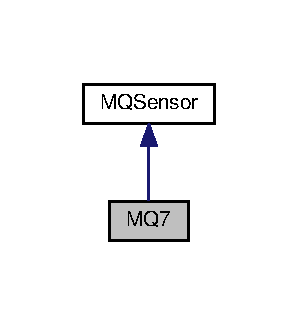
\includegraphics[width=143pt]{class_m_q7__inherit__graph}
\end{center}
\end{figure}


Collaboration diagram for M\+Q7\+:\nopagebreak
\begin{figure}[H]
\begin{center}
\leavevmode
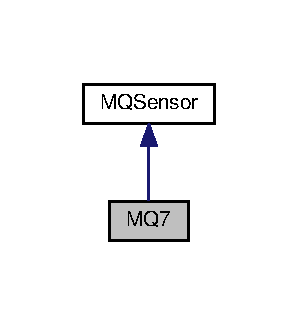
\includegraphics[width=143pt]{class_m_q7__coll__graph}
\end{center}
\end{figure}
\subsection*{Public Member Functions}
\begin{DoxyCompactItemize}
\item 
\hyperlink{class_m_q7_a883b2f95cfa65f7ab734057d0d8e4797}{M\+Q7} (const uint8\+\_\+t mqpin)
\item 
float \hyperlink{class_m_q7_a985699da69427048ea6a01720c79bc2e}{read\+H2} ()
\item 
float \hyperlink{class_m_q7_a3ce5efda2320dfb57667e37767b0d570}{read\+Carbon\+Monoxide} ()
\end{DoxyCompactItemize}
\subsection*{Additional Inherited Members}


\subsection{Detailed Description}
The class of the \hyperlink{class_m_q7}{M\+Q7} sensor, with it\textquotesingle{}s relevant data.

\begin{DoxyAuthor}{Author}
Daniel Pereira Poltronieri 
\end{DoxyAuthor}
\begin{DoxyDate}{Date}
October, 2017 Contact\+: \href{mailto:danppoltronieri@gmail.com}{\tt danppoltronieri@gmail.\+com} 
\end{DoxyDate}


Definition at line 197 of file M\+Q\+Sensor.\+hpp.



\subsection{Constructor \& Destructor Documentation}
\index{M\+Q7@{M\+Q7}!M\+Q7@{M\+Q7}}
\index{M\+Q7@{M\+Q7}!M\+Q7@{M\+Q7}}
\subsubsection[{\texorpdfstring{M\+Q7(const uint8\+\_\+t mqpin)}{MQ7(const uint8_t mqpin)}}]{\setlength{\rightskip}{0pt plus 5cm}M\+Q7\+::\+M\+Q7 (
\begin{DoxyParamCaption}
\item[{const uint8\+\_\+t}]{mqpin}
\end{DoxyParamCaption}
)}\hypertarget{class_m_q7_a883b2f95cfa65f7ab734057d0d8e4797}{}\label{class_m_q7_a883b2f95cfa65f7ab734057d0d8e4797}
\hyperlink{class_m_q7_a883b2f95cfa65f7ab734057d0d8e4797}{M\+Q7\+::\+M\+Q7} constructor. 
\begin{DoxyParams}{Parameters}
{\em mqpin} & The arduino pin to which the sensor is connected. \\
\hline
\end{DoxyParams}


Definition at line 310 of file M\+Q\+Sensor.\+cpp.



\subsection{Member Function Documentation}
\index{M\+Q7@{M\+Q7}!read\+Carbon\+Monoxide@{read\+Carbon\+Monoxide}}
\index{read\+Carbon\+Monoxide@{read\+Carbon\+Monoxide}!M\+Q7@{M\+Q7}}
\subsubsection[{\texorpdfstring{read\+Carbon\+Monoxide()}{readCarbonMonoxide()}}]{\setlength{\rightskip}{0pt plus 5cm}float M\+Q7\+::read\+Carbon\+Monoxide (
\begin{DoxyParamCaption}
{}
\end{DoxyParamCaption}
)}\hypertarget{class_m_q7_a3ce5efda2320dfb57667e37767b0d570}{}\label{class_m_q7_a3ce5efda2320dfb57667e37767b0d570}
Checks if the current data is old, then proceeds to either checking the sensor for the current value or returns the stored value. \begin{DoxyReturn}{Returns}
The most recent Carbon Monoxide data point. 
\end{DoxyReturn}


Definition at line 335 of file M\+Q\+Sensor.\+cpp.

\index{M\+Q7@{M\+Q7}!read\+H2@{read\+H2}}
\index{read\+H2@{read\+H2}!M\+Q7@{M\+Q7}}
\subsubsection[{\texorpdfstring{read\+H2()}{readH2()}}]{\setlength{\rightskip}{0pt plus 5cm}float M\+Q7\+::read\+H2 (
\begin{DoxyParamCaption}
{}
\end{DoxyParamCaption}
)}\hypertarget{class_m_q7_a985699da69427048ea6a01720c79bc2e}{}\label{class_m_q7_a985699da69427048ea6a01720c79bc2e}
Checks if the current data is old, then proceeds to either checking the sensor for the current value or returns the stored value. \begin{DoxyReturn}{Returns}
The most recent H2 data point. 
\end{DoxyReturn}


Definition at line 321 of file M\+Q\+Sensor.\+cpp.



The documentation for this class was generated from the following files\+:\begin{DoxyCompactItemize}
\item 
lib/\+M\+Q-\/\+Sensor/src/\hyperlink{_m_q_sensor_8hpp}{M\+Q\+Sensor.\+hpp}\item 
lib/\+M\+Q-\/\+Sensor/src/\hyperlink{_m_q_sensor_8cpp}{M\+Q\+Sensor.\+cpp}\end{DoxyCompactItemize}

\hypertarget{class_m_q_dummy}{}\section{M\+Q\+Dummy Class Reference}
\label{class_m_q_dummy}\index{M\+Q\+Dummy@{M\+Q\+Dummy}}


{\ttfamily \#include $<$M\+Q\+Sensor.\+hpp$>$}



Inheritance diagram for M\+Q\+Dummy\+:
% FIG 0


Collaboration diagram for M\+Q\+Dummy\+:
% FIG 1
\subsection*{Public Member Functions}
\begin{DoxyCompactItemize}
\item 
\hyperlink{class_m_q_dummy_acd45bbb9678e3578b0600ecaa74f0120}{M\+Q\+Dummy} (const uint8\+\_\+t mqpin)
\item 
uint16\+\_\+t \hyperlink{class_m_q_dummy_a36c209a1aae7acd690da607677a90181}{check} (void)
\end{DoxyCompactItemize}
\subsection*{Protected Attributes}
\begin{DoxyCompactItemize}
\item 
uint16\+\_\+t \hyperlink{class_m_q_dummy_af00eaac2153761e9bbdf201d95bf415a}{\+\_\+current\+\_\+value}
\end{DoxyCompactItemize}
\subsection*{Additional Inherited Members}


\subsection{Detailed Description}


Definition at line 84 of file M\+Q\+Sensor.\+hpp.



\subsection{Constructor \& Destructor Documentation}
\index{M\+Q\+Dummy@{M\+Q\+Dummy}!M\+Q\+Dummy@{M\+Q\+Dummy}}
\index{M\+Q\+Dummy@{M\+Q\+Dummy}!M\+Q\+Dummy@{M\+Q\+Dummy}}
\subsubsection[{\texorpdfstring{M\+Q\+Dummy(const uint8\+\_\+t mqpin)}{MQDummy(const uint8_t mqpin)}}]{\setlength{\rightskip}{0pt plus 5cm}M\+Q\+Dummy\+::\+M\+Q\+Dummy (
\begin{DoxyParamCaption}
\item[{const uint8\+\_\+t}]{mqpin}
\end{DoxyParamCaption}
)}\hypertarget{class_m_q_dummy_acd45bbb9678e3578b0600ecaa74f0120}{}\label{class_m_q_dummy_acd45bbb9678e3578b0600ecaa74f0120}


Definition at line 169 of file M\+Q\+Sensor.\+cpp.



\subsection{Member Function Documentation}
\index{M\+Q\+Dummy@{M\+Q\+Dummy}!check@{check}}
\index{check@{check}!M\+Q\+Dummy@{M\+Q\+Dummy}}
\subsubsection[{\texorpdfstring{check(void)}{check(void)}}]{\setlength{\rightskip}{0pt plus 5cm}uint16\+\_\+t M\+Q\+Dummy\+::check (
\begin{DoxyParamCaption}
\item[{void}]{}
\end{DoxyParamCaption}
)\hspace{0.3cm}{\ttfamily [inline]}}\hypertarget{class_m_q_dummy_a36c209a1aae7acd690da607677a90181}{}\label{class_m_q_dummy_a36c209a1aae7acd690da607677a90181}


Definition at line 90 of file M\+Q\+Sensor.\+hpp.



\subsection{Member Data Documentation}
\index{M\+Q\+Dummy@{M\+Q\+Dummy}!\+\_\+current\+\_\+value@{\+\_\+current\+\_\+value}}
\index{\+\_\+current\+\_\+value@{\+\_\+current\+\_\+value}!M\+Q\+Dummy@{M\+Q\+Dummy}}
\subsubsection[{\texorpdfstring{\+\_\+current\+\_\+value}{_current_value}}]{\setlength{\rightskip}{0pt plus 5cm}uint16\+\_\+t M\+Q\+Dummy\+::\+\_\+current\+\_\+value\hspace{0.3cm}{\ttfamily [protected]}}\hypertarget{class_m_q_dummy_af00eaac2153761e9bbdf201d95bf415a}{}\label{class_m_q_dummy_af00eaac2153761e9bbdf201d95bf415a}


Definition at line 97 of file M\+Q\+Sensor.\+hpp.



The documentation for this class was generated from the following files\+:\begin{DoxyCompactItemize}
\item 
lib/\+M\+Q-\/\+Sensor/src/\hyperlink{_m_q_sensor_8hpp}{M\+Q\+Sensor.\+hpp}\item 
lib/\+M\+Q-\/\+Sensor/src/\hyperlink{_m_q_sensor_8cpp}{M\+Q\+Sensor.\+cpp}\end{DoxyCompactItemize}

\hypertarget{class_m_q_potentiometer}{}\section{M\+Q\+Potentiometer Class Reference}
\label{class_m_q_potentiometer}\index{M\+Q\+Potentiometer@{M\+Q\+Potentiometer}}


{\ttfamily \#include $<$M\+Q\+Sensor.\+hpp$>$}



Inheritance diagram for M\+Q\+Potentiometer\+:\nopagebreak
\begin{figure}[H]
\begin{center}
\leavevmode
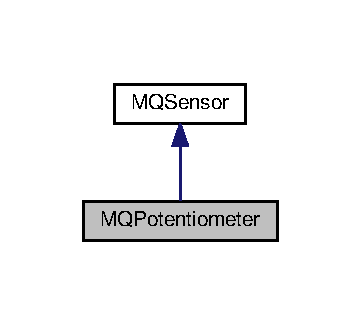
\includegraphics[width=173pt]{class_m_q_potentiometer__inherit__graph}
\end{center}
\end{figure}


Collaboration diagram for M\+Q\+Potentiometer\+:\nopagebreak
\begin{figure}[H]
\begin{center}
\leavevmode
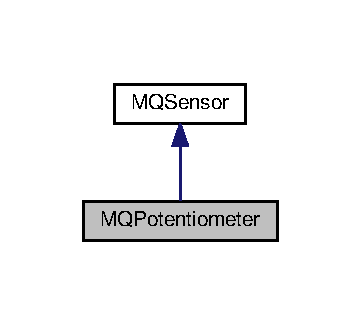
\includegraphics[width=173pt]{class_m_q_potentiometer__coll__graph}
\end{center}
\end{figure}
\subsection*{Public Member Functions}
\begin{DoxyCompactItemize}
\item 
\hyperlink{class_m_q_potentiometer_a9a890ae1eee63b533f2865fcc82a5e66}{M\+Q\+Potentiometer} (const uint8\+\_\+t mqpin)
\end{DoxyCompactItemize}
\subsection*{Additional Inherited Members}


\subsection{Detailed Description}
This uses a potentiometer as a sensor, to be used to generate values for debugging purposes. May be of better use if expandanded to handle a gas curve.

\begin{DoxyAuthor}{Author}
Daniel Pereira Poltronieri 
\end{DoxyAuthor}
\begin{DoxyDate}{Date}
October, 2017 Contact\+: \href{mailto:danppoltronieri@gmail.com}{\tt danppoltronieri@gmail.\+com} 
\end{DoxyDate}


Definition at line 150 of file M\+Q\+Sensor.\+hpp.



\subsection{Constructor \& Destructor Documentation}
\index{M\+Q\+Potentiometer@{M\+Q\+Potentiometer}!M\+Q\+Potentiometer@{M\+Q\+Potentiometer}}
\index{M\+Q\+Potentiometer@{M\+Q\+Potentiometer}!M\+Q\+Potentiometer@{M\+Q\+Potentiometer}}
\subsubsection[{\texorpdfstring{M\+Q\+Potentiometer(const uint8\+\_\+t mqpin)}{MQPotentiometer(const uint8_t mqpin)}}]{\setlength{\rightskip}{0pt plus 5cm}M\+Q\+Potentiometer\+::\+M\+Q\+Potentiometer (
\begin{DoxyParamCaption}
\item[{const uint8\+\_\+t}]{mqpin}
\end{DoxyParamCaption}
)}\hypertarget{class_m_q_potentiometer_a9a890ae1eee63b533f2865fcc82a5e66}{}\label{class_m_q_potentiometer_a9a890ae1eee63b533f2865fcc82a5e66}


Definition at line 270 of file M\+Q\+Sensor.\+cpp.



The documentation for this class was generated from the following files\+:\begin{DoxyCompactItemize}
\item 
lib/\+M\+Q-\/\+Sensor/src/\hyperlink{_m_q_sensor_8hpp}{M\+Q\+Sensor.\+hpp}\item 
lib/\+M\+Q-\/\+Sensor/src/\hyperlink{_m_q_sensor_8cpp}{M\+Q\+Sensor.\+cpp}\end{DoxyCompactItemize}

\hypertarget{class_m_q_sensor}{}\section{M\+Q\+Sensor Class Reference}
\label{class_m_q_sensor}\index{M\+Q\+Sensor@{M\+Q\+Sensor}}


{\ttfamily \#include $<$M\+Q\+Sensor.\+hpp$>$}



Inheritance diagram for M\+Q\+Sensor\+:
% FIG 0
\subsection*{Public Member Functions}
\begin{DoxyCompactItemize}
\item 
uint16\+\_\+t \hyperlink{class_m_q_sensor_acc2b495b544c2e801a4708c91df7a874}{check} (void)
\item 
void \hyperlink{class_m_q_sensor_ae6d1b0181e6769745caf5766ceef1522}{begin} ()
\item 
void \hyperlink{class_m_q_sensor_a54d01cd9465f177f431f070f7e96821d}{set\+Rl\+Value} (const uint8\+\_\+t rlvalue)
\item 
void \hyperlink{class_m_q_sensor_ad93e118f8bce230241af72307a7c2b79}{set\+Calibration\+Sample\+Times} (const uint8\+\_\+t cst)
\item 
void \hyperlink{class_m_q_sensor_ad14ad2558241aac29113e13b8a5137f7}{set\+Calibration\+Sample\+Interval} (const uint8\+\_\+t csi)
\item 
void \hyperlink{class_m_q_sensor_acefcf4fca770e50814f32bac2c80459c}{set\+Read\+Sample\+Interval} (const uint8\+\_\+t rsi)
\item 
void \hyperlink{class_m_q_sensor_a8e4a65e66a55f8abbe4365400e27ab97}{set\+Read\+Sample\+Times} (const uint8\+\_\+t rst)
\item 
void \hyperlink{class_m_q_sensor_a03eb97a82d462ee54ed249bc11da916a}{Set\+Ro} (const float ro\+\_\+factor)
\item 
void \hyperlink{class_m_q_sensor_a870f6dacc4896cdea8cb114b3b508ea3}{Set\+Ro\+Clean\+Air\+Factor} (const float ro\+\_\+clean\+\_\+air\+\_\+factor)
\item 
float const \hyperlink{class_m_q_sensor_a48389f7f5b5757092f7ae7a0893fe33f}{Get\+Ro\+Clean\+Air\+Factor} (void)
\item 
float const \hyperlink{class_m_q_sensor_a7292dbbdb30f7dac813f16009b6cd282}{Get\+Ro} (void)
\end{DoxyCompactItemize}
\subsection*{Static Public Member Functions}
\begin{DoxyCompactItemize}
\item 
static \hyperlink{class_m_q_sensor}{M\+Q\+Sensor} \hyperlink{class_m_q_sensor_a7f29aed48ad89d8403f08a4e83b136b5}{New\+M\+Q\+Sensor} (const uint8\+\_\+t mqpin, const uint8\+\_\+t mqtype)
\end{DoxyCompactItemize}
\subsection*{Protected Member Functions}
\begin{DoxyCompactItemize}
\item 
\hyperlink{class_m_q_sensor_a58bc8dbc8dc2e97584a34f1a545f93e1}{M\+Q\+Sensor} (const uint8\+\_\+t mqpin)
\item 
float const \hyperlink{class_m_q_sensor_ac769cc3eade7067313d185848f63f2cf}{M\+Q\+Read} ()
\item 
float const \hyperlink{class_m_q_sensor_a92ef594a160b257ca124481a21840a96}{M\+Q\+Get\+Percentage} (const float rs\+\_\+ro\+\_\+ratio, const float $\ast$pcurve)
\item 
float \hyperlink{class_m_q_sensor_aae67f9f2749712bd2afa90a2a97a29fd}{M\+Q\+Calibration} ()
\item 
float const \hyperlink{class_m_q_sensor_a1bb39a92869446ede5ba1c6854034e20}{M\+Q\+Resistance\+Calculation} (const int raw\+\_\+adc)
\end{DoxyCompactItemize}
\subsection*{Protected Attributes}
\begin{DoxyCompactItemize}
\item 
size\+\_\+t \hyperlink{class_m_q_sensor_a464b0db94d80b771efca70a0eb58f951}{\+\_\+\+L\+A\+S\+T\+\_\+\+R\+E\+A\+D\+\_\+\+T\+I\+ME} = 0
\item 
size\+\_\+t \hyperlink{class_m_q_sensor_a4a8e710f1bc61afb702d26ceb1366f11}{\+\_\+\+R\+E\+A\+D\+\_\+\+S\+E\+N\+S\+O\+R\+\_\+\+I\+N\+T\+E\+R\+V\+AL} = 10000
\item 
uint8\+\_\+t \hyperlink{class_m_q_sensor_aaa75c5a8dbb6b8bfba63a7b8749acd82}{\+\_\+\+M\+Q\+\_\+pin}
\item 
uint8\+\_\+t \hyperlink{class_m_q_sensor_ae04756d16f8d90e492fdb48c5ac4e930}{\+\_\+\+C\+A\+L\+I\+B\+A\+R\+A\+I\+O\+N\+\_\+\+S\+A\+M\+P\+L\+E\+\_\+\+T\+I\+M\+ES} = 5
\item 
uint8\+\_\+t \hyperlink{class_m_q_sensor_a440f40e2d8109c9cda26ce2b3d8ff564}{\+\_\+\+C\+A\+L\+I\+B\+R\+A\+T\+I\+O\+N\+\_\+\+S\+A\+M\+P\+L\+E\+\_\+\+I\+N\+T\+E\+R\+V\+AL} = 50
\item 
uint8\+\_\+t \hyperlink{class_m_q_sensor_a7dcb6e9f9ff88b498d7b47dd33b0809f}{\+\_\+\+R\+E\+A\+D\+\_\+\+S\+A\+M\+P\+L\+E\+\_\+\+I\+N\+T\+E\+R\+V\+AL} = 50
\item 
uint8\+\_\+t \hyperlink{class_m_q_sensor_a3c6ba8a07087b67ee99941bced73e940}{\+\_\+\+R\+E\+A\+D\+\_\+\+S\+A\+M\+P\+L\+E\+\_\+\+T\+I\+M\+ES} = 5
\item 
float \hyperlink{class_m_q_sensor_adc7e7af2139868a784d31d27d73b7df3}{\+\_\+\+R\+O\+\_\+\+C\+L\+E\+A\+N\+\_\+\+A\+I\+R\+\_\+\+F\+A\+C\+T\+OR} = 9.\+83
\item 
float \hyperlink{class_m_q_sensor_ade2e483ebc557d1caf753d41a8b3afde}{\+\_\+\+Ro} = 10
\item 
float \hyperlink{class_m_q_sensor_a2cf9585b95f5beaac2dc8edbab7eff42}{\+\_\+\+R\+L\+\_\+\+V\+A\+L\+UE} = 5
\end{DoxyCompactItemize}


\subsection{Detailed Description}


Definition at line 35 of file M\+Q\+Sensor.\+hpp.



\subsection{Constructor \& Destructor Documentation}
\index{M\+Q\+Sensor@{M\+Q\+Sensor}!M\+Q\+Sensor@{M\+Q\+Sensor}}
\index{M\+Q\+Sensor@{M\+Q\+Sensor}!M\+Q\+Sensor@{M\+Q\+Sensor}}
\subsubsection[{\texorpdfstring{M\+Q\+Sensor(const uint8\+\_\+t mqpin)}{MQSensor(const uint8_t mqpin)}}]{\setlength{\rightskip}{0pt plus 5cm}M\+Q\+Sensor\+::\+M\+Q\+Sensor (
\begin{DoxyParamCaption}
\item[{const uint8\+\_\+t}]{mqpin}
\end{DoxyParamCaption}
)\hspace{0.3cm}{\ttfamily [protected]}}\hypertarget{class_m_q_sensor_a58bc8dbc8dc2e97584a34f1a545f93e1}{}\label{class_m_q_sensor_a58bc8dbc8dc2e97584a34f1a545f93e1}


Definition at line 29 of file M\+Q\+Sensor.\+cpp.



\subsection{Member Function Documentation}
\index{M\+Q\+Sensor@{M\+Q\+Sensor}!begin@{begin}}
\index{begin@{begin}!M\+Q\+Sensor@{M\+Q\+Sensor}}
\subsubsection[{\texorpdfstring{begin()}{begin()}}]{\setlength{\rightskip}{0pt plus 5cm}void M\+Q\+Sensor\+::begin (
\begin{DoxyParamCaption}
{}
\end{DoxyParamCaption}
)}\hypertarget{class_m_q_sensor_ae6d1b0181e6769745caf5766ceef1522}{}\label{class_m_q_sensor_ae6d1b0181e6769745caf5766ceef1522}


Definition at line 75 of file M\+Q\+Sensor.\+cpp.



Here is the call graph for this function\+:
% FIG 1




Here is the caller graph for this function\+:
% FIG 2


\index{M\+Q\+Sensor@{M\+Q\+Sensor}!check@{check}}
\index{check@{check}!M\+Q\+Sensor@{M\+Q\+Sensor}}
\subsubsection[{\texorpdfstring{check(void)}{check(void)}}]{\setlength{\rightskip}{0pt plus 5cm}uint16\+\_\+t M\+Q\+Sensor\+::check (
\begin{DoxyParamCaption}
\item[{void}]{}
\end{DoxyParamCaption}
)\hspace{0.3cm}{\ttfamily [inline]}}\hypertarget{class_m_q_sensor_acc2b495b544c2e801a4708c91df7a874}{}\label{class_m_q_sensor_acc2b495b544c2e801a4708c91df7a874}


Definition at line 43 of file M\+Q\+Sensor.\+hpp.



Here is the call graph for this function\+:
% FIG 3




Here is the caller graph for this function\+:
% FIG 4


\index{M\+Q\+Sensor@{M\+Q\+Sensor}!Get\+Ro@{Get\+Ro}}
\index{Get\+Ro@{Get\+Ro}!M\+Q\+Sensor@{M\+Q\+Sensor}}
\subsubsection[{\texorpdfstring{Get\+Ro(void)}{GetRo(void)}}]{\setlength{\rightskip}{0pt plus 5cm}float const M\+Q\+Sensor\+::\+Get\+Ro (
\begin{DoxyParamCaption}
\item[{void}]{}
\end{DoxyParamCaption}
)}\hypertarget{class_m_q_sensor_a7292dbbdb30f7dac813f16009b6cd282}{}\label{class_m_q_sensor_a7292dbbdb30f7dac813f16009b6cd282}


Definition at line 70 of file M\+Q\+Sensor.\+cpp.



Here is the caller graph for this function\+:
% FIG 5


\index{M\+Q\+Sensor@{M\+Q\+Sensor}!Get\+Ro\+Clean\+Air\+Factor@{Get\+Ro\+Clean\+Air\+Factor}}
\index{Get\+Ro\+Clean\+Air\+Factor@{Get\+Ro\+Clean\+Air\+Factor}!M\+Q\+Sensor@{M\+Q\+Sensor}}
\subsubsection[{\texorpdfstring{Get\+Ro\+Clean\+Air\+Factor(void)}{GetRoCleanAirFactor(void)}}]{\setlength{\rightskip}{0pt plus 5cm}float const M\+Q\+Sensor\+::\+Get\+Ro\+Clean\+Air\+Factor (
\begin{DoxyParamCaption}
\item[{void}]{}
\end{DoxyParamCaption}
)}\hypertarget{class_m_q_sensor_a48389f7f5b5757092f7ae7a0893fe33f}{}\label{class_m_q_sensor_a48389f7f5b5757092f7ae7a0893fe33f}


Definition at line 67 of file M\+Q\+Sensor.\+cpp.



Here is the caller graph for this function\+:
% FIG 6


\index{M\+Q\+Sensor@{M\+Q\+Sensor}!M\+Q\+Calibration@{M\+Q\+Calibration}}
\index{M\+Q\+Calibration@{M\+Q\+Calibration}!M\+Q\+Sensor@{M\+Q\+Sensor}}
\subsubsection[{\texorpdfstring{M\+Q\+Calibration()}{MQCalibration()}}]{\setlength{\rightskip}{0pt plus 5cm}float M\+Q\+Sensor\+::\+M\+Q\+Calibration (
\begin{DoxyParamCaption}
{}
\end{DoxyParamCaption}
)\hspace{0.3cm}{\ttfamily [protected]}}\hypertarget{class_m_q_sensor_aae67f9f2749712bd2afa90a2a97a29fd}{}\label{class_m_q_sensor_aae67f9f2749712bd2afa90a2a97a29fd}


Definition at line 123 of file M\+Q\+Sensor.\+cpp.



Here is the call graph for this function\+:
% FIG 7




Here is the caller graph for this function\+:
% FIG 8


\index{M\+Q\+Sensor@{M\+Q\+Sensor}!M\+Q\+Get\+Percentage@{M\+Q\+Get\+Percentage}}
\index{M\+Q\+Get\+Percentage@{M\+Q\+Get\+Percentage}!M\+Q\+Sensor@{M\+Q\+Sensor}}
\subsubsection[{\texorpdfstring{M\+Q\+Get\+Percentage(const float rs\+\_\+ro\+\_\+ratio, const float $\ast$pcurve)}{MQGetPercentage(const float rs_ro_ratio, const float *pcurve)}}]{\setlength{\rightskip}{0pt plus 5cm}float const M\+Q\+Sensor\+::\+M\+Q\+Get\+Percentage (
\begin{DoxyParamCaption}
\item[{const float}]{rs\+\_\+ro\+\_\+ratio, }
\item[{const float $\ast$}]{pcurve}
\end{DoxyParamCaption}
)\hspace{0.3cm}{\ttfamily [protected]}}\hypertarget{class_m_q_sensor_a92ef594a160b257ca124481a21840a96}{}\label{class_m_q_sensor_a92ef594a160b257ca124481a21840a96}


Definition at line 161 of file M\+Q\+Sensor.\+cpp.



Here is the caller graph for this function\+:
% FIG 9


\index{M\+Q\+Sensor@{M\+Q\+Sensor}!M\+Q\+Read@{M\+Q\+Read}}
\index{M\+Q\+Read@{M\+Q\+Read}!M\+Q\+Sensor@{M\+Q\+Sensor}}
\subsubsection[{\texorpdfstring{M\+Q\+Read()}{MQRead()}}]{\setlength{\rightskip}{0pt plus 5cm}float const M\+Q\+Sensor\+::\+M\+Q\+Read (
\begin{DoxyParamCaption}
{}
\end{DoxyParamCaption}
)\hspace{0.3cm}{\ttfamily [protected]}}\hypertarget{class_m_q_sensor_ac769cc3eade7067313d185848f63f2cf}{}\label{class_m_q_sensor_ac769cc3eade7067313d185848f63f2cf}


Definition at line 138 of file M\+Q\+Sensor.\+cpp.



Here is the call graph for this function\+:
% FIG 10




Here is the caller graph for this function\+:
% FIG 11


\index{M\+Q\+Sensor@{M\+Q\+Sensor}!M\+Q\+Resistance\+Calculation@{M\+Q\+Resistance\+Calculation}}
\index{M\+Q\+Resistance\+Calculation@{M\+Q\+Resistance\+Calculation}!M\+Q\+Sensor@{M\+Q\+Sensor}}
\subsubsection[{\texorpdfstring{M\+Q\+Resistance\+Calculation(const int raw\+\_\+adc)}{MQResistanceCalculation(const int raw_adc)}}]{\setlength{\rightskip}{0pt plus 5cm}float const M\+Q\+Sensor\+::\+M\+Q\+Resistance\+Calculation (
\begin{DoxyParamCaption}
\item[{const int}]{raw\+\_\+adc}
\end{DoxyParamCaption}
)\hspace{0.3cm}{\ttfamily [inline]}, {\ttfamily [protected]}}\hypertarget{class_m_q_sensor_a1bb39a92869446ede5ba1c6854034e20}{}\label{class_m_q_sensor_a1bb39a92869446ede5ba1c6854034e20}


Definition at line 92 of file M\+Q\+Sensor.\+cpp.



Here is the caller graph for this function\+:
% FIG 12


\index{M\+Q\+Sensor@{M\+Q\+Sensor}!New\+M\+Q\+Sensor@{New\+M\+Q\+Sensor}}
\index{New\+M\+Q\+Sensor@{New\+M\+Q\+Sensor}!M\+Q\+Sensor@{M\+Q\+Sensor}}
\subsubsection[{\texorpdfstring{New\+M\+Q\+Sensor(const uint8\+\_\+t mqpin, const uint8\+\_\+t mqtype)}{NewMQSensor(const uint8_t mqpin, const uint8_t mqtype)}}]{\setlength{\rightskip}{0pt plus 5cm}{\bf M\+Q\+Sensor} M\+Q\+Sensor\+::\+New\+M\+Q\+Sensor (
\begin{DoxyParamCaption}
\item[{const uint8\+\_\+t}]{mqpin, }
\item[{const uint8\+\_\+t}]{mqtype}
\end{DoxyParamCaption}
)\hspace{0.3cm}{\ttfamily [static]}}\hypertarget{class_m_q_sensor_a7f29aed48ad89d8403f08a4e83b136b5}{}\label{class_m_q_sensor_a7f29aed48ad89d8403f08a4e83b136b5}


Definition at line 7 of file M\+Q\+Sensor.\+cpp.

\index{M\+Q\+Sensor@{M\+Q\+Sensor}!set\+Calibration\+Sample\+Interval@{set\+Calibration\+Sample\+Interval}}
\index{set\+Calibration\+Sample\+Interval@{set\+Calibration\+Sample\+Interval}!M\+Q\+Sensor@{M\+Q\+Sensor}}
\subsubsection[{\texorpdfstring{set\+Calibration\+Sample\+Interval(const uint8\+\_\+t csi)}{setCalibrationSampleInterval(const uint8_t csi)}}]{\setlength{\rightskip}{0pt plus 5cm}void M\+Q\+Sensor\+::set\+Calibration\+Sample\+Interval (
\begin{DoxyParamCaption}
\item[{const uint8\+\_\+t}]{csi}
\end{DoxyParamCaption}
)}\hypertarget{class_m_q_sensor_ad14ad2558241aac29113e13b8a5137f7}{}\label{class_m_q_sensor_ad14ad2558241aac29113e13b8a5137f7}


Definition at line 58 of file M\+Q\+Sensor.\+cpp.



Here is the caller graph for this function\+:
% FIG 13


\index{M\+Q\+Sensor@{M\+Q\+Sensor}!set\+Calibration\+Sample\+Times@{set\+Calibration\+Sample\+Times}}
\index{set\+Calibration\+Sample\+Times@{set\+Calibration\+Sample\+Times}!M\+Q\+Sensor@{M\+Q\+Sensor}}
\subsubsection[{\texorpdfstring{set\+Calibration\+Sample\+Times(const uint8\+\_\+t cst)}{setCalibrationSampleTimes(const uint8_t cst)}}]{\setlength{\rightskip}{0pt plus 5cm}void M\+Q\+Sensor\+::set\+Calibration\+Sample\+Times (
\begin{DoxyParamCaption}
\item[{const uint8\+\_\+t}]{cst}
\end{DoxyParamCaption}
)}\hypertarget{class_m_q_sensor_ad93e118f8bce230241af72307a7c2b79}{}\label{class_m_q_sensor_ad93e118f8bce230241af72307a7c2b79}


Definition at line 55 of file M\+Q\+Sensor.\+cpp.



Here is the caller graph for this function\+:
% FIG 14


\index{M\+Q\+Sensor@{M\+Q\+Sensor}!set\+Read\+Sample\+Interval@{set\+Read\+Sample\+Interval}}
\index{set\+Read\+Sample\+Interval@{set\+Read\+Sample\+Interval}!M\+Q\+Sensor@{M\+Q\+Sensor}}
\subsubsection[{\texorpdfstring{set\+Read\+Sample\+Interval(const uint8\+\_\+t rsi)}{setReadSampleInterval(const uint8_t rsi)}}]{\setlength{\rightskip}{0pt plus 5cm}void M\+Q\+Sensor\+::set\+Read\+Sample\+Interval (
\begin{DoxyParamCaption}
\item[{const uint8\+\_\+t}]{rsi}
\end{DoxyParamCaption}
)}\hypertarget{class_m_q_sensor_acefcf4fca770e50814f32bac2c80459c}{}\label{class_m_q_sensor_acefcf4fca770e50814f32bac2c80459c}


Definition at line 61 of file M\+Q\+Sensor.\+cpp.



Here is the caller graph for this function\+:
% FIG 15


\index{M\+Q\+Sensor@{M\+Q\+Sensor}!set\+Read\+Sample\+Times@{set\+Read\+Sample\+Times}}
\index{set\+Read\+Sample\+Times@{set\+Read\+Sample\+Times}!M\+Q\+Sensor@{M\+Q\+Sensor}}
\subsubsection[{\texorpdfstring{set\+Read\+Sample\+Times(const uint8\+\_\+t rst)}{setReadSampleTimes(const uint8_t rst)}}]{\setlength{\rightskip}{0pt plus 5cm}void M\+Q\+Sensor\+::set\+Read\+Sample\+Times (
\begin{DoxyParamCaption}
\item[{const uint8\+\_\+t}]{rst}
\end{DoxyParamCaption}
)}\hypertarget{class_m_q_sensor_a8e4a65e66a55f8abbe4365400e27ab97}{}\label{class_m_q_sensor_a8e4a65e66a55f8abbe4365400e27ab97}


Definition at line 64 of file M\+Q\+Sensor.\+cpp.



Here is the caller graph for this function\+:
% FIG 16


\index{M\+Q\+Sensor@{M\+Q\+Sensor}!set\+Rl\+Value@{set\+Rl\+Value}}
\index{set\+Rl\+Value@{set\+Rl\+Value}!M\+Q\+Sensor@{M\+Q\+Sensor}}
\subsubsection[{\texorpdfstring{set\+Rl\+Value(const uint8\+\_\+t rlvalue)}{setRlValue(const uint8_t rlvalue)}}]{\setlength{\rightskip}{0pt plus 5cm}void M\+Q\+Sensor\+::set\+Rl\+Value (
\begin{DoxyParamCaption}
\item[{const uint8\+\_\+t}]{rlvalue}
\end{DoxyParamCaption}
)}\hypertarget{class_m_q_sensor_a54d01cd9465f177f431f070f7e96821d}{}\label{class_m_q_sensor_a54d01cd9465f177f431f070f7e96821d}


Definition at line 52 of file M\+Q\+Sensor.\+cpp.



Here is the caller graph for this function\+:
% FIG 17


\index{M\+Q\+Sensor@{M\+Q\+Sensor}!Set\+Ro@{Set\+Ro}}
\index{Set\+Ro@{Set\+Ro}!M\+Q\+Sensor@{M\+Q\+Sensor}}
\subsubsection[{\texorpdfstring{Set\+Ro(const float ro\+\_\+factor)}{SetRo(const float ro_factor)}}]{\setlength{\rightskip}{0pt plus 5cm}void M\+Q\+Sensor\+::\+Set\+Ro (
\begin{DoxyParamCaption}
\item[{const float}]{ro\+\_\+factor}
\end{DoxyParamCaption}
)}\hypertarget{class_m_q_sensor_a03eb97a82d462ee54ed249bc11da916a}{}\label{class_m_q_sensor_a03eb97a82d462ee54ed249bc11da916a}


Definition at line 46 of file M\+Q\+Sensor.\+cpp.



Here is the caller graph for this function\+:
% FIG 18


\index{M\+Q\+Sensor@{M\+Q\+Sensor}!Set\+Ro\+Clean\+Air\+Factor@{Set\+Ro\+Clean\+Air\+Factor}}
\index{Set\+Ro\+Clean\+Air\+Factor@{Set\+Ro\+Clean\+Air\+Factor}!M\+Q\+Sensor@{M\+Q\+Sensor}}
\subsubsection[{\texorpdfstring{Set\+Ro\+Clean\+Air\+Factor(const float ro\+\_\+clean\+\_\+air\+\_\+factor)}{SetRoCleanAirFactor(const float ro_clean_air_factor)}}]{\setlength{\rightskip}{0pt plus 5cm}void M\+Q\+Sensor\+::\+Set\+Ro\+Clean\+Air\+Factor (
\begin{DoxyParamCaption}
\item[{const float}]{ro\+\_\+clean\+\_\+air\+\_\+factor}
\end{DoxyParamCaption}
)}\hypertarget{class_m_q_sensor_a870f6dacc4896cdea8cb114b3b508ea3}{}\label{class_m_q_sensor_a870f6dacc4896cdea8cb114b3b508ea3}


Definition at line 49 of file M\+Q\+Sensor.\+cpp.



Here is the caller graph for this function\+:
% FIG 19




\subsection{Member Data Documentation}
\index{M\+Q\+Sensor@{M\+Q\+Sensor}!\+\_\+\+C\+A\+L\+I\+B\+A\+R\+A\+I\+O\+N\+\_\+\+S\+A\+M\+P\+L\+E\+\_\+\+T\+I\+M\+ES@{\+\_\+\+C\+A\+L\+I\+B\+A\+R\+A\+I\+O\+N\+\_\+\+S\+A\+M\+P\+L\+E\+\_\+\+T\+I\+M\+ES}}
\index{\+\_\+\+C\+A\+L\+I\+B\+A\+R\+A\+I\+O\+N\+\_\+\+S\+A\+M\+P\+L\+E\+\_\+\+T\+I\+M\+ES@{\+\_\+\+C\+A\+L\+I\+B\+A\+R\+A\+I\+O\+N\+\_\+\+S\+A\+M\+P\+L\+E\+\_\+\+T\+I\+M\+ES}!M\+Q\+Sensor@{M\+Q\+Sensor}}
\subsubsection[{\texorpdfstring{\+\_\+\+C\+A\+L\+I\+B\+A\+R\+A\+I\+O\+N\+\_\+\+S\+A\+M\+P\+L\+E\+\_\+\+T\+I\+M\+ES}{_CALIBARAION_SAMPLE_TIMES}}]{\setlength{\rightskip}{0pt plus 5cm}uint8\+\_\+t M\+Q\+Sensor\+::\+\_\+\+C\+A\+L\+I\+B\+A\+R\+A\+I\+O\+N\+\_\+\+S\+A\+M\+P\+L\+E\+\_\+\+T\+I\+M\+ES = 5\hspace{0.3cm}{\ttfamily [protected]}}\hypertarget{class_m_q_sensor_ae04756d16f8d90e492fdb48c5ac4e930}{}\label{class_m_q_sensor_ae04756d16f8d90e492fdb48c5ac4e930}


Definition at line 67 of file M\+Q\+Sensor.\+hpp.

\index{M\+Q\+Sensor@{M\+Q\+Sensor}!\+\_\+\+C\+A\+L\+I\+B\+R\+A\+T\+I\+O\+N\+\_\+\+S\+A\+M\+P\+L\+E\+\_\+\+I\+N\+T\+E\+R\+V\+AL@{\+\_\+\+C\+A\+L\+I\+B\+R\+A\+T\+I\+O\+N\+\_\+\+S\+A\+M\+P\+L\+E\+\_\+\+I\+N\+T\+E\+R\+V\+AL}}
\index{\+\_\+\+C\+A\+L\+I\+B\+R\+A\+T\+I\+O\+N\+\_\+\+S\+A\+M\+P\+L\+E\+\_\+\+I\+N\+T\+E\+R\+V\+AL@{\+\_\+\+C\+A\+L\+I\+B\+R\+A\+T\+I\+O\+N\+\_\+\+S\+A\+M\+P\+L\+E\+\_\+\+I\+N\+T\+E\+R\+V\+AL}!M\+Q\+Sensor@{M\+Q\+Sensor}}
\subsubsection[{\texorpdfstring{\+\_\+\+C\+A\+L\+I\+B\+R\+A\+T\+I\+O\+N\+\_\+\+S\+A\+M\+P\+L\+E\+\_\+\+I\+N\+T\+E\+R\+V\+AL}{_CALIBRATION_SAMPLE_INTERVAL}}]{\setlength{\rightskip}{0pt plus 5cm}uint8\+\_\+t M\+Q\+Sensor\+::\+\_\+\+C\+A\+L\+I\+B\+R\+A\+T\+I\+O\+N\+\_\+\+S\+A\+M\+P\+L\+E\+\_\+\+I\+N\+T\+E\+R\+V\+AL = 50\hspace{0.3cm}{\ttfamily [protected]}}\hypertarget{class_m_q_sensor_a440f40e2d8109c9cda26ce2b3d8ff564}{}\label{class_m_q_sensor_a440f40e2d8109c9cda26ce2b3d8ff564}


Definition at line 68 of file M\+Q\+Sensor.\+hpp.

\index{M\+Q\+Sensor@{M\+Q\+Sensor}!\+\_\+\+L\+A\+S\+T\+\_\+\+R\+E\+A\+D\+\_\+\+T\+I\+ME@{\+\_\+\+L\+A\+S\+T\+\_\+\+R\+E\+A\+D\+\_\+\+T\+I\+ME}}
\index{\+\_\+\+L\+A\+S\+T\+\_\+\+R\+E\+A\+D\+\_\+\+T\+I\+ME@{\+\_\+\+L\+A\+S\+T\+\_\+\+R\+E\+A\+D\+\_\+\+T\+I\+ME}!M\+Q\+Sensor@{M\+Q\+Sensor}}
\subsubsection[{\texorpdfstring{\+\_\+\+L\+A\+S\+T\+\_\+\+R\+E\+A\+D\+\_\+\+T\+I\+ME}{_LAST_READ_TIME}}]{\setlength{\rightskip}{0pt plus 5cm}size\+\_\+t M\+Q\+Sensor\+::\+\_\+\+L\+A\+S\+T\+\_\+\+R\+E\+A\+D\+\_\+\+T\+I\+ME = 0\hspace{0.3cm}{\ttfamily [protected]}}\hypertarget{class_m_q_sensor_a464b0db94d80b771efca70a0eb58f951}{}\label{class_m_q_sensor_a464b0db94d80b771efca70a0eb58f951}


Definition at line 64 of file M\+Q\+Sensor.\+hpp.

\index{M\+Q\+Sensor@{M\+Q\+Sensor}!\+\_\+\+M\+Q\+\_\+pin@{\+\_\+\+M\+Q\+\_\+pin}}
\index{\+\_\+\+M\+Q\+\_\+pin@{\+\_\+\+M\+Q\+\_\+pin}!M\+Q\+Sensor@{M\+Q\+Sensor}}
\subsubsection[{\texorpdfstring{\+\_\+\+M\+Q\+\_\+pin}{_MQ_pin}}]{\setlength{\rightskip}{0pt plus 5cm}uint8\+\_\+t M\+Q\+Sensor\+::\+\_\+\+M\+Q\+\_\+pin\hspace{0.3cm}{\ttfamily [protected]}}\hypertarget{class_m_q_sensor_aaa75c5a8dbb6b8bfba63a7b8749acd82}{}\label{class_m_q_sensor_aaa75c5a8dbb6b8bfba63a7b8749acd82}


Definition at line 66 of file M\+Q\+Sensor.\+hpp.

\index{M\+Q\+Sensor@{M\+Q\+Sensor}!\+\_\+\+R\+E\+A\+D\+\_\+\+S\+A\+M\+P\+L\+E\+\_\+\+I\+N\+T\+E\+R\+V\+AL@{\+\_\+\+R\+E\+A\+D\+\_\+\+S\+A\+M\+P\+L\+E\+\_\+\+I\+N\+T\+E\+R\+V\+AL}}
\index{\+\_\+\+R\+E\+A\+D\+\_\+\+S\+A\+M\+P\+L\+E\+\_\+\+I\+N\+T\+E\+R\+V\+AL@{\+\_\+\+R\+E\+A\+D\+\_\+\+S\+A\+M\+P\+L\+E\+\_\+\+I\+N\+T\+E\+R\+V\+AL}!M\+Q\+Sensor@{M\+Q\+Sensor}}
\subsubsection[{\texorpdfstring{\+\_\+\+R\+E\+A\+D\+\_\+\+S\+A\+M\+P\+L\+E\+\_\+\+I\+N\+T\+E\+R\+V\+AL}{_READ_SAMPLE_INTERVAL}}]{\setlength{\rightskip}{0pt plus 5cm}uint8\+\_\+t M\+Q\+Sensor\+::\+\_\+\+R\+E\+A\+D\+\_\+\+S\+A\+M\+P\+L\+E\+\_\+\+I\+N\+T\+E\+R\+V\+AL = 50\hspace{0.3cm}{\ttfamily [protected]}}\hypertarget{class_m_q_sensor_a7dcb6e9f9ff88b498d7b47dd33b0809f}{}\label{class_m_q_sensor_a7dcb6e9f9ff88b498d7b47dd33b0809f}


Definition at line 69 of file M\+Q\+Sensor.\+hpp.

\index{M\+Q\+Sensor@{M\+Q\+Sensor}!\+\_\+\+R\+E\+A\+D\+\_\+\+S\+A\+M\+P\+L\+E\+\_\+\+T\+I\+M\+ES@{\+\_\+\+R\+E\+A\+D\+\_\+\+S\+A\+M\+P\+L\+E\+\_\+\+T\+I\+M\+ES}}
\index{\+\_\+\+R\+E\+A\+D\+\_\+\+S\+A\+M\+P\+L\+E\+\_\+\+T\+I\+M\+ES@{\+\_\+\+R\+E\+A\+D\+\_\+\+S\+A\+M\+P\+L\+E\+\_\+\+T\+I\+M\+ES}!M\+Q\+Sensor@{M\+Q\+Sensor}}
\subsubsection[{\texorpdfstring{\+\_\+\+R\+E\+A\+D\+\_\+\+S\+A\+M\+P\+L\+E\+\_\+\+T\+I\+M\+ES}{_READ_SAMPLE_TIMES}}]{\setlength{\rightskip}{0pt plus 5cm}uint8\+\_\+t M\+Q\+Sensor\+::\+\_\+\+R\+E\+A\+D\+\_\+\+S\+A\+M\+P\+L\+E\+\_\+\+T\+I\+M\+ES = 5\hspace{0.3cm}{\ttfamily [protected]}}\hypertarget{class_m_q_sensor_a3c6ba8a07087b67ee99941bced73e940}{}\label{class_m_q_sensor_a3c6ba8a07087b67ee99941bced73e940}


Definition at line 70 of file M\+Q\+Sensor.\+hpp.

\index{M\+Q\+Sensor@{M\+Q\+Sensor}!\+\_\+\+R\+E\+A\+D\+\_\+\+S\+E\+N\+S\+O\+R\+\_\+\+I\+N\+T\+E\+R\+V\+AL@{\+\_\+\+R\+E\+A\+D\+\_\+\+S\+E\+N\+S\+O\+R\+\_\+\+I\+N\+T\+E\+R\+V\+AL}}
\index{\+\_\+\+R\+E\+A\+D\+\_\+\+S\+E\+N\+S\+O\+R\+\_\+\+I\+N\+T\+E\+R\+V\+AL@{\+\_\+\+R\+E\+A\+D\+\_\+\+S\+E\+N\+S\+O\+R\+\_\+\+I\+N\+T\+E\+R\+V\+AL}!M\+Q\+Sensor@{M\+Q\+Sensor}}
\subsubsection[{\texorpdfstring{\+\_\+\+R\+E\+A\+D\+\_\+\+S\+E\+N\+S\+O\+R\+\_\+\+I\+N\+T\+E\+R\+V\+AL}{_READ_SENSOR_INTERVAL}}]{\setlength{\rightskip}{0pt plus 5cm}size\+\_\+t M\+Q\+Sensor\+::\+\_\+\+R\+E\+A\+D\+\_\+\+S\+E\+N\+S\+O\+R\+\_\+\+I\+N\+T\+E\+R\+V\+AL = 10000\hspace{0.3cm}{\ttfamily [protected]}}\hypertarget{class_m_q_sensor_a4a8e710f1bc61afb702d26ceb1366f11}{}\label{class_m_q_sensor_a4a8e710f1bc61afb702d26ceb1366f11}


Definition at line 65 of file M\+Q\+Sensor.\+hpp.

\index{M\+Q\+Sensor@{M\+Q\+Sensor}!\+\_\+\+R\+L\+\_\+\+V\+A\+L\+UE@{\+\_\+\+R\+L\+\_\+\+V\+A\+L\+UE}}
\index{\+\_\+\+R\+L\+\_\+\+V\+A\+L\+UE@{\+\_\+\+R\+L\+\_\+\+V\+A\+L\+UE}!M\+Q\+Sensor@{M\+Q\+Sensor}}
\subsubsection[{\texorpdfstring{\+\_\+\+R\+L\+\_\+\+V\+A\+L\+UE}{_RL_VALUE}}]{\setlength{\rightskip}{0pt plus 5cm}float M\+Q\+Sensor\+::\+\_\+\+R\+L\+\_\+\+V\+A\+L\+UE = 5\hspace{0.3cm}{\ttfamily [protected]}}\hypertarget{class_m_q_sensor_a2cf9585b95f5beaac2dc8edbab7eff42}{}\label{class_m_q_sensor_a2cf9585b95f5beaac2dc8edbab7eff42}


Definition at line 74 of file M\+Q\+Sensor.\+hpp.

\index{M\+Q\+Sensor@{M\+Q\+Sensor}!\+\_\+\+Ro@{\+\_\+\+Ro}}
\index{\+\_\+\+Ro@{\+\_\+\+Ro}!M\+Q\+Sensor@{M\+Q\+Sensor}}
\subsubsection[{\texorpdfstring{\+\_\+\+Ro}{_Ro}}]{\setlength{\rightskip}{0pt plus 5cm}float M\+Q\+Sensor\+::\+\_\+\+Ro = 10\hspace{0.3cm}{\ttfamily [protected]}}\hypertarget{class_m_q_sensor_ade2e483ebc557d1caf753d41a8b3afde}{}\label{class_m_q_sensor_ade2e483ebc557d1caf753d41a8b3afde}


Definition at line 73 of file M\+Q\+Sensor.\+hpp.

\index{M\+Q\+Sensor@{M\+Q\+Sensor}!\+\_\+\+R\+O\+\_\+\+C\+L\+E\+A\+N\+\_\+\+A\+I\+R\+\_\+\+F\+A\+C\+T\+OR@{\+\_\+\+R\+O\+\_\+\+C\+L\+E\+A\+N\+\_\+\+A\+I\+R\+\_\+\+F\+A\+C\+T\+OR}}
\index{\+\_\+\+R\+O\+\_\+\+C\+L\+E\+A\+N\+\_\+\+A\+I\+R\+\_\+\+F\+A\+C\+T\+OR@{\+\_\+\+R\+O\+\_\+\+C\+L\+E\+A\+N\+\_\+\+A\+I\+R\+\_\+\+F\+A\+C\+T\+OR}!M\+Q\+Sensor@{M\+Q\+Sensor}}
\subsubsection[{\texorpdfstring{\+\_\+\+R\+O\+\_\+\+C\+L\+E\+A\+N\+\_\+\+A\+I\+R\+\_\+\+F\+A\+C\+T\+OR}{_RO_CLEAN_AIR_FACTOR}}]{\setlength{\rightskip}{0pt plus 5cm}float M\+Q\+Sensor\+::\+\_\+\+R\+O\+\_\+\+C\+L\+E\+A\+N\+\_\+\+A\+I\+R\+\_\+\+F\+A\+C\+T\+OR = 9.\+83\hspace{0.3cm}{\ttfamily [protected]}}\hypertarget{class_m_q_sensor_adc7e7af2139868a784d31d27d73b7df3}{}\label{class_m_q_sensor_adc7e7af2139868a784d31d27d73b7df3}


Definition at line 72 of file M\+Q\+Sensor.\+hpp.



The documentation for this class was generated from the following files\+:\begin{DoxyCompactItemize}
\item 
lib/\+M\+Q-\/\+Sensor/src/\hyperlink{_m_q_sensor_8hpp}{M\+Q\+Sensor.\+hpp}\item 
lib/\+M\+Q-\/\+Sensor/src/\hyperlink{_m_q_sensor_8cpp}{M\+Q\+Sensor.\+cpp}\end{DoxyCompactItemize}

\hypertarget{class_print_manager}{}\section{Print\+Manager Class Reference}
\label{class_print_manager}\index{Print\+Manager@{Print\+Manager}}


{\ttfamily \#include $<$Print\+Manager.\+hpp$>$}



Collaboration diagram for Print\+Manager\+:\nopagebreak
\begin{figure}[H]
\begin{center}
\leavevmode
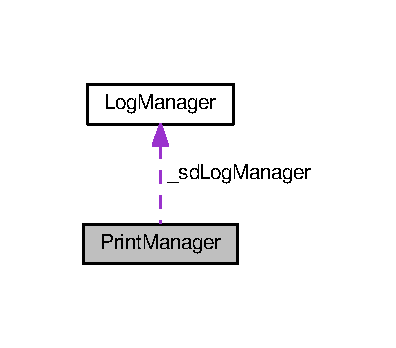
\includegraphics[width=190pt]{class_print_manager__coll__graph}
\end{center}
\end{figure}
\subsection*{Public Member Functions}
\begin{DoxyCompactItemize}
\item 
\hyperlink{class_print_manager_a587a22b1cc67696f71f5a85bfb130140}{Print\+Manager} (Hardware\+Serial $\ast$serial\+Port\+HW)
\item 
\hyperlink{class_print_manager_ac1212bb44b3c100bd67041d878977058}{Print\+Manager} (Software\+Serial $\ast$serial\+Port\+SW)
\item 
\hyperlink{class_print_manager_a5ac22dd7ed0f35b12cd2b7650e2c8501}{Print\+Manager} (Hardware\+Serial $\ast$serial\+Port\+HW, \hyperlink{class_log_manager}{Log\+Manager} $\ast$sd\+Log\+Manager)
\item 
\hyperlink{class_print_manager_ac1a82b54cdeaf43b3e78ed6eb18c9bc6}{Print\+Manager} (Software\+Serial $\ast$serial\+Port\+SW, \hyperlink{class_log_manager}{Log\+Manager} $\ast$sd\+Log\+Manager)
\item 
uint8\+\_\+t \hyperlink{class_print_manager_a65b6e94eb17c08725d307293c26922c6}{send\+Data} ()
\item 
void \hyperlink{class_print_manager_aef5dd6437e06e84de5a98c1466f5f074}{fast\+Value} (const char fmt, const double value)
\item 
void \hyperlink{class_print_manager_a27ea0c1977a54e1291d0be0fc0754f48}{add\+Value} (const char $\ast$fmt,...)
\item 
void \hyperlink{class_print_manager_a9a44c89a9752e1e1f63bc174ce675f90}{add\+Header} (const char $\ast$fmt,...)
\item 
void \hyperlink{class_print_manager_ae091788c5f4baa9df10fb290c67cb693}{fast\+Value} (const char $\ast$fmt,...)
\end{DoxyCompactItemize}
\subsection*{Protected Member Functions}
\begin{DoxyCompactItemize}
\item 
void \hyperlink{class_print_manager_abe73e179fbf7817ac2501663086efa6a}{make\+Header} ()
\item 
void \hyperlink{class_print_manager_aefa604ff2567aefd703c584cf530f581}{make\+Currently} ()
\end{DoxyCompactItemize}
\subsection*{Protected Attributes}
\begin{DoxyCompactItemize}
\item 
String \hyperlink{class_print_manager_a352c21440d4b8da910822603bbc6439d}{\+\_\+message\+Header} = \char`\"{}\{\char`\"{}
\item 
String \hyperlink{class_print_manager_a45a45bb347196bab8c3071cc5de6631a}{\+\_\+message\+Currently} = \char`\"{}\textbackslash{}\char`\"{}currently\textbackslash{}\char`\"{}\+: \{\char`\"{}
\item 
String \hyperlink{class_print_manager_ac499e04d25e84c7d7841d24c38a3bd47}{\+\_\+timezone} = \char`\"{}\textbackslash{}\char`\"{}Brazil/Brasília\textbackslash{}\char`\"{}\char`\"{}
\item 
uint8\+\_\+t \hyperlink{class_print_manager_ae1b8f767b738748027e0ac2a97f1be6c}{\+\_\+serial\+Port\+Type}
\item 
double \hyperlink{class_print_manager_a550ad6ba340af9c4f689b8e25bd420f3}{\+\_\+temp\+Value}
\item 
double \hyperlink{class_print_manager_a722d74baa1b0286c84b6d5181996ba2e}{\+\_\+latitude}
\item 
double \hyperlink{class_print_manager_a31a2a77dba86f3d99af5c6bd1d2baa4c}{\+\_\+longitude}
\item 
Hardware\+Serial $\ast$ \hyperlink{class_print_manager_a19cd58c07357e6142b92ed4598cda1bc}{\+\_\+serial\+Port\+HW}
\item 
Software\+Serial $\ast$ \hyperlink{class_print_manager_aa079f14838d51ffd18ac814323c3d177}{\+\_\+serial\+Port\+SW}
\item 
\hyperlink{class_log_manager}{Log\+Manager} $\ast$ \hyperlink{class_print_manager_a76f3172298d67da7428e55b2515aa030}{\+\_\+sd\+Log\+Manager}
\end{DoxyCompactItemize}


\subsection{Detailed Description}


Definition at line 15 of file Print\+Manager.\+hpp.



\subsection{Constructor \& Destructor Documentation}
\index{Print\+Manager@{Print\+Manager}!Print\+Manager@{Print\+Manager}}
\index{Print\+Manager@{Print\+Manager}!Print\+Manager@{Print\+Manager}}
\subsubsection[{\texorpdfstring{Print\+Manager(\+Hardware\+Serial $\ast$serial\+Port\+H\+W)}{PrintManager(HardwareSerial *serialPortHW)}}]{\setlength{\rightskip}{0pt plus 5cm}Print\+Manager\+::\+Print\+Manager (
\begin{DoxyParamCaption}
\item[{Hardware\+Serial $\ast$}]{serial\+Port\+HW}
\end{DoxyParamCaption}
)\hspace{0.3cm}{\ttfamily [inline]}}\hypertarget{class_print_manager_a587a22b1cc67696f71f5a85bfb130140}{}\label{class_print_manager_a587a22b1cc67696f71f5a85bfb130140}


Definition at line 17 of file Print\+Manager.\+hpp.

\index{Print\+Manager@{Print\+Manager}!Print\+Manager@{Print\+Manager}}
\index{Print\+Manager@{Print\+Manager}!Print\+Manager@{Print\+Manager}}
\subsubsection[{\texorpdfstring{Print\+Manager(\+Software\+Serial $\ast$serial\+Port\+S\+W)}{PrintManager(SoftwareSerial *serialPortSW)}}]{\setlength{\rightskip}{0pt plus 5cm}Print\+Manager\+::\+Print\+Manager (
\begin{DoxyParamCaption}
\item[{Software\+Serial $\ast$}]{serial\+Port\+SW}
\end{DoxyParamCaption}
)\hspace{0.3cm}{\ttfamily [inline]}}\hypertarget{class_print_manager_ac1212bb44b3c100bd67041d878977058}{}\label{class_print_manager_ac1212bb44b3c100bd67041d878977058}


Definition at line 23 of file Print\+Manager.\+hpp.

\index{Print\+Manager@{Print\+Manager}!Print\+Manager@{Print\+Manager}}
\index{Print\+Manager@{Print\+Manager}!Print\+Manager@{Print\+Manager}}
\subsubsection[{\texorpdfstring{Print\+Manager(\+Hardware\+Serial $\ast$serial\+Port\+H\+W, Log\+Manager $\ast$sd\+Log\+Manager)}{PrintManager(HardwareSerial *serialPortHW, LogManager *sdLogManager)}}]{\setlength{\rightskip}{0pt plus 5cm}Print\+Manager\+::\+Print\+Manager (
\begin{DoxyParamCaption}
\item[{Hardware\+Serial $\ast$}]{serial\+Port\+HW, }
\item[{{\bf Log\+Manager} $\ast$}]{sd\+Log\+Manager}
\end{DoxyParamCaption}
)\hspace{0.3cm}{\ttfamily [inline]}}\hypertarget{class_print_manager_a5ac22dd7ed0f35b12cd2b7650e2c8501}{}\label{class_print_manager_a5ac22dd7ed0f35b12cd2b7650e2c8501}


Definition at line 29 of file Print\+Manager.\+hpp.

\index{Print\+Manager@{Print\+Manager}!Print\+Manager@{Print\+Manager}}
\index{Print\+Manager@{Print\+Manager}!Print\+Manager@{Print\+Manager}}
\subsubsection[{\texorpdfstring{Print\+Manager(\+Software\+Serial $\ast$serial\+Port\+S\+W, Log\+Manager $\ast$sd\+Log\+Manager)}{PrintManager(SoftwareSerial *serialPortSW, LogManager *sdLogManager)}}]{\setlength{\rightskip}{0pt plus 5cm}Print\+Manager\+::\+Print\+Manager (
\begin{DoxyParamCaption}
\item[{Software\+Serial $\ast$}]{serial\+Port\+SW, }
\item[{{\bf Log\+Manager} $\ast$}]{sd\+Log\+Manager}
\end{DoxyParamCaption}
)\hspace{0.3cm}{\ttfamily [inline]}}\hypertarget{class_print_manager_ac1a82b54cdeaf43b3e78ed6eb18c9bc6}{}\label{class_print_manager_ac1a82b54cdeaf43b3e78ed6eb18c9bc6}


Definition at line 35 of file Print\+Manager.\+hpp.



\subsection{Member Function Documentation}
\index{Print\+Manager@{Print\+Manager}!add\+Header@{add\+Header}}
\index{add\+Header@{add\+Header}!Print\+Manager@{Print\+Manager}}
\subsubsection[{\texorpdfstring{add\+Header(const char $\ast$fmt,...)}{addHeader(const char *fmt,...)}}]{\setlength{\rightskip}{0pt plus 5cm}void Print\+Manager\+::add\+Header (
\begin{DoxyParamCaption}
\item[{const char $\ast$}]{fmt, }
\item[{}]{...}
\end{DoxyParamCaption}
)}\hypertarget{class_print_manager_a9a44c89a9752e1e1f63bc174ce675f90}{}\label{class_print_manager_a9a44c89a9752e1e1f63bc174ce675f90}


Definition at line 95 of file Print\+Manager.\+cpp.

\index{Print\+Manager@{Print\+Manager}!add\+Value@{add\+Value}}
\index{add\+Value@{add\+Value}!Print\+Manager@{Print\+Manager}}
\subsubsection[{\texorpdfstring{add\+Value(const char $\ast$fmt,...)}{addValue(const char *fmt,...)}}]{\setlength{\rightskip}{0pt plus 5cm}void Print\+Manager\+::add\+Value (
\begin{DoxyParamCaption}
\item[{const char $\ast$}]{fmt, }
\item[{}]{...}
\end{DoxyParamCaption}
)}\hypertarget{class_print_manager_a27ea0c1977a54e1291d0be0fc0754f48}{}\label{class_print_manager_a27ea0c1977a54e1291d0be0fc0754f48}


Definition at line 8 of file Print\+Manager.\+cpp.

\index{Print\+Manager@{Print\+Manager}!fast\+Value@{fast\+Value}}
\index{fast\+Value@{fast\+Value}!Print\+Manager@{Print\+Manager}}
\subsubsection[{\texorpdfstring{fast\+Value(const char fmt, const double value)}{fastValue(const char fmt, const double value)}}]{\setlength{\rightskip}{0pt plus 5cm}void Print\+Manager\+::fast\+Value (
\begin{DoxyParamCaption}
\item[{const char}]{fmt, }
\item[{const double}]{value}
\end{DoxyParamCaption}
)}\hypertarget{class_print_manager_aef5dd6437e06e84de5a98c1466f5f074}{}\label{class_print_manager_aef5dd6437e06e84de5a98c1466f5f074}


Definition at line 131 of file Print\+Manager.\+cpp.

\index{Print\+Manager@{Print\+Manager}!fast\+Value@{fast\+Value}}
\index{fast\+Value@{fast\+Value}!Print\+Manager@{Print\+Manager}}
\subsubsection[{\texorpdfstring{fast\+Value(const char $\ast$fmt,...)}{fastValue(const char *fmt,...)}}]{\setlength{\rightskip}{0pt plus 5cm}void Print\+Manager\+::fast\+Value (
\begin{DoxyParamCaption}
\item[{const char $\ast$}]{fmt, }
\item[{}]{...}
\end{DoxyParamCaption}
)}\hypertarget{class_print_manager_ae091788c5f4baa9df10fb290c67cb693}{}\label{class_print_manager_ae091788c5f4baa9df10fb290c67cb693}
\index{Print\+Manager@{Print\+Manager}!make\+Currently@{make\+Currently}}
\index{make\+Currently@{make\+Currently}!Print\+Manager@{Print\+Manager}}
\subsubsection[{\texorpdfstring{make\+Currently()}{makeCurrently()}}]{\setlength{\rightskip}{0pt plus 5cm}void Print\+Manager\+::make\+Currently (
\begin{DoxyParamCaption}
\item[{void}]{}
\end{DoxyParamCaption}
)\hspace{0.3cm}{\ttfamily [protected]}}\hypertarget{class_print_manager_aefa604ff2567aefd703c584cf530f581}{}\label{class_print_manager_aefa604ff2567aefd703c584cf530f581}


Definition at line 126 of file Print\+Manager.\+cpp.

\index{Print\+Manager@{Print\+Manager}!make\+Header@{make\+Header}}
\index{make\+Header@{make\+Header}!Print\+Manager@{Print\+Manager}}
\subsubsection[{\texorpdfstring{make\+Header()}{makeHeader()}}]{\setlength{\rightskip}{0pt plus 5cm}void Print\+Manager\+::make\+Header (
\begin{DoxyParamCaption}
\item[{void}]{}
\end{DoxyParamCaption}
)\hspace{0.3cm}{\ttfamily [protected]}}\hypertarget{class_print_manager_abe73e179fbf7817ac2501663086efa6a}{}\label{class_print_manager_abe73e179fbf7817ac2501663086efa6a}


Definition at line 116 of file Print\+Manager.\+cpp.

\index{Print\+Manager@{Print\+Manager}!send\+Data@{send\+Data}}
\index{send\+Data@{send\+Data}!Print\+Manager@{Print\+Manager}}
\subsubsection[{\texorpdfstring{send\+Data()}{sendData()}}]{\setlength{\rightskip}{0pt plus 5cm}uint8\+\_\+t Print\+Manager\+::send\+Data (
\begin{DoxyParamCaption}
{}
\end{DoxyParamCaption}
)}\hypertarget{class_print_manager_a65b6e94eb17c08725d307293c26922c6}{}\label{class_print_manager_a65b6e94eb17c08725d307293c26922c6}


Definition at line 137 of file Print\+Manager.\+cpp.



\subsection{Member Data Documentation}
\index{Print\+Manager@{Print\+Manager}!\+\_\+latitude@{\+\_\+latitude}}
\index{\+\_\+latitude@{\+\_\+latitude}!Print\+Manager@{Print\+Manager}}
\subsubsection[{\texorpdfstring{\+\_\+latitude}{_latitude}}]{\setlength{\rightskip}{0pt plus 5cm}double Print\+Manager\+::\+\_\+latitude\hspace{0.3cm}{\ttfamily [protected]}}\hypertarget{class_print_manager_a722d74baa1b0286c84b6d5181996ba2e}{}\label{class_print_manager_a722d74baa1b0286c84b6d5181996ba2e}


Definition at line 56 of file Print\+Manager.\+hpp.

\index{Print\+Manager@{Print\+Manager}!\+\_\+longitude@{\+\_\+longitude}}
\index{\+\_\+longitude@{\+\_\+longitude}!Print\+Manager@{Print\+Manager}}
\subsubsection[{\texorpdfstring{\+\_\+longitude}{_longitude}}]{\setlength{\rightskip}{0pt plus 5cm}double Print\+Manager\+::\+\_\+longitude\hspace{0.3cm}{\ttfamily [protected]}}\hypertarget{class_print_manager_a31a2a77dba86f3d99af5c6bd1d2baa4c}{}\label{class_print_manager_a31a2a77dba86f3d99af5c6bd1d2baa4c}


Definition at line 56 of file Print\+Manager.\+hpp.

\index{Print\+Manager@{Print\+Manager}!\+\_\+message\+Currently@{\+\_\+message\+Currently}}
\index{\+\_\+message\+Currently@{\+\_\+message\+Currently}!Print\+Manager@{Print\+Manager}}
\subsubsection[{\texorpdfstring{\+\_\+message\+Currently}{_messageCurrently}}]{\setlength{\rightskip}{0pt plus 5cm}String Print\+Manager\+::\+\_\+message\+Currently = \char`\"{}\textbackslash{}\char`\"{}currently\textbackslash{}\char`\"{}\+: \{\char`\"{}\hspace{0.3cm}{\ttfamily [protected]}}\hypertarget{class_print_manager_a45a45bb347196bab8c3071cc5de6631a}{}\label{class_print_manager_a45a45bb347196bab8c3071cc5de6631a}


Definition at line 53 of file Print\+Manager.\+hpp.

\index{Print\+Manager@{Print\+Manager}!\+\_\+message\+Header@{\+\_\+message\+Header}}
\index{\+\_\+message\+Header@{\+\_\+message\+Header}!Print\+Manager@{Print\+Manager}}
\subsubsection[{\texorpdfstring{\+\_\+message\+Header}{_messageHeader}}]{\setlength{\rightskip}{0pt plus 5cm}String Print\+Manager\+::\+\_\+message\+Header = \char`\"{}\{\char`\"{}\hspace{0.3cm}{\ttfamily [protected]}}\hypertarget{class_print_manager_a352c21440d4b8da910822603bbc6439d}{}\label{class_print_manager_a352c21440d4b8da910822603bbc6439d}


Definition at line 52 of file Print\+Manager.\+hpp.

\index{Print\+Manager@{Print\+Manager}!\+\_\+sd\+Log\+Manager@{\+\_\+sd\+Log\+Manager}}
\index{\+\_\+sd\+Log\+Manager@{\+\_\+sd\+Log\+Manager}!Print\+Manager@{Print\+Manager}}
\subsubsection[{\texorpdfstring{\+\_\+sd\+Log\+Manager}{_sdLogManager}}]{\setlength{\rightskip}{0pt plus 5cm}{\bf Log\+Manager}$\ast$ Print\+Manager\+::\+\_\+sd\+Log\+Manager\hspace{0.3cm}{\ttfamily [protected]}}\hypertarget{class_print_manager_a76f3172298d67da7428e55b2515aa030}{}\label{class_print_manager_a76f3172298d67da7428e55b2515aa030}


Definition at line 59 of file Print\+Manager.\+hpp.

\index{Print\+Manager@{Print\+Manager}!\+\_\+serial\+Port\+HW@{\+\_\+serial\+Port\+HW}}
\index{\+\_\+serial\+Port\+HW@{\+\_\+serial\+Port\+HW}!Print\+Manager@{Print\+Manager}}
\subsubsection[{\texorpdfstring{\+\_\+serial\+Port\+HW}{_serialPortHW}}]{\setlength{\rightskip}{0pt plus 5cm}Hardware\+Serial$\ast$ Print\+Manager\+::\+\_\+serial\+Port\+HW\hspace{0.3cm}{\ttfamily [protected]}}\hypertarget{class_print_manager_a19cd58c07357e6142b92ed4598cda1bc}{}\label{class_print_manager_a19cd58c07357e6142b92ed4598cda1bc}


Definition at line 57 of file Print\+Manager.\+hpp.

\index{Print\+Manager@{Print\+Manager}!\+\_\+serial\+Port\+SW@{\+\_\+serial\+Port\+SW}}
\index{\+\_\+serial\+Port\+SW@{\+\_\+serial\+Port\+SW}!Print\+Manager@{Print\+Manager}}
\subsubsection[{\texorpdfstring{\+\_\+serial\+Port\+SW}{_serialPortSW}}]{\setlength{\rightskip}{0pt plus 5cm}Software\+Serial$\ast$ Print\+Manager\+::\+\_\+serial\+Port\+SW\hspace{0.3cm}{\ttfamily [protected]}}\hypertarget{class_print_manager_aa079f14838d51ffd18ac814323c3d177}{}\label{class_print_manager_aa079f14838d51ffd18ac814323c3d177}


Definition at line 58 of file Print\+Manager.\+hpp.

\index{Print\+Manager@{Print\+Manager}!\+\_\+serial\+Port\+Type@{\+\_\+serial\+Port\+Type}}
\index{\+\_\+serial\+Port\+Type@{\+\_\+serial\+Port\+Type}!Print\+Manager@{Print\+Manager}}
\subsubsection[{\texorpdfstring{\+\_\+serial\+Port\+Type}{_serialPortType}}]{\setlength{\rightskip}{0pt plus 5cm}uint8\+\_\+t Print\+Manager\+::\+\_\+serial\+Port\+Type\hspace{0.3cm}{\ttfamily [protected]}}\hypertarget{class_print_manager_ae1b8f767b738748027e0ac2a97f1be6c}{}\label{class_print_manager_ae1b8f767b738748027e0ac2a97f1be6c}


Definition at line 55 of file Print\+Manager.\+hpp.

\index{Print\+Manager@{Print\+Manager}!\+\_\+temp\+Value@{\+\_\+temp\+Value}}
\index{\+\_\+temp\+Value@{\+\_\+temp\+Value}!Print\+Manager@{Print\+Manager}}
\subsubsection[{\texorpdfstring{\+\_\+temp\+Value}{_tempValue}}]{\setlength{\rightskip}{0pt plus 5cm}double Print\+Manager\+::\+\_\+temp\+Value\hspace{0.3cm}{\ttfamily [protected]}}\hypertarget{class_print_manager_a550ad6ba340af9c4f689b8e25bd420f3}{}\label{class_print_manager_a550ad6ba340af9c4f689b8e25bd420f3}


Definition at line 56 of file Print\+Manager.\+hpp.

\index{Print\+Manager@{Print\+Manager}!\+\_\+timezone@{\+\_\+timezone}}
\index{\+\_\+timezone@{\+\_\+timezone}!Print\+Manager@{Print\+Manager}}
\subsubsection[{\texorpdfstring{\+\_\+timezone}{_timezone}}]{\setlength{\rightskip}{0pt plus 5cm}String Print\+Manager\+::\+\_\+timezone = \char`\"{}\textbackslash{}\char`\"{}Brazil/Brasília\textbackslash{}\char`\"{}\char`\"{}\hspace{0.3cm}{\ttfamily [protected]}}\hypertarget{class_print_manager_ac499e04d25e84c7d7841d24c38a3bd47}{}\label{class_print_manager_ac499e04d25e84c7d7841d24c38a3bd47}


Definition at line 54 of file Print\+Manager.\+hpp.



The documentation for this class was generated from the following files\+:\begin{DoxyCompactItemize}
\item 
lib/\+Print\+Manager/src/\hyperlink{_print_manager_8hpp}{Print\+Manager.\+hpp}\item 
lib/\+Print\+Manager/src/\hyperlink{_print_manager_8cpp}{Print\+Manager.\+cpp}\end{DoxyCompactItemize}

\hypertarget{struct_raw_degrees}{}\section{Raw\+Degrees Struct Reference}
\label{struct_raw_degrees}\index{Raw\+Degrees@{Raw\+Degrees}}


{\ttfamily \#include $<$Tiny\+G\+P\+S++.\+h$>$}

\subsection*{Public Member Functions}
\begin{DoxyCompactItemize}
\item 
\hyperlink{struct_raw_degrees_a156d5ced092fa1473b9b669a29be3509}{Raw\+Degrees} ()
\end{DoxyCompactItemize}
\subsection*{Public Attributes}
\begin{DoxyCompactItemize}
\item 
uint16\+\_\+t \hyperlink{struct_raw_degrees_a11831d9220f303bd716d9412af28e84e}{deg}
\item 
uint32\+\_\+t \hyperlink{struct_raw_degrees_a13564009c60e20dbf03b158114d1c0e2}{billionths}
\item 
bool \hyperlink{struct_raw_degrees_a39c31d2d0332155a4d2c975cec0a796f}{negative}
\end{DoxyCompactItemize}


\subsection{Detailed Description}


Definition at line 43 of file Tiny\+G\+P\+S++.\+h.



\subsection{Constructor \& Destructor Documentation}
\index{Raw\+Degrees@{Raw\+Degrees}!Raw\+Degrees@{Raw\+Degrees}}
\index{Raw\+Degrees@{Raw\+Degrees}!Raw\+Degrees@{Raw\+Degrees}}
\subsubsection[{\texorpdfstring{Raw\+Degrees()}{RawDegrees()}}]{\setlength{\rightskip}{0pt plus 5cm}Raw\+Degrees\+::\+Raw\+Degrees (
\begin{DoxyParamCaption}
{}
\end{DoxyParamCaption}
)\hspace{0.3cm}{\ttfamily [inline]}}\hypertarget{struct_raw_degrees_a156d5ced092fa1473b9b669a29be3509}{}\label{struct_raw_degrees_a156d5ced092fa1473b9b669a29be3509}


Definition at line 49 of file Tiny\+G\+P\+S++.\+h.



\subsection{Member Data Documentation}
\index{Raw\+Degrees@{Raw\+Degrees}!billionths@{billionths}}
\index{billionths@{billionths}!Raw\+Degrees@{Raw\+Degrees}}
\subsubsection[{\texorpdfstring{billionths}{billionths}}]{\setlength{\rightskip}{0pt plus 5cm}uint32\+\_\+t Raw\+Degrees\+::billionths}\hypertarget{struct_raw_degrees_a13564009c60e20dbf03b158114d1c0e2}{}\label{struct_raw_degrees_a13564009c60e20dbf03b158114d1c0e2}


Definition at line 46 of file Tiny\+G\+P\+S++.\+h.

\index{Raw\+Degrees@{Raw\+Degrees}!deg@{deg}}
\index{deg@{deg}!Raw\+Degrees@{Raw\+Degrees}}
\subsubsection[{\texorpdfstring{deg}{deg}}]{\setlength{\rightskip}{0pt plus 5cm}uint16\+\_\+t Raw\+Degrees\+::deg}\hypertarget{struct_raw_degrees_a11831d9220f303bd716d9412af28e84e}{}\label{struct_raw_degrees_a11831d9220f303bd716d9412af28e84e}


Definition at line 45 of file Tiny\+G\+P\+S++.\+h.

\index{Raw\+Degrees@{Raw\+Degrees}!negative@{negative}}
\index{negative@{negative}!Raw\+Degrees@{Raw\+Degrees}}
\subsubsection[{\texorpdfstring{negative}{negative}}]{\setlength{\rightskip}{0pt plus 5cm}bool Raw\+Degrees\+::negative}\hypertarget{struct_raw_degrees_a39c31d2d0332155a4d2c975cec0a796f}{}\label{struct_raw_degrees_a39c31d2d0332155a4d2c975cec0a796f}


Definition at line 47 of file Tiny\+G\+P\+S++.\+h.



The documentation for this struct was generated from the following file\+:\begin{DoxyCompactItemize}
\item 
lib/\+Tiny\+G\+P\+S\+Plus/\hyperlink{_tiny_g_p_s_09_09_8h}{Tiny\+G\+P\+S++.\+h}\end{DoxyCompactItemize}

\hypertarget{class_rtc_date_time}{}\section{Rtc\+Date\+Time Class Reference}
\label{class_rtc_date_time}\index{Rtc\+Date\+Time@{Rtc\+Date\+Time}}


{\ttfamily \#include $<$Rtc\+Date\+Time.\+h$>$}

\subsection*{Public Member Functions}
\begin{DoxyCompactItemize}
\item 
\hyperlink{class_rtc_date_time_ae874891e1f436469ed4087483447c882}{Rtc\+Date\+Time} (uint32\+\_\+t seconds\+From2000=0)
\item 
\hyperlink{class_rtc_date_time_a547de741c4dc29d7097ed6c58b7c7cd3}{Rtc\+Date\+Time} (uint16\+\_\+t year, uint8\+\_\+t month, uint8\+\_\+t day\+Of\+Month, uint8\+\_\+t hour, uint8\+\_\+t minute, uint8\+\_\+t second)
\item 
\hyperlink{class_rtc_date_time_a7f00c81c8dbb3572062018357f17b0e4}{Rtc\+Date\+Time} (const char $\ast$date, const char $\ast$time)
\item 
uint16\+\_\+t \hyperlink{class_rtc_date_time_a9e09852c29989b3d5e1301138be34a59}{Year} () const 
\item 
uint8\+\_\+t \hyperlink{class_rtc_date_time_a581aafb10357287a936d3d8be95c7035}{Month} () const 
\item 
uint8\+\_\+t \hyperlink{class_rtc_date_time_a179b27f370273e72037fbb425733ae13}{Day} () const 
\item 
uint8\+\_\+t \hyperlink{class_rtc_date_time_a6d06a178cfd394f5c4701a45e0d903ef}{Hour} () const 
\item 
uint8\+\_\+t \hyperlink{class_rtc_date_time_abd88320abfda5eb9962ef1bbdcb294bc}{Minute} () const 
\item 
uint8\+\_\+t \hyperlink{class_rtc_date_time_a7323ffadc8c2539ed296c62e1dbd6767}{Second} () const 
\item 
uint8\+\_\+t \hyperlink{class_rtc_date_time_a39c9b97eab71d7da5dc1fb2df308e756}{Day\+Of\+Week} () const 
\item 
uint32\+\_\+t \hyperlink{class_rtc_date_time_a51cc5ad5b4667fbce601289004c0a477}{Total\+Seconds} () const 
\item 
uint64\+\_\+t \hyperlink{class_rtc_date_time_a513bd36f76c7f4a6715c2d74a94e868a}{Total\+Seconds64} () const 
\item 
void \hyperlink{class_rtc_date_time_a6c43d51a9bd1a004e4d2a3eb1a8da84e}{operator+=} (uint32\+\_\+t seconds)
\item 
\hyperlink{class_rtc_date_time_af12e82c0f9cbe28d81ddb78e6316e0ee}{operator uint32\+\_\+t} () const 
\item 
uint32\+\_\+t \hyperlink{class_rtc_date_time_a77286613a3bbdda951a479158d53e53b}{Epoch32\+Time} () const 
\item 
void \hyperlink{class_rtc_date_time_afeb3551f82aa838fdb6347dc73c1f8e4}{Init\+With\+Epoch32\+Time} (uint32\+\_\+t time)
\item 
uint64\+\_\+t \hyperlink{class_rtc_date_time_a2ebb0cba0b82274a166daa618b4213cb}{Epoch64\+Time} () const 
\item 
void \hyperlink{class_rtc_date_time_a23fa488b500d4968a4619093005e5212}{Init\+With\+Epoch64\+Time} (uint64\+\_\+t time)
\end{DoxyCompactItemize}
\subsection*{Protected Member Functions}
\begin{DoxyCompactItemize}
\item 
{\footnotesize template$<$typename T $>$ }\\void \hyperlink{class_rtc_date_time_a60b21b4d2186c7daf8ed94a750e10f3a}{\+\_\+init\+With\+Seconds\+From2000} (T seconds\+From2000)
\end{DoxyCompactItemize}
\subsection*{Protected Attributes}
\begin{DoxyCompactItemize}
\item 
uint8\+\_\+t \hyperlink{class_rtc_date_time_a782f920fa91c813d1f34116f8ef58e17}{\+\_\+year\+From2000}
\item 
uint8\+\_\+t \hyperlink{class_rtc_date_time_ac330113b94c1bc110ad7dbc3a263f03a}{\+\_\+month}
\item 
uint8\+\_\+t \hyperlink{class_rtc_date_time_a12da2c12bb874dd069e092f9998c0e0c}{\+\_\+day\+Of\+Month}
\item 
uint8\+\_\+t \hyperlink{class_rtc_date_time_a93fcc560a087734a015cf63477708a78}{\+\_\+hour}
\item 
uint8\+\_\+t \hyperlink{class_rtc_date_time_a9f29cd580a5c8a60212cb96a553865cf}{\+\_\+minute}
\item 
uint8\+\_\+t \hyperlink{class_rtc_date_time_ad3c0899907fa14a51be81be3122d0a80}{\+\_\+second}
\end{DoxyCompactItemize}


\subsection{Detailed Description}


Definition at line 10 of file Rtc\+Date\+Time.\+h.



\subsection{Constructor \& Destructor Documentation}
\index{Rtc\+Date\+Time@{Rtc\+Date\+Time}!Rtc\+Date\+Time@{Rtc\+Date\+Time}}
\index{Rtc\+Date\+Time@{Rtc\+Date\+Time}!Rtc\+Date\+Time@{Rtc\+Date\+Time}}
\subsubsection[{\texorpdfstring{Rtc\+Date\+Time(uint32\+\_\+t seconds\+From2000=0)}{RtcDateTime(uint32_t secondsFrom2000=0)}}]{\setlength{\rightskip}{0pt plus 5cm}Rtc\+Date\+Time\+::\+Rtc\+Date\+Time (
\begin{DoxyParamCaption}
\item[{uint32\+\_\+t}]{seconds\+From2000 = {\ttfamily 0}}
\end{DoxyParamCaption}
)}\hypertarget{class_rtc_date_time_ae874891e1f436469ed4087483447c882}{}\label{class_rtc_date_time_ae874891e1f436469ed4087483447c882}


Definition at line 14 of file Rtc\+Date\+Time.\+cpp.

\index{Rtc\+Date\+Time@{Rtc\+Date\+Time}!Rtc\+Date\+Time@{Rtc\+Date\+Time}}
\index{Rtc\+Date\+Time@{Rtc\+Date\+Time}!Rtc\+Date\+Time@{Rtc\+Date\+Time}}
\subsubsection[{\texorpdfstring{Rtc\+Date\+Time(uint16\+\_\+t year, uint8\+\_\+t month, uint8\+\_\+t day\+Of\+Month, uint8\+\_\+t hour, uint8\+\_\+t minute, uint8\+\_\+t second)}{RtcDateTime(uint16_t year, uint8_t month, uint8_t dayOfMonth, uint8_t hour, uint8_t minute, uint8_t second)}}]{\setlength{\rightskip}{0pt plus 5cm}Rtc\+Date\+Time\+::\+Rtc\+Date\+Time (
\begin{DoxyParamCaption}
\item[{uint16\+\_\+t}]{year, }
\item[{uint8\+\_\+t}]{month, }
\item[{uint8\+\_\+t}]{day\+Of\+Month, }
\item[{uint8\+\_\+t}]{hour, }
\item[{uint8\+\_\+t}]{minute, }
\item[{uint8\+\_\+t}]{second}
\end{DoxyParamCaption}
)\hspace{0.3cm}{\ttfamily [inline]}}\hypertarget{class_rtc_date_time_a547de741c4dc29d7097ed6c58b7c7cd3}{}\label{class_rtc_date_time_a547de741c4dc29d7097ed6c58b7c7cd3}


Definition at line 14 of file Rtc\+Date\+Time.\+h.

\index{Rtc\+Date\+Time@{Rtc\+Date\+Time}!Rtc\+Date\+Time@{Rtc\+Date\+Time}}
\index{Rtc\+Date\+Time@{Rtc\+Date\+Time}!Rtc\+Date\+Time@{Rtc\+Date\+Time}}
\subsubsection[{\texorpdfstring{Rtc\+Date\+Time(const char $\ast$date, const char $\ast$time)}{RtcDateTime(const char *date, const char *time)}}]{\setlength{\rightskip}{0pt plus 5cm}Rtc\+Date\+Time\+::\+Rtc\+Date\+Time (
\begin{DoxyParamCaption}
\item[{const char $\ast$}]{date, }
\item[{const char $\ast$}]{time}
\end{DoxyParamCaption}
)}\hypertarget{class_rtc_date_time_a7f00c81c8dbb3572062018357f17b0e4}{}\label{class_rtc_date_time_a7f00c81c8dbb3572062018357f17b0e4}


Definition at line 40 of file Rtc\+Date\+Time.\+cpp.



\subsection{Member Function Documentation}
\index{Rtc\+Date\+Time@{Rtc\+Date\+Time}!\+\_\+init\+With\+Seconds\+From2000@{\+\_\+init\+With\+Seconds\+From2000}}
\index{\+\_\+init\+With\+Seconds\+From2000@{\+\_\+init\+With\+Seconds\+From2000}!Rtc\+Date\+Time@{Rtc\+Date\+Time}}
\subsubsection[{\texorpdfstring{\+\_\+init\+With\+Seconds\+From2000(\+T seconds\+From2000)}{_initWithSecondsFrom2000(T secondsFrom2000)}}]{\setlength{\rightskip}{0pt plus 5cm}template$<$typename T $>$ void Rtc\+Date\+Time\+::\+\_\+init\+With\+Seconds\+From2000 (
\begin{DoxyParamCaption}
\item[{T}]{seconds\+From2000}
\end{DoxyParamCaption}
)\hspace{0.3cm}{\ttfamily [inline]}, {\ttfamily [protected]}}\hypertarget{class_rtc_date_time_a60b21b4d2186c7daf8ed94a750e10f3a}{}\label{class_rtc_date_time_a60b21b4d2186c7daf8ed94a750e10f3a}


Definition at line 103 of file Rtc\+Date\+Time.\+h.

\index{Rtc\+Date\+Time@{Rtc\+Date\+Time}!Day@{Day}}
\index{Day@{Day}!Rtc\+Date\+Time@{Rtc\+Date\+Time}}
\subsubsection[{\texorpdfstring{Day() const }{Day() const }}]{\setlength{\rightskip}{0pt plus 5cm}uint8\+\_\+t Rtc\+Date\+Time\+::\+Day (
\begin{DoxyParamCaption}
{}
\end{DoxyParamCaption}
) const\hspace{0.3cm}{\ttfamily [inline]}}\hypertarget{class_rtc_date_time_a179b27f370273e72037fbb425733ae13}{}\label{class_rtc_date_time_a179b27f370273e72037fbb425733ae13}


Definition at line 40 of file Rtc\+Date\+Time.\+h.

\index{Rtc\+Date\+Time@{Rtc\+Date\+Time}!Day\+Of\+Week@{Day\+Of\+Week}}
\index{Day\+Of\+Week@{Day\+Of\+Week}!Rtc\+Date\+Time@{Rtc\+Date\+Time}}
\subsubsection[{\texorpdfstring{Day\+Of\+Week() const }{DayOfWeek() const }}]{\setlength{\rightskip}{0pt plus 5cm}uint8\+\_\+t Rtc\+Date\+Time\+::\+Day\+Of\+Week (
\begin{DoxyParamCaption}
{}
\end{DoxyParamCaption}
) const}\hypertarget{class_rtc_date_time_a39c9b97eab71d7da5dc1fb2df308e756}{}\label{class_rtc_date_time_a39c9b97eab71d7da5dc1fb2df308e756}


Definition at line 102 of file Rtc\+Date\+Time.\+cpp.

\index{Rtc\+Date\+Time@{Rtc\+Date\+Time}!Epoch32\+Time@{Epoch32\+Time}}
\index{Epoch32\+Time@{Epoch32\+Time}!Rtc\+Date\+Time@{Rtc\+Date\+Time}}
\subsubsection[{\texorpdfstring{Epoch32\+Time() const }{Epoch32Time() const }}]{\setlength{\rightskip}{0pt plus 5cm}uint32\+\_\+t Rtc\+Date\+Time\+::\+Epoch32\+Time (
\begin{DoxyParamCaption}
{}
\end{DoxyParamCaption}
) const\hspace{0.3cm}{\ttfamily [inline]}}\hypertarget{class_rtc_date_time_a77286613a3bbdda951a479158d53e53b}{}\label{class_rtc_date_time_a77286613a3bbdda951a479158d53e53b}


Definition at line 76 of file Rtc\+Date\+Time.\+h.

\index{Rtc\+Date\+Time@{Rtc\+Date\+Time}!Epoch64\+Time@{Epoch64\+Time}}
\index{Epoch64\+Time@{Epoch64\+Time}!Rtc\+Date\+Time@{Rtc\+Date\+Time}}
\subsubsection[{\texorpdfstring{Epoch64\+Time() const }{Epoch64Time() const }}]{\setlength{\rightskip}{0pt plus 5cm}uint64\+\_\+t Rtc\+Date\+Time\+::\+Epoch64\+Time (
\begin{DoxyParamCaption}
{}
\end{DoxyParamCaption}
) const\hspace{0.3cm}{\ttfamily [inline]}}\hypertarget{class_rtc_date_time_a2ebb0cba0b82274a166daa618b4213cb}{}\label{class_rtc_date_time_a2ebb0cba0b82274a166daa618b4213cb}


Definition at line 86 of file Rtc\+Date\+Time.\+h.

\index{Rtc\+Date\+Time@{Rtc\+Date\+Time}!Hour@{Hour}}
\index{Hour@{Hour}!Rtc\+Date\+Time@{Rtc\+Date\+Time}}
\subsubsection[{\texorpdfstring{Hour() const }{Hour() const }}]{\setlength{\rightskip}{0pt plus 5cm}uint8\+\_\+t Rtc\+Date\+Time\+::\+Hour (
\begin{DoxyParamCaption}
{}
\end{DoxyParamCaption}
) const\hspace{0.3cm}{\ttfamily [inline]}}\hypertarget{class_rtc_date_time_a6d06a178cfd394f5c4701a45e0d903ef}{}\label{class_rtc_date_time_a6d06a178cfd394f5c4701a45e0d903ef}


Definition at line 44 of file Rtc\+Date\+Time.\+h.

\index{Rtc\+Date\+Time@{Rtc\+Date\+Time}!Init\+With\+Epoch32\+Time@{Init\+With\+Epoch32\+Time}}
\index{Init\+With\+Epoch32\+Time@{Init\+With\+Epoch32\+Time}!Rtc\+Date\+Time@{Rtc\+Date\+Time}}
\subsubsection[{\texorpdfstring{Init\+With\+Epoch32\+Time(uint32\+\_\+t time)}{InitWithEpoch32Time(uint32_t time)}}]{\setlength{\rightskip}{0pt plus 5cm}void Rtc\+Date\+Time\+::\+Init\+With\+Epoch32\+Time (
\begin{DoxyParamCaption}
\item[{uint32\+\_\+t}]{time}
\end{DoxyParamCaption}
)\hspace{0.3cm}{\ttfamily [inline]}}\hypertarget{class_rtc_date_time_afeb3551f82aa838fdb6347dc73c1f8e4}{}\label{class_rtc_date_time_afeb3551f82aa838fdb6347dc73c1f8e4}


Definition at line 80 of file Rtc\+Date\+Time.\+h.

\index{Rtc\+Date\+Time@{Rtc\+Date\+Time}!Init\+With\+Epoch64\+Time@{Init\+With\+Epoch64\+Time}}
\index{Init\+With\+Epoch64\+Time@{Init\+With\+Epoch64\+Time}!Rtc\+Date\+Time@{Rtc\+Date\+Time}}
\subsubsection[{\texorpdfstring{Init\+With\+Epoch64\+Time(uint64\+\_\+t time)}{InitWithEpoch64Time(uint64_t time)}}]{\setlength{\rightskip}{0pt plus 5cm}void Rtc\+Date\+Time\+::\+Init\+With\+Epoch64\+Time (
\begin{DoxyParamCaption}
\item[{uint64\+\_\+t}]{time}
\end{DoxyParamCaption}
)\hspace{0.3cm}{\ttfamily [inline]}}\hypertarget{class_rtc_date_time_a23fa488b500d4968a4619093005e5212}{}\label{class_rtc_date_time_a23fa488b500d4968a4619093005e5212}


Definition at line 90 of file Rtc\+Date\+Time.\+h.

\index{Rtc\+Date\+Time@{Rtc\+Date\+Time}!Minute@{Minute}}
\index{Minute@{Minute}!Rtc\+Date\+Time@{Rtc\+Date\+Time}}
\subsubsection[{\texorpdfstring{Minute() const }{Minute() const }}]{\setlength{\rightskip}{0pt plus 5cm}uint8\+\_\+t Rtc\+Date\+Time\+::\+Minute (
\begin{DoxyParamCaption}
{}
\end{DoxyParamCaption}
) const\hspace{0.3cm}{\ttfamily [inline]}}\hypertarget{class_rtc_date_time_abd88320abfda5eb9962ef1bbdcb294bc}{}\label{class_rtc_date_time_abd88320abfda5eb9962ef1bbdcb294bc}


Definition at line 48 of file Rtc\+Date\+Time.\+h.

\index{Rtc\+Date\+Time@{Rtc\+Date\+Time}!Month@{Month}}
\index{Month@{Month}!Rtc\+Date\+Time@{Rtc\+Date\+Time}}
\subsubsection[{\texorpdfstring{Month() const }{Month() const }}]{\setlength{\rightskip}{0pt plus 5cm}uint8\+\_\+t Rtc\+Date\+Time\+::\+Month (
\begin{DoxyParamCaption}
{}
\end{DoxyParamCaption}
) const\hspace{0.3cm}{\ttfamily [inline]}}\hypertarget{class_rtc_date_time_a581aafb10357287a936d3d8be95c7035}{}\label{class_rtc_date_time_a581aafb10357287a936d3d8be95c7035}


Definition at line 36 of file Rtc\+Date\+Time.\+h.

\index{Rtc\+Date\+Time@{Rtc\+Date\+Time}!operator uint32\+\_\+t@{operator uint32\+\_\+t}}
\index{operator uint32\+\_\+t@{operator uint32\+\_\+t}!Rtc\+Date\+Time@{Rtc\+Date\+Time}}
\subsubsection[{\texorpdfstring{operator uint32\+\_\+t() const }{operator uint32_t() const }}]{\setlength{\rightskip}{0pt plus 5cm}Rtc\+Date\+Time\+::operator uint32\+\_\+t (
\begin{DoxyParamCaption}
{}
\end{DoxyParamCaption}
) const\hspace{0.3cm}{\ttfamily [inline]}}\hypertarget{class_rtc_date_time_af12e82c0f9cbe28d81ddb78e6316e0ee}{}\label{class_rtc_date_time_af12e82c0f9cbe28d81ddb78e6316e0ee}


Definition at line 70 of file Rtc\+Date\+Time.\+h.

\index{Rtc\+Date\+Time@{Rtc\+Date\+Time}!operator+=@{operator+=}}
\index{operator+=@{operator+=}!Rtc\+Date\+Time@{Rtc\+Date\+Time}}
\subsubsection[{\texorpdfstring{operator+=(uint32\+\_\+t seconds)}{operator+=(uint32_t seconds)}}]{\setlength{\rightskip}{0pt plus 5cm}void Rtc\+Date\+Time\+::operator+= (
\begin{DoxyParamCaption}
\item[{uint32\+\_\+t}]{seconds}
\end{DoxyParamCaption}
)\hspace{0.3cm}{\ttfamily [inline]}}\hypertarget{class_rtc_date_time_a6c43d51a9bd1a004e4d2a3eb1a8da84e}{}\label{class_rtc_date_time_a6c43d51a9bd1a004e4d2a3eb1a8da84e}


Definition at line 63 of file Rtc\+Date\+Time.\+h.

\index{Rtc\+Date\+Time@{Rtc\+Date\+Time}!Second@{Second}}
\index{Second@{Second}!Rtc\+Date\+Time@{Rtc\+Date\+Time}}
\subsubsection[{\texorpdfstring{Second() const }{Second() const }}]{\setlength{\rightskip}{0pt plus 5cm}uint8\+\_\+t Rtc\+Date\+Time\+::\+Second (
\begin{DoxyParamCaption}
{}
\end{DoxyParamCaption}
) const\hspace{0.3cm}{\ttfamily [inline]}}\hypertarget{class_rtc_date_time_a7323ffadc8c2539ed296c62e1dbd6767}{}\label{class_rtc_date_time_a7323ffadc8c2539ed296c62e1dbd6767}


Definition at line 52 of file Rtc\+Date\+Time.\+h.

\index{Rtc\+Date\+Time@{Rtc\+Date\+Time}!Total\+Seconds@{Total\+Seconds}}
\index{Total\+Seconds@{Total\+Seconds}!Rtc\+Date\+Time@{Rtc\+Date\+Time}}
\subsubsection[{\texorpdfstring{Total\+Seconds() const }{TotalSeconds() const }}]{\setlength{\rightskip}{0pt plus 5cm}uint32\+\_\+t Rtc\+Date\+Time\+::\+Total\+Seconds (
\begin{DoxyParamCaption}
{}
\end{DoxyParamCaption}
) const}\hypertarget{class_rtc_date_time_a51cc5ad5b4667fbce601289004c0a477}{}\label{class_rtc_date_time_a51cc5ad5b4667fbce601289004c0a477}


Definition at line 108 of file Rtc\+Date\+Time.\+cpp.

\index{Rtc\+Date\+Time@{Rtc\+Date\+Time}!Total\+Seconds64@{Total\+Seconds64}}
\index{Total\+Seconds64@{Total\+Seconds64}!Rtc\+Date\+Time@{Rtc\+Date\+Time}}
\subsubsection[{\texorpdfstring{Total\+Seconds64() const }{TotalSeconds64() const }}]{\setlength{\rightskip}{0pt plus 5cm}uint64\+\_\+t Rtc\+Date\+Time\+::\+Total\+Seconds64 (
\begin{DoxyParamCaption}
{}
\end{DoxyParamCaption}
) const}\hypertarget{class_rtc_date_time_a513bd36f76c7f4a6715c2d74a94e868a}{}\label{class_rtc_date_time_a513bd36f76c7f4a6715c2d74a94e868a}


Definition at line 114 of file Rtc\+Date\+Time.\+cpp.

\index{Rtc\+Date\+Time@{Rtc\+Date\+Time}!Year@{Year}}
\index{Year@{Year}!Rtc\+Date\+Time@{Rtc\+Date\+Time}}
\subsubsection[{\texorpdfstring{Year() const }{Year() const }}]{\setlength{\rightskip}{0pt plus 5cm}uint16\+\_\+t Rtc\+Date\+Time\+::\+Year (
\begin{DoxyParamCaption}
{}
\end{DoxyParamCaption}
) const\hspace{0.3cm}{\ttfamily [inline]}}\hypertarget{class_rtc_date_time_a9e09852c29989b3d5e1301138be34a59}{}\label{class_rtc_date_time_a9e09852c29989b3d5e1301138be34a59}


Definition at line 32 of file Rtc\+Date\+Time.\+h.



\subsection{Member Data Documentation}
\index{Rtc\+Date\+Time@{Rtc\+Date\+Time}!\+\_\+day\+Of\+Month@{\+\_\+day\+Of\+Month}}
\index{\+\_\+day\+Of\+Month@{\+\_\+day\+Of\+Month}!Rtc\+Date\+Time@{Rtc\+Date\+Time}}
\subsubsection[{\texorpdfstring{\+\_\+day\+Of\+Month}{_dayOfMonth}}]{\setlength{\rightskip}{0pt plus 5cm}uint8\+\_\+t Rtc\+Date\+Time\+::\+\_\+day\+Of\+Month\hspace{0.3cm}{\ttfamily [protected]}}\hypertarget{class_rtc_date_time_a12da2c12bb874dd069e092f9998c0e0c}{}\label{class_rtc_date_time_a12da2c12bb874dd069e092f9998c0e0c}


Definition at line 98 of file Rtc\+Date\+Time.\+h.

\index{Rtc\+Date\+Time@{Rtc\+Date\+Time}!\+\_\+hour@{\+\_\+hour}}
\index{\+\_\+hour@{\+\_\+hour}!Rtc\+Date\+Time@{Rtc\+Date\+Time}}
\subsubsection[{\texorpdfstring{\+\_\+hour}{_hour}}]{\setlength{\rightskip}{0pt plus 5cm}uint8\+\_\+t Rtc\+Date\+Time\+::\+\_\+hour\hspace{0.3cm}{\ttfamily [protected]}}\hypertarget{class_rtc_date_time_a93fcc560a087734a015cf63477708a78}{}\label{class_rtc_date_time_a93fcc560a087734a015cf63477708a78}


Definition at line 99 of file Rtc\+Date\+Time.\+h.

\index{Rtc\+Date\+Time@{Rtc\+Date\+Time}!\+\_\+minute@{\+\_\+minute}}
\index{\+\_\+minute@{\+\_\+minute}!Rtc\+Date\+Time@{Rtc\+Date\+Time}}
\subsubsection[{\texorpdfstring{\+\_\+minute}{_minute}}]{\setlength{\rightskip}{0pt plus 5cm}uint8\+\_\+t Rtc\+Date\+Time\+::\+\_\+minute\hspace{0.3cm}{\ttfamily [protected]}}\hypertarget{class_rtc_date_time_a9f29cd580a5c8a60212cb96a553865cf}{}\label{class_rtc_date_time_a9f29cd580a5c8a60212cb96a553865cf}


Definition at line 100 of file Rtc\+Date\+Time.\+h.

\index{Rtc\+Date\+Time@{Rtc\+Date\+Time}!\+\_\+month@{\+\_\+month}}
\index{\+\_\+month@{\+\_\+month}!Rtc\+Date\+Time@{Rtc\+Date\+Time}}
\subsubsection[{\texorpdfstring{\+\_\+month}{_month}}]{\setlength{\rightskip}{0pt plus 5cm}uint8\+\_\+t Rtc\+Date\+Time\+::\+\_\+month\hspace{0.3cm}{\ttfamily [protected]}}\hypertarget{class_rtc_date_time_ac330113b94c1bc110ad7dbc3a263f03a}{}\label{class_rtc_date_time_ac330113b94c1bc110ad7dbc3a263f03a}


Definition at line 97 of file Rtc\+Date\+Time.\+h.

\index{Rtc\+Date\+Time@{Rtc\+Date\+Time}!\+\_\+second@{\+\_\+second}}
\index{\+\_\+second@{\+\_\+second}!Rtc\+Date\+Time@{Rtc\+Date\+Time}}
\subsubsection[{\texorpdfstring{\+\_\+second}{_second}}]{\setlength{\rightskip}{0pt plus 5cm}uint8\+\_\+t Rtc\+Date\+Time\+::\+\_\+second\hspace{0.3cm}{\ttfamily [protected]}}\hypertarget{class_rtc_date_time_ad3c0899907fa14a51be81be3122d0a80}{}\label{class_rtc_date_time_ad3c0899907fa14a51be81be3122d0a80}


Definition at line 101 of file Rtc\+Date\+Time.\+h.

\index{Rtc\+Date\+Time@{Rtc\+Date\+Time}!\+\_\+year\+From2000@{\+\_\+year\+From2000}}
\index{\+\_\+year\+From2000@{\+\_\+year\+From2000}!Rtc\+Date\+Time@{Rtc\+Date\+Time}}
\subsubsection[{\texorpdfstring{\+\_\+year\+From2000}{_yearFrom2000}}]{\setlength{\rightskip}{0pt plus 5cm}uint8\+\_\+t Rtc\+Date\+Time\+::\+\_\+year\+From2000\hspace{0.3cm}{\ttfamily [protected]}}\hypertarget{class_rtc_date_time_a782f920fa91c813d1f34116f8ef58e17}{}\label{class_rtc_date_time_a782f920fa91c813d1f34116f8ef58e17}


Definition at line 96 of file Rtc\+Date\+Time.\+h.



The documentation for this class was generated from the following files\+:\begin{DoxyCompactItemize}
\item 
lib/\+R\+T\+C/src/\hyperlink{_rtc_date_time_8h}{Rtc\+Date\+Time.\+h}\item 
lib/\+R\+T\+C/src/\hyperlink{_rtc_date_time_8cpp}{Rtc\+Date\+Time.\+cpp}\end{DoxyCompactItemize}

\hypertarget{class_rtc_d_s1307}{}\section{Rtc\+D\+S1307$<$ T\+\_\+\+W\+I\+R\+E\+\_\+\+M\+E\+T\+H\+OD $>$ Class Template Reference}
\label{class_rtc_d_s1307}\index{Rtc\+D\+S1307$<$ T\+\_\+\+W\+I\+R\+E\+\_\+\+M\+E\+T\+H\+O\+D $>$@{Rtc\+D\+S1307$<$ T\+\_\+\+W\+I\+R\+E\+\_\+\+M\+E\+T\+H\+O\+D $>$}}


{\ttfamily \#include $<$Rtc\+D\+S1307.\+h$>$}

\subsection*{Public Member Functions}
\begin{DoxyCompactItemize}
\item 
\hyperlink{class_rtc_d_s1307_a3cc15257ca35d2016ea9cd952fce19fc}{Rtc\+D\+S1307} (T\+\_\+\+W\+I\+R\+E\+\_\+\+M\+E\+T\+H\+OD \&wire)
\item 
void \hyperlink{class_rtc_d_s1307_a7c9ca31bbee2bf317f9f7d0858670f77}{Begin} ()
\item 
bool \hyperlink{class_rtc_d_s1307_a59c23764273ce04cd12c7b24e05d6aad}{Is\+Date\+Time\+Valid} ()
\item 
bool \hyperlink{class_rtc_d_s1307_abef3ed4e0898645e62d293a5d8e3c8db}{Get\+Is\+Running} ()
\item 
void \hyperlink{class_rtc_d_s1307_a48280782960f2d3d6bfcc14db3382475}{Set\+Is\+Running} (bool is\+Running)
\item 
void \hyperlink{class_rtc_d_s1307_aa03bfac5015bbe14843c66c88132e8ef}{Set\+Date\+Time} (const \hyperlink{class_rtc_date_time}{Rtc\+Date\+Time} \&dt)
\item 
\hyperlink{class_rtc_date_time}{Rtc\+Date\+Time} \hyperlink{class_rtc_d_s1307_ae8005e50deb2e86d623005dda35695e2}{Get\+Date\+Time} ()
\item 
void \hyperlink{class_rtc_d_s1307_aa2b6fa5bac40e4eea1ffb6b01cd291bd}{Set\+Memory} (uint8\+\_\+t memory\+Address, uint8\+\_\+t value)
\item 
uint8\+\_\+t \hyperlink{class_rtc_d_s1307_a551c58ba184626780b1f806cc9eb124d}{Get\+Memory} (uint8\+\_\+t memory\+Address)
\item 
uint8\+\_\+t \hyperlink{class_rtc_d_s1307_ac4f358e59516475f5af176c47ccee7a2}{Set\+Memory} (uint8\+\_\+t memory\+Address, const uint8\+\_\+t $\ast$p\+Value, uint8\+\_\+t count\+Bytes)
\item 
uint8\+\_\+t \hyperlink{class_rtc_d_s1307_a784a1fbf6367c4a73a95748cf9f94e23}{Get\+Memory} (uint8\+\_\+t memory\+Address, uint8\+\_\+t $\ast$p\+Value, uint8\+\_\+t count\+Bytes)
\item 
void \hyperlink{class_rtc_d_s1307_afacd4cf1293032ece5df359e7e7c38d5}{Set\+Square\+Wave\+Pin} (\hyperlink{_rtc_d_s1307_8h_a85910be6fed3842f050e1e3e3c03f229}{D\+S1307\+Square\+Wave\+Out} pin\+Mode)
\end{DoxyCompactItemize}


\subsection{Detailed Description}
\subsubsection*{template$<$class T\+\_\+\+W\+I\+R\+E\+\_\+\+M\+E\+T\+H\+OD$>$\\*
class Rtc\+D\+S1307$<$ T\+\_\+\+W\+I\+R\+E\+\_\+\+M\+E\+T\+H\+O\+D $>$}



Definition at line 43 of file Rtc\+D\+S1307.\+h.



\subsection{Constructor \& Destructor Documentation}
\index{Rtc\+D\+S1307@{Rtc\+D\+S1307}!Rtc\+D\+S1307@{Rtc\+D\+S1307}}
\index{Rtc\+D\+S1307@{Rtc\+D\+S1307}!Rtc\+D\+S1307@{Rtc\+D\+S1307}}
\subsubsection[{\texorpdfstring{Rtc\+D\+S1307(\+T\+\_\+\+W\+I\+R\+E\+\_\+\+M\+E\+T\+H\+O\+D \&wire)}{RtcDS1307(T_WIRE_METHOD &wire)}}]{\setlength{\rightskip}{0pt plus 5cm}template$<$class T\+\_\+\+W\+I\+R\+E\+\_\+\+M\+E\+T\+H\+OD$>$ {\bf Rtc\+D\+S1307}$<$ T\+\_\+\+W\+I\+R\+E\+\_\+\+M\+E\+T\+H\+OD $>$\+::{\bf Rtc\+D\+S1307} (
\begin{DoxyParamCaption}
\item[{T\+\_\+\+W\+I\+R\+E\+\_\+\+M\+E\+T\+H\+OD \&}]{wire}
\end{DoxyParamCaption}
)\hspace{0.3cm}{\ttfamily [inline]}}\hypertarget{class_rtc_d_s1307_a3cc15257ca35d2016ea9cd952fce19fc}{}\label{class_rtc_d_s1307_a3cc15257ca35d2016ea9cd952fce19fc}


Definition at line 46 of file Rtc\+D\+S1307.\+h.



\subsection{Member Function Documentation}
\index{Rtc\+D\+S1307@{Rtc\+D\+S1307}!Begin@{Begin}}
\index{Begin@{Begin}!Rtc\+D\+S1307@{Rtc\+D\+S1307}}
\subsubsection[{\texorpdfstring{Begin()}{Begin()}}]{\setlength{\rightskip}{0pt plus 5cm}template$<$class T\+\_\+\+W\+I\+R\+E\+\_\+\+M\+E\+T\+H\+OD$>$ void {\bf Rtc\+D\+S1307}$<$ T\+\_\+\+W\+I\+R\+E\+\_\+\+M\+E\+T\+H\+OD $>$\+::Begin (
\begin{DoxyParamCaption}
{}
\end{DoxyParamCaption}
)\hspace{0.3cm}{\ttfamily [inline]}}\hypertarget{class_rtc_d_s1307_a7c9ca31bbee2bf317f9f7d0858670f77}{}\label{class_rtc_d_s1307_a7c9ca31bbee2bf317f9f7d0858670f77}


Definition at line 51 of file Rtc\+D\+S1307.\+h.

\index{Rtc\+D\+S1307@{Rtc\+D\+S1307}!Get\+Date\+Time@{Get\+Date\+Time}}
\index{Get\+Date\+Time@{Get\+Date\+Time}!Rtc\+D\+S1307@{Rtc\+D\+S1307}}
\subsubsection[{\texorpdfstring{Get\+Date\+Time()}{GetDateTime()}}]{\setlength{\rightskip}{0pt plus 5cm}template$<$class T\+\_\+\+W\+I\+R\+E\+\_\+\+M\+E\+T\+H\+OD$>$ {\bf Rtc\+Date\+Time} {\bf Rtc\+D\+S1307}$<$ T\+\_\+\+W\+I\+R\+E\+\_\+\+M\+E\+T\+H\+OD $>$\+::Get\+Date\+Time (
\begin{DoxyParamCaption}
{}
\end{DoxyParamCaption}
)\hspace{0.3cm}{\ttfamily [inline]}}\hypertarget{class_rtc_d_s1307_ae8005e50deb2e86d623005dda35695e2}{}\label{class_rtc_d_s1307_ae8005e50deb2e86d623005dda35695e2}


Definition at line 100 of file Rtc\+D\+S1307.\+h.

\index{Rtc\+D\+S1307@{Rtc\+D\+S1307}!Get\+Is\+Running@{Get\+Is\+Running}}
\index{Get\+Is\+Running@{Get\+Is\+Running}!Rtc\+D\+S1307@{Rtc\+D\+S1307}}
\subsubsection[{\texorpdfstring{Get\+Is\+Running()}{GetIsRunning()}}]{\setlength{\rightskip}{0pt plus 5cm}template$<$class T\+\_\+\+W\+I\+R\+E\+\_\+\+M\+E\+T\+H\+OD$>$ bool {\bf Rtc\+D\+S1307}$<$ T\+\_\+\+W\+I\+R\+E\+\_\+\+M\+E\+T\+H\+OD $>$\+::Get\+Is\+Running (
\begin{DoxyParamCaption}
{}
\end{DoxyParamCaption}
)\hspace{0.3cm}{\ttfamily [inline]}}\hypertarget{class_rtc_d_s1307_abef3ed4e0898645e62d293a5d8e3c8db}{}\label{class_rtc_d_s1307_abef3ed4e0898645e62d293a5d8e3c8db}


Definition at line 61 of file Rtc\+D\+S1307.\+h.

\index{Rtc\+D\+S1307@{Rtc\+D\+S1307}!Get\+Memory@{Get\+Memory}}
\index{Get\+Memory@{Get\+Memory}!Rtc\+D\+S1307@{Rtc\+D\+S1307}}
\subsubsection[{\texorpdfstring{Get\+Memory(uint8\+\_\+t memory\+Address)}{GetMemory(uint8_t memoryAddress)}}]{\setlength{\rightskip}{0pt plus 5cm}template$<$class T\+\_\+\+W\+I\+R\+E\+\_\+\+M\+E\+T\+H\+OD$>$ uint8\+\_\+t {\bf Rtc\+D\+S1307}$<$ T\+\_\+\+W\+I\+R\+E\+\_\+\+M\+E\+T\+H\+OD $>$\+::Get\+Memory (
\begin{DoxyParamCaption}
\item[{uint8\+\_\+t}]{memory\+Address}
\end{DoxyParamCaption}
)\hspace{0.3cm}{\ttfamily [inline]}}\hypertarget{class_rtc_d_s1307_a551c58ba184626780b1f806cc9eb124d}{}\label{class_rtc_d_s1307_a551c58ba184626780b1f806cc9eb124d}


Definition at line 128 of file Rtc\+D\+S1307.\+h.

\index{Rtc\+D\+S1307@{Rtc\+D\+S1307}!Get\+Memory@{Get\+Memory}}
\index{Get\+Memory@{Get\+Memory}!Rtc\+D\+S1307@{Rtc\+D\+S1307}}
\subsubsection[{\texorpdfstring{Get\+Memory(uint8\+\_\+t memory\+Address, uint8\+\_\+t $\ast$p\+Value, uint8\+\_\+t count\+Bytes)}{GetMemory(uint8_t memoryAddress, uint8_t *pValue, uint8_t countBytes)}}]{\setlength{\rightskip}{0pt plus 5cm}template$<$class T\+\_\+\+W\+I\+R\+E\+\_\+\+M\+E\+T\+H\+OD$>$ uint8\+\_\+t {\bf Rtc\+D\+S1307}$<$ T\+\_\+\+W\+I\+R\+E\+\_\+\+M\+E\+T\+H\+OD $>$\+::Get\+Memory (
\begin{DoxyParamCaption}
\item[{uint8\+\_\+t}]{memory\+Address, }
\item[{uint8\+\_\+t $\ast$}]{p\+Value, }
\item[{uint8\+\_\+t}]{count\+Bytes}
\end{DoxyParamCaption}
)\hspace{0.3cm}{\ttfamily [inline]}}\hypertarget{class_rtc_d_s1307_a784a1fbf6367c4a73a95748cf9f94e23}{}\label{class_rtc_d_s1307_a784a1fbf6367c4a73a95748cf9f94e23}


Definition at line 161 of file Rtc\+D\+S1307.\+h.

\index{Rtc\+D\+S1307@{Rtc\+D\+S1307}!Is\+Date\+Time\+Valid@{Is\+Date\+Time\+Valid}}
\index{Is\+Date\+Time\+Valid@{Is\+Date\+Time\+Valid}!Rtc\+D\+S1307@{Rtc\+D\+S1307}}
\subsubsection[{\texorpdfstring{Is\+Date\+Time\+Valid()}{IsDateTimeValid()}}]{\setlength{\rightskip}{0pt plus 5cm}template$<$class T\+\_\+\+W\+I\+R\+E\+\_\+\+M\+E\+T\+H\+OD$>$ bool {\bf Rtc\+D\+S1307}$<$ T\+\_\+\+W\+I\+R\+E\+\_\+\+M\+E\+T\+H\+OD $>$\+::Is\+Date\+Time\+Valid (
\begin{DoxyParamCaption}
{}
\end{DoxyParamCaption}
)\hspace{0.3cm}{\ttfamily [inline]}}\hypertarget{class_rtc_d_s1307_a59c23764273ce04cd12c7b24e05d6aad}{}\label{class_rtc_d_s1307_a59c23764273ce04cd12c7b24e05d6aad}


Definition at line 56 of file Rtc\+D\+S1307.\+h.

\index{Rtc\+D\+S1307@{Rtc\+D\+S1307}!Set\+Date\+Time@{Set\+Date\+Time}}
\index{Set\+Date\+Time@{Set\+Date\+Time}!Rtc\+D\+S1307@{Rtc\+D\+S1307}}
\subsubsection[{\texorpdfstring{Set\+Date\+Time(const Rtc\+Date\+Time \&dt)}{SetDateTime(const RtcDateTime &dt)}}]{\setlength{\rightskip}{0pt plus 5cm}template$<$class T\+\_\+\+W\+I\+R\+E\+\_\+\+M\+E\+T\+H\+OD$>$ void {\bf Rtc\+D\+S1307}$<$ T\+\_\+\+W\+I\+R\+E\+\_\+\+M\+E\+T\+H\+OD $>$\+::Set\+Date\+Time (
\begin{DoxyParamCaption}
\item[{const {\bf Rtc\+Date\+Time} \&}]{dt}
\end{DoxyParamCaption}
)\hspace{0.3cm}{\ttfamily [inline]}}\hypertarget{class_rtc_d_s1307_aa03bfac5015bbe14843c66c88132e8ef}{}\label{class_rtc_d_s1307_aa03bfac5015bbe14843c66c88132e8ef}


Definition at line 80 of file Rtc\+D\+S1307.\+h.

\index{Rtc\+D\+S1307@{Rtc\+D\+S1307}!Set\+Is\+Running@{Set\+Is\+Running}}
\index{Set\+Is\+Running@{Set\+Is\+Running}!Rtc\+D\+S1307@{Rtc\+D\+S1307}}
\subsubsection[{\texorpdfstring{Set\+Is\+Running(bool is\+Running)}{SetIsRunning(bool isRunning)}}]{\setlength{\rightskip}{0pt plus 5cm}template$<$class T\+\_\+\+W\+I\+R\+E\+\_\+\+M\+E\+T\+H\+OD$>$ void {\bf Rtc\+D\+S1307}$<$ T\+\_\+\+W\+I\+R\+E\+\_\+\+M\+E\+T\+H\+OD $>$\+::Set\+Is\+Running (
\begin{DoxyParamCaption}
\item[{bool}]{is\+Running}
\end{DoxyParamCaption}
)\hspace{0.3cm}{\ttfamily [inline]}}\hypertarget{class_rtc_d_s1307_a48280782960f2d3d6bfcc14db3382475}{}\label{class_rtc_d_s1307_a48280782960f2d3d6bfcc14db3382475}


Definition at line 66 of file Rtc\+D\+S1307.\+h.

\index{Rtc\+D\+S1307@{Rtc\+D\+S1307}!Set\+Memory@{Set\+Memory}}
\index{Set\+Memory@{Set\+Memory}!Rtc\+D\+S1307@{Rtc\+D\+S1307}}
\subsubsection[{\texorpdfstring{Set\+Memory(uint8\+\_\+t memory\+Address, uint8\+\_\+t value)}{SetMemory(uint8_t memoryAddress, uint8_t value)}}]{\setlength{\rightskip}{0pt plus 5cm}template$<$class T\+\_\+\+W\+I\+R\+E\+\_\+\+M\+E\+T\+H\+OD$>$ void {\bf Rtc\+D\+S1307}$<$ T\+\_\+\+W\+I\+R\+E\+\_\+\+M\+E\+T\+H\+OD $>$\+::Set\+Memory (
\begin{DoxyParamCaption}
\item[{uint8\+\_\+t}]{memory\+Address, }
\item[{uint8\+\_\+t}]{value}
\end{DoxyParamCaption}
)\hspace{0.3cm}{\ttfamily [inline]}}\hypertarget{class_rtc_d_s1307_aa2b6fa5bac40e4eea1ffb6b01cd291bd}{}\label{class_rtc_d_s1307_aa2b6fa5bac40e4eea1ffb6b01cd291bd}


Definition at line 120 of file Rtc\+D\+S1307.\+h.

\index{Rtc\+D\+S1307@{Rtc\+D\+S1307}!Set\+Memory@{Set\+Memory}}
\index{Set\+Memory@{Set\+Memory}!Rtc\+D\+S1307@{Rtc\+D\+S1307}}
\subsubsection[{\texorpdfstring{Set\+Memory(uint8\+\_\+t memory\+Address, const uint8\+\_\+t $\ast$p\+Value, uint8\+\_\+t count\+Bytes)}{SetMemory(uint8_t memoryAddress, const uint8_t *pValue, uint8_t countBytes)}}]{\setlength{\rightskip}{0pt plus 5cm}template$<$class T\+\_\+\+W\+I\+R\+E\+\_\+\+M\+E\+T\+H\+OD$>$ uint8\+\_\+t {\bf Rtc\+D\+S1307}$<$ T\+\_\+\+W\+I\+R\+E\+\_\+\+M\+E\+T\+H\+OD $>$\+::Set\+Memory (
\begin{DoxyParamCaption}
\item[{uint8\+\_\+t}]{memory\+Address, }
\item[{const uint8\+\_\+t $\ast$}]{p\+Value, }
\item[{uint8\+\_\+t}]{count\+Bytes}
\end{DoxyParamCaption}
)\hspace{0.3cm}{\ttfamily [inline]}}\hypertarget{class_rtc_d_s1307_ac4f358e59516475f5af176c47ccee7a2}{}\label{class_rtc_d_s1307_ac4f358e59516475f5af176c47ccee7a2}


Definition at line 139 of file Rtc\+D\+S1307.\+h.

\index{Rtc\+D\+S1307@{Rtc\+D\+S1307}!Set\+Square\+Wave\+Pin@{Set\+Square\+Wave\+Pin}}
\index{Set\+Square\+Wave\+Pin@{Set\+Square\+Wave\+Pin}!Rtc\+D\+S1307@{Rtc\+D\+S1307}}
\subsubsection[{\texorpdfstring{Set\+Square\+Wave\+Pin(\+D\+S1307\+Square\+Wave\+Out pin\+Mode)}{SetSquareWavePin(DS1307SquareWaveOut pinMode)}}]{\setlength{\rightskip}{0pt plus 5cm}template$<$class T\+\_\+\+W\+I\+R\+E\+\_\+\+M\+E\+T\+H\+OD$>$ void {\bf Rtc\+D\+S1307}$<$ T\+\_\+\+W\+I\+R\+E\+\_\+\+M\+E\+T\+H\+OD $>$\+::Set\+Square\+Wave\+Pin (
\begin{DoxyParamCaption}
\item[{{\bf D\+S1307\+Square\+Wave\+Out}}]{pin\+Mode}
\end{DoxyParamCaption}
)\hspace{0.3cm}{\ttfamily [inline]}}\hypertarget{class_rtc_d_s1307_afacd4cf1293032ece5df359e7e7c38d5}{}\label{class_rtc_d_s1307_afacd4cf1293032ece5df359e7e7c38d5}


Definition at line 188 of file Rtc\+D\+S1307.\+h.



The documentation for this class was generated from the following file\+:\begin{DoxyCompactItemize}
\item 
lib/\+R\+T\+C/src/\hyperlink{_rtc_d_s1307_8h}{Rtc\+D\+S1307.\+h}\end{DoxyCompactItemize}

\hypertarget{class_rtc_d_s3231}{}\section{Rtc\+D\+S3231$<$ T\+\_\+\+W\+I\+R\+E\+\_\+\+M\+E\+T\+H\+OD $>$ Class Template Reference}
\label{class_rtc_d_s3231}\index{Rtc\+D\+S3231$<$ T\+\_\+\+W\+I\+R\+E\+\_\+\+M\+E\+T\+H\+O\+D $>$@{Rtc\+D\+S3231$<$ T\+\_\+\+W\+I\+R\+E\+\_\+\+M\+E\+T\+H\+O\+D $>$}}


{\ttfamily \#include $<$Rtc\+D\+S3231.\+h$>$}

\subsection*{Public Member Functions}
\begin{DoxyCompactItemize}
\item 
\hyperlink{class_rtc_d_s3231_ad0c02c5ff38211356ca99811fd66c635}{Rtc\+D\+S3231} (T\+\_\+\+W\+I\+R\+E\+\_\+\+M\+E\+T\+H\+OD \&wire)
\item 
void \hyperlink{class_rtc_d_s3231_a6e73ff9b1b19547bda25edcd3334f516}{Begin} ()
\item 
bool \hyperlink{class_rtc_d_s3231_a9f1e6af640d8d04c940d5d8dda50518a}{Is\+Date\+Time\+Valid} ()
\item 
bool \hyperlink{class_rtc_d_s3231_a86c5819d995bbc266600e1029678d072}{Get\+Is\+Running} ()
\item 
void \hyperlink{class_rtc_d_s3231_a77c1e1702c02bc7ba153a61b2ed53f6d}{Set\+Is\+Running} (bool is\+Running)
\item 
void \hyperlink{class_rtc_d_s3231_ae09f481a1826b6ed4dd1295db39ea656}{Set\+Date\+Time} (const \hyperlink{class_rtc_date_time}{Rtc\+Date\+Time} \&dt)
\item 
\hyperlink{class_rtc_date_time}{Rtc\+Date\+Time} \hyperlink{class_rtc_d_s3231_a4e71a193291a996b9ccace5ce28cde59}{Get\+Date\+Time} ()
\item 
\hyperlink{class_rtc_temperature}{Rtc\+Temperature} \hyperlink{class_rtc_d_s3231_a534ddb82645de3407a6ffb8a2c92b3d0}{Get\+Temperature} ()
\item 
void \hyperlink{class_rtc_d_s3231_a81a90021b65a50a92ec6176bd1a5860c}{Enable32k\+Hz\+Pin} (bool enable)
\item 
void \hyperlink{class_rtc_d_s3231_a3a2f094b81eac446ba0a02354213eebb}{Set\+Square\+Wave\+Pin} (\hyperlink{_rtc_d_s3231_8h_a4203fa3e3c40492217bc8de3cc077eee}{D\+S3231\+Square\+Wave\+Pin\+Mode} pin\+Mode)
\item 
void \hyperlink{class_rtc_d_s3231_af2a88ca0e3aa1f85ee8dfba2f5ea00bd}{Set\+Square\+Wave\+Pin\+Clock\+Frequency} (\hyperlink{_rtc_d_s3231_8h_a5d785d7ce9800d856044079fed07aa35}{D\+S3231\+Square\+Wave\+Clock} freq)
\item 
void \hyperlink{class_rtc_d_s3231_ac0c0bb0b87644d46124bb390bbdcd8a6}{Set\+Alarm\+One} (const \hyperlink{class_d_s3231_alarm_one}{D\+S3231\+Alarm\+One} \&alarm)
\item 
void \hyperlink{class_rtc_d_s3231_a4e8bcde1ec694bb4a7403d1af1820709}{Set\+Alarm\+Two} (const \hyperlink{class_d_s3231_alarm_two}{D\+S3231\+Alarm\+Two} \&alarm)
\item 
\hyperlink{class_d_s3231_alarm_one}{D\+S3231\+Alarm\+One} \hyperlink{class_rtc_d_s3231_a1432d525a7c9476016e79011c9c6deac}{Get\+Alarm\+One} ()
\item 
\hyperlink{class_d_s3231_alarm_two}{D\+S3231\+Alarm\+Two} \hyperlink{class_rtc_d_s3231_a990fe562a1c3c54218d0e3f6df2ad038}{Get\+Alarm\+Two} ()
\item 
\hyperlink{_rtc_d_s3231_8h_a14ff88e820f55bcdd9763e4c8a18cfec}{D\+S3231\+Alarm\+Flag} \hyperlink{class_rtc_d_s3231_a7bb14e7c7259122bcbaa7ab87f4a3f41}{Latch\+Alarms\+Triggered\+Flags} ()
\item 
void \hyperlink{class_rtc_d_s3231_ab4c23c09699a670869b988917dfccafb}{Force\+Temperature\+Compensation\+Update} (bool block)
\item 
int8\+\_\+t \hyperlink{class_rtc_d_s3231_a2ee7a2efbfc4a3d3be4fb4fc0617205f}{Get\+Aging\+Offset} ()
\item 
void \hyperlink{class_rtc_d_s3231_aa225e3c0047fb679992eca8026920e43}{Set\+Aging\+Offset} (int8\+\_\+t value)
\end{DoxyCompactItemize}


\subsection{Detailed Description}
\subsubsection*{template$<$class T\+\_\+\+W\+I\+R\+E\+\_\+\+M\+E\+T\+H\+OD$>$\\*
class Rtc\+D\+S3231$<$ T\+\_\+\+W\+I\+R\+E\+\_\+\+M\+E\+T\+H\+O\+D $>$}



Definition at line 223 of file Rtc\+D\+S3231.\+h.



\subsection{Constructor \& Destructor Documentation}
\index{Rtc\+D\+S3231@{Rtc\+D\+S3231}!Rtc\+D\+S3231@{Rtc\+D\+S3231}}
\index{Rtc\+D\+S3231@{Rtc\+D\+S3231}!Rtc\+D\+S3231@{Rtc\+D\+S3231}}
\subsubsection[{\texorpdfstring{Rtc\+D\+S3231(\+T\+\_\+\+W\+I\+R\+E\+\_\+\+M\+E\+T\+H\+O\+D \&wire)}{RtcDS3231(T_WIRE_METHOD &wire)}}]{\setlength{\rightskip}{0pt plus 5cm}template$<$class T\+\_\+\+W\+I\+R\+E\+\_\+\+M\+E\+T\+H\+OD $>$ {\bf Rtc\+D\+S3231}$<$ T\+\_\+\+W\+I\+R\+E\+\_\+\+M\+E\+T\+H\+OD $>$\+::{\bf Rtc\+D\+S3231} (
\begin{DoxyParamCaption}
\item[{T\+\_\+\+W\+I\+R\+E\+\_\+\+M\+E\+T\+H\+OD \&}]{wire}
\end{DoxyParamCaption}
)\hspace{0.3cm}{\ttfamily [inline]}}\hypertarget{class_rtc_d_s3231_ad0c02c5ff38211356ca99811fd66c635}{}\label{class_rtc_d_s3231_ad0c02c5ff38211356ca99811fd66c635}


Definition at line 226 of file Rtc\+D\+S3231.\+h.



\subsection{Member Function Documentation}
\index{Rtc\+D\+S3231@{Rtc\+D\+S3231}!Begin@{Begin}}
\index{Begin@{Begin}!Rtc\+D\+S3231@{Rtc\+D\+S3231}}
\subsubsection[{\texorpdfstring{Begin()}{Begin()}}]{\setlength{\rightskip}{0pt plus 5cm}template$<$class T\+\_\+\+W\+I\+R\+E\+\_\+\+M\+E\+T\+H\+OD $>$ void {\bf Rtc\+D\+S3231}$<$ T\+\_\+\+W\+I\+R\+E\+\_\+\+M\+E\+T\+H\+OD $>$\+::Begin (
\begin{DoxyParamCaption}
{}
\end{DoxyParamCaption}
)\hspace{0.3cm}{\ttfamily [inline]}}\hypertarget{class_rtc_d_s3231_a6e73ff9b1b19547bda25edcd3334f516}{}\label{class_rtc_d_s3231_a6e73ff9b1b19547bda25edcd3334f516}


Definition at line 231 of file Rtc\+D\+S3231.\+h.

\index{Rtc\+D\+S3231@{Rtc\+D\+S3231}!Enable32k\+Hz\+Pin@{Enable32k\+Hz\+Pin}}
\index{Enable32k\+Hz\+Pin@{Enable32k\+Hz\+Pin}!Rtc\+D\+S3231@{Rtc\+D\+S3231}}
\subsubsection[{\texorpdfstring{Enable32k\+Hz\+Pin(bool enable)}{Enable32kHzPin(bool enable)}}]{\setlength{\rightskip}{0pt plus 5cm}template$<$class T\+\_\+\+W\+I\+R\+E\+\_\+\+M\+E\+T\+H\+OD $>$ void {\bf Rtc\+D\+S3231}$<$ T\+\_\+\+W\+I\+R\+E\+\_\+\+M\+E\+T\+H\+OD $>$\+::Enable32k\+Hz\+Pin (
\begin{DoxyParamCaption}
\item[{bool}]{enable}
\end{DoxyParamCaption}
)\hspace{0.3cm}{\ttfamily [inline]}}\hypertarget{class_rtc_d_s3231_a81a90021b65a50a92ec6176bd1a5860c}{}\label{class_rtc_d_s3231_a81a90021b65a50a92ec6176bd1a5860c}


Definition at line 334 of file Rtc\+D\+S3231.\+h.

\index{Rtc\+D\+S3231@{Rtc\+D\+S3231}!Force\+Temperature\+Compensation\+Update@{Force\+Temperature\+Compensation\+Update}}
\index{Force\+Temperature\+Compensation\+Update@{Force\+Temperature\+Compensation\+Update}!Rtc\+D\+S3231@{Rtc\+D\+S3231}}
\subsubsection[{\texorpdfstring{Force\+Temperature\+Compensation\+Update(bool block)}{ForceTemperatureCompensationUpdate(bool block)}}]{\setlength{\rightskip}{0pt plus 5cm}template$<$class T\+\_\+\+W\+I\+R\+E\+\_\+\+M\+E\+T\+H\+OD $>$ void {\bf Rtc\+D\+S3231}$<$ T\+\_\+\+W\+I\+R\+E\+\_\+\+M\+E\+T\+H\+OD $>$\+::Force\+Temperature\+Compensation\+Update (
\begin{DoxyParamCaption}
\item[{bool}]{block}
\end{DoxyParamCaption}
)\hspace{0.3cm}{\ttfamily [inline]}}\hypertarget{class_rtc_d_s3231_ab4c23c09699a670869b988917dfccafb}{}\label{class_rtc_d_s3231_ab4c23c09699a670869b988917dfccafb}


Definition at line 482 of file Rtc\+D\+S3231.\+h.

\index{Rtc\+D\+S3231@{Rtc\+D\+S3231}!Get\+Aging\+Offset@{Get\+Aging\+Offset}}
\index{Get\+Aging\+Offset@{Get\+Aging\+Offset}!Rtc\+D\+S3231@{Rtc\+D\+S3231}}
\subsubsection[{\texorpdfstring{Get\+Aging\+Offset()}{GetAgingOffset()}}]{\setlength{\rightskip}{0pt plus 5cm}template$<$class T\+\_\+\+W\+I\+R\+E\+\_\+\+M\+E\+T\+H\+OD $>$ int8\+\_\+t {\bf Rtc\+D\+S3231}$<$ T\+\_\+\+W\+I\+R\+E\+\_\+\+M\+E\+T\+H\+OD $>$\+::Get\+Aging\+Offset (
\begin{DoxyParamCaption}
{}
\end{DoxyParamCaption}
)\hspace{0.3cm}{\ttfamily [inline]}}\hypertarget{class_rtc_d_s3231_a2ee7a2efbfc4a3d3be4fb4fc0617205f}{}\label{class_rtc_d_s3231_a2ee7a2efbfc4a3d3be4fb4fc0617205f}


Definition at line 495 of file Rtc\+D\+S3231.\+h.

\index{Rtc\+D\+S3231@{Rtc\+D\+S3231}!Get\+Alarm\+One@{Get\+Alarm\+One}}
\index{Get\+Alarm\+One@{Get\+Alarm\+One}!Rtc\+D\+S3231@{Rtc\+D\+S3231}}
\subsubsection[{\texorpdfstring{Get\+Alarm\+One()}{GetAlarmOne()}}]{\setlength{\rightskip}{0pt plus 5cm}template$<$class T\+\_\+\+W\+I\+R\+E\+\_\+\+M\+E\+T\+H\+OD $>$ {\bf D\+S3231\+Alarm\+One} {\bf Rtc\+D\+S3231}$<$ T\+\_\+\+W\+I\+R\+E\+\_\+\+M\+E\+T\+H\+OD $>$\+::Get\+Alarm\+One (
\begin{DoxyParamCaption}
{}
\end{DoxyParamCaption}
)\hspace{0.3cm}{\ttfamily [inline]}}\hypertarget{class_rtc_d_s3231_a1432d525a7c9476016e79011c9c6deac}{}\label{class_rtc_d_s3231_a1432d525a7c9476016e79011c9c6deac}


Definition at line 423 of file Rtc\+D\+S3231.\+h.

\index{Rtc\+D\+S3231@{Rtc\+D\+S3231}!Get\+Alarm\+Two@{Get\+Alarm\+Two}}
\index{Get\+Alarm\+Two@{Get\+Alarm\+Two}!Rtc\+D\+S3231@{Rtc\+D\+S3231}}
\subsubsection[{\texorpdfstring{Get\+Alarm\+Two()}{GetAlarmTwo()}}]{\setlength{\rightskip}{0pt plus 5cm}template$<$class T\+\_\+\+W\+I\+R\+E\+\_\+\+M\+E\+T\+H\+OD $>$ {\bf D\+S3231\+Alarm\+Two} {\bf Rtc\+D\+S3231}$<$ T\+\_\+\+W\+I\+R\+E\+\_\+\+M\+E\+T\+H\+OD $>$\+::Get\+Alarm\+Two (
\begin{DoxyParamCaption}
{}
\end{DoxyParamCaption}
)\hspace{0.3cm}{\ttfamily [inline]}}\hypertarget{class_rtc_d_s3231_a990fe562a1c3c54218d0e3f6df2ad038}{}\label{class_rtc_d_s3231_a990fe562a1c3c54218d0e3f6df2ad038}


Definition at line 449 of file Rtc\+D\+S3231.\+h.

\index{Rtc\+D\+S3231@{Rtc\+D\+S3231}!Get\+Date\+Time@{Get\+Date\+Time}}
\index{Get\+Date\+Time@{Get\+Date\+Time}!Rtc\+D\+S3231@{Rtc\+D\+S3231}}
\subsubsection[{\texorpdfstring{Get\+Date\+Time()}{GetDateTime()}}]{\setlength{\rightskip}{0pt plus 5cm}template$<$class T\+\_\+\+W\+I\+R\+E\+\_\+\+M\+E\+T\+H\+OD $>$ {\bf Rtc\+Date\+Time} {\bf Rtc\+D\+S3231}$<$ T\+\_\+\+W\+I\+R\+E\+\_\+\+M\+E\+T\+H\+OD $>$\+::Get\+Date\+Time (
\begin{DoxyParamCaption}
{}
\end{DoxyParamCaption}
)\hspace{0.3cm}{\ttfamily [inline]}}\hypertarget{class_rtc_d_s3231_a4e71a193291a996b9ccace5ce28cde59}{}\label{class_rtc_d_s3231_a4e71a193291a996b9ccace5ce28cde59}


Definition at line 292 of file Rtc\+D\+S3231.\+h.

\index{Rtc\+D\+S3231@{Rtc\+D\+S3231}!Get\+Is\+Running@{Get\+Is\+Running}}
\index{Get\+Is\+Running@{Get\+Is\+Running}!Rtc\+D\+S3231@{Rtc\+D\+S3231}}
\subsubsection[{\texorpdfstring{Get\+Is\+Running()}{GetIsRunning()}}]{\setlength{\rightskip}{0pt plus 5cm}template$<$class T\+\_\+\+W\+I\+R\+E\+\_\+\+M\+E\+T\+H\+OD $>$ bool {\bf Rtc\+D\+S3231}$<$ T\+\_\+\+W\+I\+R\+E\+\_\+\+M\+E\+T\+H\+OD $>$\+::Get\+Is\+Running (
\begin{DoxyParamCaption}
{}
\end{DoxyParamCaption}
)\hspace{0.3cm}{\ttfamily [inline]}}\hypertarget{class_rtc_d_s3231_a86c5819d995bbc266600e1029678d072}{}\label{class_rtc_d_s3231_a86c5819d995bbc266600e1029678d072}


Definition at line 242 of file Rtc\+D\+S3231.\+h.

\index{Rtc\+D\+S3231@{Rtc\+D\+S3231}!Get\+Temperature@{Get\+Temperature}}
\index{Get\+Temperature@{Get\+Temperature}!Rtc\+D\+S3231@{Rtc\+D\+S3231}}
\subsubsection[{\texorpdfstring{Get\+Temperature()}{GetTemperature()}}]{\setlength{\rightskip}{0pt plus 5cm}template$<$class T\+\_\+\+W\+I\+R\+E\+\_\+\+M\+E\+T\+H\+OD $>$ {\bf Rtc\+Temperature} {\bf Rtc\+D\+S3231}$<$ T\+\_\+\+W\+I\+R\+E\+\_\+\+M\+E\+T\+H\+OD $>$\+::Get\+Temperature (
\begin{DoxyParamCaption}
{}
\end{DoxyParamCaption}
)\hspace{0.3cm}{\ttfamily [inline]}}\hypertarget{class_rtc_d_s3231_a534ddb82645de3407a6ffb8a2c92b3d0}{}\label{class_rtc_d_s3231_a534ddb82645de3407a6ffb8a2c92b3d0}


Definition at line 319 of file Rtc\+D\+S3231.\+h.

\index{Rtc\+D\+S3231@{Rtc\+D\+S3231}!Is\+Date\+Time\+Valid@{Is\+Date\+Time\+Valid}}
\index{Is\+Date\+Time\+Valid@{Is\+Date\+Time\+Valid}!Rtc\+D\+S3231@{Rtc\+D\+S3231}}
\subsubsection[{\texorpdfstring{Is\+Date\+Time\+Valid()}{IsDateTimeValid()}}]{\setlength{\rightskip}{0pt plus 5cm}template$<$class T\+\_\+\+W\+I\+R\+E\+\_\+\+M\+E\+T\+H\+OD $>$ bool {\bf Rtc\+D\+S3231}$<$ T\+\_\+\+W\+I\+R\+E\+\_\+\+M\+E\+T\+H\+OD $>$\+::Is\+Date\+Time\+Valid (
\begin{DoxyParamCaption}
{}
\end{DoxyParamCaption}
)\hspace{0.3cm}{\ttfamily [inline]}}\hypertarget{class_rtc_d_s3231_a9f1e6af640d8d04c940d5d8dda50518a}{}\label{class_rtc_d_s3231_a9f1e6af640d8d04c940d5d8dda50518a}


Definition at line 236 of file Rtc\+D\+S3231.\+h.

\index{Rtc\+D\+S3231@{Rtc\+D\+S3231}!Latch\+Alarms\+Triggered\+Flags@{Latch\+Alarms\+Triggered\+Flags}}
\index{Latch\+Alarms\+Triggered\+Flags@{Latch\+Alarms\+Triggered\+Flags}!Rtc\+D\+S3231@{Rtc\+D\+S3231}}
\subsubsection[{\texorpdfstring{Latch\+Alarms\+Triggered\+Flags()}{LatchAlarmsTriggeredFlags()}}]{\setlength{\rightskip}{0pt plus 5cm}template$<$class T\+\_\+\+W\+I\+R\+E\+\_\+\+M\+E\+T\+H\+OD $>$ {\bf D\+S3231\+Alarm\+Flag} {\bf Rtc\+D\+S3231}$<$ T\+\_\+\+W\+I\+R\+E\+\_\+\+M\+E\+T\+H\+OD $>$\+::Latch\+Alarms\+Triggered\+Flags (
\begin{DoxyParamCaption}
{}
\end{DoxyParamCaption}
)\hspace{0.3cm}{\ttfamily [inline]}}\hypertarget{class_rtc_d_s3231_a7bb14e7c7259122bcbaa7ab87f4a3f41}{}\label{class_rtc_d_s3231_a7bb14e7c7259122bcbaa7ab87f4a3f41}


Definition at line 473 of file Rtc\+D\+S3231.\+h.

\index{Rtc\+D\+S3231@{Rtc\+D\+S3231}!Set\+Aging\+Offset@{Set\+Aging\+Offset}}
\index{Set\+Aging\+Offset@{Set\+Aging\+Offset}!Rtc\+D\+S3231@{Rtc\+D\+S3231}}
\subsubsection[{\texorpdfstring{Set\+Aging\+Offset(int8\+\_\+t value)}{SetAgingOffset(int8_t value)}}]{\setlength{\rightskip}{0pt plus 5cm}template$<$class T\+\_\+\+W\+I\+R\+E\+\_\+\+M\+E\+T\+H\+OD $>$ void {\bf Rtc\+D\+S3231}$<$ T\+\_\+\+W\+I\+R\+E\+\_\+\+M\+E\+T\+H\+OD $>$\+::Set\+Aging\+Offset (
\begin{DoxyParamCaption}
\item[{int8\+\_\+t}]{value}
\end{DoxyParamCaption}
)\hspace{0.3cm}{\ttfamily [inline]}}\hypertarget{class_rtc_d_s3231_aa225e3c0047fb679992eca8026920e43}{}\label{class_rtc_d_s3231_aa225e3c0047fb679992eca8026920e43}


Definition at line 499 of file Rtc\+D\+S3231.\+h.

\index{Rtc\+D\+S3231@{Rtc\+D\+S3231}!Set\+Alarm\+One@{Set\+Alarm\+One}}
\index{Set\+Alarm\+One@{Set\+Alarm\+One}!Rtc\+D\+S3231@{Rtc\+D\+S3231}}
\subsubsection[{\texorpdfstring{Set\+Alarm\+One(const D\+S3231\+Alarm\+One \&alarm)}{SetAlarmOne(const DS3231AlarmOne &alarm)}}]{\setlength{\rightskip}{0pt plus 5cm}template$<$class T\+\_\+\+W\+I\+R\+E\+\_\+\+M\+E\+T\+H\+OD $>$ void {\bf Rtc\+D\+S3231}$<$ T\+\_\+\+W\+I\+R\+E\+\_\+\+M\+E\+T\+H\+OD $>$\+::Set\+Alarm\+One (
\begin{DoxyParamCaption}
\item[{const {\bf D\+S3231\+Alarm\+One} \&}]{alarm}
\end{DoxyParamCaption}
)\hspace{0.3cm}{\ttfamily [inline]}}\hypertarget{class_rtc_d_s3231_ac0c0bb0b87644d46124bb390bbdcd8a6}{}\label{class_rtc_d_s3231_ac0c0bb0b87644d46124bb390bbdcd8a6}


Definition at line 398 of file Rtc\+D\+S3231.\+h.

\index{Rtc\+D\+S3231@{Rtc\+D\+S3231}!Set\+Alarm\+Two@{Set\+Alarm\+Two}}
\index{Set\+Alarm\+Two@{Set\+Alarm\+Two}!Rtc\+D\+S3231@{Rtc\+D\+S3231}}
\subsubsection[{\texorpdfstring{Set\+Alarm\+Two(const D\+S3231\+Alarm\+Two \&alarm)}{SetAlarmTwo(const DS3231AlarmTwo &alarm)}}]{\setlength{\rightskip}{0pt plus 5cm}template$<$class T\+\_\+\+W\+I\+R\+E\+\_\+\+M\+E\+T\+H\+OD $>$ void {\bf Rtc\+D\+S3231}$<$ T\+\_\+\+W\+I\+R\+E\+\_\+\+M\+E\+T\+H\+OD $>$\+::Set\+Alarm\+Two (
\begin{DoxyParamCaption}
\item[{const {\bf D\+S3231\+Alarm\+Two} \&}]{alarm}
\end{DoxyParamCaption}
)\hspace{0.3cm}{\ttfamily [inline]}}\hypertarget{class_rtc_d_s3231_a4e8bcde1ec694bb4a7403d1af1820709}{}\label{class_rtc_d_s3231_a4e8bcde1ec694bb4a7403d1af1820709}


Definition at line 411 of file Rtc\+D\+S3231.\+h.

\index{Rtc\+D\+S3231@{Rtc\+D\+S3231}!Set\+Date\+Time@{Set\+Date\+Time}}
\index{Set\+Date\+Time@{Set\+Date\+Time}!Rtc\+D\+S3231@{Rtc\+D\+S3231}}
\subsubsection[{\texorpdfstring{Set\+Date\+Time(const Rtc\+Date\+Time \&dt)}{SetDateTime(const RtcDateTime &dt)}}]{\setlength{\rightskip}{0pt plus 5cm}template$<$class T\+\_\+\+W\+I\+R\+E\+\_\+\+M\+E\+T\+H\+OD $>$ void {\bf Rtc\+D\+S3231}$<$ T\+\_\+\+W\+I\+R\+E\+\_\+\+M\+E\+T\+H\+OD $>$\+::Set\+Date\+Time (
\begin{DoxyParamCaption}
\item[{const {\bf Rtc\+Date\+Time} \&}]{dt}
\end{DoxyParamCaption}
)\hspace{0.3cm}{\ttfamily [inline]}}\hypertarget{class_rtc_d_s3231_ae09f481a1826b6ed4dd1295db39ea656}{}\label{class_rtc_d_s3231_ae09f481a1826b6ed4dd1295db39ea656}


Definition at line 261 of file Rtc\+D\+S3231.\+h.

\index{Rtc\+D\+S3231@{Rtc\+D\+S3231}!Set\+Is\+Running@{Set\+Is\+Running}}
\index{Set\+Is\+Running@{Set\+Is\+Running}!Rtc\+D\+S3231@{Rtc\+D\+S3231}}
\subsubsection[{\texorpdfstring{Set\+Is\+Running(bool is\+Running)}{SetIsRunning(bool isRunning)}}]{\setlength{\rightskip}{0pt plus 5cm}template$<$class T\+\_\+\+W\+I\+R\+E\+\_\+\+M\+E\+T\+H\+OD $>$ void {\bf Rtc\+D\+S3231}$<$ T\+\_\+\+W\+I\+R\+E\+\_\+\+M\+E\+T\+H\+OD $>$\+::Set\+Is\+Running (
\begin{DoxyParamCaption}
\item[{bool}]{is\+Running}
\end{DoxyParamCaption}
)\hspace{0.3cm}{\ttfamily [inline]}}\hypertarget{class_rtc_d_s3231_a77c1e1702c02bc7ba153a61b2ed53f6d}{}\label{class_rtc_d_s3231_a77c1e1702c02bc7ba153a61b2ed53f6d}


Definition at line 247 of file Rtc\+D\+S3231.\+h.

\index{Rtc\+D\+S3231@{Rtc\+D\+S3231}!Set\+Square\+Wave\+Pin@{Set\+Square\+Wave\+Pin}}
\index{Set\+Square\+Wave\+Pin@{Set\+Square\+Wave\+Pin}!Rtc\+D\+S3231@{Rtc\+D\+S3231}}
\subsubsection[{\texorpdfstring{Set\+Square\+Wave\+Pin(\+D\+S3231\+Square\+Wave\+Pin\+Mode pin\+Mode)}{SetSquareWavePin(DS3231SquareWavePinMode pinMode)}}]{\setlength{\rightskip}{0pt plus 5cm}template$<$class T\+\_\+\+W\+I\+R\+E\+\_\+\+M\+E\+T\+H\+OD $>$ void {\bf Rtc\+D\+S3231}$<$ T\+\_\+\+W\+I\+R\+E\+\_\+\+M\+E\+T\+H\+OD $>$\+::Set\+Square\+Wave\+Pin (
\begin{DoxyParamCaption}
\item[{{\bf D\+S3231\+Square\+Wave\+Pin\+Mode}}]{pin\+Mode}
\end{DoxyParamCaption}
)\hspace{0.3cm}{\ttfamily [inline]}}\hypertarget{class_rtc_d_s3231_a3a2f094b81eac446ba0a02354213eebb}{}\label{class_rtc_d_s3231_a3a2f094b81eac446ba0a02354213eebb}


Definition at line 349 of file Rtc\+D\+S3231.\+h.

\index{Rtc\+D\+S3231@{Rtc\+D\+S3231}!Set\+Square\+Wave\+Pin\+Clock\+Frequency@{Set\+Square\+Wave\+Pin\+Clock\+Frequency}}
\index{Set\+Square\+Wave\+Pin\+Clock\+Frequency@{Set\+Square\+Wave\+Pin\+Clock\+Frequency}!Rtc\+D\+S3231@{Rtc\+D\+S3231}}
\subsubsection[{\texorpdfstring{Set\+Square\+Wave\+Pin\+Clock\+Frequency(\+D\+S3231\+Square\+Wave\+Clock freq)}{SetSquareWavePinClockFrequency(DS3231SquareWaveClock freq)}}]{\setlength{\rightskip}{0pt plus 5cm}template$<$class T\+\_\+\+W\+I\+R\+E\+\_\+\+M\+E\+T\+H\+OD $>$ void {\bf Rtc\+D\+S3231}$<$ T\+\_\+\+W\+I\+R\+E\+\_\+\+M\+E\+T\+H\+OD $>$\+::Set\+Square\+Wave\+Pin\+Clock\+Frequency (
\begin{DoxyParamCaption}
\item[{{\bf D\+S3231\+Square\+Wave\+Clock}}]{freq}
\end{DoxyParamCaption}
)\hspace{0.3cm}{\ttfamily [inline]}}\hypertarget{class_rtc_d_s3231_af2a88ca0e3aa1f85ee8dfba2f5ea00bd}{}\label{class_rtc_d_s3231_af2a88ca0e3aa1f85ee8dfba2f5ea00bd}


Definition at line 387 of file Rtc\+D\+S3231.\+h.



The documentation for this class was generated from the following file\+:\begin{DoxyCompactItemize}
\item 
lib/\+R\+T\+C/src/\hyperlink{_rtc_d_s3231_8h}{Rtc\+D\+S3231.\+h}\end{DoxyCompactItemize}

\hypertarget{class_rtc_temperature}{}\section{Rtc\+Temperature Class Reference}
\label{class_rtc_temperature}\index{Rtc\+Temperature@{Rtc\+Temperature}}


{\ttfamily \#include $<$Rtc\+Temperature.\+h$>$}

\subsection*{Public Member Functions}
\begin{DoxyCompactItemize}
\item 
\hyperlink{class_rtc_temperature_ad2451331d4628710b9ee90e059d3a609}{Rtc\+Temperature} (int8\+\_\+t degrees, uint8\+\_\+t fraction)
\item 
float \hyperlink{class_rtc_temperature_a66cad4659d608328d33d4ed76f2bf8e3}{As\+Float} ()
\item 
int8\+\_\+t \hyperlink{class_rtc_temperature_ad25dfecb2cb5cea4cb10dca924189bbf}{As\+Whole\+Degrees} ()
\item 
uint8\+\_\+t \hyperlink{class_rtc_temperature_a43db6721d211076dcd27f2aa4aa3a55a}{Get\+Fractional} ()
\end{DoxyCompactItemize}
\subsection*{Protected Attributes}
\begin{DoxyCompactItemize}
\item 
int8\+\_\+t \hyperlink{class_rtc_temperature_ad547d34004a4e218f7acea867e171789}{integer\+Degrees}
\item 
uint8\+\_\+t \hyperlink{class_rtc_temperature_ad79bd5745166a107292964ed6af3b57b}{decimal\+Fraction}
\end{DoxyCompactItemize}


\subsection{Detailed Description}


Definition at line 7 of file Rtc\+Temperature.\+h.



\subsection{Constructor \& Destructor Documentation}
\index{Rtc\+Temperature@{Rtc\+Temperature}!Rtc\+Temperature@{Rtc\+Temperature}}
\index{Rtc\+Temperature@{Rtc\+Temperature}!Rtc\+Temperature@{Rtc\+Temperature}}
\subsubsection[{\texorpdfstring{Rtc\+Temperature(int8\+\_\+t degrees, uint8\+\_\+t fraction)}{RtcTemperature(int8_t degrees, uint8_t fraction)}}]{\setlength{\rightskip}{0pt plus 5cm}Rtc\+Temperature\+::\+Rtc\+Temperature (
\begin{DoxyParamCaption}
\item[{int8\+\_\+t}]{degrees, }
\item[{uint8\+\_\+t}]{fraction}
\end{DoxyParamCaption}
)\hspace{0.3cm}{\ttfamily [inline]}}\hypertarget{class_rtc_temperature_ad2451331d4628710b9ee90e059d3a609}{}\label{class_rtc_temperature_ad2451331d4628710b9ee90e059d3a609}


Definition at line 10 of file Rtc\+Temperature.\+h.



\subsection{Member Function Documentation}
\index{Rtc\+Temperature@{Rtc\+Temperature}!As\+Float@{As\+Float}}
\index{As\+Float@{As\+Float}!Rtc\+Temperature@{Rtc\+Temperature}}
\subsubsection[{\texorpdfstring{As\+Float()}{AsFloat()}}]{\setlength{\rightskip}{0pt plus 5cm}float Rtc\+Temperature\+::\+As\+Float (
\begin{DoxyParamCaption}
{}
\end{DoxyParamCaption}
)\hspace{0.3cm}{\ttfamily [inline]}}\hypertarget{class_rtc_temperature_a66cad4659d608328d33d4ed76f2bf8e3}{}\label{class_rtc_temperature_a66cad4659d608328d33d4ed76f2bf8e3}


Definition at line 16 of file Rtc\+Temperature.\+h.

\index{Rtc\+Temperature@{Rtc\+Temperature}!As\+Whole\+Degrees@{As\+Whole\+Degrees}}
\index{As\+Whole\+Degrees@{As\+Whole\+Degrees}!Rtc\+Temperature@{Rtc\+Temperature}}
\subsubsection[{\texorpdfstring{As\+Whole\+Degrees()}{AsWholeDegrees()}}]{\setlength{\rightskip}{0pt plus 5cm}int8\+\_\+t Rtc\+Temperature\+::\+As\+Whole\+Degrees (
\begin{DoxyParamCaption}
{}
\end{DoxyParamCaption}
)\hspace{0.3cm}{\ttfamily [inline]}}\hypertarget{class_rtc_temperature_ad25dfecb2cb5cea4cb10dca924189bbf}{}\label{class_rtc_temperature_ad25dfecb2cb5cea4cb10dca924189bbf}


Definition at line 23 of file Rtc\+Temperature.\+h.

\index{Rtc\+Temperature@{Rtc\+Temperature}!Get\+Fractional@{Get\+Fractional}}
\index{Get\+Fractional@{Get\+Fractional}!Rtc\+Temperature@{Rtc\+Temperature}}
\subsubsection[{\texorpdfstring{Get\+Fractional()}{GetFractional()}}]{\setlength{\rightskip}{0pt plus 5cm}uint8\+\_\+t Rtc\+Temperature\+::\+Get\+Fractional (
\begin{DoxyParamCaption}
{}
\end{DoxyParamCaption}
)\hspace{0.3cm}{\ttfamily [inline]}}\hypertarget{class_rtc_temperature_a43db6721d211076dcd27f2aa4aa3a55a}{}\label{class_rtc_temperature_a43db6721d211076dcd27f2aa4aa3a55a}


Definition at line 28 of file Rtc\+Temperature.\+h.



\subsection{Member Data Documentation}
\index{Rtc\+Temperature@{Rtc\+Temperature}!decimal\+Fraction@{decimal\+Fraction}}
\index{decimal\+Fraction@{decimal\+Fraction}!Rtc\+Temperature@{Rtc\+Temperature}}
\subsubsection[{\texorpdfstring{decimal\+Fraction}{decimalFraction}}]{\setlength{\rightskip}{0pt plus 5cm}uint8\+\_\+t Rtc\+Temperature\+::decimal\+Fraction\hspace{0.3cm}{\ttfamily [protected]}}\hypertarget{class_rtc_temperature_ad79bd5745166a107292964ed6af3b57b}{}\label{class_rtc_temperature_ad79bd5745166a107292964ed6af3b57b}


Definition at line 35 of file Rtc\+Temperature.\+h.

\index{Rtc\+Temperature@{Rtc\+Temperature}!integer\+Degrees@{integer\+Degrees}}
\index{integer\+Degrees@{integer\+Degrees}!Rtc\+Temperature@{Rtc\+Temperature}}
\subsubsection[{\texorpdfstring{integer\+Degrees}{integerDegrees}}]{\setlength{\rightskip}{0pt plus 5cm}int8\+\_\+t Rtc\+Temperature\+::integer\+Degrees\hspace{0.3cm}{\ttfamily [protected]}}\hypertarget{class_rtc_temperature_ad547d34004a4e218f7acea867e171789}{}\label{class_rtc_temperature_ad547d34004a4e218f7acea867e171789}


Definition at line 34 of file Rtc\+Temperature.\+h.



The documentation for this class was generated from the following file\+:\begin{DoxyCompactItemize}
\item 
lib/\+R\+T\+C/src/\hyperlink{_rtc_temperature_8h}{Rtc\+Temperature.\+h}\end{DoxyCompactItemize}

\hypertarget{struct_tiny_g_p_s_altitude}{}\section{Tiny\+G\+P\+S\+Altitude Struct Reference}
\label{struct_tiny_g_p_s_altitude}\index{Tiny\+G\+P\+S\+Altitude@{Tiny\+G\+P\+S\+Altitude}}


{\ttfamily \#include $<$Tiny\+G\+P\+S++.\+h$>$}



Inheritance diagram for Tiny\+G\+P\+S\+Altitude\+:\nopagebreak
\begin{figure}[H]
\begin{center}
\leavevmode
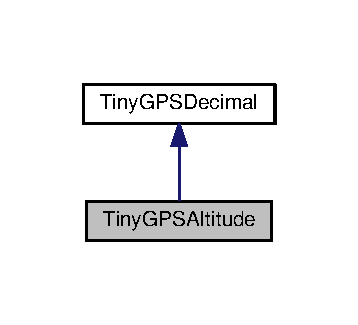
\includegraphics[width=172pt]{struct_tiny_g_p_s_altitude__inherit__graph}
\end{center}
\end{figure}


Collaboration diagram for Tiny\+G\+P\+S\+Altitude\+:\nopagebreak
\begin{figure}[H]
\begin{center}
\leavevmode
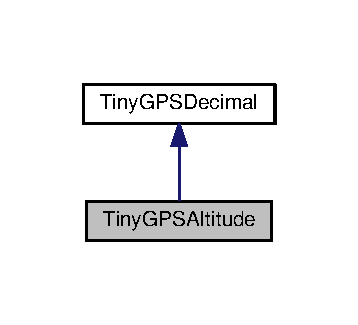
\includegraphics[width=172pt]{struct_tiny_g_p_s_altitude__coll__graph}
\end{center}
\end{figure}
\subsection*{Public Member Functions}
\begin{DoxyCompactItemize}
\item 
double \hyperlink{struct_tiny_g_p_s_altitude_a5a39d145bb1778814007206c765189f7}{meters} ()
\item 
double \hyperlink{struct_tiny_g_p_s_altitude_a5ae68d990ea08d4e21cfa6aefb46cc03}{miles} ()
\item 
double \hyperlink{struct_tiny_g_p_s_altitude_a1eb3e5b425784fc0db3e9ffe0f77f741}{kilometers} ()
\item 
double \hyperlink{struct_tiny_g_p_s_altitude_ac782babc0c485d47e6f57384e88b8cc8}{feet} ()
\end{DoxyCompactItemize}


\subsection{Detailed Description}


Definition at line 179 of file Tiny\+G\+P\+S++.\+h.



\subsection{Member Function Documentation}
\index{Tiny\+G\+P\+S\+Altitude@{Tiny\+G\+P\+S\+Altitude}!feet@{feet}}
\index{feet@{feet}!Tiny\+G\+P\+S\+Altitude@{Tiny\+G\+P\+S\+Altitude}}
\subsubsection[{\texorpdfstring{feet()}{feet()}}]{\setlength{\rightskip}{0pt plus 5cm}double Tiny\+G\+P\+S\+Altitude\+::feet (
\begin{DoxyParamCaption}
{}
\end{DoxyParamCaption}
)\hspace{0.3cm}{\ttfamily [inline]}}\hypertarget{struct_tiny_g_p_s_altitude_ac782babc0c485d47e6f57384e88b8cc8}{}\label{struct_tiny_g_p_s_altitude_ac782babc0c485d47e6f57384e88b8cc8}


Definition at line 184 of file Tiny\+G\+P\+S++.\+h.

\index{Tiny\+G\+P\+S\+Altitude@{Tiny\+G\+P\+S\+Altitude}!kilometers@{kilometers}}
\index{kilometers@{kilometers}!Tiny\+G\+P\+S\+Altitude@{Tiny\+G\+P\+S\+Altitude}}
\subsubsection[{\texorpdfstring{kilometers()}{kilometers()}}]{\setlength{\rightskip}{0pt plus 5cm}double Tiny\+G\+P\+S\+Altitude\+::kilometers (
\begin{DoxyParamCaption}
{}
\end{DoxyParamCaption}
)\hspace{0.3cm}{\ttfamily [inline]}}\hypertarget{struct_tiny_g_p_s_altitude_a1eb3e5b425784fc0db3e9ffe0f77f741}{}\label{struct_tiny_g_p_s_altitude_a1eb3e5b425784fc0db3e9ffe0f77f741}


Definition at line 183 of file Tiny\+G\+P\+S++.\+h.

\index{Tiny\+G\+P\+S\+Altitude@{Tiny\+G\+P\+S\+Altitude}!meters@{meters}}
\index{meters@{meters}!Tiny\+G\+P\+S\+Altitude@{Tiny\+G\+P\+S\+Altitude}}
\subsubsection[{\texorpdfstring{meters()}{meters()}}]{\setlength{\rightskip}{0pt plus 5cm}double Tiny\+G\+P\+S\+Altitude\+::meters (
\begin{DoxyParamCaption}
{}
\end{DoxyParamCaption}
)\hspace{0.3cm}{\ttfamily [inline]}}\hypertarget{struct_tiny_g_p_s_altitude_a5a39d145bb1778814007206c765189f7}{}\label{struct_tiny_g_p_s_altitude_a5a39d145bb1778814007206c765189f7}


Definition at line 181 of file Tiny\+G\+P\+S++.\+h.

\index{Tiny\+G\+P\+S\+Altitude@{Tiny\+G\+P\+S\+Altitude}!miles@{miles}}
\index{miles@{miles}!Tiny\+G\+P\+S\+Altitude@{Tiny\+G\+P\+S\+Altitude}}
\subsubsection[{\texorpdfstring{miles()}{miles()}}]{\setlength{\rightskip}{0pt plus 5cm}double Tiny\+G\+P\+S\+Altitude\+::miles (
\begin{DoxyParamCaption}
{}
\end{DoxyParamCaption}
)\hspace{0.3cm}{\ttfamily [inline]}}\hypertarget{struct_tiny_g_p_s_altitude_a5ae68d990ea08d4e21cfa6aefb46cc03}{}\label{struct_tiny_g_p_s_altitude_a5ae68d990ea08d4e21cfa6aefb46cc03}


Definition at line 182 of file Tiny\+G\+P\+S++.\+h.



The documentation for this struct was generated from the following file\+:\begin{DoxyCompactItemize}
\item 
lib/\+Tiny\+G\+P\+S\+Plus/\hyperlink{_tiny_g_p_s_09_09_8h}{Tiny\+G\+P\+S++.\+h}\end{DoxyCompactItemize}

\hypertarget{struct_tiny_g_p_s_course}{}\section{Tiny\+G\+P\+S\+Course Struct Reference}
\label{struct_tiny_g_p_s_course}\index{Tiny\+G\+P\+S\+Course@{Tiny\+G\+P\+S\+Course}}


{\ttfamily \#include $<$Tiny\+G\+P\+S++.\+h$>$}



Inheritance diagram for Tiny\+G\+P\+S\+Course\+:\nopagebreak
\begin{figure}[H]
\begin{center}
\leavevmode
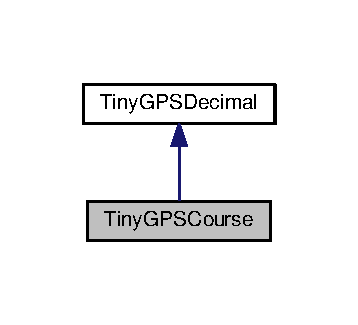
\includegraphics[width=172pt]{struct_tiny_g_p_s_course__inherit__graph}
\end{center}
\end{figure}


Collaboration diagram for Tiny\+G\+P\+S\+Course\+:\nopagebreak
\begin{figure}[H]
\begin{center}
\leavevmode
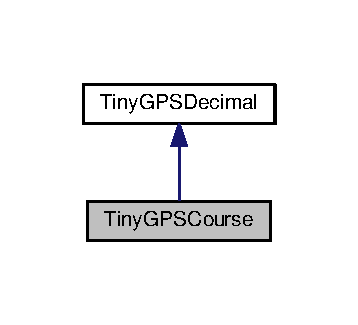
\includegraphics[width=172pt]{struct_tiny_g_p_s_course__coll__graph}
\end{center}
\end{figure}
\subsection*{Public Member Functions}
\begin{DoxyCompactItemize}
\item 
double \hyperlink{struct_tiny_g_p_s_course_a76dc8ae6c2fe5ead9b44c8d53a3272ca}{deg} ()
\end{DoxyCompactItemize}


\subsection{Detailed Description}


Definition at line 174 of file Tiny\+G\+P\+S++.\+h.



\subsection{Member Function Documentation}
\index{Tiny\+G\+P\+S\+Course@{Tiny\+G\+P\+S\+Course}!deg@{deg}}
\index{deg@{deg}!Tiny\+G\+P\+S\+Course@{Tiny\+G\+P\+S\+Course}}
\subsubsection[{\texorpdfstring{deg()}{deg()}}]{\setlength{\rightskip}{0pt plus 5cm}double Tiny\+G\+P\+S\+Course\+::deg (
\begin{DoxyParamCaption}
{}
\end{DoxyParamCaption}
)\hspace{0.3cm}{\ttfamily [inline]}}\hypertarget{struct_tiny_g_p_s_course_a76dc8ae6c2fe5ead9b44c8d53a3272ca}{}\label{struct_tiny_g_p_s_course_a76dc8ae6c2fe5ead9b44c8d53a3272ca}


Definition at line 176 of file Tiny\+G\+P\+S++.\+h.



The documentation for this struct was generated from the following file\+:\begin{DoxyCompactItemize}
\item 
lib/\+Tiny\+G\+P\+S\+Plus/\hyperlink{_tiny_g_p_s_09_09_8h}{Tiny\+G\+P\+S++.\+h}\end{DoxyCompactItemize}

\hypertarget{class_tiny_g_p_s_custom}{}\section{Tiny\+G\+P\+S\+Custom Class Reference}
\label{class_tiny_g_p_s_custom}\index{Tiny\+G\+P\+S\+Custom@{Tiny\+G\+P\+S\+Custom}}


{\ttfamily \#include $<$Tiny\+G\+P\+S++.\+h$>$}

\subsection*{Public Member Functions}
\begin{DoxyCompactItemize}
\item 
\hyperlink{class_tiny_g_p_s_custom_ac82fa99f3bcd9811377dd5fa3e9e98c7}{Tiny\+G\+P\+S\+Custom} ()
\item 
\hyperlink{class_tiny_g_p_s_custom_a29b2a658bf95d8e6265e983b1c0251b5}{Tiny\+G\+P\+S\+Custom} (\hyperlink{class_tiny_g_p_s_plus}{Tiny\+G\+P\+S\+Plus} \&gps, const char $\ast$sentence\+Name, int term\+Number)
\item 
void \hyperlink{class_tiny_g_p_s_custom_a3bf972f7e2e7e3f483071630e5ca8355}{begin} (\hyperlink{class_tiny_g_p_s_plus}{Tiny\+G\+P\+S\+Plus} \&gps, const char $\ast$\+\_\+sentence\+Name, int \+\_\+term\+Number)
\item 
bool \hyperlink{class_tiny_g_p_s_custom_a3905509b3f88d67e248855c135744b14}{is\+Updated} () const 
\item 
bool \hyperlink{class_tiny_g_p_s_custom_a06fad8448c014424bf96ed379b55da21}{is\+Valid} () const 
\item 
uint32\+\_\+t \hyperlink{class_tiny_g_p_s_custom_a9bacaf774b1dba9ad942435d3ed1c2cc}{age} () const 
\item 
const char $\ast$ \hyperlink{class_tiny_g_p_s_custom_ac5ad40a3d9b6fe386b2309f972566674}{value} ()
\end{DoxyCompactItemize}
\subsection*{Friends}
\begin{DoxyCompactItemize}
\item 
class \hyperlink{class_tiny_g_p_s_custom_a6501fd5ef19ae166d43e0e5781609ee2}{Tiny\+G\+P\+S\+Plus}
\end{DoxyCompactItemize}


\subsection{Detailed Description}


Definition at line 188 of file Tiny\+G\+P\+S++.\+h.



\subsection{Constructor \& Destructor Documentation}
\index{Tiny\+G\+P\+S\+Custom@{Tiny\+G\+P\+S\+Custom}!Tiny\+G\+P\+S\+Custom@{Tiny\+G\+P\+S\+Custom}}
\index{Tiny\+G\+P\+S\+Custom@{Tiny\+G\+P\+S\+Custom}!Tiny\+G\+P\+S\+Custom@{Tiny\+G\+P\+S\+Custom}}
\subsubsection[{\texorpdfstring{Tiny\+G\+P\+S\+Custom()}{TinyGPSCustom()}}]{\setlength{\rightskip}{0pt plus 5cm}Tiny\+G\+P\+S\+Custom\+::\+Tiny\+G\+P\+S\+Custom (
\begin{DoxyParamCaption}
{}
\end{DoxyParamCaption}
)\hspace{0.3cm}{\ttfamily [inline]}}\hypertarget{class_tiny_g_p_s_custom_ac82fa99f3bcd9811377dd5fa3e9e98c7}{}\label{class_tiny_g_p_s_custom_ac82fa99f3bcd9811377dd5fa3e9e98c7}


Definition at line 191 of file Tiny\+G\+P\+S++.\+h.

\index{Tiny\+G\+P\+S\+Custom@{Tiny\+G\+P\+S\+Custom}!Tiny\+G\+P\+S\+Custom@{Tiny\+G\+P\+S\+Custom}}
\index{Tiny\+G\+P\+S\+Custom@{Tiny\+G\+P\+S\+Custom}!Tiny\+G\+P\+S\+Custom@{Tiny\+G\+P\+S\+Custom}}
\subsubsection[{\texorpdfstring{Tiny\+G\+P\+S\+Custom(\+Tiny\+G\+P\+S\+Plus \&gps, const char $\ast$sentence\+Name, int term\+Number)}{TinyGPSCustom(TinyGPSPlus &gps, const char *sentenceName, int termNumber)}}]{\setlength{\rightskip}{0pt plus 5cm}Tiny\+G\+P\+S\+Custom\+::\+Tiny\+G\+P\+S\+Custom (
\begin{DoxyParamCaption}
\item[{{\bf Tiny\+G\+P\+S\+Plus} \&}]{gps, }
\item[{const char $\ast$}]{sentence\+Name, }
\item[{int}]{term\+Number}
\end{DoxyParamCaption}
)}\hypertarget{class_tiny_g_p_s_custom_a29b2a658bf95d8e6265e983b1c0251b5}{}\label{class_tiny_g_p_s_custom_a29b2a658bf95d8e6265e983b1c0251b5}


Definition at line 460 of file Tiny\+G\+P\+S++.\+cpp.



\subsection{Member Function Documentation}
\index{Tiny\+G\+P\+S\+Custom@{Tiny\+G\+P\+S\+Custom}!age@{age}}
\index{age@{age}!Tiny\+G\+P\+S\+Custom@{Tiny\+G\+P\+S\+Custom}}
\subsubsection[{\texorpdfstring{age() const }{age() const }}]{\setlength{\rightskip}{0pt plus 5cm}uint32\+\_\+t Tiny\+G\+P\+S\+Custom\+::age (
\begin{DoxyParamCaption}
{}
\end{DoxyParamCaption}
) const\hspace{0.3cm}{\ttfamily [inline]}}\hypertarget{class_tiny_g_p_s_custom_a9bacaf774b1dba9ad942435d3ed1c2cc}{}\label{class_tiny_g_p_s_custom_a9bacaf774b1dba9ad942435d3ed1c2cc}


Definition at line 197 of file Tiny\+G\+P\+S++.\+h.

\index{Tiny\+G\+P\+S\+Custom@{Tiny\+G\+P\+S\+Custom}!begin@{begin}}
\index{begin@{begin}!Tiny\+G\+P\+S\+Custom@{Tiny\+G\+P\+S\+Custom}}
\subsubsection[{\texorpdfstring{begin(\+Tiny\+G\+P\+S\+Plus \&gps, const char $\ast$\+\_\+sentence\+Name, int \+\_\+term\+Number)}{begin(TinyGPSPlus &gps, const char *_sentenceName, int _termNumber)}}]{\setlength{\rightskip}{0pt plus 5cm}void Tiny\+G\+P\+S\+Custom\+::begin (
\begin{DoxyParamCaption}
\item[{{\bf Tiny\+G\+P\+S\+Plus} \&}]{gps, }
\item[{const char $\ast$}]{\+\_\+sentence\+Name, }
\item[{int}]{\+\_\+term\+Number}
\end{DoxyParamCaption}
)}\hypertarget{class_tiny_g_p_s_custom_a3bf972f7e2e7e3f483071630e5ca8355}{}\label{class_tiny_g_p_s_custom_a3bf972f7e2e7e3f483071630e5ca8355}


Definition at line 465 of file Tiny\+G\+P\+S++.\+cpp.

\index{Tiny\+G\+P\+S\+Custom@{Tiny\+G\+P\+S\+Custom}!is\+Updated@{is\+Updated}}
\index{is\+Updated@{is\+Updated}!Tiny\+G\+P\+S\+Custom@{Tiny\+G\+P\+S\+Custom}}
\subsubsection[{\texorpdfstring{is\+Updated() const }{isUpdated() const }}]{\setlength{\rightskip}{0pt plus 5cm}bool Tiny\+G\+P\+S\+Custom\+::is\+Updated (
\begin{DoxyParamCaption}
{}
\end{DoxyParamCaption}
) const\hspace{0.3cm}{\ttfamily [inline]}}\hypertarget{class_tiny_g_p_s_custom_a3905509b3f88d67e248855c135744b14}{}\label{class_tiny_g_p_s_custom_a3905509b3f88d67e248855c135744b14}


Definition at line 195 of file Tiny\+G\+P\+S++.\+h.

\index{Tiny\+G\+P\+S\+Custom@{Tiny\+G\+P\+S\+Custom}!is\+Valid@{is\+Valid}}
\index{is\+Valid@{is\+Valid}!Tiny\+G\+P\+S\+Custom@{Tiny\+G\+P\+S\+Custom}}
\subsubsection[{\texorpdfstring{is\+Valid() const }{isValid() const }}]{\setlength{\rightskip}{0pt plus 5cm}bool Tiny\+G\+P\+S\+Custom\+::is\+Valid (
\begin{DoxyParamCaption}
{}
\end{DoxyParamCaption}
) const\hspace{0.3cm}{\ttfamily [inline]}}\hypertarget{class_tiny_g_p_s_custom_a06fad8448c014424bf96ed379b55da21}{}\label{class_tiny_g_p_s_custom_a06fad8448c014424bf96ed379b55da21}


Definition at line 196 of file Tiny\+G\+P\+S++.\+h.

\index{Tiny\+G\+P\+S\+Custom@{Tiny\+G\+P\+S\+Custom}!value@{value}}
\index{value@{value}!Tiny\+G\+P\+S\+Custom@{Tiny\+G\+P\+S\+Custom}}
\subsubsection[{\texorpdfstring{value()}{value()}}]{\setlength{\rightskip}{0pt plus 5cm}const char$\ast$ Tiny\+G\+P\+S\+Custom\+::value (
\begin{DoxyParamCaption}
{}
\end{DoxyParamCaption}
)\hspace{0.3cm}{\ttfamily [inline]}}\hypertarget{class_tiny_g_p_s_custom_ac5ad40a3d9b6fe386b2309f972566674}{}\label{class_tiny_g_p_s_custom_ac5ad40a3d9b6fe386b2309f972566674}


Definition at line 198 of file Tiny\+G\+P\+S++.\+h.



\subsection{Friends And Related Function Documentation}
\index{Tiny\+G\+P\+S\+Custom@{Tiny\+G\+P\+S\+Custom}!Tiny\+G\+P\+S\+Plus@{Tiny\+G\+P\+S\+Plus}}
\index{Tiny\+G\+P\+S\+Plus@{Tiny\+G\+P\+S\+Plus}!Tiny\+G\+P\+S\+Custom@{Tiny\+G\+P\+S\+Custom}}
\subsubsection[{\texorpdfstring{Tiny\+G\+P\+S\+Plus}{TinyGPSPlus}}]{\setlength{\rightskip}{0pt plus 5cm}friend class {\bf Tiny\+G\+P\+S\+Plus}\hspace{0.3cm}{\ttfamily [friend]}}\hypertarget{class_tiny_g_p_s_custom_a6501fd5ef19ae166d43e0e5781609ee2}{}\label{class_tiny_g_p_s_custom_a6501fd5ef19ae166d43e0e5781609ee2}


Definition at line 210 of file Tiny\+G\+P\+S++.\+h.



The documentation for this class was generated from the following files\+:\begin{DoxyCompactItemize}
\item 
lib/\+Tiny\+G\+P\+S\+Plus/\hyperlink{_tiny_g_p_s_09_09_8h}{Tiny\+G\+P\+S++.\+h}\item 
lib/\+Tiny\+G\+P\+S\+Plus/\hyperlink{_tiny_g_p_s_09_09_8cpp}{Tiny\+G\+P\+S++.\+cpp}\end{DoxyCompactItemize}

\hypertarget{struct_tiny_g_p_s_date}{}\section{Tiny\+G\+P\+S\+Date Struct Reference}
\label{struct_tiny_g_p_s_date}\index{Tiny\+G\+P\+S\+Date@{Tiny\+G\+P\+S\+Date}}


{\ttfamily \#include $<$Tiny\+G\+P\+S++.\+h$>$}

\subsection*{Public Member Functions}
\begin{DoxyCompactItemize}
\item 
bool \hyperlink{struct_tiny_g_p_s_date_a0ef145848ab03e4e9db0e2cf3a4c42cd}{is\+Valid} () const 
\item 
bool \hyperlink{struct_tiny_g_p_s_date_aed8706c1c3e67558fec2b94476c144e0}{is\+Updated} () const 
\item 
uint32\+\_\+t \hyperlink{struct_tiny_g_p_s_date_a7b92ac9058dbde1770eb52ce5da890c1}{age} () const 
\item 
uint32\+\_\+t \hyperlink{struct_tiny_g_p_s_date_a718150ae16f68afa9ae81f9d1b3ce3f4}{value} ()
\item 
uint16\+\_\+t \hyperlink{struct_tiny_g_p_s_date_ae2cc914fec377b429d99f01204f50d60}{year} ()
\item 
uint8\+\_\+t \hyperlink{struct_tiny_g_p_s_date_a6f3c5b4e72ef28b010f94ac9016315f3}{month} ()
\item 
uint8\+\_\+t \hyperlink{struct_tiny_g_p_s_date_ae8cc5f80c49e328f792d168a44062000}{day} ()
\item 
\hyperlink{struct_tiny_g_p_s_date_a4d5f23eb008cbfd385343687bf902003}{Tiny\+G\+P\+S\+Date} ()
\end{DoxyCompactItemize}
\subsection*{Friends}
\begin{DoxyCompactItemize}
\item 
class \hyperlink{struct_tiny_g_p_s_date_a6501fd5ef19ae166d43e0e5781609ee2}{Tiny\+G\+P\+S\+Plus}
\end{DoxyCompactItemize}


\subsection{Detailed Description}


Definition at line 77 of file Tiny\+G\+P\+S++.\+h.



\subsection{Constructor \& Destructor Documentation}
\index{Tiny\+G\+P\+S\+Date@{Tiny\+G\+P\+S\+Date}!Tiny\+G\+P\+S\+Date@{Tiny\+G\+P\+S\+Date}}
\index{Tiny\+G\+P\+S\+Date@{Tiny\+G\+P\+S\+Date}!Tiny\+G\+P\+S\+Date@{Tiny\+G\+P\+S\+Date}}
\subsubsection[{\texorpdfstring{Tiny\+G\+P\+S\+Date()}{TinyGPSDate()}}]{\setlength{\rightskip}{0pt plus 5cm}Tiny\+G\+P\+S\+Date\+::\+Tiny\+G\+P\+S\+Date (
\begin{DoxyParamCaption}
{}
\end{DoxyParamCaption}
)\hspace{0.3cm}{\ttfamily [inline]}}\hypertarget{struct_tiny_g_p_s_date_a4d5f23eb008cbfd385343687bf902003}{}\label{struct_tiny_g_p_s_date_a4d5f23eb008cbfd385343687bf902003}


Definition at line 90 of file Tiny\+G\+P\+S++.\+h.



\subsection{Member Function Documentation}
\index{Tiny\+G\+P\+S\+Date@{Tiny\+G\+P\+S\+Date}!age@{age}}
\index{age@{age}!Tiny\+G\+P\+S\+Date@{Tiny\+G\+P\+S\+Date}}
\subsubsection[{\texorpdfstring{age() const }{age() const }}]{\setlength{\rightskip}{0pt plus 5cm}uint32\+\_\+t Tiny\+G\+P\+S\+Date\+::age (
\begin{DoxyParamCaption}
{}
\end{DoxyParamCaption}
) const\hspace{0.3cm}{\ttfamily [inline]}}\hypertarget{struct_tiny_g_p_s_date_a7b92ac9058dbde1770eb52ce5da890c1}{}\label{struct_tiny_g_p_s_date_a7b92ac9058dbde1770eb52ce5da890c1}


Definition at line 83 of file Tiny\+G\+P\+S++.\+h.

\index{Tiny\+G\+P\+S\+Date@{Tiny\+G\+P\+S\+Date}!day@{day}}
\index{day@{day}!Tiny\+G\+P\+S\+Date@{Tiny\+G\+P\+S\+Date}}
\subsubsection[{\texorpdfstring{day()}{day()}}]{\setlength{\rightskip}{0pt plus 5cm}uint8\+\_\+t Tiny\+G\+P\+S\+Date\+::day (
\begin{DoxyParamCaption}
{}
\end{DoxyParamCaption}
)}\hypertarget{struct_tiny_g_p_s_date_ae8cc5f80c49e328f792d168a44062000}{}\label{struct_tiny_g_p_s_date_ae8cc5f80c49e328f792d168a44062000}


Definition at line 406 of file Tiny\+G\+P\+S++.\+cpp.

\index{Tiny\+G\+P\+S\+Date@{Tiny\+G\+P\+S\+Date}!is\+Updated@{is\+Updated}}
\index{is\+Updated@{is\+Updated}!Tiny\+G\+P\+S\+Date@{Tiny\+G\+P\+S\+Date}}
\subsubsection[{\texorpdfstring{is\+Updated() const }{isUpdated() const }}]{\setlength{\rightskip}{0pt plus 5cm}bool Tiny\+G\+P\+S\+Date\+::is\+Updated (
\begin{DoxyParamCaption}
{}
\end{DoxyParamCaption}
) const\hspace{0.3cm}{\ttfamily [inline]}}\hypertarget{struct_tiny_g_p_s_date_aed8706c1c3e67558fec2b94476c144e0}{}\label{struct_tiny_g_p_s_date_aed8706c1c3e67558fec2b94476c144e0}


Definition at line 82 of file Tiny\+G\+P\+S++.\+h.

\index{Tiny\+G\+P\+S\+Date@{Tiny\+G\+P\+S\+Date}!is\+Valid@{is\+Valid}}
\index{is\+Valid@{is\+Valid}!Tiny\+G\+P\+S\+Date@{Tiny\+G\+P\+S\+Date}}
\subsubsection[{\texorpdfstring{is\+Valid() const }{isValid() const }}]{\setlength{\rightskip}{0pt plus 5cm}bool Tiny\+G\+P\+S\+Date\+::is\+Valid (
\begin{DoxyParamCaption}
{}
\end{DoxyParamCaption}
) const\hspace{0.3cm}{\ttfamily [inline]}}\hypertarget{struct_tiny_g_p_s_date_a0ef145848ab03e4e9db0e2cf3a4c42cd}{}\label{struct_tiny_g_p_s_date_a0ef145848ab03e4e9db0e2cf3a4c42cd}


Definition at line 81 of file Tiny\+G\+P\+S++.\+h.

\index{Tiny\+G\+P\+S\+Date@{Tiny\+G\+P\+S\+Date}!month@{month}}
\index{month@{month}!Tiny\+G\+P\+S\+Date@{Tiny\+G\+P\+S\+Date}}
\subsubsection[{\texorpdfstring{month()}{month()}}]{\setlength{\rightskip}{0pt plus 5cm}uint8\+\_\+t Tiny\+G\+P\+S\+Date\+::month (
\begin{DoxyParamCaption}
{}
\end{DoxyParamCaption}
)}\hypertarget{struct_tiny_g_p_s_date_a6f3c5b4e72ef28b010f94ac9016315f3}{}\label{struct_tiny_g_p_s_date_a6f3c5b4e72ef28b010f94ac9016315f3}


Definition at line 400 of file Tiny\+G\+P\+S++.\+cpp.

\index{Tiny\+G\+P\+S\+Date@{Tiny\+G\+P\+S\+Date}!value@{value}}
\index{value@{value}!Tiny\+G\+P\+S\+Date@{Tiny\+G\+P\+S\+Date}}
\subsubsection[{\texorpdfstring{value()}{value()}}]{\setlength{\rightskip}{0pt plus 5cm}uint32\+\_\+t Tiny\+G\+P\+S\+Date\+::value (
\begin{DoxyParamCaption}
{}
\end{DoxyParamCaption}
)\hspace{0.3cm}{\ttfamily [inline]}}\hypertarget{struct_tiny_g_p_s_date_a718150ae16f68afa9ae81f9d1b3ce3f4}{}\label{struct_tiny_g_p_s_date_a718150ae16f68afa9ae81f9d1b3ce3f4}


Definition at line 85 of file Tiny\+G\+P\+S++.\+h.

\index{Tiny\+G\+P\+S\+Date@{Tiny\+G\+P\+S\+Date}!year@{year}}
\index{year@{year}!Tiny\+G\+P\+S\+Date@{Tiny\+G\+P\+S\+Date}}
\subsubsection[{\texorpdfstring{year()}{year()}}]{\setlength{\rightskip}{0pt plus 5cm}uint16\+\_\+t Tiny\+G\+P\+S\+Date\+::year (
\begin{DoxyParamCaption}
{}
\end{DoxyParamCaption}
)}\hypertarget{struct_tiny_g_p_s_date_ae2cc914fec377b429d99f01204f50d60}{}\label{struct_tiny_g_p_s_date_ae2cc914fec377b429d99f01204f50d60}


Definition at line 393 of file Tiny\+G\+P\+S++.\+cpp.



\subsection{Friends And Related Function Documentation}
\index{Tiny\+G\+P\+S\+Date@{Tiny\+G\+P\+S\+Date}!Tiny\+G\+P\+S\+Plus@{Tiny\+G\+P\+S\+Plus}}
\index{Tiny\+G\+P\+S\+Plus@{Tiny\+G\+P\+S\+Plus}!Tiny\+G\+P\+S\+Date@{Tiny\+G\+P\+S\+Date}}
\subsubsection[{\texorpdfstring{Tiny\+G\+P\+S\+Plus}{TinyGPSPlus}}]{\setlength{\rightskip}{0pt plus 5cm}friend class {\bf Tiny\+G\+P\+S\+Plus}\hspace{0.3cm}{\ttfamily [friend]}}\hypertarget{struct_tiny_g_p_s_date_a6501fd5ef19ae166d43e0e5781609ee2}{}\label{struct_tiny_g_p_s_date_a6501fd5ef19ae166d43e0e5781609ee2}


Definition at line 79 of file Tiny\+G\+P\+S++.\+h.



The documentation for this struct was generated from the following files\+:\begin{DoxyCompactItemize}
\item 
lib/\+Tiny\+G\+P\+S\+Plus/\hyperlink{_tiny_g_p_s_09_09_8h}{Tiny\+G\+P\+S++.\+h}\item 
lib/\+Tiny\+G\+P\+S\+Plus/\hyperlink{_tiny_g_p_s_09_09_8cpp}{Tiny\+G\+P\+S++.\+cpp}\end{DoxyCompactItemize}

\hypertarget{struct_tiny_g_p_s_decimal}{}\section{Tiny\+G\+P\+S\+Decimal Struct Reference}
\label{struct_tiny_g_p_s_decimal}\index{Tiny\+G\+P\+S\+Decimal@{Tiny\+G\+P\+S\+Decimal}}


{\ttfamily \#include $<$Tiny\+G\+P\+S++.\+h$>$}



Inheritance diagram for Tiny\+G\+P\+S\+Decimal\+:\nopagebreak
\begin{figure}[H]
\begin{center}
\leavevmode
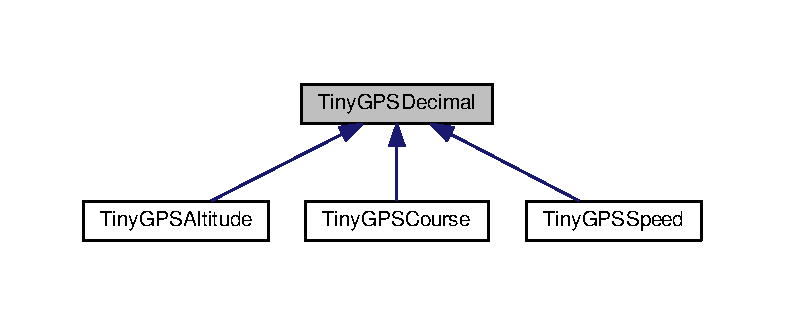
\includegraphics[width=350pt]{struct_tiny_g_p_s_decimal__inherit__graph}
\end{center}
\end{figure}
\subsection*{Public Member Functions}
\begin{DoxyCompactItemize}
\item 
bool \hyperlink{struct_tiny_g_p_s_decimal_a2a1d868525e903eb193b7a36cdd76984}{is\+Valid} () const 
\item 
bool \hyperlink{struct_tiny_g_p_s_decimal_ae8b7f9f7719c2974ebd3b34759493d15}{is\+Updated} () const 
\item 
uint32\+\_\+t \hyperlink{struct_tiny_g_p_s_decimal_ab80191a3e02c92ad3f674b5df2ab752f}{age} () const 
\item 
int32\+\_\+t \hyperlink{struct_tiny_g_p_s_decimal_ac3ce80976e5d8456e9f211b910a6cb19}{value} ()
\item 
\hyperlink{struct_tiny_g_p_s_decimal_ae09cbb1856cd57c7dcee52fb5fb1ba16}{Tiny\+G\+P\+S\+Decimal} ()
\end{DoxyCompactItemize}
\subsection*{Friends}
\begin{DoxyCompactItemize}
\item 
class \hyperlink{struct_tiny_g_p_s_decimal_a6501fd5ef19ae166d43e0e5781609ee2}{Tiny\+G\+P\+S\+Plus}
\end{DoxyCompactItemize}


\subsection{Detailed Description}


Definition at line 126 of file Tiny\+G\+P\+S++.\+h.



\subsection{Constructor \& Destructor Documentation}
\index{Tiny\+G\+P\+S\+Decimal@{Tiny\+G\+P\+S\+Decimal}!Tiny\+G\+P\+S\+Decimal@{Tiny\+G\+P\+S\+Decimal}}
\index{Tiny\+G\+P\+S\+Decimal@{Tiny\+G\+P\+S\+Decimal}!Tiny\+G\+P\+S\+Decimal@{Tiny\+G\+P\+S\+Decimal}}
\subsubsection[{\texorpdfstring{Tiny\+G\+P\+S\+Decimal()}{TinyGPSDecimal()}}]{\setlength{\rightskip}{0pt plus 5cm}Tiny\+G\+P\+S\+Decimal\+::\+Tiny\+G\+P\+S\+Decimal (
\begin{DoxyParamCaption}
{}
\end{DoxyParamCaption}
)\hspace{0.3cm}{\ttfamily [inline]}}\hypertarget{struct_tiny_g_p_s_decimal_ae09cbb1856cd57c7dcee52fb5fb1ba16}{}\label{struct_tiny_g_p_s_decimal_ae09cbb1856cd57c7dcee52fb5fb1ba16}


Definition at line 135 of file Tiny\+G\+P\+S++.\+h.



\subsection{Member Function Documentation}
\index{Tiny\+G\+P\+S\+Decimal@{Tiny\+G\+P\+S\+Decimal}!age@{age}}
\index{age@{age}!Tiny\+G\+P\+S\+Decimal@{Tiny\+G\+P\+S\+Decimal}}
\subsubsection[{\texorpdfstring{age() const }{age() const }}]{\setlength{\rightskip}{0pt plus 5cm}uint32\+\_\+t Tiny\+G\+P\+S\+Decimal\+::age (
\begin{DoxyParamCaption}
{}
\end{DoxyParamCaption}
) const\hspace{0.3cm}{\ttfamily [inline]}}\hypertarget{struct_tiny_g_p_s_decimal_ab80191a3e02c92ad3f674b5df2ab752f}{}\label{struct_tiny_g_p_s_decimal_ab80191a3e02c92ad3f674b5df2ab752f}


Definition at line 132 of file Tiny\+G\+P\+S++.\+h.

\index{Tiny\+G\+P\+S\+Decimal@{Tiny\+G\+P\+S\+Decimal}!is\+Updated@{is\+Updated}}
\index{is\+Updated@{is\+Updated}!Tiny\+G\+P\+S\+Decimal@{Tiny\+G\+P\+S\+Decimal}}
\subsubsection[{\texorpdfstring{is\+Updated() const }{isUpdated() const }}]{\setlength{\rightskip}{0pt plus 5cm}bool Tiny\+G\+P\+S\+Decimal\+::is\+Updated (
\begin{DoxyParamCaption}
{}
\end{DoxyParamCaption}
) const\hspace{0.3cm}{\ttfamily [inline]}}\hypertarget{struct_tiny_g_p_s_decimal_ae8b7f9f7719c2974ebd3b34759493d15}{}\label{struct_tiny_g_p_s_decimal_ae8b7f9f7719c2974ebd3b34759493d15}


Definition at line 131 of file Tiny\+G\+P\+S++.\+h.

\index{Tiny\+G\+P\+S\+Decimal@{Tiny\+G\+P\+S\+Decimal}!is\+Valid@{is\+Valid}}
\index{is\+Valid@{is\+Valid}!Tiny\+G\+P\+S\+Decimal@{Tiny\+G\+P\+S\+Decimal}}
\subsubsection[{\texorpdfstring{is\+Valid() const }{isValid() const }}]{\setlength{\rightskip}{0pt plus 5cm}bool Tiny\+G\+P\+S\+Decimal\+::is\+Valid (
\begin{DoxyParamCaption}
{}
\end{DoxyParamCaption}
) const\hspace{0.3cm}{\ttfamily [inline]}}\hypertarget{struct_tiny_g_p_s_decimal_a2a1d868525e903eb193b7a36cdd76984}{}\label{struct_tiny_g_p_s_decimal_a2a1d868525e903eb193b7a36cdd76984}


Definition at line 130 of file Tiny\+G\+P\+S++.\+h.

\index{Tiny\+G\+P\+S\+Decimal@{Tiny\+G\+P\+S\+Decimal}!value@{value}}
\index{value@{value}!Tiny\+G\+P\+S\+Decimal@{Tiny\+G\+P\+S\+Decimal}}
\subsubsection[{\texorpdfstring{value()}{value()}}]{\setlength{\rightskip}{0pt plus 5cm}int32\+\_\+t Tiny\+G\+P\+S\+Decimal\+::value (
\begin{DoxyParamCaption}
{}
\end{DoxyParamCaption}
)\hspace{0.3cm}{\ttfamily [inline]}}\hypertarget{struct_tiny_g_p_s_decimal_ac3ce80976e5d8456e9f211b910a6cb19}{}\label{struct_tiny_g_p_s_decimal_ac3ce80976e5d8456e9f211b910a6cb19}


Definition at line 133 of file Tiny\+G\+P\+S++.\+h.



\subsection{Friends And Related Function Documentation}
\index{Tiny\+G\+P\+S\+Decimal@{Tiny\+G\+P\+S\+Decimal}!Tiny\+G\+P\+S\+Plus@{Tiny\+G\+P\+S\+Plus}}
\index{Tiny\+G\+P\+S\+Plus@{Tiny\+G\+P\+S\+Plus}!Tiny\+G\+P\+S\+Decimal@{Tiny\+G\+P\+S\+Decimal}}
\subsubsection[{\texorpdfstring{Tiny\+G\+P\+S\+Plus}{TinyGPSPlus}}]{\setlength{\rightskip}{0pt plus 5cm}friend class {\bf Tiny\+G\+P\+S\+Plus}\hspace{0.3cm}{\ttfamily [friend]}}\hypertarget{struct_tiny_g_p_s_decimal_a6501fd5ef19ae166d43e0e5781609ee2}{}\label{struct_tiny_g_p_s_decimal_a6501fd5ef19ae166d43e0e5781609ee2}


Definition at line 128 of file Tiny\+G\+P\+S++.\+h.



The documentation for this struct was generated from the following files\+:\begin{DoxyCompactItemize}
\item 
lib/\+Tiny\+G\+P\+S\+Plus/\hyperlink{_tiny_g_p_s_09_09_8h}{Tiny\+G\+P\+S++.\+h}\item 
lib/\+Tiny\+G\+P\+S\+Plus/\hyperlink{_tiny_g_p_s_09_09_8cpp}{Tiny\+G\+P\+S++.\+cpp}\end{DoxyCompactItemize}

\hypertarget{struct_tiny_g_p_s_integer}{}\section{Tiny\+G\+P\+S\+Integer Struct Reference}
\label{struct_tiny_g_p_s_integer}\index{Tiny\+G\+P\+S\+Integer@{Tiny\+G\+P\+S\+Integer}}


{\ttfamily \#include $<$Tiny\+G\+P\+S++.\+h$>$}

\subsection*{Public Member Functions}
\begin{DoxyCompactItemize}
\item 
bool \hyperlink{struct_tiny_g_p_s_integer_aad411b5eb6cc16774ff0ff8d275df2fa}{is\+Valid} () const 
\item 
bool \hyperlink{struct_tiny_g_p_s_integer_aa6479670272df580287f84938183dc20}{is\+Updated} () const 
\item 
uint32\+\_\+t \hyperlink{struct_tiny_g_p_s_integer_a46ea8f4fe8cca279b7d4cd44572e5881}{age} () const 
\item 
uint32\+\_\+t \hyperlink{struct_tiny_g_p_s_integer_a67de7e76d61dbd25eb32f701d8ce867b}{value} ()
\item 
\hyperlink{struct_tiny_g_p_s_integer_a017a71970fa652964a9e71b7ec945cec}{Tiny\+G\+P\+S\+Integer} ()
\end{DoxyCompactItemize}
\subsection*{Friends}
\begin{DoxyCompactItemize}
\item 
class \hyperlink{struct_tiny_g_p_s_integer_a6501fd5ef19ae166d43e0e5781609ee2}{Tiny\+G\+P\+S\+Plus}
\end{DoxyCompactItemize}


\subsection{Detailed Description}


Definition at line 146 of file Tiny\+G\+P\+S++.\+h.



\subsection{Constructor \& Destructor Documentation}
\index{Tiny\+G\+P\+S\+Integer@{Tiny\+G\+P\+S\+Integer}!Tiny\+G\+P\+S\+Integer@{Tiny\+G\+P\+S\+Integer}}
\index{Tiny\+G\+P\+S\+Integer@{Tiny\+G\+P\+S\+Integer}!Tiny\+G\+P\+S\+Integer@{Tiny\+G\+P\+S\+Integer}}
\subsubsection[{\texorpdfstring{Tiny\+G\+P\+S\+Integer()}{TinyGPSInteger()}}]{\setlength{\rightskip}{0pt plus 5cm}Tiny\+G\+P\+S\+Integer\+::\+Tiny\+G\+P\+S\+Integer (
\begin{DoxyParamCaption}
{}
\end{DoxyParamCaption}
)\hspace{0.3cm}{\ttfamily [inline]}}\hypertarget{struct_tiny_g_p_s_integer_a017a71970fa652964a9e71b7ec945cec}{}\label{struct_tiny_g_p_s_integer_a017a71970fa652964a9e71b7ec945cec}


Definition at line 155 of file Tiny\+G\+P\+S++.\+h.



\subsection{Member Function Documentation}
\index{Tiny\+G\+P\+S\+Integer@{Tiny\+G\+P\+S\+Integer}!age@{age}}
\index{age@{age}!Tiny\+G\+P\+S\+Integer@{Tiny\+G\+P\+S\+Integer}}
\subsubsection[{\texorpdfstring{age() const }{age() const }}]{\setlength{\rightskip}{0pt plus 5cm}uint32\+\_\+t Tiny\+G\+P\+S\+Integer\+::age (
\begin{DoxyParamCaption}
{}
\end{DoxyParamCaption}
) const\hspace{0.3cm}{\ttfamily [inline]}}\hypertarget{struct_tiny_g_p_s_integer_a46ea8f4fe8cca279b7d4cd44572e5881}{}\label{struct_tiny_g_p_s_integer_a46ea8f4fe8cca279b7d4cd44572e5881}


Definition at line 152 of file Tiny\+G\+P\+S++.\+h.

\index{Tiny\+G\+P\+S\+Integer@{Tiny\+G\+P\+S\+Integer}!is\+Updated@{is\+Updated}}
\index{is\+Updated@{is\+Updated}!Tiny\+G\+P\+S\+Integer@{Tiny\+G\+P\+S\+Integer}}
\subsubsection[{\texorpdfstring{is\+Updated() const }{isUpdated() const }}]{\setlength{\rightskip}{0pt plus 5cm}bool Tiny\+G\+P\+S\+Integer\+::is\+Updated (
\begin{DoxyParamCaption}
{}
\end{DoxyParamCaption}
) const\hspace{0.3cm}{\ttfamily [inline]}}\hypertarget{struct_tiny_g_p_s_integer_aa6479670272df580287f84938183dc20}{}\label{struct_tiny_g_p_s_integer_aa6479670272df580287f84938183dc20}


Definition at line 151 of file Tiny\+G\+P\+S++.\+h.

\index{Tiny\+G\+P\+S\+Integer@{Tiny\+G\+P\+S\+Integer}!is\+Valid@{is\+Valid}}
\index{is\+Valid@{is\+Valid}!Tiny\+G\+P\+S\+Integer@{Tiny\+G\+P\+S\+Integer}}
\subsubsection[{\texorpdfstring{is\+Valid() const }{isValid() const }}]{\setlength{\rightskip}{0pt plus 5cm}bool Tiny\+G\+P\+S\+Integer\+::is\+Valid (
\begin{DoxyParamCaption}
{}
\end{DoxyParamCaption}
) const\hspace{0.3cm}{\ttfamily [inline]}}\hypertarget{struct_tiny_g_p_s_integer_aad411b5eb6cc16774ff0ff8d275df2fa}{}\label{struct_tiny_g_p_s_integer_aad411b5eb6cc16774ff0ff8d275df2fa}


Definition at line 150 of file Tiny\+G\+P\+S++.\+h.

\index{Tiny\+G\+P\+S\+Integer@{Tiny\+G\+P\+S\+Integer}!value@{value}}
\index{value@{value}!Tiny\+G\+P\+S\+Integer@{Tiny\+G\+P\+S\+Integer}}
\subsubsection[{\texorpdfstring{value()}{value()}}]{\setlength{\rightskip}{0pt plus 5cm}uint32\+\_\+t Tiny\+G\+P\+S\+Integer\+::value (
\begin{DoxyParamCaption}
{}
\end{DoxyParamCaption}
)\hspace{0.3cm}{\ttfamily [inline]}}\hypertarget{struct_tiny_g_p_s_integer_a67de7e76d61dbd25eb32f701d8ce867b}{}\label{struct_tiny_g_p_s_integer_a67de7e76d61dbd25eb32f701d8ce867b}


Definition at line 153 of file Tiny\+G\+P\+S++.\+h.



\subsection{Friends And Related Function Documentation}
\index{Tiny\+G\+P\+S\+Integer@{Tiny\+G\+P\+S\+Integer}!Tiny\+G\+P\+S\+Plus@{Tiny\+G\+P\+S\+Plus}}
\index{Tiny\+G\+P\+S\+Plus@{Tiny\+G\+P\+S\+Plus}!Tiny\+G\+P\+S\+Integer@{Tiny\+G\+P\+S\+Integer}}
\subsubsection[{\texorpdfstring{Tiny\+G\+P\+S\+Plus}{TinyGPSPlus}}]{\setlength{\rightskip}{0pt plus 5cm}friend class {\bf Tiny\+G\+P\+S\+Plus}\hspace{0.3cm}{\ttfamily [friend]}}\hypertarget{struct_tiny_g_p_s_integer_a6501fd5ef19ae166d43e0e5781609ee2}{}\label{struct_tiny_g_p_s_integer_a6501fd5ef19ae166d43e0e5781609ee2}


Definition at line 148 of file Tiny\+G\+P\+S++.\+h.



The documentation for this struct was generated from the following files\+:\begin{DoxyCompactItemize}
\item 
lib/\+Tiny\+G\+P\+S\+Plus/\hyperlink{_tiny_g_p_s_09_09_8h}{Tiny\+G\+P\+S++.\+h}\item 
lib/\+Tiny\+G\+P\+S\+Plus/\hyperlink{_tiny_g_p_s_09_09_8cpp}{Tiny\+G\+P\+S++.\+cpp}\end{DoxyCompactItemize}

\hypertarget{struct_tiny_g_p_s_location}{}\section{Tiny\+G\+P\+S\+Location Struct Reference}
\label{struct_tiny_g_p_s_location}\index{Tiny\+G\+P\+S\+Location@{Tiny\+G\+P\+S\+Location}}


{\ttfamily \#include $<$Tiny\+G\+P\+S++.\+h$>$}

\subsection*{Public Member Functions}
\begin{DoxyCompactItemize}
\item 
bool \hyperlink{struct_tiny_g_p_s_location_a783c2898915440f51a6df233aba51923}{is\+Valid} () const 
\item 
bool \hyperlink{struct_tiny_g_p_s_location_a9aae0a5fd73c2dab231309f1dd3b2c0a}{is\+Updated} () const 
\item 
uint32\+\_\+t \hyperlink{struct_tiny_g_p_s_location_ada111e1b74f82dc029c0c61241424ca8}{age} () const 
\item 
const \hyperlink{struct_raw_degrees}{Raw\+Degrees} \& \hyperlink{struct_tiny_g_p_s_location_abe2a4fbfe28299aae87c5b4c3c58bcad}{raw\+Lat} ()
\item 
const \hyperlink{struct_raw_degrees}{Raw\+Degrees} \& \hyperlink{struct_tiny_g_p_s_location_a9fe126feca0bdcfa9224a428b86d68db}{raw\+Lng} ()
\item 
double \hyperlink{struct_tiny_g_p_s_location_a86c3acea4f317b427eebb667e4d05a49}{lat} ()
\item 
double \hyperlink{struct_tiny_g_p_s_location_a544e9009a5580b2fd5466821a5e5b782}{lng} ()
\item 
\hyperlink{struct_tiny_g_p_s_location_a9bc435af16c3c5224fcd4b5c40d0c70f}{Tiny\+G\+P\+S\+Location} ()
\end{DoxyCompactItemize}
\subsection*{Friends}
\begin{DoxyCompactItemize}
\item 
class \hyperlink{struct_tiny_g_p_s_location_a6501fd5ef19ae166d43e0e5781609ee2}{Tiny\+G\+P\+S\+Plus}
\end{DoxyCompactItemize}


\subsection{Detailed Description}


Definition at line 53 of file Tiny\+G\+P\+S++.\+h.



\subsection{Constructor \& Destructor Documentation}
\index{Tiny\+G\+P\+S\+Location@{Tiny\+G\+P\+S\+Location}!Tiny\+G\+P\+S\+Location@{Tiny\+G\+P\+S\+Location}}
\index{Tiny\+G\+P\+S\+Location@{Tiny\+G\+P\+S\+Location}!Tiny\+G\+P\+S\+Location@{Tiny\+G\+P\+S\+Location}}
\subsubsection[{\texorpdfstring{Tiny\+G\+P\+S\+Location()}{TinyGPSLocation()}}]{\setlength{\rightskip}{0pt plus 5cm}Tiny\+G\+P\+S\+Location\+::\+Tiny\+G\+P\+S\+Location (
\begin{DoxyParamCaption}
{}
\end{DoxyParamCaption}
)\hspace{0.3cm}{\ttfamily [inline]}}\hypertarget{struct_tiny_g_p_s_location_a9bc435af16c3c5224fcd4b5c40d0c70f}{}\label{struct_tiny_g_p_s_location_a9bc435af16c3c5224fcd4b5c40d0c70f}


Definition at line 65 of file Tiny\+G\+P\+S++.\+h.



\subsection{Member Function Documentation}
\index{Tiny\+G\+P\+S\+Location@{Tiny\+G\+P\+S\+Location}!age@{age}}
\index{age@{age}!Tiny\+G\+P\+S\+Location@{Tiny\+G\+P\+S\+Location}}
\subsubsection[{\texorpdfstring{age() const }{age() const }}]{\setlength{\rightskip}{0pt plus 5cm}uint32\+\_\+t Tiny\+G\+P\+S\+Location\+::age (
\begin{DoxyParamCaption}
{}
\end{DoxyParamCaption}
) const\hspace{0.3cm}{\ttfamily [inline]}}\hypertarget{struct_tiny_g_p_s_location_ada111e1b74f82dc029c0c61241424ca8}{}\label{struct_tiny_g_p_s_location_ada111e1b74f82dc029c0c61241424ca8}


Definition at line 59 of file Tiny\+G\+P\+S++.\+h.

\index{Tiny\+G\+P\+S\+Location@{Tiny\+G\+P\+S\+Location}!is\+Updated@{is\+Updated}}
\index{is\+Updated@{is\+Updated}!Tiny\+G\+P\+S\+Location@{Tiny\+G\+P\+S\+Location}}
\subsubsection[{\texorpdfstring{is\+Updated() const }{isUpdated() const }}]{\setlength{\rightskip}{0pt plus 5cm}bool Tiny\+G\+P\+S\+Location\+::is\+Updated (
\begin{DoxyParamCaption}
{}
\end{DoxyParamCaption}
) const\hspace{0.3cm}{\ttfamily [inline]}}\hypertarget{struct_tiny_g_p_s_location_a9aae0a5fd73c2dab231309f1dd3b2c0a}{}\label{struct_tiny_g_p_s_location_a9aae0a5fd73c2dab231309f1dd3b2c0a}


Definition at line 58 of file Tiny\+G\+P\+S++.\+h.

\index{Tiny\+G\+P\+S\+Location@{Tiny\+G\+P\+S\+Location}!is\+Valid@{is\+Valid}}
\index{is\+Valid@{is\+Valid}!Tiny\+G\+P\+S\+Location@{Tiny\+G\+P\+S\+Location}}
\subsubsection[{\texorpdfstring{is\+Valid() const }{isValid() const }}]{\setlength{\rightskip}{0pt plus 5cm}bool Tiny\+G\+P\+S\+Location\+::is\+Valid (
\begin{DoxyParamCaption}
{}
\end{DoxyParamCaption}
) const\hspace{0.3cm}{\ttfamily [inline]}}\hypertarget{struct_tiny_g_p_s_location_a783c2898915440f51a6df233aba51923}{}\label{struct_tiny_g_p_s_location_a783c2898915440f51a6df233aba51923}


Definition at line 57 of file Tiny\+G\+P\+S++.\+h.

\index{Tiny\+G\+P\+S\+Location@{Tiny\+G\+P\+S\+Location}!lat@{lat}}
\index{lat@{lat}!Tiny\+G\+P\+S\+Location@{Tiny\+G\+P\+S\+Location}}
\subsubsection[{\texorpdfstring{lat()}{lat()}}]{\setlength{\rightskip}{0pt plus 5cm}double Tiny\+G\+P\+S\+Location\+::lat (
\begin{DoxyParamCaption}
{}
\end{DoxyParamCaption}
)}\hypertarget{struct_tiny_g_p_s_location_a86c3acea4f317b427eebb667e4d05a49}{}\label{struct_tiny_g_p_s_location_a86c3acea4f317b427eebb667e4d05a49}


Definition at line 355 of file Tiny\+G\+P\+S++.\+cpp.

\index{Tiny\+G\+P\+S\+Location@{Tiny\+G\+P\+S\+Location}!lng@{lng}}
\index{lng@{lng}!Tiny\+G\+P\+S\+Location@{Tiny\+G\+P\+S\+Location}}
\subsubsection[{\texorpdfstring{lng()}{lng()}}]{\setlength{\rightskip}{0pt plus 5cm}double Tiny\+G\+P\+S\+Location\+::lng (
\begin{DoxyParamCaption}
{}
\end{DoxyParamCaption}
)}\hypertarget{struct_tiny_g_p_s_location_a544e9009a5580b2fd5466821a5e5b782}{}\label{struct_tiny_g_p_s_location_a544e9009a5580b2fd5466821a5e5b782}


Definition at line 362 of file Tiny\+G\+P\+S++.\+cpp.

\index{Tiny\+G\+P\+S\+Location@{Tiny\+G\+P\+S\+Location}!raw\+Lat@{raw\+Lat}}
\index{raw\+Lat@{raw\+Lat}!Tiny\+G\+P\+S\+Location@{Tiny\+G\+P\+S\+Location}}
\subsubsection[{\texorpdfstring{raw\+Lat()}{rawLat()}}]{\setlength{\rightskip}{0pt plus 5cm}const {\bf Raw\+Degrees}\& Tiny\+G\+P\+S\+Location\+::raw\+Lat (
\begin{DoxyParamCaption}
{}
\end{DoxyParamCaption}
)\hspace{0.3cm}{\ttfamily [inline]}}\hypertarget{struct_tiny_g_p_s_location_abe2a4fbfe28299aae87c5b4c3c58bcad}{}\label{struct_tiny_g_p_s_location_abe2a4fbfe28299aae87c5b4c3c58bcad}


Definition at line 60 of file Tiny\+G\+P\+S++.\+h.

\index{Tiny\+G\+P\+S\+Location@{Tiny\+G\+P\+S\+Location}!raw\+Lng@{raw\+Lng}}
\index{raw\+Lng@{raw\+Lng}!Tiny\+G\+P\+S\+Location@{Tiny\+G\+P\+S\+Location}}
\subsubsection[{\texorpdfstring{raw\+Lng()}{rawLng()}}]{\setlength{\rightskip}{0pt plus 5cm}const {\bf Raw\+Degrees}\& Tiny\+G\+P\+S\+Location\+::raw\+Lng (
\begin{DoxyParamCaption}
{}
\end{DoxyParamCaption}
)\hspace{0.3cm}{\ttfamily [inline]}}\hypertarget{struct_tiny_g_p_s_location_a9fe126feca0bdcfa9224a428b86d68db}{}\label{struct_tiny_g_p_s_location_a9fe126feca0bdcfa9224a428b86d68db}


Definition at line 61 of file Tiny\+G\+P\+S++.\+h.



\subsection{Friends And Related Function Documentation}
\index{Tiny\+G\+P\+S\+Location@{Tiny\+G\+P\+S\+Location}!Tiny\+G\+P\+S\+Plus@{Tiny\+G\+P\+S\+Plus}}
\index{Tiny\+G\+P\+S\+Plus@{Tiny\+G\+P\+S\+Plus}!Tiny\+G\+P\+S\+Location@{Tiny\+G\+P\+S\+Location}}
\subsubsection[{\texorpdfstring{Tiny\+G\+P\+S\+Plus}{TinyGPSPlus}}]{\setlength{\rightskip}{0pt plus 5cm}friend class {\bf Tiny\+G\+P\+S\+Plus}\hspace{0.3cm}{\ttfamily [friend]}}\hypertarget{struct_tiny_g_p_s_location_a6501fd5ef19ae166d43e0e5781609ee2}{}\label{struct_tiny_g_p_s_location_a6501fd5ef19ae166d43e0e5781609ee2}


Definition at line 55 of file Tiny\+G\+P\+S++.\+h.



The documentation for this struct was generated from the following files\+:\begin{DoxyCompactItemize}
\item 
lib/\+Tiny\+G\+P\+S\+Plus/\hyperlink{_tiny_g_p_s_09_09_8h}{Tiny\+G\+P\+S++.\+h}\item 
lib/\+Tiny\+G\+P\+S\+Plus/\hyperlink{_tiny_g_p_s_09_09_8cpp}{Tiny\+G\+P\+S++.\+cpp}\end{DoxyCompactItemize}

\hypertarget{class_tiny_g_p_s_plus}{}\section{Tiny\+G\+P\+S\+Plus Class Reference}
\label{class_tiny_g_p_s_plus}\index{Tiny\+G\+P\+S\+Plus@{Tiny\+G\+P\+S\+Plus}}


{\ttfamily \#include $<$Tiny\+G\+P\+S++.\+h$>$}



Collaboration diagram for Tiny\+G\+P\+S\+Plus\+:\nopagebreak
\begin{figure}[H]
\begin{center}
\leavevmode
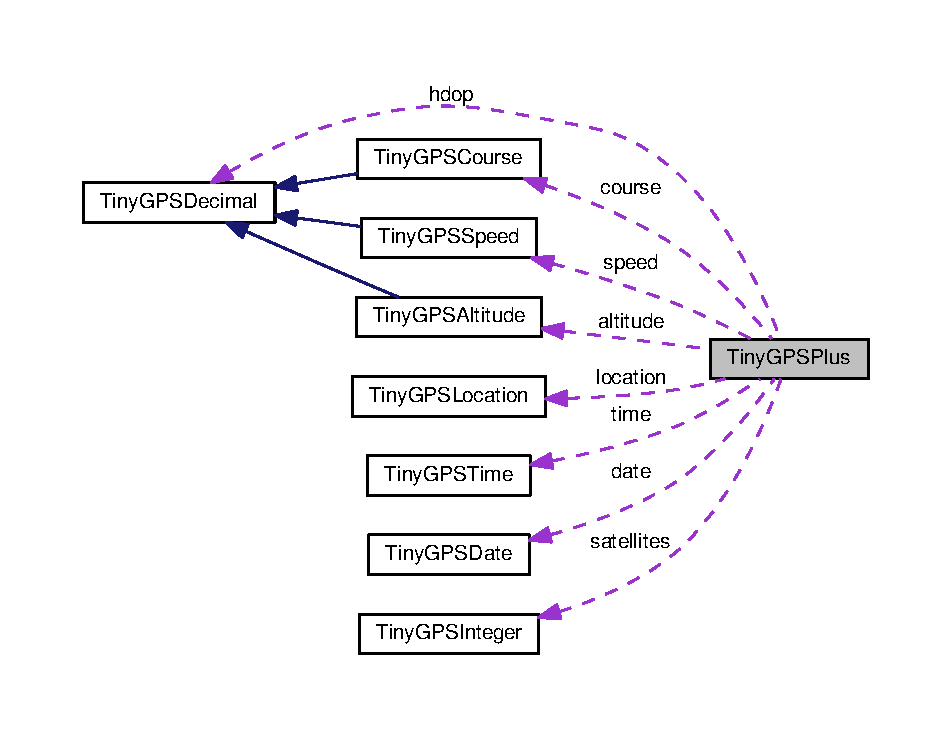
\includegraphics[width=350pt]{class_tiny_g_p_s_plus__coll__graph}
\end{center}
\end{figure}
\subsection*{Public Member Functions}
\begin{DoxyCompactItemize}
\item 
\hyperlink{class_tiny_g_p_s_plus_a3d9173312d514abf50bd43efe6bf6af3}{Tiny\+G\+P\+S\+Plus} ()
\item 
bool \hyperlink{class_tiny_g_p_s_plus_ad7b78320b7e4967df17c6a27008a5154}{encode} (char c)
\item 
\hyperlink{class_tiny_g_p_s_plus}{Tiny\+G\+P\+S\+Plus} \& \hyperlink{class_tiny_g_p_s_plus_a32a0b61a25ce0c490216cb2b4ea19ced}{operator$<$$<$} (char c)
\item 
uint32\+\_\+t \hyperlink{class_tiny_g_p_s_plus_a12b6bc0169ee6b2f0beb8041e549f338}{chars\+Processed} () const 
\item 
uint32\+\_\+t \hyperlink{class_tiny_g_p_s_plus_a6c502ec591dc42a83771a502c4dbdcd4}{sentences\+With\+Fix} () const 
\item 
uint32\+\_\+t \hyperlink{class_tiny_g_p_s_plus_a57dd7a4430d58f784e967ee2d76e574f}{failed\+Checksum} () const 
\item 
uint32\+\_\+t \hyperlink{class_tiny_g_p_s_plus_a55af5d3442bf8f5c5fdd0309e416d9e5}{passed\+Checksum} () const 
\end{DoxyCompactItemize}
\subsection*{Static Public Member Functions}
\begin{DoxyCompactItemize}
\item 
static const char $\ast$ \hyperlink{class_tiny_g_p_s_plus_a1ec39648e1c80c59f4fded642fdb88ae}{library\+Version} ()
\item 
static double \hyperlink{class_tiny_g_p_s_plus_ace607cf3a6d49628e44eae1232237138}{distance\+Between} (double lat1, double long1, double lat2, double long2)
\item 
static double \hyperlink{class_tiny_g_p_s_plus_af338c18ccf58a47659be1ffc8259541d}{course\+To} (double lat1, double long1, double lat2, double long2)
\item 
static const char $\ast$ \hyperlink{class_tiny_g_p_s_plus_a8c9e9444552ff85a505ffc6933dda03c}{cardinal} (double \hyperlink{class_tiny_g_p_s_plus_ad7800d3decbe58e355f5229bba231868}{course})
\item 
static int32\+\_\+t \hyperlink{class_tiny_g_p_s_plus_a06d9bf0c1f0d0963511dc05e2f121121}{parse\+Decimal} (const char $\ast$term)
\item 
static void \hyperlink{class_tiny_g_p_s_plus_a00627eaffc625bf366e4c984014fbf29}{parse\+Degrees} (const char $\ast$term, \hyperlink{struct_raw_degrees}{Raw\+Degrees} \&deg)
\end{DoxyCompactItemize}
\subsection*{Public Attributes}
\begin{DoxyCompactItemize}
\item 
\hyperlink{struct_tiny_g_p_s_location}{Tiny\+G\+P\+S\+Location} \hyperlink{class_tiny_g_p_s_plus_a886255f412f8e01f84e5104d36315fb3}{location}
\item 
\hyperlink{struct_tiny_g_p_s_date}{Tiny\+G\+P\+S\+Date} \hyperlink{class_tiny_g_p_s_plus_a83a70812b432d7f51c7c735bfe7be0f0}{date}
\item 
\hyperlink{struct_tiny_g_p_s_time}{Tiny\+G\+P\+S\+Time} \hyperlink{class_tiny_g_p_s_plus_a377c975527fa24b45fb86356505eb134}{time}
\item 
\hyperlink{struct_tiny_g_p_s_speed}{Tiny\+G\+P\+S\+Speed} \hyperlink{class_tiny_g_p_s_plus_aa085c3e72a399a829dd92af52b373404}{speed}
\item 
\hyperlink{struct_tiny_g_p_s_course}{Tiny\+G\+P\+S\+Course} \hyperlink{class_tiny_g_p_s_plus_ad7800d3decbe58e355f5229bba231868}{course}
\item 
\hyperlink{struct_tiny_g_p_s_altitude}{Tiny\+G\+P\+S\+Altitude} \hyperlink{class_tiny_g_p_s_plus_a0b3451a4ee75e5880ffd88c3038eacf8}{altitude}
\item 
\hyperlink{struct_tiny_g_p_s_integer}{Tiny\+G\+P\+S\+Integer} \hyperlink{class_tiny_g_p_s_plus_a5fb47066d1d03f4bb5853529053aab48}{satellites}
\item 
\hyperlink{struct_tiny_g_p_s_decimal}{Tiny\+G\+P\+S\+Decimal} \hyperlink{class_tiny_g_p_s_plus_a3a21b3ae7085bb278b35d703bf135632}{hdop}
\end{DoxyCompactItemize}
\subsection*{Friends}
\begin{DoxyCompactItemize}
\item 
class \hyperlink{class_tiny_g_p_s_plus_aaad5bf5a2728a81e624ad2304f817772}{Tiny\+G\+P\+S\+Custom}
\end{DoxyCompactItemize}


\subsection{Detailed Description}


Definition at line 214 of file Tiny\+G\+P\+S++.\+h.



\subsection{Constructor \& Destructor Documentation}
\index{Tiny\+G\+P\+S\+Plus@{Tiny\+G\+P\+S\+Plus}!Tiny\+G\+P\+S\+Plus@{Tiny\+G\+P\+S\+Plus}}
\index{Tiny\+G\+P\+S\+Plus@{Tiny\+G\+P\+S\+Plus}!Tiny\+G\+P\+S\+Plus@{Tiny\+G\+P\+S\+Plus}}
\subsubsection[{\texorpdfstring{Tiny\+G\+P\+S\+Plus()}{TinyGPSPlus()}}]{\setlength{\rightskip}{0pt plus 5cm}Tiny\+G\+P\+S\+Plus\+::\+Tiny\+G\+P\+S\+Plus (
\begin{DoxyParamCaption}
{}
\end{DoxyParamCaption}
)}\hypertarget{class_tiny_g_p_s_plus_a3d9173312d514abf50bd43efe6bf6af3}{}\label{class_tiny_g_p_s_plus_a3d9173312d514abf50bd43efe6bf6af3}


Definition at line 35 of file Tiny\+G\+P\+S++.\+cpp.



\subsection{Member Function Documentation}
\index{Tiny\+G\+P\+S\+Plus@{Tiny\+G\+P\+S\+Plus}!cardinal@{cardinal}}
\index{cardinal@{cardinal}!Tiny\+G\+P\+S\+Plus@{Tiny\+G\+P\+S\+Plus}}
\subsubsection[{\texorpdfstring{cardinal(double course)}{cardinal(double course)}}]{\setlength{\rightskip}{0pt plus 5cm}const char $\ast$ Tiny\+G\+P\+S\+Plus\+::cardinal (
\begin{DoxyParamCaption}
\item[{double}]{course}
\end{DoxyParamCaption}
)\hspace{0.3cm}{\ttfamily [static]}}\hypertarget{class_tiny_g_p_s_plus_a8c9e9444552ff85a505ffc6933dda03c}{}\label{class_tiny_g_p_s_plus_a8c9e9444552ff85a505ffc6933dda03c}


Definition at line 330 of file Tiny\+G\+P\+S++.\+cpp.

\index{Tiny\+G\+P\+S\+Plus@{Tiny\+G\+P\+S\+Plus}!chars\+Processed@{chars\+Processed}}
\index{chars\+Processed@{chars\+Processed}!Tiny\+G\+P\+S\+Plus@{Tiny\+G\+P\+S\+Plus}}
\subsubsection[{\texorpdfstring{chars\+Processed() const }{charsProcessed() const }}]{\setlength{\rightskip}{0pt plus 5cm}uint32\+\_\+t Tiny\+G\+P\+S\+Plus\+::chars\+Processed (
\begin{DoxyParamCaption}
{}
\end{DoxyParamCaption}
) const\hspace{0.3cm}{\ttfamily [inline]}}\hypertarget{class_tiny_g_p_s_plus_a12b6bc0169ee6b2f0beb8041e549f338}{}\label{class_tiny_g_p_s_plus_a12b6bc0169ee6b2f0beb8041e549f338}


Definition at line 239 of file Tiny\+G\+P\+S++.\+h.

\index{Tiny\+G\+P\+S\+Plus@{Tiny\+G\+P\+S\+Plus}!course\+To@{course\+To}}
\index{course\+To@{course\+To}!Tiny\+G\+P\+S\+Plus@{Tiny\+G\+P\+S\+Plus}}
\subsubsection[{\texorpdfstring{course\+To(double lat1, double long1, double lat2, double long2)}{courseTo(double lat1, double long1, double lat2, double long2)}}]{\setlength{\rightskip}{0pt plus 5cm}double Tiny\+G\+P\+S\+Plus\+::course\+To (
\begin{DoxyParamCaption}
\item[{double}]{lat1, }
\item[{double}]{long1, }
\item[{double}]{lat2, }
\item[{double}]{long2}
\end{DoxyParamCaption}
)\hspace{0.3cm}{\ttfamily [static]}}\hypertarget{class_tiny_g_p_s_plus_af338c18ccf58a47659be1ffc8259541d}{}\label{class_tiny_g_p_s_plus_af338c18ccf58a47659be1ffc8259541d}


Definition at line 310 of file Tiny\+G\+P\+S++.\+cpp.

\index{Tiny\+G\+P\+S\+Plus@{Tiny\+G\+P\+S\+Plus}!distance\+Between@{distance\+Between}}
\index{distance\+Between@{distance\+Between}!Tiny\+G\+P\+S\+Plus@{Tiny\+G\+P\+S\+Plus}}
\subsubsection[{\texorpdfstring{distance\+Between(double lat1, double long1, double lat2, double long2)}{distanceBetween(double lat1, double long1, double lat2, double long2)}}]{\setlength{\rightskip}{0pt plus 5cm}double Tiny\+G\+P\+S\+Plus\+::distance\+Between (
\begin{DoxyParamCaption}
\item[{double}]{lat1, }
\item[{double}]{long1, }
\item[{double}]{lat2, }
\item[{double}]{long2}
\end{DoxyParamCaption}
)\hspace{0.3cm}{\ttfamily [static]}}\hypertarget{class_tiny_g_p_s_plus_ace607cf3a6d49628e44eae1232237138}{}\label{class_tiny_g_p_s_plus_ace607cf3a6d49628e44eae1232237138}


Definition at line 285 of file Tiny\+G\+P\+S++.\+cpp.

\index{Tiny\+G\+P\+S\+Plus@{Tiny\+G\+P\+S\+Plus}!encode@{encode}}
\index{encode@{encode}!Tiny\+G\+P\+S\+Plus@{Tiny\+G\+P\+S\+Plus}}
\subsubsection[{\texorpdfstring{encode(char c)}{encode(char c)}}]{\setlength{\rightskip}{0pt plus 5cm}bool Tiny\+G\+P\+S\+Plus\+::encode (
\begin{DoxyParamCaption}
\item[{char}]{c}
\end{DoxyParamCaption}
)}\hypertarget{class_tiny_g_p_s_plus_ad7b78320b7e4967df17c6a27008a5154}{}\label{class_tiny_g_p_s_plus_ad7b78320b7e4967df17c6a27008a5154}


Definition at line 56 of file Tiny\+G\+P\+S++.\+cpp.

\index{Tiny\+G\+P\+S\+Plus@{Tiny\+G\+P\+S\+Plus}!failed\+Checksum@{failed\+Checksum}}
\index{failed\+Checksum@{failed\+Checksum}!Tiny\+G\+P\+S\+Plus@{Tiny\+G\+P\+S\+Plus}}
\subsubsection[{\texorpdfstring{failed\+Checksum() const }{failedChecksum() const }}]{\setlength{\rightskip}{0pt plus 5cm}uint32\+\_\+t Tiny\+G\+P\+S\+Plus\+::failed\+Checksum (
\begin{DoxyParamCaption}
{}
\end{DoxyParamCaption}
) const\hspace{0.3cm}{\ttfamily [inline]}}\hypertarget{class_tiny_g_p_s_plus_a57dd7a4430d58f784e967ee2d76e574f}{}\label{class_tiny_g_p_s_plus_a57dd7a4430d58f784e967ee2d76e574f}


Definition at line 241 of file Tiny\+G\+P\+S++.\+h.

\index{Tiny\+G\+P\+S\+Plus@{Tiny\+G\+P\+S\+Plus}!library\+Version@{library\+Version}}
\index{library\+Version@{library\+Version}!Tiny\+G\+P\+S\+Plus@{Tiny\+G\+P\+S\+Plus}}
\subsubsection[{\texorpdfstring{library\+Version()}{libraryVersion()}}]{\setlength{\rightskip}{0pt plus 5cm}static const char$\ast$ Tiny\+G\+P\+S\+Plus\+::library\+Version (
\begin{DoxyParamCaption}
{}
\end{DoxyParamCaption}
)\hspace{0.3cm}{\ttfamily [inline]}, {\ttfamily [static]}}\hypertarget{class_tiny_g_p_s_plus_a1ec39648e1c80c59f4fded642fdb88ae}{}\label{class_tiny_g_p_s_plus_a1ec39648e1c80c59f4fded642fdb88ae}


Definition at line 230 of file Tiny\+G\+P\+S++.\+h.

\index{Tiny\+G\+P\+S\+Plus@{Tiny\+G\+P\+S\+Plus}!operator$<$$<$@{operator$<$$<$}}
\index{operator$<$$<$@{operator$<$$<$}!Tiny\+G\+P\+S\+Plus@{Tiny\+G\+P\+S\+Plus}}
\subsubsection[{\texorpdfstring{operator$<$$<$(char c)}{operator<<(char c)}}]{\setlength{\rightskip}{0pt plus 5cm}{\bf Tiny\+G\+P\+S\+Plus}\& Tiny\+G\+P\+S\+Plus\+::operator$<$$<$ (
\begin{DoxyParamCaption}
\item[{char}]{c}
\end{DoxyParamCaption}
)\hspace{0.3cm}{\ttfamily [inline]}}\hypertarget{class_tiny_g_p_s_plus_a32a0b61a25ce0c490216cb2b4ea19ced}{}\label{class_tiny_g_p_s_plus_a32a0b61a25ce0c490216cb2b4ea19ced}


Definition at line 219 of file Tiny\+G\+P\+S++.\+h.

\index{Tiny\+G\+P\+S\+Plus@{Tiny\+G\+P\+S\+Plus}!parse\+Decimal@{parse\+Decimal}}
\index{parse\+Decimal@{parse\+Decimal}!Tiny\+G\+P\+S\+Plus@{Tiny\+G\+P\+S\+Plus}}
\subsubsection[{\texorpdfstring{parse\+Decimal(const char $\ast$term)}{parseDecimal(const char *term)}}]{\setlength{\rightskip}{0pt plus 5cm}int32\+\_\+t Tiny\+G\+P\+S\+Plus\+::parse\+Decimal (
\begin{DoxyParamCaption}
\item[{const char $\ast$}]{term}
\end{DoxyParamCaption}
)\hspace{0.3cm}{\ttfamily [static]}}\hypertarget{class_tiny_g_p_s_plus_a06d9bf0c1f0d0963511dc05e2f121121}{}\label{class_tiny_g_p_s_plus_a06d9bf0c1f0d0963511dc05e2f121121}


Definition at line 115 of file Tiny\+G\+P\+S++.\+cpp.

\index{Tiny\+G\+P\+S\+Plus@{Tiny\+G\+P\+S\+Plus}!parse\+Degrees@{parse\+Degrees}}
\index{parse\+Degrees@{parse\+Degrees}!Tiny\+G\+P\+S\+Plus@{Tiny\+G\+P\+S\+Plus}}
\subsubsection[{\texorpdfstring{parse\+Degrees(const char $\ast$term, Raw\+Degrees \&deg)}{parseDegrees(const char *term, RawDegrees &deg)}}]{\setlength{\rightskip}{0pt plus 5cm}void Tiny\+G\+P\+S\+Plus\+::parse\+Degrees (
\begin{DoxyParamCaption}
\item[{const char $\ast$}]{term, }
\item[{{\bf Raw\+Degrees} \&}]{deg}
\end{DoxyParamCaption}
)\hspace{0.3cm}{\ttfamily [static]}}\hypertarget{class_tiny_g_p_s_plus_a00627eaffc625bf366e4c984014fbf29}{}\label{class_tiny_g_p_s_plus_a00627eaffc625bf366e4c984014fbf29}


Definition at line 132 of file Tiny\+G\+P\+S++.\+cpp.

\index{Tiny\+G\+P\+S\+Plus@{Tiny\+G\+P\+S\+Plus}!passed\+Checksum@{passed\+Checksum}}
\index{passed\+Checksum@{passed\+Checksum}!Tiny\+G\+P\+S\+Plus@{Tiny\+G\+P\+S\+Plus}}
\subsubsection[{\texorpdfstring{passed\+Checksum() const }{passedChecksum() const }}]{\setlength{\rightskip}{0pt plus 5cm}uint32\+\_\+t Tiny\+G\+P\+S\+Plus\+::passed\+Checksum (
\begin{DoxyParamCaption}
{}
\end{DoxyParamCaption}
) const\hspace{0.3cm}{\ttfamily [inline]}}\hypertarget{class_tiny_g_p_s_plus_a55af5d3442bf8f5c5fdd0309e416d9e5}{}\label{class_tiny_g_p_s_plus_a55af5d3442bf8f5c5fdd0309e416d9e5}


Definition at line 242 of file Tiny\+G\+P\+S++.\+h.

\index{Tiny\+G\+P\+S\+Plus@{Tiny\+G\+P\+S\+Plus}!sentences\+With\+Fix@{sentences\+With\+Fix}}
\index{sentences\+With\+Fix@{sentences\+With\+Fix}!Tiny\+G\+P\+S\+Plus@{Tiny\+G\+P\+S\+Plus}}
\subsubsection[{\texorpdfstring{sentences\+With\+Fix() const }{sentencesWithFix() const }}]{\setlength{\rightskip}{0pt plus 5cm}uint32\+\_\+t Tiny\+G\+P\+S\+Plus\+::sentences\+With\+Fix (
\begin{DoxyParamCaption}
{}
\end{DoxyParamCaption}
) const\hspace{0.3cm}{\ttfamily [inline]}}\hypertarget{class_tiny_g_p_s_plus_a6c502ec591dc42a83771a502c4dbdcd4}{}\label{class_tiny_g_p_s_plus_a6c502ec591dc42a83771a502c4dbdcd4}


Definition at line 240 of file Tiny\+G\+P\+S++.\+h.



\subsection{Friends And Related Function Documentation}
\index{Tiny\+G\+P\+S\+Plus@{Tiny\+G\+P\+S\+Plus}!Tiny\+G\+P\+S\+Custom@{Tiny\+G\+P\+S\+Custom}}
\index{Tiny\+G\+P\+S\+Custom@{Tiny\+G\+P\+S\+Custom}!Tiny\+G\+P\+S\+Plus@{Tiny\+G\+P\+S\+Plus}}
\subsubsection[{\texorpdfstring{Tiny\+G\+P\+S\+Custom}{TinyGPSCustom}}]{\setlength{\rightskip}{0pt plus 5cm}friend class {\bf Tiny\+G\+P\+S\+Custom}\hspace{0.3cm}{\ttfamily [friend]}}\hypertarget{class_tiny_g_p_s_plus_aaad5bf5a2728a81e624ad2304f817772}{}\label{class_tiny_g_p_s_plus_aaad5bf5a2728a81e624ad2304f817772}


Definition at line 257 of file Tiny\+G\+P\+S++.\+h.



\subsection{Member Data Documentation}
\index{Tiny\+G\+P\+S\+Plus@{Tiny\+G\+P\+S\+Plus}!altitude@{altitude}}
\index{altitude@{altitude}!Tiny\+G\+P\+S\+Plus@{Tiny\+G\+P\+S\+Plus}}
\subsubsection[{\texorpdfstring{altitude}{altitude}}]{\setlength{\rightskip}{0pt plus 5cm}{\bf Tiny\+G\+P\+S\+Altitude} Tiny\+G\+P\+S\+Plus\+::altitude}\hypertarget{class_tiny_g_p_s_plus_a0b3451a4ee75e5880ffd88c3038eacf8}{}\label{class_tiny_g_p_s_plus_a0b3451a4ee75e5880ffd88c3038eacf8}


Definition at line 226 of file Tiny\+G\+P\+S++.\+h.

\index{Tiny\+G\+P\+S\+Plus@{Tiny\+G\+P\+S\+Plus}!course@{course}}
\index{course@{course}!Tiny\+G\+P\+S\+Plus@{Tiny\+G\+P\+S\+Plus}}
\subsubsection[{\texorpdfstring{course}{course}}]{\setlength{\rightskip}{0pt plus 5cm}{\bf Tiny\+G\+P\+S\+Course} Tiny\+G\+P\+S\+Plus\+::course}\hypertarget{class_tiny_g_p_s_plus_ad7800d3decbe58e355f5229bba231868}{}\label{class_tiny_g_p_s_plus_ad7800d3decbe58e355f5229bba231868}


Definition at line 225 of file Tiny\+G\+P\+S++.\+h.

\index{Tiny\+G\+P\+S\+Plus@{Tiny\+G\+P\+S\+Plus}!date@{date}}
\index{date@{date}!Tiny\+G\+P\+S\+Plus@{Tiny\+G\+P\+S\+Plus}}
\subsubsection[{\texorpdfstring{date}{date}}]{\setlength{\rightskip}{0pt plus 5cm}{\bf Tiny\+G\+P\+S\+Date} Tiny\+G\+P\+S\+Plus\+::date}\hypertarget{class_tiny_g_p_s_plus_a83a70812b432d7f51c7c735bfe7be0f0}{}\label{class_tiny_g_p_s_plus_a83a70812b432d7f51c7c735bfe7be0f0}


Definition at line 222 of file Tiny\+G\+P\+S++.\+h.

\index{Tiny\+G\+P\+S\+Plus@{Tiny\+G\+P\+S\+Plus}!hdop@{hdop}}
\index{hdop@{hdop}!Tiny\+G\+P\+S\+Plus@{Tiny\+G\+P\+S\+Plus}}
\subsubsection[{\texorpdfstring{hdop}{hdop}}]{\setlength{\rightskip}{0pt plus 5cm}{\bf Tiny\+G\+P\+S\+Decimal} Tiny\+G\+P\+S\+Plus\+::hdop}\hypertarget{class_tiny_g_p_s_plus_a3a21b3ae7085bb278b35d703bf135632}{}\label{class_tiny_g_p_s_plus_a3a21b3ae7085bb278b35d703bf135632}


Definition at line 228 of file Tiny\+G\+P\+S++.\+h.

\index{Tiny\+G\+P\+S\+Plus@{Tiny\+G\+P\+S\+Plus}!location@{location}}
\index{location@{location}!Tiny\+G\+P\+S\+Plus@{Tiny\+G\+P\+S\+Plus}}
\subsubsection[{\texorpdfstring{location}{location}}]{\setlength{\rightskip}{0pt plus 5cm}{\bf Tiny\+G\+P\+S\+Location} Tiny\+G\+P\+S\+Plus\+::location}\hypertarget{class_tiny_g_p_s_plus_a886255f412f8e01f84e5104d36315fb3}{}\label{class_tiny_g_p_s_plus_a886255f412f8e01f84e5104d36315fb3}


Definition at line 221 of file Tiny\+G\+P\+S++.\+h.

\index{Tiny\+G\+P\+S\+Plus@{Tiny\+G\+P\+S\+Plus}!satellites@{satellites}}
\index{satellites@{satellites}!Tiny\+G\+P\+S\+Plus@{Tiny\+G\+P\+S\+Plus}}
\subsubsection[{\texorpdfstring{satellites}{satellites}}]{\setlength{\rightskip}{0pt plus 5cm}{\bf Tiny\+G\+P\+S\+Integer} Tiny\+G\+P\+S\+Plus\+::satellites}\hypertarget{class_tiny_g_p_s_plus_a5fb47066d1d03f4bb5853529053aab48}{}\label{class_tiny_g_p_s_plus_a5fb47066d1d03f4bb5853529053aab48}


Definition at line 227 of file Tiny\+G\+P\+S++.\+h.

\index{Tiny\+G\+P\+S\+Plus@{Tiny\+G\+P\+S\+Plus}!speed@{speed}}
\index{speed@{speed}!Tiny\+G\+P\+S\+Plus@{Tiny\+G\+P\+S\+Plus}}
\subsubsection[{\texorpdfstring{speed}{speed}}]{\setlength{\rightskip}{0pt plus 5cm}{\bf Tiny\+G\+P\+S\+Speed} Tiny\+G\+P\+S\+Plus\+::speed}\hypertarget{class_tiny_g_p_s_plus_aa085c3e72a399a829dd92af52b373404}{}\label{class_tiny_g_p_s_plus_aa085c3e72a399a829dd92af52b373404}


Definition at line 224 of file Tiny\+G\+P\+S++.\+h.

\index{Tiny\+G\+P\+S\+Plus@{Tiny\+G\+P\+S\+Plus}!time@{time}}
\index{time@{time}!Tiny\+G\+P\+S\+Plus@{Tiny\+G\+P\+S\+Plus}}
\subsubsection[{\texorpdfstring{time}{time}}]{\setlength{\rightskip}{0pt plus 5cm}{\bf Tiny\+G\+P\+S\+Time} Tiny\+G\+P\+S\+Plus\+::time}\hypertarget{class_tiny_g_p_s_plus_a377c975527fa24b45fb86356505eb134}{}\label{class_tiny_g_p_s_plus_a377c975527fa24b45fb86356505eb134}


Definition at line 223 of file Tiny\+G\+P\+S++.\+h.



The documentation for this class was generated from the following files\+:\begin{DoxyCompactItemize}
\item 
lib/\+Tiny\+G\+P\+S\+Plus/\hyperlink{_tiny_g_p_s_09_09_8h}{Tiny\+G\+P\+S++.\+h}\item 
lib/\+Tiny\+G\+P\+S\+Plus/\hyperlink{_tiny_g_p_s_09_09_8cpp}{Tiny\+G\+P\+S++.\+cpp}\end{DoxyCompactItemize}

\hypertarget{struct_tiny_g_p_s_speed}{}\section{Tiny\+G\+P\+S\+Speed Struct Reference}
\label{struct_tiny_g_p_s_speed}\index{Tiny\+G\+P\+S\+Speed@{Tiny\+G\+P\+S\+Speed}}


{\ttfamily \#include $<$Tiny\+G\+P\+S++.\+h$>$}



Inheritance diagram for Tiny\+G\+P\+S\+Speed\+:\nopagebreak
\begin{figure}[H]
\begin{center}
\leavevmode
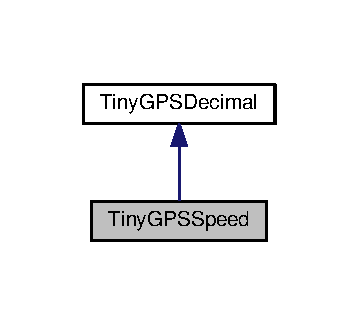
\includegraphics[width=172pt]{struct_tiny_g_p_s_speed__inherit__graph}
\end{center}
\end{figure}


Collaboration diagram for Tiny\+G\+P\+S\+Speed\+:\nopagebreak
\begin{figure}[H]
\begin{center}
\leavevmode
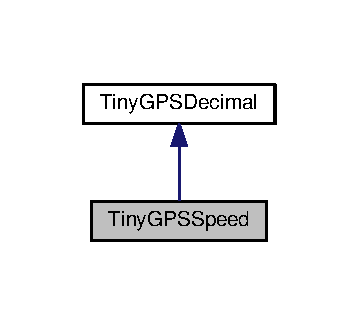
\includegraphics[width=172pt]{struct_tiny_g_p_s_speed__coll__graph}
\end{center}
\end{figure}
\subsection*{Public Member Functions}
\begin{DoxyCompactItemize}
\item 
double \hyperlink{struct_tiny_g_p_s_speed_aa3a38ce4ece3d8062c794b73f260395e}{knots} ()
\item 
double \hyperlink{struct_tiny_g_p_s_speed_a1809120167961ea9a85e860a964b1c6e}{mph} ()
\item 
double \hyperlink{struct_tiny_g_p_s_speed_aacee536241e810cdf4ba7846d6c202cb}{mps} ()
\item 
double \hyperlink{struct_tiny_g_p_s_speed_a7fee3c8f9f2fcc5f4a517bd6108f79dd}{kmph} ()
\end{DoxyCompactItemize}


\subsection{Detailed Description}


Definition at line 166 of file Tiny\+G\+P\+S++.\+h.



\subsection{Member Function Documentation}
\index{Tiny\+G\+P\+S\+Speed@{Tiny\+G\+P\+S\+Speed}!kmph@{kmph}}
\index{kmph@{kmph}!Tiny\+G\+P\+S\+Speed@{Tiny\+G\+P\+S\+Speed}}
\subsubsection[{\texorpdfstring{kmph()}{kmph()}}]{\setlength{\rightskip}{0pt plus 5cm}double Tiny\+G\+P\+S\+Speed\+::kmph (
\begin{DoxyParamCaption}
{}
\end{DoxyParamCaption}
)\hspace{0.3cm}{\ttfamily [inline]}}\hypertarget{struct_tiny_g_p_s_speed_a7fee3c8f9f2fcc5f4a517bd6108f79dd}{}\label{struct_tiny_g_p_s_speed_a7fee3c8f9f2fcc5f4a517bd6108f79dd}


Definition at line 171 of file Tiny\+G\+P\+S++.\+h.

\index{Tiny\+G\+P\+S\+Speed@{Tiny\+G\+P\+S\+Speed}!knots@{knots}}
\index{knots@{knots}!Tiny\+G\+P\+S\+Speed@{Tiny\+G\+P\+S\+Speed}}
\subsubsection[{\texorpdfstring{knots()}{knots()}}]{\setlength{\rightskip}{0pt plus 5cm}double Tiny\+G\+P\+S\+Speed\+::knots (
\begin{DoxyParamCaption}
{}
\end{DoxyParamCaption}
)\hspace{0.3cm}{\ttfamily [inline]}}\hypertarget{struct_tiny_g_p_s_speed_aa3a38ce4ece3d8062c794b73f260395e}{}\label{struct_tiny_g_p_s_speed_aa3a38ce4ece3d8062c794b73f260395e}


Definition at line 168 of file Tiny\+G\+P\+S++.\+h.

\index{Tiny\+G\+P\+S\+Speed@{Tiny\+G\+P\+S\+Speed}!mph@{mph}}
\index{mph@{mph}!Tiny\+G\+P\+S\+Speed@{Tiny\+G\+P\+S\+Speed}}
\subsubsection[{\texorpdfstring{mph()}{mph()}}]{\setlength{\rightskip}{0pt plus 5cm}double Tiny\+G\+P\+S\+Speed\+::mph (
\begin{DoxyParamCaption}
{}
\end{DoxyParamCaption}
)\hspace{0.3cm}{\ttfamily [inline]}}\hypertarget{struct_tiny_g_p_s_speed_a1809120167961ea9a85e860a964b1c6e}{}\label{struct_tiny_g_p_s_speed_a1809120167961ea9a85e860a964b1c6e}


Definition at line 169 of file Tiny\+G\+P\+S++.\+h.

\index{Tiny\+G\+P\+S\+Speed@{Tiny\+G\+P\+S\+Speed}!mps@{mps}}
\index{mps@{mps}!Tiny\+G\+P\+S\+Speed@{Tiny\+G\+P\+S\+Speed}}
\subsubsection[{\texorpdfstring{mps()}{mps()}}]{\setlength{\rightskip}{0pt plus 5cm}double Tiny\+G\+P\+S\+Speed\+::mps (
\begin{DoxyParamCaption}
{}
\end{DoxyParamCaption}
)\hspace{0.3cm}{\ttfamily [inline]}}\hypertarget{struct_tiny_g_p_s_speed_aacee536241e810cdf4ba7846d6c202cb}{}\label{struct_tiny_g_p_s_speed_aacee536241e810cdf4ba7846d6c202cb}


Definition at line 170 of file Tiny\+G\+P\+S++.\+h.



The documentation for this struct was generated from the following file\+:\begin{DoxyCompactItemize}
\item 
lib/\+Tiny\+G\+P\+S\+Plus/\hyperlink{_tiny_g_p_s_09_09_8h}{Tiny\+G\+P\+S++.\+h}\end{DoxyCompactItemize}

\hypertarget{struct_tiny_g_p_s_time}{}\section{Tiny\+G\+P\+S\+Time Struct Reference}
\label{struct_tiny_g_p_s_time}\index{Tiny\+G\+P\+S\+Time@{Tiny\+G\+P\+S\+Time}}


{\ttfamily \#include $<$Tiny\+G\+P\+S++.\+h$>$}

\subsection*{Public Member Functions}
\begin{DoxyCompactItemize}
\item 
bool \hyperlink{struct_tiny_g_p_s_time_a85c38acaf804aecefc3f0358bf93d86a}{is\+Valid} () const 
\item 
bool \hyperlink{struct_tiny_g_p_s_time_a48850598e5ae6dd6813bbfd5af7589fc}{is\+Updated} () const 
\item 
uint32\+\_\+t \hyperlink{struct_tiny_g_p_s_time_a22b59e1d4b22435baa2a4446981f2dce}{age} () const 
\item 
uint32\+\_\+t \hyperlink{struct_tiny_g_p_s_time_afcdb632fee9d144b1414c9d7b95719f1}{value} ()
\item 
uint8\+\_\+t \hyperlink{struct_tiny_g_p_s_time_a37fdb629b6ed0e31134214c7d07df2b1}{hour} ()
\item 
uint8\+\_\+t \hyperlink{struct_tiny_g_p_s_time_aef83c20c14d404219299da2d7e35cdce}{minute} ()
\item 
uint8\+\_\+t \hyperlink{struct_tiny_g_p_s_time_a729cab36ced07eb5607503663fbe33e8}{second} ()
\item 
uint8\+\_\+t \hyperlink{struct_tiny_g_p_s_time_a1f74ad4a2a53e0ee19f8e3a6b2bc985f}{centisecond} ()
\item 
\hyperlink{struct_tiny_g_p_s_time_abd6dd7a576fd42cd6980c92eec77ab1d}{Tiny\+G\+P\+S\+Time} ()
\end{DoxyCompactItemize}
\subsection*{Friends}
\begin{DoxyCompactItemize}
\item 
class \hyperlink{struct_tiny_g_p_s_time_a6501fd5ef19ae166d43e0e5781609ee2}{Tiny\+G\+P\+S\+Plus}
\end{DoxyCompactItemize}


\subsection{Detailed Description}


Definition at line 101 of file Tiny\+G\+P\+S++.\+h.



\subsection{Constructor \& Destructor Documentation}
\index{Tiny\+G\+P\+S\+Time@{Tiny\+G\+P\+S\+Time}!Tiny\+G\+P\+S\+Time@{Tiny\+G\+P\+S\+Time}}
\index{Tiny\+G\+P\+S\+Time@{Tiny\+G\+P\+S\+Time}!Tiny\+G\+P\+S\+Time@{Tiny\+G\+P\+S\+Time}}
\subsubsection[{\texorpdfstring{Tiny\+G\+P\+S\+Time()}{TinyGPSTime()}}]{\setlength{\rightskip}{0pt plus 5cm}Tiny\+G\+P\+S\+Time\+::\+Tiny\+G\+P\+S\+Time (
\begin{DoxyParamCaption}
{}
\end{DoxyParamCaption}
)\hspace{0.3cm}{\ttfamily [inline]}}\hypertarget{struct_tiny_g_p_s_time_abd6dd7a576fd42cd6980c92eec77ab1d}{}\label{struct_tiny_g_p_s_time_abd6dd7a576fd42cd6980c92eec77ab1d}


Definition at line 115 of file Tiny\+G\+P\+S++.\+h.



\subsection{Member Function Documentation}
\index{Tiny\+G\+P\+S\+Time@{Tiny\+G\+P\+S\+Time}!age@{age}}
\index{age@{age}!Tiny\+G\+P\+S\+Time@{Tiny\+G\+P\+S\+Time}}
\subsubsection[{\texorpdfstring{age() const }{age() const }}]{\setlength{\rightskip}{0pt plus 5cm}uint32\+\_\+t Tiny\+G\+P\+S\+Time\+::age (
\begin{DoxyParamCaption}
{}
\end{DoxyParamCaption}
) const\hspace{0.3cm}{\ttfamily [inline]}}\hypertarget{struct_tiny_g_p_s_time_a22b59e1d4b22435baa2a4446981f2dce}{}\label{struct_tiny_g_p_s_time_a22b59e1d4b22435baa2a4446981f2dce}


Definition at line 107 of file Tiny\+G\+P\+S++.\+h.

\index{Tiny\+G\+P\+S\+Time@{Tiny\+G\+P\+S\+Time}!centisecond@{centisecond}}
\index{centisecond@{centisecond}!Tiny\+G\+P\+S\+Time@{Tiny\+G\+P\+S\+Time}}
\subsubsection[{\texorpdfstring{centisecond()}{centisecond()}}]{\setlength{\rightskip}{0pt plus 5cm}uint8\+\_\+t Tiny\+G\+P\+S\+Time\+::centisecond (
\begin{DoxyParamCaption}
{}
\end{DoxyParamCaption}
)}\hypertarget{struct_tiny_g_p_s_time_a1f74ad4a2a53e0ee19f8e3a6b2bc985f}{}\label{struct_tiny_g_p_s_time_a1f74ad4a2a53e0ee19f8e3a6b2bc985f}


Definition at line 430 of file Tiny\+G\+P\+S++.\+cpp.

\index{Tiny\+G\+P\+S\+Time@{Tiny\+G\+P\+S\+Time}!hour@{hour}}
\index{hour@{hour}!Tiny\+G\+P\+S\+Time@{Tiny\+G\+P\+S\+Time}}
\subsubsection[{\texorpdfstring{hour()}{hour()}}]{\setlength{\rightskip}{0pt plus 5cm}uint8\+\_\+t Tiny\+G\+P\+S\+Time\+::hour (
\begin{DoxyParamCaption}
{}
\end{DoxyParamCaption}
)}\hypertarget{struct_tiny_g_p_s_time_a37fdb629b6ed0e31134214c7d07df2b1}{}\label{struct_tiny_g_p_s_time_a37fdb629b6ed0e31134214c7d07df2b1}


Definition at line 412 of file Tiny\+G\+P\+S++.\+cpp.

\index{Tiny\+G\+P\+S\+Time@{Tiny\+G\+P\+S\+Time}!is\+Updated@{is\+Updated}}
\index{is\+Updated@{is\+Updated}!Tiny\+G\+P\+S\+Time@{Tiny\+G\+P\+S\+Time}}
\subsubsection[{\texorpdfstring{is\+Updated() const }{isUpdated() const }}]{\setlength{\rightskip}{0pt plus 5cm}bool Tiny\+G\+P\+S\+Time\+::is\+Updated (
\begin{DoxyParamCaption}
{}
\end{DoxyParamCaption}
) const\hspace{0.3cm}{\ttfamily [inline]}}\hypertarget{struct_tiny_g_p_s_time_a48850598e5ae6dd6813bbfd5af7589fc}{}\label{struct_tiny_g_p_s_time_a48850598e5ae6dd6813bbfd5af7589fc}


Definition at line 106 of file Tiny\+G\+P\+S++.\+h.

\index{Tiny\+G\+P\+S\+Time@{Tiny\+G\+P\+S\+Time}!is\+Valid@{is\+Valid}}
\index{is\+Valid@{is\+Valid}!Tiny\+G\+P\+S\+Time@{Tiny\+G\+P\+S\+Time}}
\subsubsection[{\texorpdfstring{is\+Valid() const }{isValid() const }}]{\setlength{\rightskip}{0pt plus 5cm}bool Tiny\+G\+P\+S\+Time\+::is\+Valid (
\begin{DoxyParamCaption}
{}
\end{DoxyParamCaption}
) const\hspace{0.3cm}{\ttfamily [inline]}}\hypertarget{struct_tiny_g_p_s_time_a85c38acaf804aecefc3f0358bf93d86a}{}\label{struct_tiny_g_p_s_time_a85c38acaf804aecefc3f0358bf93d86a}


Definition at line 105 of file Tiny\+G\+P\+S++.\+h.

\index{Tiny\+G\+P\+S\+Time@{Tiny\+G\+P\+S\+Time}!minute@{minute}}
\index{minute@{minute}!Tiny\+G\+P\+S\+Time@{Tiny\+G\+P\+S\+Time}}
\subsubsection[{\texorpdfstring{minute()}{minute()}}]{\setlength{\rightskip}{0pt plus 5cm}uint8\+\_\+t Tiny\+G\+P\+S\+Time\+::minute (
\begin{DoxyParamCaption}
{}
\end{DoxyParamCaption}
)}\hypertarget{struct_tiny_g_p_s_time_aef83c20c14d404219299da2d7e35cdce}{}\label{struct_tiny_g_p_s_time_aef83c20c14d404219299da2d7e35cdce}


Definition at line 418 of file Tiny\+G\+P\+S++.\+cpp.

\index{Tiny\+G\+P\+S\+Time@{Tiny\+G\+P\+S\+Time}!second@{second}}
\index{second@{second}!Tiny\+G\+P\+S\+Time@{Tiny\+G\+P\+S\+Time}}
\subsubsection[{\texorpdfstring{second()}{second()}}]{\setlength{\rightskip}{0pt plus 5cm}uint8\+\_\+t Tiny\+G\+P\+S\+Time\+::second (
\begin{DoxyParamCaption}
{}
\end{DoxyParamCaption}
)}\hypertarget{struct_tiny_g_p_s_time_a729cab36ced07eb5607503663fbe33e8}{}\label{struct_tiny_g_p_s_time_a729cab36ced07eb5607503663fbe33e8}


Definition at line 424 of file Tiny\+G\+P\+S++.\+cpp.

\index{Tiny\+G\+P\+S\+Time@{Tiny\+G\+P\+S\+Time}!value@{value}}
\index{value@{value}!Tiny\+G\+P\+S\+Time@{Tiny\+G\+P\+S\+Time}}
\subsubsection[{\texorpdfstring{value()}{value()}}]{\setlength{\rightskip}{0pt plus 5cm}uint32\+\_\+t Tiny\+G\+P\+S\+Time\+::value (
\begin{DoxyParamCaption}
{}
\end{DoxyParamCaption}
)\hspace{0.3cm}{\ttfamily [inline]}}\hypertarget{struct_tiny_g_p_s_time_afcdb632fee9d144b1414c9d7b95719f1}{}\label{struct_tiny_g_p_s_time_afcdb632fee9d144b1414c9d7b95719f1}


Definition at line 109 of file Tiny\+G\+P\+S++.\+h.



\subsection{Friends And Related Function Documentation}
\index{Tiny\+G\+P\+S\+Time@{Tiny\+G\+P\+S\+Time}!Tiny\+G\+P\+S\+Plus@{Tiny\+G\+P\+S\+Plus}}
\index{Tiny\+G\+P\+S\+Plus@{Tiny\+G\+P\+S\+Plus}!Tiny\+G\+P\+S\+Time@{Tiny\+G\+P\+S\+Time}}
\subsubsection[{\texorpdfstring{Tiny\+G\+P\+S\+Plus}{TinyGPSPlus}}]{\setlength{\rightskip}{0pt plus 5cm}friend class {\bf Tiny\+G\+P\+S\+Plus}\hspace{0.3cm}{\ttfamily [friend]}}\hypertarget{struct_tiny_g_p_s_time_a6501fd5ef19ae166d43e0e5781609ee2}{}\label{struct_tiny_g_p_s_time_a6501fd5ef19ae166d43e0e5781609ee2}


Definition at line 103 of file Tiny\+G\+P\+S++.\+h.



The documentation for this struct was generated from the following files\+:\begin{DoxyCompactItemize}
\item 
lib/\+Tiny\+G\+P\+S\+Plus/\hyperlink{_tiny_g_p_s_09_09_8h}{Tiny\+G\+P\+S++.\+h}\item 
lib/\+Tiny\+G\+P\+S\+Plus/\hyperlink{_tiny_g_p_s_09_09_8cpp}{Tiny\+G\+P\+S++.\+cpp}\end{DoxyCompactItemize}

\chapter{File Documentation}
\hypertarget{_p_u_l_l___r_e_q_u_e_s_t___t_e_m_p_l_a_t_e_8md}{}\section{lib/\+D\+H\+T/\+P\+U\+L\+L\+\_\+\+R\+E\+Q\+U\+E\+S\+T\+\_\+\+T\+E\+M\+P\+L\+A\+TE.md File Reference}
\label{_p_u_l_l___r_e_q_u_e_s_t___t_e_m_p_l_a_t_e_8md}\index{lib/\+D\+H\+T/\+P\+U\+L\+L\+\_\+\+R\+E\+Q\+U\+E\+S\+T\+\_\+\+T\+E\+M\+P\+L\+A\+T\+E.\+md@{lib/\+D\+H\+T/\+P\+U\+L\+L\+\_\+\+R\+E\+Q\+U\+E\+S\+T\+\_\+\+T\+E\+M\+P\+L\+A\+T\+E.\+md}}

\hypertarget{lib_2_d_h_t_2_r_e_a_d_m_e_8md}{}\section{lib/\+D\+H\+T/\+R\+E\+A\+D\+ME.md File Reference}
\label{lib_2_d_h_t_2_r_e_a_d_m_e_8md}\index{lib/\+D\+H\+T/\+R\+E\+A\+D\+M\+E.\+md@{lib/\+D\+H\+T/\+R\+E\+A\+D\+M\+E.\+md}}

\hypertarget{lib_2_r_t_c_2_r_e_a_d_m_e_8md}{}\section{lib/\+R\+T\+C/\+R\+E\+A\+D\+ME.md File Reference}
\label{lib_2_r_t_c_2_r_e_a_d_m_e_8md}\index{lib/\+R\+T\+C/\+R\+E\+A\+D\+M\+E.\+md@{lib/\+R\+T\+C/\+R\+E\+A\+D\+M\+E.\+md}}

\hypertarget{_r_e_a_d_m_e_8md}{}\section{R\+E\+A\+D\+M\+E.\+md File Reference}
\label{_r_e_a_d_m_e_8md}\index{R\+E\+A\+D\+M\+E.\+md@{R\+E\+A\+D\+M\+E.\+md}}

\hypertarget{dht_8cpp}{}\section{lib/\+D\+H\+T/src/dht.cpp File Reference}
\label{dht_8cpp}\index{lib/\+D\+H\+T/src/dht.\+cpp@{lib/\+D\+H\+T/src/dht.\+cpp}}
{\ttfamily \#include \char`\"{}dht.\+h\char`\"{}}\\*
Include dependency graph for dht.\+cpp\+:\nopagebreak
\begin{figure}[H]
\begin{center}
\leavevmode
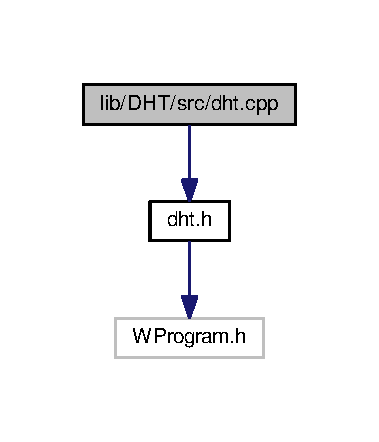
\includegraphics[width=182pt]{dht_8cpp__incl}
\end{center}
\end{figure}
\subsection*{Macros}
\begin{DoxyCompactItemize}
\item 
\#define \hyperlink{dht_8cpp_ae5d44a5fa9fd9d113f6bff639f06ddd6}{M\+I\+N\+\_\+\+I\+N\+T\+E\+R\+V\+AL}~2000
\end{DoxyCompactItemize}


\subsection{Macro Definition Documentation}
\index{dht.\+cpp@{dht.\+cpp}!M\+I\+N\+\_\+\+I\+N\+T\+E\+R\+V\+AL@{M\+I\+N\+\_\+\+I\+N\+T\+E\+R\+V\+AL}}
\index{M\+I\+N\+\_\+\+I\+N\+T\+E\+R\+V\+AL@{M\+I\+N\+\_\+\+I\+N\+T\+E\+R\+V\+AL}!dht.\+cpp@{dht.\+cpp}}
\subsubsection[{\texorpdfstring{M\+I\+N\+\_\+\+I\+N\+T\+E\+R\+V\+AL}{MIN_INTERVAL}}]{\setlength{\rightskip}{0pt plus 5cm}\#define M\+I\+N\+\_\+\+I\+N\+T\+E\+R\+V\+AL~2000}\hypertarget{dht_8cpp_ae5d44a5fa9fd9d113f6bff639f06ddd6}{}\label{dht_8cpp_ae5d44a5fa9fd9d113f6bff639f06ddd6}


Definition at line 9 of file dht.\+cpp.


\hypertarget{dht_8h}{}\section{lib/\+D\+H\+T/dht.h File Reference}
\label{dht_8h}\index{lib/\+D\+H\+T/dht.\+h@{lib/\+D\+H\+T/dht.\+h}}
{\ttfamily \#include $<$W\+Program.\+h$>$}\\*
{\ttfamily \#include $<$pins\+\_\+arduino.\+h$>$}\\*
Include dependency graph for dht.\+h\+:
% FIG 0
This graph shows which files directly or indirectly include this file\+:
% FIG 1
\subsection*{Classes}
\begin{DoxyCompactItemize}
\item 
class \hyperlink{classdht}{dht}
\end{DoxyCompactItemize}
\subsection*{Macros}
\begin{DoxyCompactItemize}
\item 
\#define \hyperlink{dht_8h_a981ffad927ef4f937207f4374cf33e1c}{D\+H\+T\+\_\+\+L\+I\+B\+\_\+\+V\+E\+R\+S\+I\+ON}~\char`\"{}0.\+1.\+21\char`\"{}
\item 
\#define \hyperlink{dht_8h_ab1b9cb0b80df3b9e1268f0e13ae80e11}{D\+H\+T\+L\+I\+B\+\_\+\+OK}~0
\item 
\#define \hyperlink{dht_8h_acda0653986ebb86e8bfed007bbf6a059}{D\+H\+T\+L\+I\+B\+\_\+\+E\+R\+R\+O\+R\+\_\+\+C\+H\+E\+C\+K\+S\+UM}~-\/1
\item 
\#define \hyperlink{dht_8h_ad6f86a85e5e1342005c23ceac36ec192}{D\+H\+T\+L\+I\+B\+\_\+\+E\+R\+R\+O\+R\+\_\+\+T\+I\+M\+E\+O\+UT}~-\/2
\item 
\#define \hyperlink{dht_8h_abc3e2e3759c80a2d31a059930990f49b}{D\+H\+T\+L\+I\+B\+\_\+\+E\+R\+R\+O\+R\+\_\+\+C\+O\+N\+N\+E\+CT}~-\/3
\item 
\#define \hyperlink{dht_8h_a6183db22278ba6596cd3d5aa26fb3b53}{D\+H\+T\+L\+I\+B\+\_\+\+E\+R\+R\+O\+R\+\_\+\+A\+C\+K\+\_\+L}~-\/4
\item 
\#define \hyperlink{dht_8h_adc68fb358de41083fe47747a8702cc35}{D\+H\+T\+L\+I\+B\+\_\+\+E\+R\+R\+O\+R\+\_\+\+A\+C\+K\+\_\+H}~-\/5
\item 
\#define \hyperlink{dht_8h_a5d7db73dafb20a282eb84d84778d3ee3}{D\+H\+T\+L\+I\+B\+\_\+\+D\+H\+T11\+\_\+\+W\+A\+K\+E\+UP}~18
\item 
\#define \hyperlink{dht_8h_ad4e4ae0f10e2d27eb4229474a55aadcb}{D\+H\+T\+L\+I\+B\+\_\+\+D\+H\+T\+\_\+\+W\+A\+K\+E\+UP}~1
\item 
\#define \hyperlink{dht_8h_a3715db703c7182b74af1d672b85e245b}{D\+H\+T\+L\+I\+B\+\_\+\+D\+H\+T11\+\_\+\+L\+E\+A\+D\+I\+N\+G\+\_\+\+Z\+E\+R\+OS}~1
\item 
\#define \hyperlink{dht_8h_a756c4be0b03863e3b04747e5fba12f87}{D\+H\+T\+L\+I\+B\+\_\+\+D\+H\+T\+\_\+\+L\+E\+A\+D\+I\+N\+G\+\_\+\+Z\+E\+R\+OS}~6
\item 
\#define \hyperlink{dht_8h_ad0e2e9ddfb66fe5e0727b63c7313ddf3}{D\+H\+T\+L\+I\+B\+\_\+\+T\+I\+M\+E\+O\+UT}~1000
\end{DoxyCompactItemize}


\subsection{Macro Definition Documentation}
\index{dht.\+h@{dht.\+h}!D\+H\+T\+\_\+\+L\+I\+B\+\_\+\+V\+E\+R\+S\+I\+ON@{D\+H\+T\+\_\+\+L\+I\+B\+\_\+\+V\+E\+R\+S\+I\+ON}}
\index{D\+H\+T\+\_\+\+L\+I\+B\+\_\+\+V\+E\+R\+S\+I\+ON@{D\+H\+T\+\_\+\+L\+I\+B\+\_\+\+V\+E\+R\+S\+I\+ON}!dht.\+h@{dht.\+h}}
\subsubsection[{\texorpdfstring{D\+H\+T\+\_\+\+L\+I\+B\+\_\+\+V\+E\+R\+S\+I\+ON}{DHT_LIB_VERSION}}]{\setlength{\rightskip}{0pt plus 5cm}\#define D\+H\+T\+\_\+\+L\+I\+B\+\_\+\+V\+E\+R\+S\+I\+ON~\char`\"{}0.\+1.\+21\char`\"{}}\hypertarget{dht_8h_a981ffad927ef4f937207f4374cf33e1c}{}\label{dht_8h_a981ffad927ef4f937207f4374cf33e1c}


Definition at line 22 of file dht.\+h.

\index{dht.\+h@{dht.\+h}!D\+H\+T\+L\+I\+B\+\_\+\+D\+H\+T11\+\_\+\+L\+E\+A\+D\+I\+N\+G\+\_\+\+Z\+E\+R\+OS@{D\+H\+T\+L\+I\+B\+\_\+\+D\+H\+T11\+\_\+\+L\+E\+A\+D\+I\+N\+G\+\_\+\+Z\+E\+R\+OS}}
\index{D\+H\+T\+L\+I\+B\+\_\+\+D\+H\+T11\+\_\+\+L\+E\+A\+D\+I\+N\+G\+\_\+\+Z\+E\+R\+OS@{D\+H\+T\+L\+I\+B\+\_\+\+D\+H\+T11\+\_\+\+L\+E\+A\+D\+I\+N\+G\+\_\+\+Z\+E\+R\+OS}!dht.\+h@{dht.\+h}}
\subsubsection[{\texorpdfstring{D\+H\+T\+L\+I\+B\+\_\+\+D\+H\+T11\+\_\+\+L\+E\+A\+D\+I\+N\+G\+\_\+\+Z\+E\+R\+OS}{DHTLIB_DHT11_LEADING_ZEROS}}]{\setlength{\rightskip}{0pt plus 5cm}\#define D\+H\+T\+L\+I\+B\+\_\+\+D\+H\+T11\+\_\+\+L\+E\+A\+D\+I\+N\+G\+\_\+\+Z\+E\+R\+OS~1}\hypertarget{dht_8h_a3715db703c7182b74af1d672b85e245b}{}\label{dht_8h_a3715db703c7182b74af1d672b85e245b}


Definition at line 34 of file dht.\+h.

\index{dht.\+h@{dht.\+h}!D\+H\+T\+L\+I\+B\+\_\+\+D\+H\+T11\+\_\+\+W\+A\+K\+E\+UP@{D\+H\+T\+L\+I\+B\+\_\+\+D\+H\+T11\+\_\+\+W\+A\+K\+E\+UP}}
\index{D\+H\+T\+L\+I\+B\+\_\+\+D\+H\+T11\+\_\+\+W\+A\+K\+E\+UP@{D\+H\+T\+L\+I\+B\+\_\+\+D\+H\+T11\+\_\+\+W\+A\+K\+E\+UP}!dht.\+h@{dht.\+h}}
\subsubsection[{\texorpdfstring{D\+H\+T\+L\+I\+B\+\_\+\+D\+H\+T11\+\_\+\+W\+A\+K\+E\+UP}{DHTLIB_DHT11_WAKEUP}}]{\setlength{\rightskip}{0pt plus 5cm}\#define D\+H\+T\+L\+I\+B\+\_\+\+D\+H\+T11\+\_\+\+W\+A\+K\+E\+UP~18}\hypertarget{dht_8h_a5d7db73dafb20a282eb84d84778d3ee3}{}\label{dht_8h_a5d7db73dafb20a282eb84d84778d3ee3}


Definition at line 31 of file dht.\+h.

\index{dht.\+h@{dht.\+h}!D\+H\+T\+L\+I\+B\+\_\+\+D\+H\+T\+\_\+\+L\+E\+A\+D\+I\+N\+G\+\_\+\+Z\+E\+R\+OS@{D\+H\+T\+L\+I\+B\+\_\+\+D\+H\+T\+\_\+\+L\+E\+A\+D\+I\+N\+G\+\_\+\+Z\+E\+R\+OS}}
\index{D\+H\+T\+L\+I\+B\+\_\+\+D\+H\+T\+\_\+\+L\+E\+A\+D\+I\+N\+G\+\_\+\+Z\+E\+R\+OS@{D\+H\+T\+L\+I\+B\+\_\+\+D\+H\+T\+\_\+\+L\+E\+A\+D\+I\+N\+G\+\_\+\+Z\+E\+R\+OS}!dht.\+h@{dht.\+h}}
\subsubsection[{\texorpdfstring{D\+H\+T\+L\+I\+B\+\_\+\+D\+H\+T\+\_\+\+L\+E\+A\+D\+I\+N\+G\+\_\+\+Z\+E\+R\+OS}{DHTLIB_DHT_LEADING_ZEROS}}]{\setlength{\rightskip}{0pt plus 5cm}\#define D\+H\+T\+L\+I\+B\+\_\+\+D\+H\+T\+\_\+\+L\+E\+A\+D\+I\+N\+G\+\_\+\+Z\+E\+R\+OS~6}\hypertarget{dht_8h_a756c4be0b03863e3b04747e5fba12f87}{}\label{dht_8h_a756c4be0b03863e3b04747e5fba12f87}


Definition at line 35 of file dht.\+h.

\index{dht.\+h@{dht.\+h}!D\+H\+T\+L\+I\+B\+\_\+\+D\+H\+T\+\_\+\+W\+A\+K\+E\+UP@{D\+H\+T\+L\+I\+B\+\_\+\+D\+H\+T\+\_\+\+W\+A\+K\+E\+UP}}
\index{D\+H\+T\+L\+I\+B\+\_\+\+D\+H\+T\+\_\+\+W\+A\+K\+E\+UP@{D\+H\+T\+L\+I\+B\+\_\+\+D\+H\+T\+\_\+\+W\+A\+K\+E\+UP}!dht.\+h@{dht.\+h}}
\subsubsection[{\texorpdfstring{D\+H\+T\+L\+I\+B\+\_\+\+D\+H\+T\+\_\+\+W\+A\+K\+E\+UP}{DHTLIB_DHT_WAKEUP}}]{\setlength{\rightskip}{0pt plus 5cm}\#define D\+H\+T\+L\+I\+B\+\_\+\+D\+H\+T\+\_\+\+W\+A\+K\+E\+UP~1}\hypertarget{dht_8h_ad4e4ae0f10e2d27eb4229474a55aadcb}{}\label{dht_8h_ad4e4ae0f10e2d27eb4229474a55aadcb}


Definition at line 32 of file dht.\+h.

\index{dht.\+h@{dht.\+h}!D\+H\+T\+L\+I\+B\+\_\+\+E\+R\+R\+O\+R\+\_\+\+A\+C\+K\+\_\+H@{D\+H\+T\+L\+I\+B\+\_\+\+E\+R\+R\+O\+R\+\_\+\+A\+C\+K\+\_\+H}}
\index{D\+H\+T\+L\+I\+B\+\_\+\+E\+R\+R\+O\+R\+\_\+\+A\+C\+K\+\_\+H@{D\+H\+T\+L\+I\+B\+\_\+\+E\+R\+R\+O\+R\+\_\+\+A\+C\+K\+\_\+H}!dht.\+h@{dht.\+h}}
\subsubsection[{\texorpdfstring{D\+H\+T\+L\+I\+B\+\_\+\+E\+R\+R\+O\+R\+\_\+\+A\+C\+K\+\_\+H}{DHTLIB_ERROR_ACK_H}}]{\setlength{\rightskip}{0pt plus 5cm}\#define D\+H\+T\+L\+I\+B\+\_\+\+E\+R\+R\+O\+R\+\_\+\+A\+C\+K\+\_\+H~-\/5}\hypertarget{dht_8h_adc68fb358de41083fe47747a8702cc35}{}\label{dht_8h_adc68fb358de41083fe47747a8702cc35}


Definition at line 29 of file dht.\+h.

\index{dht.\+h@{dht.\+h}!D\+H\+T\+L\+I\+B\+\_\+\+E\+R\+R\+O\+R\+\_\+\+A\+C\+K\+\_\+L@{D\+H\+T\+L\+I\+B\+\_\+\+E\+R\+R\+O\+R\+\_\+\+A\+C\+K\+\_\+L}}
\index{D\+H\+T\+L\+I\+B\+\_\+\+E\+R\+R\+O\+R\+\_\+\+A\+C\+K\+\_\+L@{D\+H\+T\+L\+I\+B\+\_\+\+E\+R\+R\+O\+R\+\_\+\+A\+C\+K\+\_\+L}!dht.\+h@{dht.\+h}}
\subsubsection[{\texorpdfstring{D\+H\+T\+L\+I\+B\+\_\+\+E\+R\+R\+O\+R\+\_\+\+A\+C\+K\+\_\+L}{DHTLIB_ERROR_ACK_L}}]{\setlength{\rightskip}{0pt plus 5cm}\#define D\+H\+T\+L\+I\+B\+\_\+\+E\+R\+R\+O\+R\+\_\+\+A\+C\+K\+\_\+L~-\/4}\hypertarget{dht_8h_a6183db22278ba6596cd3d5aa26fb3b53}{}\label{dht_8h_a6183db22278ba6596cd3d5aa26fb3b53}


Definition at line 28 of file dht.\+h.

\index{dht.\+h@{dht.\+h}!D\+H\+T\+L\+I\+B\+\_\+\+E\+R\+R\+O\+R\+\_\+\+C\+H\+E\+C\+K\+S\+UM@{D\+H\+T\+L\+I\+B\+\_\+\+E\+R\+R\+O\+R\+\_\+\+C\+H\+E\+C\+K\+S\+UM}}
\index{D\+H\+T\+L\+I\+B\+\_\+\+E\+R\+R\+O\+R\+\_\+\+C\+H\+E\+C\+K\+S\+UM@{D\+H\+T\+L\+I\+B\+\_\+\+E\+R\+R\+O\+R\+\_\+\+C\+H\+E\+C\+K\+S\+UM}!dht.\+h@{dht.\+h}}
\subsubsection[{\texorpdfstring{D\+H\+T\+L\+I\+B\+\_\+\+E\+R\+R\+O\+R\+\_\+\+C\+H\+E\+C\+K\+S\+UM}{DHTLIB_ERROR_CHECKSUM}}]{\setlength{\rightskip}{0pt plus 5cm}\#define D\+H\+T\+L\+I\+B\+\_\+\+E\+R\+R\+O\+R\+\_\+\+C\+H\+E\+C\+K\+S\+UM~-\/1}\hypertarget{dht_8h_acda0653986ebb86e8bfed007bbf6a059}{}\label{dht_8h_acda0653986ebb86e8bfed007bbf6a059}


Definition at line 25 of file dht.\+h.

\index{dht.\+h@{dht.\+h}!D\+H\+T\+L\+I\+B\+\_\+\+E\+R\+R\+O\+R\+\_\+\+C\+O\+N\+N\+E\+CT@{D\+H\+T\+L\+I\+B\+\_\+\+E\+R\+R\+O\+R\+\_\+\+C\+O\+N\+N\+E\+CT}}
\index{D\+H\+T\+L\+I\+B\+\_\+\+E\+R\+R\+O\+R\+\_\+\+C\+O\+N\+N\+E\+CT@{D\+H\+T\+L\+I\+B\+\_\+\+E\+R\+R\+O\+R\+\_\+\+C\+O\+N\+N\+E\+CT}!dht.\+h@{dht.\+h}}
\subsubsection[{\texorpdfstring{D\+H\+T\+L\+I\+B\+\_\+\+E\+R\+R\+O\+R\+\_\+\+C\+O\+N\+N\+E\+CT}{DHTLIB_ERROR_CONNECT}}]{\setlength{\rightskip}{0pt plus 5cm}\#define D\+H\+T\+L\+I\+B\+\_\+\+E\+R\+R\+O\+R\+\_\+\+C\+O\+N\+N\+E\+CT~-\/3}\hypertarget{dht_8h_abc3e2e3759c80a2d31a059930990f49b}{}\label{dht_8h_abc3e2e3759c80a2d31a059930990f49b}


Definition at line 27 of file dht.\+h.

\index{dht.\+h@{dht.\+h}!D\+H\+T\+L\+I\+B\+\_\+\+E\+R\+R\+O\+R\+\_\+\+T\+I\+M\+E\+O\+UT@{D\+H\+T\+L\+I\+B\+\_\+\+E\+R\+R\+O\+R\+\_\+\+T\+I\+M\+E\+O\+UT}}
\index{D\+H\+T\+L\+I\+B\+\_\+\+E\+R\+R\+O\+R\+\_\+\+T\+I\+M\+E\+O\+UT@{D\+H\+T\+L\+I\+B\+\_\+\+E\+R\+R\+O\+R\+\_\+\+T\+I\+M\+E\+O\+UT}!dht.\+h@{dht.\+h}}
\subsubsection[{\texorpdfstring{D\+H\+T\+L\+I\+B\+\_\+\+E\+R\+R\+O\+R\+\_\+\+T\+I\+M\+E\+O\+UT}{DHTLIB_ERROR_TIMEOUT}}]{\setlength{\rightskip}{0pt plus 5cm}\#define D\+H\+T\+L\+I\+B\+\_\+\+E\+R\+R\+O\+R\+\_\+\+T\+I\+M\+E\+O\+UT~-\/2}\hypertarget{dht_8h_ad6f86a85e5e1342005c23ceac36ec192}{}\label{dht_8h_ad6f86a85e5e1342005c23ceac36ec192}


Definition at line 26 of file dht.\+h.

\index{dht.\+h@{dht.\+h}!D\+H\+T\+L\+I\+B\+\_\+\+OK@{D\+H\+T\+L\+I\+B\+\_\+\+OK}}
\index{D\+H\+T\+L\+I\+B\+\_\+\+OK@{D\+H\+T\+L\+I\+B\+\_\+\+OK}!dht.\+h@{dht.\+h}}
\subsubsection[{\texorpdfstring{D\+H\+T\+L\+I\+B\+\_\+\+OK}{DHTLIB_OK}}]{\setlength{\rightskip}{0pt plus 5cm}\#define D\+H\+T\+L\+I\+B\+\_\+\+OK~0}\hypertarget{dht_8h_ab1b9cb0b80df3b9e1268f0e13ae80e11}{}\label{dht_8h_ab1b9cb0b80df3b9e1268f0e13ae80e11}


Definition at line 24 of file dht.\+h.

\index{dht.\+h@{dht.\+h}!D\+H\+T\+L\+I\+B\+\_\+\+T\+I\+M\+E\+O\+UT@{D\+H\+T\+L\+I\+B\+\_\+\+T\+I\+M\+E\+O\+UT}}
\index{D\+H\+T\+L\+I\+B\+\_\+\+T\+I\+M\+E\+O\+UT@{D\+H\+T\+L\+I\+B\+\_\+\+T\+I\+M\+E\+O\+UT}!dht.\+h@{dht.\+h}}
\subsubsection[{\texorpdfstring{D\+H\+T\+L\+I\+B\+\_\+\+T\+I\+M\+E\+O\+UT}{DHTLIB_TIMEOUT}}]{\setlength{\rightskip}{0pt plus 5cm}\#define D\+H\+T\+L\+I\+B\+\_\+\+T\+I\+M\+E\+O\+UT~1000}\hypertarget{dht_8h_ad0e2e9ddfb66fe5e0727b63c7313ddf3}{}\label{dht_8h_ad0e2e9ddfb66fe5e0727b63c7313ddf3}


Definition at line 43 of file dht.\+h.


\hypertarget{ldr_8cpp}{}\section{lib/\+L\+D\+R/src/ldr.cpp File Reference}
\label{ldr_8cpp}\index{lib/\+L\+D\+R/src/ldr.\+cpp@{lib/\+L\+D\+R/src/ldr.\+cpp}}
{\ttfamily \#include $<$Arduino.\+h$>$}\\*
{\ttfamily \#include \char`\"{}ldr.\+hpp\char`\"{}}\\*
Include dependency graph for ldr.\+cpp\+:\nopagebreak
\begin{figure}[H]
\begin{center}
\leavevmode
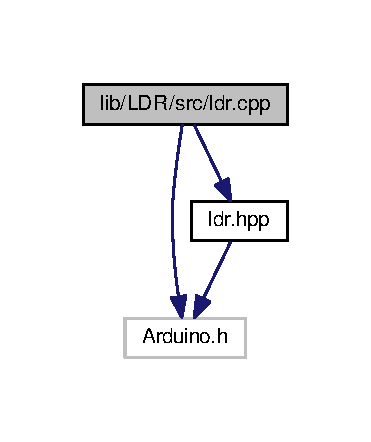
\includegraphics[width=178pt]{ldr_8cpp__incl}
\end{center}
\end{figure}

\hypertarget{ldr_8hpp}{}\section{lib/\+L\+D\+R/src/ldr.hpp File Reference}
\label{ldr_8hpp}\index{lib/\+L\+D\+R/src/ldr.\+hpp@{lib/\+L\+D\+R/src/ldr.\+hpp}}
{\ttfamily \#include $<$Arduino.\+h$>$}\\*
Include dependency graph for ldr.\+hpp\+:
% FIG 0
This graph shows which files directly or indirectly include this file\+:
% FIG 1
\subsection*{Classes}
\begin{DoxyCompactItemize}
\item 
class \hyperlink{classldr}{ldr}
\end{DoxyCompactItemize}

\hypertarget{_log_manager_8cpp}{}\section{lib/\+Log\+Manager/src/\+Log\+Manager.cpp File Reference}
\label{_log_manager_8cpp}\index{lib/\+Log\+Manager/src/\+Log\+Manager.\+cpp@{lib/\+Log\+Manager/src/\+Log\+Manager.\+cpp}}
{\ttfamily \#include $<$Arduino.\+h$>$}\\*
{\ttfamily \#include \char`\"{}Log\+Manager.\+hpp\char`\"{}}\\*
Include dependency graph for Log\+Manager.\+cpp\+:\nopagebreak
\begin{figure}[H]
\begin{center}
\leavevmode
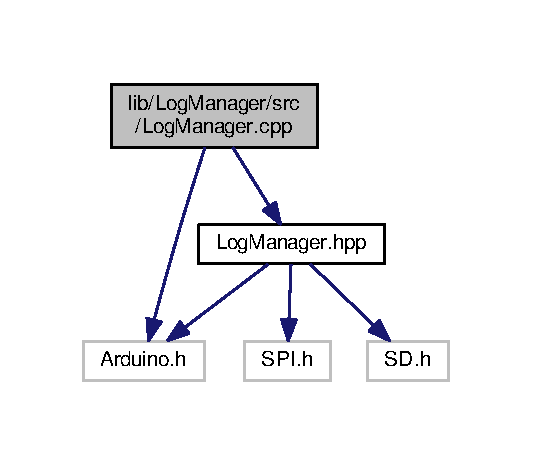
\includegraphics[width=256pt]{_log_manager_8cpp__incl}
\end{center}
\end{figure}

\hypertarget{_log_manager_8hpp}{}\section{lib/\+Log\+Manager/src/\+Log\+Manager.hpp File Reference}
\label{_log_manager_8hpp}\index{lib/\+Log\+Manager/src/\+Log\+Manager.\+hpp@{lib/\+Log\+Manager/src/\+Log\+Manager.\+hpp}}
{\ttfamily \#include $<$Arduino.\+h$>$}\\*
{\ttfamily \#include $<$S\+P\+I.\+h$>$}\\*
{\ttfamily \#include $<$S\+D.\+h$>$}\\*
Include dependency graph for Log\+Manager.\+hpp\+:\nopagebreak
\begin{figure}[H]
\begin{center}
\leavevmode
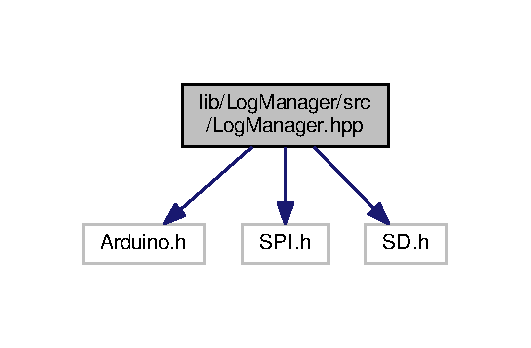
\includegraphics[width=255pt]{_log_manager_8hpp__incl}
\end{center}
\end{figure}
This graph shows which files directly or indirectly include this file\+:\nopagebreak
\begin{figure}[H]
\begin{center}
\leavevmode
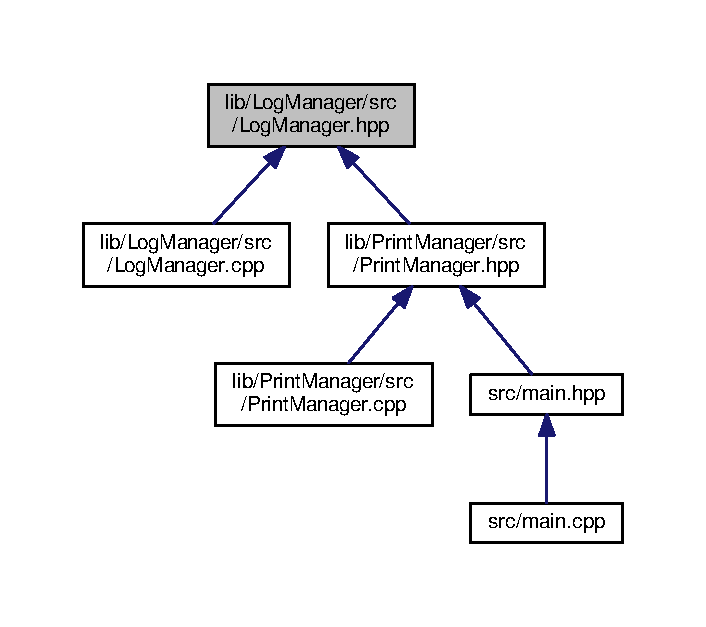
\includegraphics[width=339pt]{_log_manager_8hpp__dep__incl}
\end{center}
\end{figure}
\subsection*{Classes}
\begin{DoxyCompactItemize}
\item 
class \hyperlink{class_log_manager}{Log\+Manager}
\end{DoxyCompactItemize}
\subsection*{Enumerations}
\begin{DoxyCompactItemize}
\item 
enum \hyperlink{_log_manager_8hpp_abe4bda5900ce4ef9e328ebb5e097a8a1}{verbose\+Type} \+: const uint8\+\_\+t 
\end{DoxyCompactItemize}


\subsection{Enumeration Type Documentation}
\index{Log\+Manager.\+hpp@{Log\+Manager.\+hpp}!verbose\+Type@{verbose\+Type}}
\index{verbose\+Type@{verbose\+Type}!Log\+Manager.\+hpp@{Log\+Manager.\+hpp}}
\subsubsection[{\texorpdfstring{verbose\+Type}{verboseType}}]{\setlength{\rightskip}{0pt plus 5cm}enum {\bf verbose\+Type} \+: const uint8\+\_\+t}\hypertarget{_log_manager_8hpp_abe4bda5900ce4ef9e328ebb5e097a8a1}{}\label{_log_manager_8hpp_abe4bda5900ce4ef9e328ebb5e097a8a1}


Definition at line 9 of file Log\+Manager.\+hpp.


\hypertarget{_m_q_sensor_8cpp}{}\section{lib/\+M\+Q-\/\+Sensor/src/\+M\+Q\+Sensor.cpp File Reference}
\label{_m_q_sensor_8cpp}\index{lib/\+M\+Q-\/\+Sensor/src/\+M\+Q\+Sensor.\+cpp@{lib/\+M\+Q-\/\+Sensor/src/\+M\+Q\+Sensor.\+cpp}}
{\ttfamily \#include $<$Arduino.\+h$>$}\\*
{\ttfamily \#include \char`\"{}M\+Q\+Sensor.\+hpp\char`\"{}}\\*
Include dependency graph for M\+Q\+Sensor.\+cpp\+:\nopagebreak
\begin{figure}[H]
\begin{center}
\leavevmode
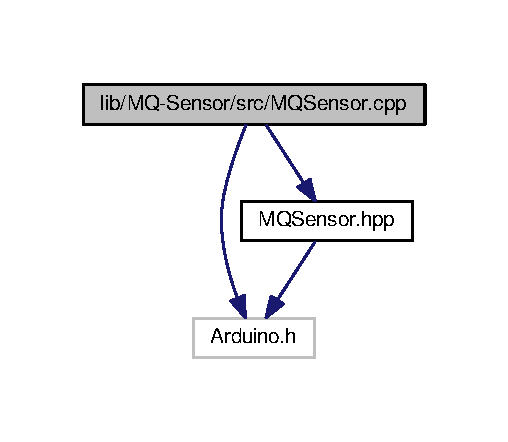
\includegraphics[width=244pt]{_m_q_sensor_8cpp__incl}
\end{center}
\end{figure}
\subsection*{Functions}
\begin{DoxyCompactItemize}
\item 
{\footnotesize template$<$typename T $>$ }\\T \hyperlink{_m_q_sensor_8cpp_a93e58338e8b2c1f572bbcccb7eff9714}{map} (T x, T in\+\_\+min, T in\+\_\+max, T out\+\_\+min, T out\+\_\+max)
\end{DoxyCompactItemize}


\subsection{Function Documentation}
\index{M\+Q\+Sensor.\+cpp@{M\+Q\+Sensor.\+cpp}!map@{map}}
\index{map@{map}!M\+Q\+Sensor.\+cpp@{M\+Q\+Sensor.\+cpp}}
\subsubsection[{\texorpdfstring{map(\+T x, T in\+\_\+min, T in\+\_\+max, T out\+\_\+min, T out\+\_\+max)}{map(T x, T in_min, T in_max, T out_min, T out_max)}}]{\setlength{\rightskip}{0pt plus 5cm}template$<$typename T $>$ T map (
\begin{DoxyParamCaption}
\item[{T}]{x, }
\item[{T}]{in\+\_\+min, }
\item[{T}]{in\+\_\+max, }
\item[{T}]{out\+\_\+min, }
\item[{T}]{out\+\_\+max}
\end{DoxyParamCaption}
)}\hypertarget{_m_q_sensor_8cpp_a93e58338e8b2c1f572bbcccb7eff9714}{}\label{_m_q_sensor_8cpp_a93e58338e8b2c1f572bbcccb7eff9714}
Re-\/maps a number from one range to another. That is, a value of in\+\_\+min would get mapped to out\+\_\+min, a value of in\+\_\+max to out\+\_\+max, values in-\/between to values in-\/between, etc. 
\begin{DoxyParams}{Parameters}
{\em x} & The value to be mapped. \\
\hline
{\em in\+\_\+min} & The lower bond of the value\textquotesingle{}s current range. \\
\hline
{\em in\+\_\+max} & The upper bond of the value\textquotesingle{}s current range. \\
\hline
{\em out\+\_\+min} & The lower bond of the value\textquotesingle{}s target range. \\
\hline
{\em out\+\_\+max} & The upper bond of the value\textquotesingle{}s target range. \\
\hline
\end{DoxyParams}
\begin{DoxyReturn}{Returns}
The mapped value. 
\end{DoxyReturn}


Definition at line 26 of file M\+Q\+Sensor.\+cpp.


\hypertarget{_m_q_sensor_8hpp}{}\section{lib/\+M\+Q-\/\+Sensor/src/\+M\+Q\+Sensor.hpp File Reference}
\label{_m_q_sensor_8hpp}\index{lib/\+M\+Q-\/\+Sensor/src/\+M\+Q\+Sensor.\+hpp@{lib/\+M\+Q-\/\+Sensor/src/\+M\+Q\+Sensor.\+hpp}}
{\ttfamily \#include $<$Arduino.\+h$>$}\\*
Include dependency graph for M\+Q\+Sensor.\+hpp\+:\nopagebreak
\begin{figure}[H]
\begin{center}
\leavevmode
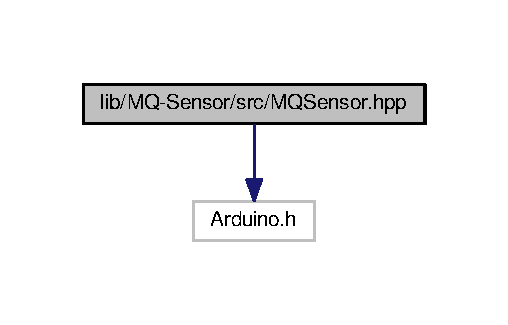
\includegraphics[width=244pt]{_m_q_sensor_8hpp__incl}
\end{center}
\end{figure}
This graph shows which files directly or indirectly include this file\+:\nopagebreak
\begin{figure}[H]
\begin{center}
\leavevmode
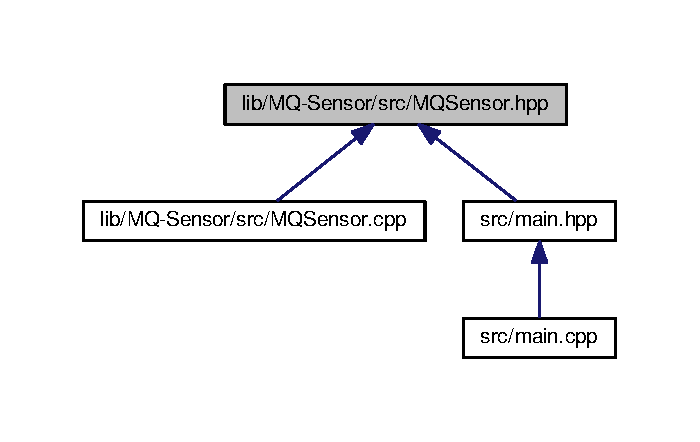
\includegraphics[width=336pt]{_m_q_sensor_8hpp__dep__incl}
\end{center}
\end{figure}
\subsection*{Classes}
\begin{DoxyCompactItemize}
\item 
class \hyperlink{class_m_q_sensor}{M\+Q\+Sensor}
\item 
class \hyperlink{class_m_q_dummy}{M\+Q\+Dummy}
\item 
class \hyperlink{class_m_q_potentiometer}{M\+Q\+Potentiometer}
\item 
class \hyperlink{class_m_q3}{M\+Q3}
\item 
class \hyperlink{class_m_q7}{M\+Q7}
\end{DoxyCompactItemize}
\subsection*{Enumerations}
\begin{DoxyCompactItemize}
\item 
enum \hyperlink{_m_q_sensor_8hpp_aa39cce9d2f2c6464e774b8f5684bd664}{S\+E\+N\+S\+O\+R\+\_\+\+T\+Y\+PE} \+: const uint8\+\_\+t 
\item 
enum \hyperlink{_m_q_sensor_8hpp_adc1ba5bd8d887ddb6973cff15d9a1501}{G\+A\+S\+\_\+\+T\+Y\+PE} \+: const uint8\+\_\+t 
\end{DoxyCompactItemize}


\subsection{Enumeration Type Documentation}
\index{M\+Q\+Sensor.\+hpp@{M\+Q\+Sensor.\+hpp}!G\+A\+S\+\_\+\+T\+Y\+PE@{G\+A\+S\+\_\+\+T\+Y\+PE}}
\index{G\+A\+S\+\_\+\+T\+Y\+PE@{G\+A\+S\+\_\+\+T\+Y\+PE}!M\+Q\+Sensor.\+hpp@{M\+Q\+Sensor.\+hpp}}
\subsubsection[{\texorpdfstring{G\+A\+S\+\_\+\+T\+Y\+PE}{GAS_TYPE}}]{\setlength{\rightskip}{0pt plus 5cm}enum {\bf G\+A\+S\+\_\+\+T\+Y\+PE} \+: const uint8\+\_\+t}\hypertarget{_m_q_sensor_8hpp_adc1ba5bd8d887ddb6973cff15d9a1501}{}\label{_m_q_sensor_8hpp_adc1ba5bd8d887ddb6973cff15d9a1501}


Definition at line 29 of file M\+Q\+Sensor.\+hpp.

\index{M\+Q\+Sensor.\+hpp@{M\+Q\+Sensor.\+hpp}!S\+E\+N\+S\+O\+R\+\_\+\+T\+Y\+PE@{S\+E\+N\+S\+O\+R\+\_\+\+T\+Y\+PE}}
\index{S\+E\+N\+S\+O\+R\+\_\+\+T\+Y\+PE@{S\+E\+N\+S\+O\+R\+\_\+\+T\+Y\+PE}!M\+Q\+Sensor.\+hpp@{M\+Q\+Sensor.\+hpp}}
\subsubsection[{\texorpdfstring{S\+E\+N\+S\+O\+R\+\_\+\+T\+Y\+PE}{SENSOR_TYPE}}]{\setlength{\rightskip}{0pt plus 5cm}enum {\bf S\+E\+N\+S\+O\+R\+\_\+\+T\+Y\+PE} \+: const uint8\+\_\+t}\hypertarget{_m_q_sensor_8hpp_aa39cce9d2f2c6464e774b8f5684bd664}{}\label{_m_q_sensor_8hpp_aa39cce9d2f2c6464e774b8f5684bd664}


Definition at line 15 of file M\+Q\+Sensor.\+hpp.


\hypertarget{_print_manager_8cpp}{}\section{lib/\+Print\+Manager/src/\+Print\+Manager.cpp File Reference}
\label{_print_manager_8cpp}\index{lib/\+Print\+Manager/src/\+Print\+Manager.\+cpp@{lib/\+Print\+Manager/src/\+Print\+Manager.\+cpp}}
{\ttfamily \#include $<$Arduino.\+h$>$}\\*
{\ttfamily \#include \char`\"{}Print\+Manager.\+hpp\char`\"{}}\\*
Include dependency graph for Print\+Manager.\+cpp\+:\nopagebreak
\begin{figure}[H]
\begin{center}
\leavevmode
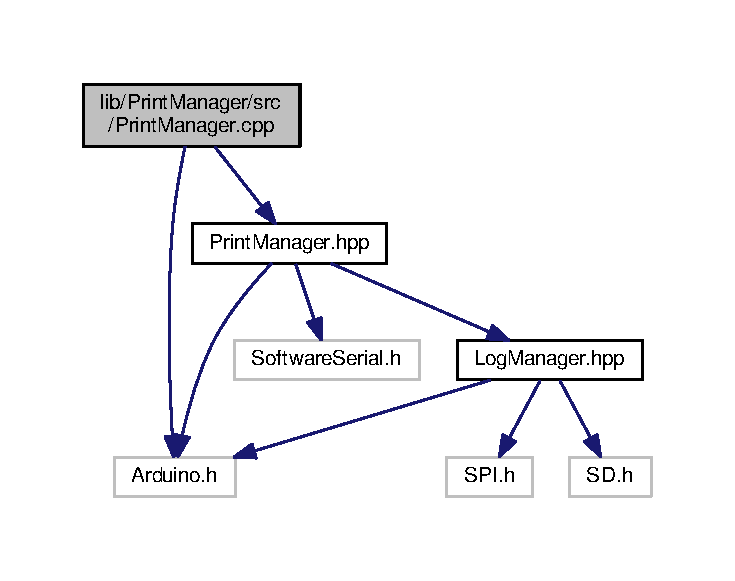
\includegraphics[width=350pt]{_print_manager_8cpp__incl}
\end{center}
\end{figure}
\subsection*{Functions}
\begin{DoxyCompactItemize}
\item 
constexpr int \hyperlink{_print_manager_8cpp_ac56103e1cb66ddb548cc87fa00e0e0c7}{to\+Int} (const char c)
\end{DoxyCompactItemize}


\subsection{Function Documentation}
\index{Print\+Manager.\+cpp@{Print\+Manager.\+cpp}!to\+Int@{to\+Int}}
\index{to\+Int@{to\+Int}!Print\+Manager.\+cpp@{Print\+Manager.\+cpp}}
\subsubsection[{\texorpdfstring{to\+Int(const char c)}{toInt(const char c)}}]{\setlength{\rightskip}{0pt plus 5cm}constexpr int to\+Int (
\begin{DoxyParamCaption}
\item[{const char}]{c}
\end{DoxyParamCaption}
)}\hypertarget{_print_manager_8cpp_ac56103e1cb66ddb548cc87fa00e0e0c7}{}\label{_print_manager_8cpp_ac56103e1cb66ddb548cc87fa00e0e0c7}


Definition at line 4 of file Print\+Manager.\+cpp.


\hypertarget{_print_manager_8hpp}{}\section{lib/\+Print\+Manager/src/\+Print\+Manager.hpp File Reference}
\label{_print_manager_8hpp}\index{lib/\+Print\+Manager/src/\+Print\+Manager.\+hpp@{lib/\+Print\+Manager/src/\+Print\+Manager.\+hpp}}
{\ttfamily \#include $<$Arduino.\+h$>$}\\*
{\ttfamily \#include $<$Software\+Serial.\+h$>$}\\*
{\ttfamily \#include $<$Log\+Manager.\+hpp$>$}\\*
Include dependency graph for Print\+Manager.\+hpp\+:\nopagebreak
\begin{figure}[H]
\begin{center}
\leavevmode
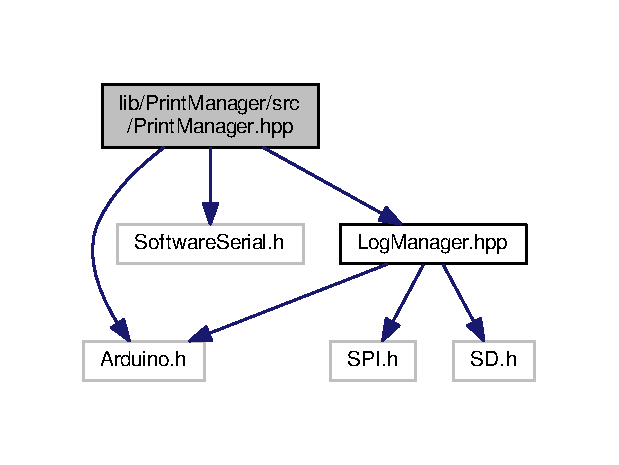
\includegraphics[width=297pt]{_print_manager_8hpp__incl}
\end{center}
\end{figure}
This graph shows which files directly or indirectly include this file\+:\nopagebreak
\begin{figure}[H]
\begin{center}
\leavevmode
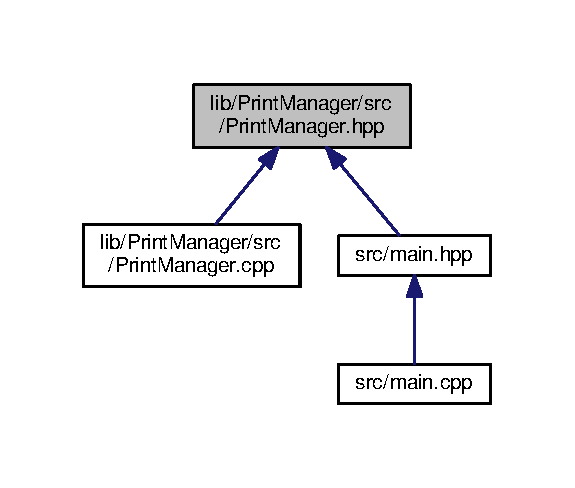
\includegraphics[width=276pt]{_print_manager_8hpp__dep__incl}
\end{center}
\end{figure}
\subsection*{Classes}
\begin{DoxyCompactItemize}
\item 
class \hyperlink{class_print_manager}{Print\+Manager}
\end{DoxyCompactItemize}
\subsection*{Enumerations}
\begin{DoxyCompactItemize}
\item 
enum \hyperlink{_print_manager_8hpp_ac4250c605bd199b412d7419ad514699f}{serial\+Port\+Type} \+: const uint8\+\_\+t 
\end{DoxyCompactItemize}


\subsection{Enumeration Type Documentation}
\index{Print\+Manager.\+hpp@{Print\+Manager.\+hpp}!serial\+Port\+Type@{serial\+Port\+Type}}
\index{serial\+Port\+Type@{serial\+Port\+Type}!Print\+Manager.\+hpp@{Print\+Manager.\+hpp}}
\subsubsection[{\texorpdfstring{serial\+Port\+Type}{serialPortType}}]{\setlength{\rightskip}{0pt plus 5cm}enum {\bf serial\+Port\+Type} \+: const uint8\+\_\+t}\hypertarget{_print_manager_8hpp_ac4250c605bd199b412d7419ad514699f}{}\label{_print_manager_8hpp_ac4250c605bd199b412d7419ad514699f}


Definition at line 9 of file Print\+Manager.\+hpp.


\hypertarget{_8_d_s3231___alarms_8vsarduino_8h}{}\section{lib/\+R\+T\+C/examples/\+D\+S3231\+\_\+\+Alarms/\+Visual Micro/.D\+S3231\+\_\+\+Alarms.\+vsarduino.\+h File Reference}
\label{_8_d_s3231___alarms_8vsarduino_8h}\index{lib/\+R\+T\+C/examples/\+D\+S3231\+\_\+\+Alarms/\+Visual Micro/.\+D\+S3231\+\_\+\+Alarms.\+vsarduino.\+h@{lib/\+R\+T\+C/examples/\+D\+S3231\+\_\+\+Alarms/\+Visual Micro/.\+D\+S3231\+\_\+\+Alarms.\+vsarduino.\+h}}
{\ttfamily \#include $<$arduino.\+h$>$}\\*
{\ttfamily \#include $<$pins\+\_\+arduino.\+h$>$}\\*
{\ttfamily \#include $<$D\+S3231\+\_\+\+Alarms.\+ino$>$}\\*
Include dependency graph for .D\+S3231\+\_\+\+Alarms.\+vsarduino.\+h\+:\nopagebreak
\begin{figure}[H]
\begin{center}
\leavevmode
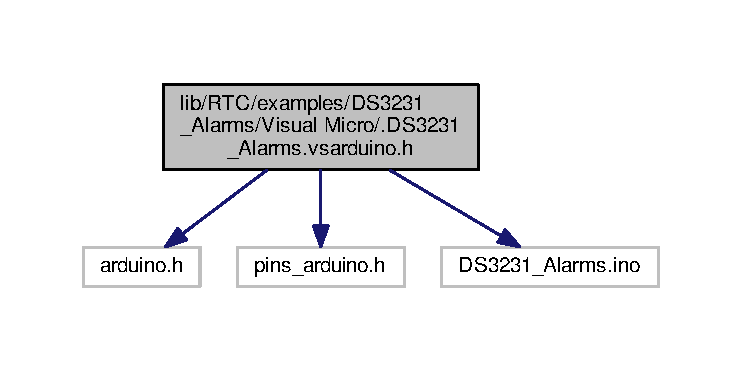
\includegraphics[width=350pt]{_8_d_s3231___alarms_8vsarduino_8h__incl}
\end{center}
\end{figure}
\subsection*{Macros}
\begin{DoxyCompactItemize}
\item 
\#define \hyperlink{_8_d_s3231___alarms_8vsarduino_8h_abf42623921c4853f2e40a168b3b6ea81}{\+\_\+\+\_\+\+A\+V\+R\+\_\+\+A\+Tmega2560\+\_\+\+\_\+}
\item 
\#define \hyperlink{_8_d_s3231___alarms_8vsarduino_8h_a5deccebbf24e21ddc073c8774179f1b3}{A\+R\+D\+U\+I\+NO}~161
\item 
\#define \hyperlink{_8_d_s3231___alarms_8vsarduino_8h_a27a05420b36346cf71496473528b713c}{A\+R\+D\+U\+I\+N\+O\+\_\+\+M\+A\+IN}
\item 
\#define \hyperlink{_8_d_s3231___alarms_8vsarduino_8h_a2c5e50d229c92b7a531ebf48b411457b}{\+\_\+\+\_\+\+A\+V\+R\+\_\+\+\_\+}
\item 
\#define \hyperlink{_8_d_s3231___alarms_8vsarduino_8h_a5ab9a420d5d8dfa81c200a0996ce8b94}{\+\_\+\+\_\+avr\+\_\+\+\_\+}
\item 
\#define \hyperlink{_8_d_s3231___alarms_8vsarduino_8h_a43bafb28b29491ec7f871319b5a3b2f8}{F\+\_\+\+C\+PU}~16000000L
\item 
\#define \hyperlink{_8_d_s3231___alarms_8vsarduino_8h_a1b391bc7ed92f79666c4a5d840aa1edd}{\+\_\+\+\_\+cplusplus}
\item 
\#define \hyperlink{_8_d_s3231___alarms_8vsarduino_8h_adbba0f726fc66d7100916c683b7568ae}{G\+C\+C\+\_\+\+V\+E\+R\+S\+I\+ON}~40801
\item 
\#define \hyperlink{_8_d_s3231___alarms_8vsarduino_8h_ad725ed96de84f96063797de6d7aae75f}{A\+R\+D\+U\+I\+N\+O\+\_\+\+A\+R\+C\+H\+\_\+\+A\+VR}
\item 
\#define \hyperlink{_8_d_s3231___alarms_8vsarduino_8h_a44496c9094fd7e8b544280edff102f57}{A\+R\+D\+U\+I\+N\+O\+\_\+\+A\+V\+R\+\_\+\+M\+E\+G\+A2560}
\item 
\#define \hyperlink{_8_d_s3231___alarms_8vsarduino_8h_a9f04218fe09e6ee659e045b2f11542ed}{\+\_\+\+\_\+inline\+\_\+\+\_\+}
\item 
\#define \hyperlink{_8_d_s3231___alarms_8vsarduino_8h_a2982fd921bfec096f995c53980bcfc19}{\+\_\+\+\_\+asm\+\_\+\+\_\+}(x)
\item 
\#define \hyperlink{_8_d_s3231___alarms_8vsarduino_8h_a586c6a171eb0104d519dc0eda5284ef7}{\+\_\+\+\_\+extension\+\_\+\+\_\+}
\item 
\#define \hyperlink{_8_d_s3231___alarms_8vsarduino_8h_a9f04218fe09e6ee659e045b2f11542ed}{\+\_\+\+\_\+inline\+\_\+\+\_\+}
\item 
\#define \hyperlink{_8_d_s3231___alarms_8vsarduino_8h_a64fa3037957156c60db536aad57ae07e}{\+\_\+\+\_\+volatile\+\_\+\+\_\+}
\item 
\#define \hyperlink{_8_d_s3231___alarms_8vsarduino_8h_adbba0f726fc66d7100916c683b7568ae}{G\+C\+C\+\_\+\+V\+E\+R\+S\+I\+ON}~40801
\item 
\#define \hyperlink{_8_d_s3231___alarms_8vsarduino_8h_a5d3a73f59af1b35c5f1293c9f093ffd0}{volatile}(va\+\_\+arg)
\item 
\#define \hyperlink{_8_d_s3231___alarms_8vsarduino_8h_a9f32dbba97c980059b66f67b17dbec8f}{\+\_\+\+\_\+builtin\+\_\+va\+\_\+start}
\item 
\#define \hyperlink{_8_d_s3231___alarms_8vsarduino_8h_acb0d86a11a00d65bec7aa79527037869}{\+\_\+\+\_\+builtin\+\_\+va\+\_\+end}
\item 
\#define \hyperlink{_8_d_s3231___alarms_8vsarduino_8h_a9d373a9b65ff25b2db84c07394e1c212}{\+\_\+\+\_\+attribute\+\_\+\+\_\+}(x)
\item 
\#define \hyperlink{_8_d_s3231___alarms_8vsarduino_8h_a1b173d22e57d9395897acbd8de62d505}{N\+O\+I\+N\+L\+I\+NE}~\hyperlink{_8_d_s3231___alarms_8vsarduino_8h_a9d373a9b65ff25b2db84c07394e1c212}{\+\_\+\+\_\+attribute\+\_\+\+\_\+}((noinline))
\item 
\#define \hyperlink{_8_d_s3231___alarms_8vsarduino_8h_a814419222e0e391a26e8d6ad96bf4cee}{prog\+\_\+void}
\item 
\#define \hyperlink{_8_d_s3231___alarms_8vsarduino_8h_a84a61d55b7efefabd8419e28f02704f9}{P\+G\+M\+\_\+\+V\+O\+I\+D\+\_\+P}~int
\item 
\#define \hyperlink{_8_d_s3231___alarms_8vsarduino_8h_a03fea404d4dc0ef38df1f4acca6534e1}{N\+E\+W\+\_\+H}
\item 
\#define \hyperlink{_8_d_s3231___alarms_8vsarduino_8h_a2520eacecda4bdd7dafaf12b911626d6}{F}(string\+\_\+literal)~((const \hyperlink{_rtc_date_time_8h_ac0acbe713345b6ba392f37a8f4c8dfb2}{P\+R\+O\+G\+M\+EM} char $\ast$)(string\+\_\+literal))
\item 
\#define \hyperlink{_8_d_s3231___alarms_8vsarduino_8h_a68c330e94fe121eba993e5a5973c3162}{cli}()
\item 
\#define \hyperlink{_8_d_s3231___alarms_8vsarduino_8h_a73084a8bbde259ffae72980354b3f027}{pgm\+\_\+read\+\_\+byte}(address\+\_\+short)
\item 
\#define \hyperlink{_8_d_s3231___alarms_8vsarduino_8h_a32d8ab354156f4b1ffdb77a275ba6223}{pgm\+\_\+read\+\_\+word}(address\+\_\+short)
\item 
\#define \hyperlink{_8_d_s3231___alarms_8vsarduino_8h_a0b2720dce7ee888a59f96970100a505f}{pgm\+\_\+read\+\_\+word2}(address\+\_\+short)
\item 
\#define \hyperlink{_8_d_s3231___alarms_8vsarduino_8h_a695126157083b643a98b9b800e28ac6f}{digital\+Pin\+To\+Port}(P)
\item 
\#define \hyperlink{_8_d_s3231___alarms_8vsarduino_8h_a97d049a432ec5a04c40510df440c786a}{digital\+Pin\+To\+Bit\+Mask}(P)
\item 
\#define \hyperlink{_8_d_s3231___alarms_8vsarduino_8h_a64a2691203f7d4e1d680b7cd6b7395b1}{digital\+Pin\+To\+Timer}(P)
\item 
\#define \hyperlink{_8_d_s3231___alarms_8vsarduino_8h_a220e52e727b3b726b3d5a2295d98ca9d}{analog\+In\+Pin\+To\+Bit}(P)
\item 
\#define \hyperlink{_8_d_s3231___alarms_8vsarduino_8h_a50e1d61573f6ba2a1748a58a1abf25ac}{port\+Output\+Register}(P)
\item 
\#define \hyperlink{_8_d_s3231___alarms_8vsarduino_8h_a94b549025bf6bf8a93d752fef7b6780c}{port\+Input\+Register}(P)
\item 
\#define \hyperlink{_8_d_s3231___alarms_8vsarduino_8h_a1b512232c48ace5432e307fe6dcac29c}{port\+Mode\+Register}(P)
\end{DoxyCompactItemize}
\subsection*{Typedefs}
\begin{DoxyCompactItemize}
\item 
typedef void $\ast$ \hyperlink{_8_d_s3231___alarms_8vsarduino_8h_a197616e50a81b7bdc628a781902ea711}{\+\_\+\+\_\+builtin\+\_\+va\+\_\+list}
\item 
typedef unsigned char \hyperlink{_8_d_s3231___alarms_8vsarduino_8h_a0c8186d9b9b7880309c27230bbb5e69d}{byte}
\end{DoxyCompactItemize}
\subsection*{Functions}
\begin{DoxyCompactItemize}
\item 
void \hyperlink{_8_d_s3231___alarms_8vsarduino_8h_a6be7d9ce80c86f5178635fa86c2dd5e7}{\+\_\+\+\_\+cxa\+\_\+pure\+\_\+virtual} ()
\end{DoxyCompactItemize}


\subsection{Macro Definition Documentation}
\index{.\+D\+S3231\+\_\+\+Alarms.\+vsarduino.\+h@{.\+D\+S3231\+\_\+\+Alarms.\+vsarduino.\+h}!\+\_\+\+\_\+asm\+\_\+\+\_\+@{\+\_\+\+\_\+asm\+\_\+\+\_\+}}
\index{\+\_\+\+\_\+asm\+\_\+\+\_\+@{\+\_\+\+\_\+asm\+\_\+\+\_\+}!.\+D\+S3231\+\_\+\+Alarms.\+vsarduino.\+h@{.\+D\+S3231\+\_\+\+Alarms.\+vsarduino.\+h}}
\subsubsection[{\texorpdfstring{\+\_\+\+\_\+asm\+\_\+\+\_\+}{__asm__}}]{\setlength{\rightskip}{0pt plus 5cm}\#define \+\_\+\+\_\+asm\+\_\+\+\_\+(
\begin{DoxyParamCaption}
\item[{}]{x}
\end{DoxyParamCaption}
)}\hypertarget{_8_d_s3231___alarms_8vsarduino_8h_a2982fd921bfec096f995c53980bcfc19}{}\label{_8_d_s3231___alarms_8vsarduino_8h_a2982fd921bfec096f995c53980bcfc19}


Definition at line 24 of file .\+D\+S3231\+\_\+\+Alarms.\+vsarduino.\+h.

\index{.\+D\+S3231\+\_\+\+Alarms.\+vsarduino.\+h@{.\+D\+S3231\+\_\+\+Alarms.\+vsarduino.\+h}!\+\_\+\+\_\+attribute\+\_\+\+\_\+@{\+\_\+\+\_\+attribute\+\_\+\+\_\+}}
\index{\+\_\+\+\_\+attribute\+\_\+\+\_\+@{\+\_\+\+\_\+attribute\+\_\+\+\_\+}!.\+D\+S3231\+\_\+\+Alarms.\+vsarduino.\+h@{.\+D\+S3231\+\_\+\+Alarms.\+vsarduino.\+h}}
\subsubsection[{\texorpdfstring{\+\_\+\+\_\+attribute\+\_\+\+\_\+}{__attribute__}}]{\setlength{\rightskip}{0pt plus 5cm}\#define \+\_\+\+\_\+attribute\+\_\+\+\_\+(
\begin{DoxyParamCaption}
\item[{}]{x}
\end{DoxyParamCaption}
)}\hypertarget{_8_d_s3231___alarms_8vsarduino_8h_a9d373a9b65ff25b2db84c07394e1c212}{}\label{_8_d_s3231___alarms_8vsarduino_8h_a9d373a9b65ff25b2db84c07394e1c212}


Definition at line 38 of file .\+D\+S3231\+\_\+\+Alarms.\+vsarduino.\+h.

\index{.\+D\+S3231\+\_\+\+Alarms.\+vsarduino.\+h@{.\+D\+S3231\+\_\+\+Alarms.\+vsarduino.\+h}!\+\_\+\+\_\+\+A\+V\+R\+\_\+\+\_\+@{\+\_\+\+\_\+\+A\+V\+R\+\_\+\+\_\+}}
\index{\+\_\+\+\_\+\+A\+V\+R\+\_\+\+\_\+@{\+\_\+\+\_\+\+A\+V\+R\+\_\+\+\_\+}!.\+D\+S3231\+\_\+\+Alarms.\+vsarduino.\+h@{.\+D\+S3231\+\_\+\+Alarms.\+vsarduino.\+h}}
\subsubsection[{\texorpdfstring{\+\_\+\+\_\+\+A\+V\+R\+\_\+\+\_\+}{__AVR__}}]{\setlength{\rightskip}{0pt plus 5cm}\#define \+\_\+\+\_\+\+A\+V\+R\+\_\+\+\_\+}\hypertarget{_8_d_s3231___alarms_8vsarduino_8h_a2c5e50d229c92b7a531ebf48b411457b}{}\label{_8_d_s3231___alarms_8vsarduino_8h_a2c5e50d229c92b7a531ebf48b411457b}


Definition at line 16 of file .\+D\+S3231\+\_\+\+Alarms.\+vsarduino.\+h.

\index{.\+D\+S3231\+\_\+\+Alarms.\+vsarduino.\+h@{.\+D\+S3231\+\_\+\+Alarms.\+vsarduino.\+h}!\+\_\+\+\_\+avr\+\_\+\+\_\+@{\+\_\+\+\_\+avr\+\_\+\+\_\+}}
\index{\+\_\+\+\_\+avr\+\_\+\+\_\+@{\+\_\+\+\_\+avr\+\_\+\+\_\+}!.\+D\+S3231\+\_\+\+Alarms.\+vsarduino.\+h@{.\+D\+S3231\+\_\+\+Alarms.\+vsarduino.\+h}}
\subsubsection[{\texorpdfstring{\+\_\+\+\_\+avr\+\_\+\+\_\+}{__avr__}}]{\setlength{\rightskip}{0pt plus 5cm}\#define \+\_\+\+\_\+avr\+\_\+\+\_\+}\hypertarget{_8_d_s3231___alarms_8vsarduino_8h_a5ab9a420d5d8dfa81c200a0996ce8b94}{}\label{_8_d_s3231___alarms_8vsarduino_8h_a5ab9a420d5d8dfa81c200a0996ce8b94}


Definition at line 17 of file .\+D\+S3231\+\_\+\+Alarms.\+vsarduino.\+h.

\index{.\+D\+S3231\+\_\+\+Alarms.\+vsarduino.\+h@{.\+D\+S3231\+\_\+\+Alarms.\+vsarduino.\+h}!\+\_\+\+\_\+\+A\+V\+R\+\_\+\+A\+Tmega2560\+\_\+\+\_\+@{\+\_\+\+\_\+\+A\+V\+R\+\_\+\+A\+Tmega2560\+\_\+\+\_\+}}
\index{\+\_\+\+\_\+\+A\+V\+R\+\_\+\+A\+Tmega2560\+\_\+\+\_\+@{\+\_\+\+\_\+\+A\+V\+R\+\_\+\+A\+Tmega2560\+\_\+\+\_\+}!.\+D\+S3231\+\_\+\+Alarms.\+vsarduino.\+h@{.\+D\+S3231\+\_\+\+Alarms.\+vsarduino.\+h}}
\subsubsection[{\texorpdfstring{\+\_\+\+\_\+\+A\+V\+R\+\_\+\+A\+Tmega2560\+\_\+\+\_\+}{__AVR_ATmega2560__}}]{\setlength{\rightskip}{0pt plus 5cm}\#define \+\_\+\+\_\+\+A\+V\+R\+\_\+\+A\+Tmega2560\+\_\+\+\_\+}\hypertarget{_8_d_s3231___alarms_8vsarduino_8h_abf42623921c4853f2e40a168b3b6ea81}{}\label{_8_d_s3231___alarms_8vsarduino_8h_abf42623921c4853f2e40a168b3b6ea81}


Definition at line 13 of file .\+D\+S3231\+\_\+\+Alarms.\+vsarduino.\+h.

\index{.\+D\+S3231\+\_\+\+Alarms.\+vsarduino.\+h@{.\+D\+S3231\+\_\+\+Alarms.\+vsarduino.\+h}!\+\_\+\+\_\+builtin\+\_\+va\+\_\+end@{\+\_\+\+\_\+builtin\+\_\+va\+\_\+end}}
\index{\+\_\+\+\_\+builtin\+\_\+va\+\_\+end@{\+\_\+\+\_\+builtin\+\_\+va\+\_\+end}!.\+D\+S3231\+\_\+\+Alarms.\+vsarduino.\+h@{.\+D\+S3231\+\_\+\+Alarms.\+vsarduino.\+h}}
\subsubsection[{\texorpdfstring{\+\_\+\+\_\+builtin\+\_\+va\+\_\+end}{__builtin_va_end}}]{\setlength{\rightskip}{0pt plus 5cm}\#define \+\_\+\+\_\+builtin\+\_\+va\+\_\+end}\hypertarget{_8_d_s3231___alarms_8vsarduino_8h_acb0d86a11a00d65bec7aa79527037869}{}\label{_8_d_s3231___alarms_8vsarduino_8h_acb0d86a11a00d65bec7aa79527037869}


Definition at line 36 of file .\+D\+S3231\+\_\+\+Alarms.\+vsarduino.\+h.

\index{.\+D\+S3231\+\_\+\+Alarms.\+vsarduino.\+h@{.\+D\+S3231\+\_\+\+Alarms.\+vsarduino.\+h}!\+\_\+\+\_\+builtin\+\_\+va\+\_\+start@{\+\_\+\+\_\+builtin\+\_\+va\+\_\+start}}
\index{\+\_\+\+\_\+builtin\+\_\+va\+\_\+start@{\+\_\+\+\_\+builtin\+\_\+va\+\_\+start}!.\+D\+S3231\+\_\+\+Alarms.\+vsarduino.\+h@{.\+D\+S3231\+\_\+\+Alarms.\+vsarduino.\+h}}
\subsubsection[{\texorpdfstring{\+\_\+\+\_\+builtin\+\_\+va\+\_\+start}{__builtin_va_start}}]{\setlength{\rightskip}{0pt plus 5cm}\#define \+\_\+\+\_\+builtin\+\_\+va\+\_\+start}\hypertarget{_8_d_s3231___alarms_8vsarduino_8h_a9f32dbba97c980059b66f67b17dbec8f}{}\label{_8_d_s3231___alarms_8vsarduino_8h_a9f32dbba97c980059b66f67b17dbec8f}


Definition at line 35 of file .\+D\+S3231\+\_\+\+Alarms.\+vsarduino.\+h.

\index{.\+D\+S3231\+\_\+\+Alarms.\+vsarduino.\+h@{.\+D\+S3231\+\_\+\+Alarms.\+vsarduino.\+h}!\+\_\+\+\_\+cplusplus@{\+\_\+\+\_\+cplusplus}}
\index{\+\_\+\+\_\+cplusplus@{\+\_\+\+\_\+cplusplus}!.\+D\+S3231\+\_\+\+Alarms.\+vsarduino.\+h@{.\+D\+S3231\+\_\+\+Alarms.\+vsarduino.\+h}}
\subsubsection[{\texorpdfstring{\+\_\+\+\_\+cplusplus}{__cplusplus}}]{\setlength{\rightskip}{0pt plus 5cm}\#define \+\_\+\+\_\+cplusplus}\hypertarget{_8_d_s3231___alarms_8vsarduino_8h_a1b391bc7ed92f79666c4a5d840aa1edd}{}\label{_8_d_s3231___alarms_8vsarduino_8h_a1b391bc7ed92f79666c4a5d840aa1edd}


Definition at line 19 of file .\+D\+S3231\+\_\+\+Alarms.\+vsarduino.\+h.

\index{.\+D\+S3231\+\_\+\+Alarms.\+vsarduino.\+h@{.\+D\+S3231\+\_\+\+Alarms.\+vsarduino.\+h}!\+\_\+\+\_\+extension\+\_\+\+\_\+@{\+\_\+\+\_\+extension\+\_\+\+\_\+}}
\index{\+\_\+\+\_\+extension\+\_\+\+\_\+@{\+\_\+\+\_\+extension\+\_\+\+\_\+}!.\+D\+S3231\+\_\+\+Alarms.\+vsarduino.\+h@{.\+D\+S3231\+\_\+\+Alarms.\+vsarduino.\+h}}
\subsubsection[{\texorpdfstring{\+\_\+\+\_\+extension\+\_\+\+\_\+}{__extension__}}]{\setlength{\rightskip}{0pt plus 5cm}\#define \+\_\+\+\_\+extension\+\_\+\+\_\+}\hypertarget{_8_d_s3231___alarms_8vsarduino_8h_a586c6a171eb0104d519dc0eda5284ef7}{}\label{_8_d_s3231___alarms_8vsarduino_8h_a586c6a171eb0104d519dc0eda5284ef7}


Definition at line 25 of file .\+D\+S3231\+\_\+\+Alarms.\+vsarduino.\+h.

\index{.\+D\+S3231\+\_\+\+Alarms.\+vsarduino.\+h@{.\+D\+S3231\+\_\+\+Alarms.\+vsarduino.\+h}!\+\_\+\+\_\+inline\+\_\+\+\_\+@{\+\_\+\+\_\+inline\+\_\+\+\_\+}}
\index{\+\_\+\+\_\+inline\+\_\+\+\_\+@{\+\_\+\+\_\+inline\+\_\+\+\_\+}!.\+D\+S3231\+\_\+\+Alarms.\+vsarduino.\+h@{.\+D\+S3231\+\_\+\+Alarms.\+vsarduino.\+h}}
\subsubsection[{\texorpdfstring{\+\_\+\+\_\+inline\+\_\+\+\_\+}{__inline__}}]{\setlength{\rightskip}{0pt plus 5cm}\#define \+\_\+\+\_\+inline\+\_\+\+\_\+}\hypertarget{_8_d_s3231___alarms_8vsarduino_8h_a9f04218fe09e6ee659e045b2f11542ed}{}\label{_8_d_s3231___alarms_8vsarduino_8h_a9f04218fe09e6ee659e045b2f11542ed}


Definition at line 28 of file .\+D\+S3231\+\_\+\+Alarms.\+vsarduino.\+h.

\index{.\+D\+S3231\+\_\+\+Alarms.\+vsarduino.\+h@{.\+D\+S3231\+\_\+\+Alarms.\+vsarduino.\+h}!\+\_\+\+\_\+inline\+\_\+\+\_\+@{\+\_\+\+\_\+inline\+\_\+\+\_\+}}
\index{\+\_\+\+\_\+inline\+\_\+\+\_\+@{\+\_\+\+\_\+inline\+\_\+\+\_\+}!.\+D\+S3231\+\_\+\+Alarms.\+vsarduino.\+h@{.\+D\+S3231\+\_\+\+Alarms.\+vsarduino.\+h}}
\subsubsection[{\texorpdfstring{\+\_\+\+\_\+inline\+\_\+\+\_\+}{__inline__}}]{\setlength{\rightskip}{0pt plus 5cm}\#define \+\_\+\+\_\+inline\+\_\+\+\_\+}\hypertarget{_8_d_s3231___alarms_8vsarduino_8h_a9f04218fe09e6ee659e045b2f11542ed}{}\label{_8_d_s3231___alarms_8vsarduino_8h_a9f04218fe09e6ee659e045b2f11542ed}


Definition at line 28 of file .\+D\+S3231\+\_\+\+Alarms.\+vsarduino.\+h.

\index{.\+D\+S3231\+\_\+\+Alarms.\+vsarduino.\+h@{.\+D\+S3231\+\_\+\+Alarms.\+vsarduino.\+h}!\+\_\+\+\_\+volatile\+\_\+\+\_\+@{\+\_\+\+\_\+volatile\+\_\+\+\_\+}}
\index{\+\_\+\+\_\+volatile\+\_\+\+\_\+@{\+\_\+\+\_\+volatile\+\_\+\+\_\+}!.\+D\+S3231\+\_\+\+Alarms.\+vsarduino.\+h@{.\+D\+S3231\+\_\+\+Alarms.\+vsarduino.\+h}}
\subsubsection[{\texorpdfstring{\+\_\+\+\_\+volatile\+\_\+\+\_\+}{__volatile__}}]{\setlength{\rightskip}{0pt plus 5cm}\#define \+\_\+\+\_\+volatile\+\_\+\+\_\+}\hypertarget{_8_d_s3231___alarms_8vsarduino_8h_a64fa3037957156c60db536aad57ae07e}{}\label{_8_d_s3231___alarms_8vsarduino_8h_a64fa3037957156c60db536aad57ae07e}


Definition at line 30 of file .\+D\+S3231\+\_\+\+Alarms.\+vsarduino.\+h.

\index{.\+D\+S3231\+\_\+\+Alarms.\+vsarduino.\+h@{.\+D\+S3231\+\_\+\+Alarms.\+vsarduino.\+h}!analog\+In\+Pin\+To\+Bit@{analog\+In\+Pin\+To\+Bit}}
\index{analog\+In\+Pin\+To\+Bit@{analog\+In\+Pin\+To\+Bit}!.\+D\+S3231\+\_\+\+Alarms.\+vsarduino.\+h@{.\+D\+S3231\+\_\+\+Alarms.\+vsarduino.\+h}}
\subsubsection[{\texorpdfstring{analog\+In\+Pin\+To\+Bit}{analogInPinToBit}}]{\setlength{\rightskip}{0pt plus 5cm}\#define analog\+In\+Pin\+To\+Bit(
\begin{DoxyParamCaption}
\item[{}]{P}
\end{DoxyParamCaption}
)}\hypertarget{_8_d_s3231___alarms_8vsarduino_8h_a220e52e727b3b726b3d5a2295d98ca9d}{}\label{_8_d_s3231___alarms_8vsarduino_8h_a220e52e727b3b726b3d5a2295d98ca9d}


Definition at line 77 of file .\+D\+S3231\+\_\+\+Alarms.\+vsarduino.\+h.

\index{.\+D\+S3231\+\_\+\+Alarms.\+vsarduino.\+h@{.\+D\+S3231\+\_\+\+Alarms.\+vsarduino.\+h}!A\+R\+D\+U\+I\+NO@{A\+R\+D\+U\+I\+NO}}
\index{A\+R\+D\+U\+I\+NO@{A\+R\+D\+U\+I\+NO}!.\+D\+S3231\+\_\+\+Alarms.\+vsarduino.\+h@{.\+D\+S3231\+\_\+\+Alarms.\+vsarduino.\+h}}
\subsubsection[{\texorpdfstring{A\+R\+D\+U\+I\+NO}{ARDUINO}}]{\setlength{\rightskip}{0pt plus 5cm}\#define A\+R\+D\+U\+I\+NO~161}\hypertarget{_8_d_s3231___alarms_8vsarduino_8h_a5deccebbf24e21ddc073c8774179f1b3}{}\label{_8_d_s3231___alarms_8vsarduino_8h_a5deccebbf24e21ddc073c8774179f1b3}


Definition at line 14 of file .\+D\+S3231\+\_\+\+Alarms.\+vsarduino.\+h.

\index{.\+D\+S3231\+\_\+\+Alarms.\+vsarduino.\+h@{.\+D\+S3231\+\_\+\+Alarms.\+vsarduino.\+h}!A\+R\+D\+U\+I\+N\+O\+\_\+\+A\+R\+C\+H\+\_\+\+A\+VR@{A\+R\+D\+U\+I\+N\+O\+\_\+\+A\+R\+C\+H\+\_\+\+A\+VR}}
\index{A\+R\+D\+U\+I\+N\+O\+\_\+\+A\+R\+C\+H\+\_\+\+A\+VR@{A\+R\+D\+U\+I\+N\+O\+\_\+\+A\+R\+C\+H\+\_\+\+A\+VR}!.\+D\+S3231\+\_\+\+Alarms.\+vsarduino.\+h@{.\+D\+S3231\+\_\+\+Alarms.\+vsarduino.\+h}}
\subsubsection[{\texorpdfstring{A\+R\+D\+U\+I\+N\+O\+\_\+\+A\+R\+C\+H\+\_\+\+A\+VR}{ARDUINO_ARCH_AVR}}]{\setlength{\rightskip}{0pt plus 5cm}\#define A\+R\+D\+U\+I\+N\+O\+\_\+\+A\+R\+C\+H\+\_\+\+A\+VR}\hypertarget{_8_d_s3231___alarms_8vsarduino_8h_ad725ed96de84f96063797de6d7aae75f}{}\label{_8_d_s3231___alarms_8vsarduino_8h_ad725ed96de84f96063797de6d7aae75f}


Definition at line 21 of file .\+D\+S3231\+\_\+\+Alarms.\+vsarduino.\+h.

\index{.\+D\+S3231\+\_\+\+Alarms.\+vsarduino.\+h@{.\+D\+S3231\+\_\+\+Alarms.\+vsarduino.\+h}!A\+R\+D\+U\+I\+N\+O\+\_\+\+A\+V\+R\+\_\+\+M\+E\+G\+A2560@{A\+R\+D\+U\+I\+N\+O\+\_\+\+A\+V\+R\+\_\+\+M\+E\+G\+A2560}}
\index{A\+R\+D\+U\+I\+N\+O\+\_\+\+A\+V\+R\+\_\+\+M\+E\+G\+A2560@{A\+R\+D\+U\+I\+N\+O\+\_\+\+A\+V\+R\+\_\+\+M\+E\+G\+A2560}!.\+D\+S3231\+\_\+\+Alarms.\+vsarduino.\+h@{.\+D\+S3231\+\_\+\+Alarms.\+vsarduino.\+h}}
\subsubsection[{\texorpdfstring{A\+R\+D\+U\+I\+N\+O\+\_\+\+A\+V\+R\+\_\+\+M\+E\+G\+A2560}{ARDUINO_AVR_MEGA2560}}]{\setlength{\rightskip}{0pt plus 5cm}\#define A\+R\+D\+U\+I\+N\+O\+\_\+\+A\+V\+R\+\_\+\+M\+E\+G\+A2560}\hypertarget{_8_d_s3231___alarms_8vsarduino_8h_a44496c9094fd7e8b544280edff102f57}{}\label{_8_d_s3231___alarms_8vsarduino_8h_a44496c9094fd7e8b544280edff102f57}


Definition at line 22 of file .\+D\+S3231\+\_\+\+Alarms.\+vsarduino.\+h.

\index{.\+D\+S3231\+\_\+\+Alarms.\+vsarduino.\+h@{.\+D\+S3231\+\_\+\+Alarms.\+vsarduino.\+h}!A\+R\+D\+U\+I\+N\+O\+\_\+\+M\+A\+IN@{A\+R\+D\+U\+I\+N\+O\+\_\+\+M\+A\+IN}}
\index{A\+R\+D\+U\+I\+N\+O\+\_\+\+M\+A\+IN@{A\+R\+D\+U\+I\+N\+O\+\_\+\+M\+A\+IN}!.\+D\+S3231\+\_\+\+Alarms.\+vsarduino.\+h@{.\+D\+S3231\+\_\+\+Alarms.\+vsarduino.\+h}}
\subsubsection[{\texorpdfstring{A\+R\+D\+U\+I\+N\+O\+\_\+\+M\+A\+IN}{ARDUINO_MAIN}}]{\setlength{\rightskip}{0pt plus 5cm}\#define A\+R\+D\+U\+I\+N\+O\+\_\+\+M\+A\+IN}\hypertarget{_8_d_s3231___alarms_8vsarduino_8h_a27a05420b36346cf71496473528b713c}{}\label{_8_d_s3231___alarms_8vsarduino_8h_a27a05420b36346cf71496473528b713c}


Definition at line 15 of file .\+D\+S3231\+\_\+\+Alarms.\+vsarduino.\+h.

\index{.\+D\+S3231\+\_\+\+Alarms.\+vsarduino.\+h@{.\+D\+S3231\+\_\+\+Alarms.\+vsarduino.\+h}!cli@{cli}}
\index{cli@{cli}!.\+D\+S3231\+\_\+\+Alarms.\+vsarduino.\+h@{.\+D\+S3231\+\_\+\+Alarms.\+vsarduino.\+h}}
\subsubsection[{\texorpdfstring{cli}{cli}}]{\setlength{\rightskip}{0pt plus 5cm}\#define cli(
\begin{DoxyParamCaption}
{}
\end{DoxyParamCaption}
)}\hypertarget{_8_d_s3231___alarms_8vsarduino_8h_a68c330e94fe121eba993e5a5973c3162}{}\label{_8_d_s3231___alarms_8vsarduino_8h_a68c330e94fe121eba993e5a5973c3162}


Definition at line 70 of file .\+D\+S3231\+\_\+\+Alarms.\+vsarduino.\+h.

\index{.\+D\+S3231\+\_\+\+Alarms.\+vsarduino.\+h@{.\+D\+S3231\+\_\+\+Alarms.\+vsarduino.\+h}!digital\+Pin\+To\+Bit\+Mask@{digital\+Pin\+To\+Bit\+Mask}}
\index{digital\+Pin\+To\+Bit\+Mask@{digital\+Pin\+To\+Bit\+Mask}!.\+D\+S3231\+\_\+\+Alarms.\+vsarduino.\+h@{.\+D\+S3231\+\_\+\+Alarms.\+vsarduino.\+h}}
\subsubsection[{\texorpdfstring{digital\+Pin\+To\+Bit\+Mask}{digitalPinToBitMask}}]{\setlength{\rightskip}{0pt plus 5cm}\#define digital\+Pin\+To\+Bit\+Mask(
\begin{DoxyParamCaption}
\item[{}]{P}
\end{DoxyParamCaption}
)}\hypertarget{_8_d_s3231___alarms_8vsarduino_8h_a97d049a432ec5a04c40510df440c786a}{}\label{_8_d_s3231___alarms_8vsarduino_8h_a97d049a432ec5a04c40510df440c786a}


Definition at line 75 of file .\+D\+S3231\+\_\+\+Alarms.\+vsarduino.\+h.

\index{.\+D\+S3231\+\_\+\+Alarms.\+vsarduino.\+h@{.\+D\+S3231\+\_\+\+Alarms.\+vsarduino.\+h}!digital\+Pin\+To\+Port@{digital\+Pin\+To\+Port}}
\index{digital\+Pin\+To\+Port@{digital\+Pin\+To\+Port}!.\+D\+S3231\+\_\+\+Alarms.\+vsarduino.\+h@{.\+D\+S3231\+\_\+\+Alarms.\+vsarduino.\+h}}
\subsubsection[{\texorpdfstring{digital\+Pin\+To\+Port}{digitalPinToPort}}]{\setlength{\rightskip}{0pt plus 5cm}\#define digital\+Pin\+To\+Port(
\begin{DoxyParamCaption}
\item[{}]{P}
\end{DoxyParamCaption}
)}\hypertarget{_8_d_s3231___alarms_8vsarduino_8h_a695126157083b643a98b9b800e28ac6f}{}\label{_8_d_s3231___alarms_8vsarduino_8h_a695126157083b643a98b9b800e28ac6f}


Definition at line 74 of file .\+D\+S3231\+\_\+\+Alarms.\+vsarduino.\+h.

\index{.\+D\+S3231\+\_\+\+Alarms.\+vsarduino.\+h@{.\+D\+S3231\+\_\+\+Alarms.\+vsarduino.\+h}!digital\+Pin\+To\+Timer@{digital\+Pin\+To\+Timer}}
\index{digital\+Pin\+To\+Timer@{digital\+Pin\+To\+Timer}!.\+D\+S3231\+\_\+\+Alarms.\+vsarduino.\+h@{.\+D\+S3231\+\_\+\+Alarms.\+vsarduino.\+h}}
\subsubsection[{\texorpdfstring{digital\+Pin\+To\+Timer}{digitalPinToTimer}}]{\setlength{\rightskip}{0pt plus 5cm}\#define digital\+Pin\+To\+Timer(
\begin{DoxyParamCaption}
\item[{}]{P}
\end{DoxyParamCaption}
)}\hypertarget{_8_d_s3231___alarms_8vsarduino_8h_a64a2691203f7d4e1d680b7cd6b7395b1}{}\label{_8_d_s3231___alarms_8vsarduino_8h_a64a2691203f7d4e1d680b7cd6b7395b1}


Definition at line 76 of file .\+D\+S3231\+\_\+\+Alarms.\+vsarduino.\+h.

\index{.\+D\+S3231\+\_\+\+Alarms.\+vsarduino.\+h@{.\+D\+S3231\+\_\+\+Alarms.\+vsarduino.\+h}!F@{F}}
\index{F@{F}!.\+D\+S3231\+\_\+\+Alarms.\+vsarduino.\+h@{.\+D\+S3231\+\_\+\+Alarms.\+vsarduino.\+h}}
\subsubsection[{\texorpdfstring{F}{F}}]{\setlength{\rightskip}{0pt plus 5cm}\#define F(
\begin{DoxyParamCaption}
\item[{}]{string\+\_\+literal}
\end{DoxyParamCaption}
)~((const {\bf P\+R\+O\+G\+M\+EM} char $\ast$)(string\+\_\+literal))}\hypertarget{_8_d_s3231___alarms_8vsarduino_8h_a2520eacecda4bdd7dafaf12b911626d6}{}\label{_8_d_s3231___alarms_8vsarduino_8h_a2520eacecda4bdd7dafaf12b911626d6}


Definition at line 68 of file .\+D\+S3231\+\_\+\+Alarms.\+vsarduino.\+h.

\index{.\+D\+S3231\+\_\+\+Alarms.\+vsarduino.\+h@{.\+D\+S3231\+\_\+\+Alarms.\+vsarduino.\+h}!F\+\_\+\+C\+PU@{F\+\_\+\+C\+PU}}
\index{F\+\_\+\+C\+PU@{F\+\_\+\+C\+PU}!.\+D\+S3231\+\_\+\+Alarms.\+vsarduino.\+h@{.\+D\+S3231\+\_\+\+Alarms.\+vsarduino.\+h}}
\subsubsection[{\texorpdfstring{F\+\_\+\+C\+PU}{F_CPU}}]{\setlength{\rightskip}{0pt plus 5cm}\#define F\+\_\+\+C\+PU~16000000L}\hypertarget{_8_d_s3231___alarms_8vsarduino_8h_a43bafb28b29491ec7f871319b5a3b2f8}{}\label{_8_d_s3231___alarms_8vsarduino_8h_a43bafb28b29491ec7f871319b5a3b2f8}


Definition at line 18 of file .\+D\+S3231\+\_\+\+Alarms.\+vsarduino.\+h.

\index{.\+D\+S3231\+\_\+\+Alarms.\+vsarduino.\+h@{.\+D\+S3231\+\_\+\+Alarms.\+vsarduino.\+h}!G\+C\+C\+\_\+\+V\+E\+R\+S\+I\+ON@{G\+C\+C\+\_\+\+V\+E\+R\+S\+I\+ON}}
\index{G\+C\+C\+\_\+\+V\+E\+R\+S\+I\+ON@{G\+C\+C\+\_\+\+V\+E\+R\+S\+I\+ON}!.\+D\+S3231\+\_\+\+Alarms.\+vsarduino.\+h@{.\+D\+S3231\+\_\+\+Alarms.\+vsarduino.\+h}}
\subsubsection[{\texorpdfstring{G\+C\+C\+\_\+\+V\+E\+R\+S\+I\+ON}{GCC_VERSION}}]{\setlength{\rightskip}{0pt plus 5cm}\#define G\+C\+C\+\_\+\+V\+E\+R\+S\+I\+ON~40801}\hypertarget{_8_d_s3231___alarms_8vsarduino_8h_adbba0f726fc66d7100916c683b7568ae}{}\label{_8_d_s3231___alarms_8vsarduino_8h_adbba0f726fc66d7100916c683b7568ae}


Definition at line 31 of file .\+D\+S3231\+\_\+\+Alarms.\+vsarduino.\+h.

\index{.\+D\+S3231\+\_\+\+Alarms.\+vsarduino.\+h@{.\+D\+S3231\+\_\+\+Alarms.\+vsarduino.\+h}!G\+C\+C\+\_\+\+V\+E\+R\+S\+I\+ON@{G\+C\+C\+\_\+\+V\+E\+R\+S\+I\+ON}}
\index{G\+C\+C\+\_\+\+V\+E\+R\+S\+I\+ON@{G\+C\+C\+\_\+\+V\+E\+R\+S\+I\+ON}!.\+D\+S3231\+\_\+\+Alarms.\+vsarduino.\+h@{.\+D\+S3231\+\_\+\+Alarms.\+vsarduino.\+h}}
\subsubsection[{\texorpdfstring{G\+C\+C\+\_\+\+V\+E\+R\+S\+I\+ON}{GCC_VERSION}}]{\setlength{\rightskip}{0pt plus 5cm}\#define G\+C\+C\+\_\+\+V\+E\+R\+S\+I\+ON~40801}\hypertarget{_8_d_s3231___alarms_8vsarduino_8h_adbba0f726fc66d7100916c683b7568ae}{}\label{_8_d_s3231___alarms_8vsarduino_8h_adbba0f726fc66d7100916c683b7568ae}


Definition at line 31 of file .\+D\+S3231\+\_\+\+Alarms.\+vsarduino.\+h.

\index{.\+D\+S3231\+\_\+\+Alarms.\+vsarduino.\+h@{.\+D\+S3231\+\_\+\+Alarms.\+vsarduino.\+h}!N\+E\+W\+\_\+H@{N\+E\+W\+\_\+H}}
\index{N\+E\+W\+\_\+H@{N\+E\+W\+\_\+H}!.\+D\+S3231\+\_\+\+Alarms.\+vsarduino.\+h@{.\+D\+S3231\+\_\+\+Alarms.\+vsarduino.\+h}}
\subsubsection[{\texorpdfstring{N\+E\+W\+\_\+H}{NEW_H}}]{\setlength{\rightskip}{0pt plus 5cm}\#define N\+E\+W\+\_\+H}\hypertarget{_8_d_s3231___alarms_8vsarduino_8h_a03fea404d4dc0ef38df1f4acca6534e1}{}\label{_8_d_s3231___alarms_8vsarduino_8h_a03fea404d4dc0ef38df1f4acca6534e1}


Definition at line 42 of file .\+D\+S3231\+\_\+\+Alarms.\+vsarduino.\+h.

\index{.\+D\+S3231\+\_\+\+Alarms.\+vsarduino.\+h@{.\+D\+S3231\+\_\+\+Alarms.\+vsarduino.\+h}!N\+O\+I\+N\+L\+I\+NE@{N\+O\+I\+N\+L\+I\+NE}}
\index{N\+O\+I\+N\+L\+I\+NE@{N\+O\+I\+N\+L\+I\+NE}!.\+D\+S3231\+\_\+\+Alarms.\+vsarduino.\+h@{.\+D\+S3231\+\_\+\+Alarms.\+vsarduino.\+h}}
\subsubsection[{\texorpdfstring{N\+O\+I\+N\+L\+I\+NE}{NOINLINE}}]{\setlength{\rightskip}{0pt plus 5cm}\#define N\+O\+I\+N\+L\+I\+NE~{\bf \+\_\+\+\_\+attribute\+\_\+\+\_\+}((noinline))}\hypertarget{_8_d_s3231___alarms_8vsarduino_8h_a1b173d22e57d9395897acbd8de62d505}{}\label{_8_d_s3231___alarms_8vsarduino_8h_a1b173d22e57d9395897acbd8de62d505}


Definition at line 39 of file .\+D\+S3231\+\_\+\+Alarms.\+vsarduino.\+h.

\index{.\+D\+S3231\+\_\+\+Alarms.\+vsarduino.\+h@{.\+D\+S3231\+\_\+\+Alarms.\+vsarduino.\+h}!pgm\+\_\+read\+\_\+byte@{pgm\+\_\+read\+\_\+byte}}
\index{pgm\+\_\+read\+\_\+byte@{pgm\+\_\+read\+\_\+byte}!.\+D\+S3231\+\_\+\+Alarms.\+vsarduino.\+h@{.\+D\+S3231\+\_\+\+Alarms.\+vsarduino.\+h}}
\subsubsection[{\texorpdfstring{pgm\+\_\+read\+\_\+byte}{pgm_read_byte}}]{\setlength{\rightskip}{0pt plus 5cm}\#define pgm\+\_\+read\+\_\+byte(
\begin{DoxyParamCaption}
\item[{}]{address\+\_\+short}
\end{DoxyParamCaption}
)}\hypertarget{_8_d_s3231___alarms_8vsarduino_8h_a73084a8bbde259ffae72980354b3f027}{}\label{_8_d_s3231___alarms_8vsarduino_8h_a73084a8bbde259ffae72980354b3f027}


Definition at line 71 of file .\+D\+S3231\+\_\+\+Alarms.\+vsarduino.\+h.

\index{.\+D\+S3231\+\_\+\+Alarms.\+vsarduino.\+h@{.\+D\+S3231\+\_\+\+Alarms.\+vsarduino.\+h}!pgm\+\_\+read\+\_\+word@{pgm\+\_\+read\+\_\+word}}
\index{pgm\+\_\+read\+\_\+word@{pgm\+\_\+read\+\_\+word}!.\+D\+S3231\+\_\+\+Alarms.\+vsarduino.\+h@{.\+D\+S3231\+\_\+\+Alarms.\+vsarduino.\+h}}
\subsubsection[{\texorpdfstring{pgm\+\_\+read\+\_\+word}{pgm_read_word}}]{\setlength{\rightskip}{0pt plus 5cm}\#define pgm\+\_\+read\+\_\+word(
\begin{DoxyParamCaption}
\item[{}]{address\+\_\+short}
\end{DoxyParamCaption}
)}\hypertarget{_8_d_s3231___alarms_8vsarduino_8h_a32d8ab354156f4b1ffdb77a275ba6223}{}\label{_8_d_s3231___alarms_8vsarduino_8h_a32d8ab354156f4b1ffdb77a275ba6223}


Definition at line 72 of file .\+D\+S3231\+\_\+\+Alarms.\+vsarduino.\+h.

\index{.\+D\+S3231\+\_\+\+Alarms.\+vsarduino.\+h@{.\+D\+S3231\+\_\+\+Alarms.\+vsarduino.\+h}!pgm\+\_\+read\+\_\+word2@{pgm\+\_\+read\+\_\+word2}}
\index{pgm\+\_\+read\+\_\+word2@{pgm\+\_\+read\+\_\+word2}!.\+D\+S3231\+\_\+\+Alarms.\+vsarduino.\+h@{.\+D\+S3231\+\_\+\+Alarms.\+vsarduino.\+h}}
\subsubsection[{\texorpdfstring{pgm\+\_\+read\+\_\+word2}{pgm_read_word2}}]{\setlength{\rightskip}{0pt plus 5cm}\#define pgm\+\_\+read\+\_\+word2(
\begin{DoxyParamCaption}
\item[{}]{address\+\_\+short}
\end{DoxyParamCaption}
)}\hypertarget{_8_d_s3231___alarms_8vsarduino_8h_a0b2720dce7ee888a59f96970100a505f}{}\label{_8_d_s3231___alarms_8vsarduino_8h_a0b2720dce7ee888a59f96970100a505f}


Definition at line 73 of file .\+D\+S3231\+\_\+\+Alarms.\+vsarduino.\+h.

\index{.\+D\+S3231\+\_\+\+Alarms.\+vsarduino.\+h@{.\+D\+S3231\+\_\+\+Alarms.\+vsarduino.\+h}!P\+G\+M\+\_\+\+V\+O\+I\+D\+\_\+P@{P\+G\+M\+\_\+\+V\+O\+I\+D\+\_\+P}}
\index{P\+G\+M\+\_\+\+V\+O\+I\+D\+\_\+P@{P\+G\+M\+\_\+\+V\+O\+I\+D\+\_\+P}!.\+D\+S3231\+\_\+\+Alarms.\+vsarduino.\+h@{.\+D\+S3231\+\_\+\+Alarms.\+vsarduino.\+h}}
\subsubsection[{\texorpdfstring{P\+G\+M\+\_\+\+V\+O\+I\+D\+\_\+P}{PGM_VOID_P}}]{\setlength{\rightskip}{0pt plus 5cm}\#define P\+G\+M\+\_\+\+V\+O\+I\+D\+\_\+P~int}\hypertarget{_8_d_s3231___alarms_8vsarduino_8h_a84a61d55b7efefabd8419e28f02704f9}{}\label{_8_d_s3231___alarms_8vsarduino_8h_a84a61d55b7efefabd8419e28f02704f9}


Definition at line 41 of file .\+D\+S3231\+\_\+\+Alarms.\+vsarduino.\+h.

\index{.\+D\+S3231\+\_\+\+Alarms.\+vsarduino.\+h@{.\+D\+S3231\+\_\+\+Alarms.\+vsarduino.\+h}!port\+Input\+Register@{port\+Input\+Register}}
\index{port\+Input\+Register@{port\+Input\+Register}!.\+D\+S3231\+\_\+\+Alarms.\+vsarduino.\+h@{.\+D\+S3231\+\_\+\+Alarms.\+vsarduino.\+h}}
\subsubsection[{\texorpdfstring{port\+Input\+Register}{portInputRegister}}]{\setlength{\rightskip}{0pt plus 5cm}\#define port\+Input\+Register(
\begin{DoxyParamCaption}
\item[{}]{P}
\end{DoxyParamCaption}
)}\hypertarget{_8_d_s3231___alarms_8vsarduino_8h_a94b549025bf6bf8a93d752fef7b6780c}{}\label{_8_d_s3231___alarms_8vsarduino_8h_a94b549025bf6bf8a93d752fef7b6780c}


Definition at line 79 of file .\+D\+S3231\+\_\+\+Alarms.\+vsarduino.\+h.

\index{.\+D\+S3231\+\_\+\+Alarms.\+vsarduino.\+h@{.\+D\+S3231\+\_\+\+Alarms.\+vsarduino.\+h}!port\+Mode\+Register@{port\+Mode\+Register}}
\index{port\+Mode\+Register@{port\+Mode\+Register}!.\+D\+S3231\+\_\+\+Alarms.\+vsarduino.\+h@{.\+D\+S3231\+\_\+\+Alarms.\+vsarduino.\+h}}
\subsubsection[{\texorpdfstring{port\+Mode\+Register}{portModeRegister}}]{\setlength{\rightskip}{0pt plus 5cm}\#define port\+Mode\+Register(
\begin{DoxyParamCaption}
\item[{}]{P}
\end{DoxyParamCaption}
)}\hypertarget{_8_d_s3231___alarms_8vsarduino_8h_a1b512232c48ace5432e307fe6dcac29c}{}\label{_8_d_s3231___alarms_8vsarduino_8h_a1b512232c48ace5432e307fe6dcac29c}


Definition at line 80 of file .\+D\+S3231\+\_\+\+Alarms.\+vsarduino.\+h.

\index{.\+D\+S3231\+\_\+\+Alarms.\+vsarduino.\+h@{.\+D\+S3231\+\_\+\+Alarms.\+vsarduino.\+h}!port\+Output\+Register@{port\+Output\+Register}}
\index{port\+Output\+Register@{port\+Output\+Register}!.\+D\+S3231\+\_\+\+Alarms.\+vsarduino.\+h@{.\+D\+S3231\+\_\+\+Alarms.\+vsarduino.\+h}}
\subsubsection[{\texorpdfstring{port\+Output\+Register}{portOutputRegister}}]{\setlength{\rightskip}{0pt plus 5cm}\#define port\+Output\+Register(
\begin{DoxyParamCaption}
\item[{}]{P}
\end{DoxyParamCaption}
)}\hypertarget{_8_d_s3231___alarms_8vsarduino_8h_a50e1d61573f6ba2a1748a58a1abf25ac}{}\label{_8_d_s3231___alarms_8vsarduino_8h_a50e1d61573f6ba2a1748a58a1abf25ac}


Definition at line 78 of file .\+D\+S3231\+\_\+\+Alarms.\+vsarduino.\+h.

\index{.\+D\+S3231\+\_\+\+Alarms.\+vsarduino.\+h@{.\+D\+S3231\+\_\+\+Alarms.\+vsarduino.\+h}!prog\+\_\+void@{prog\+\_\+void}}
\index{prog\+\_\+void@{prog\+\_\+void}!.\+D\+S3231\+\_\+\+Alarms.\+vsarduino.\+h@{.\+D\+S3231\+\_\+\+Alarms.\+vsarduino.\+h}}
\subsubsection[{\texorpdfstring{prog\+\_\+void}{prog_void}}]{\setlength{\rightskip}{0pt plus 5cm}\#define prog\+\_\+void}\hypertarget{_8_d_s3231___alarms_8vsarduino_8h_a814419222e0e391a26e8d6ad96bf4cee}{}\label{_8_d_s3231___alarms_8vsarduino_8h_a814419222e0e391a26e8d6ad96bf4cee}


Definition at line 40 of file .\+D\+S3231\+\_\+\+Alarms.\+vsarduino.\+h.

\index{.\+D\+S3231\+\_\+\+Alarms.\+vsarduino.\+h@{.\+D\+S3231\+\_\+\+Alarms.\+vsarduino.\+h}!volatile@{volatile}}
\index{volatile@{volatile}!.\+D\+S3231\+\_\+\+Alarms.\+vsarduino.\+h@{.\+D\+S3231\+\_\+\+Alarms.\+vsarduino.\+h}}
\subsubsection[{\texorpdfstring{volatile}{volatile}}]{\setlength{\rightskip}{0pt plus 5cm}\#define volatile(
\begin{DoxyParamCaption}
\item[{}]{va\+\_\+arg}
\end{DoxyParamCaption}
)}\hypertarget{_8_d_s3231___alarms_8vsarduino_8h_a5d3a73f59af1b35c5f1293c9f093ffd0}{}\label{_8_d_s3231___alarms_8vsarduino_8h_a5d3a73f59af1b35c5f1293c9f093ffd0}


Definition at line 32 of file .\+D\+S3231\+\_\+\+Alarms.\+vsarduino.\+h.



\subsection{Typedef Documentation}
\index{.\+D\+S3231\+\_\+\+Alarms.\+vsarduino.\+h@{.\+D\+S3231\+\_\+\+Alarms.\+vsarduino.\+h}!\+\_\+\+\_\+builtin\+\_\+va\+\_\+list@{\+\_\+\+\_\+builtin\+\_\+va\+\_\+list}}
\index{\+\_\+\+\_\+builtin\+\_\+va\+\_\+list@{\+\_\+\+\_\+builtin\+\_\+va\+\_\+list}!.\+D\+S3231\+\_\+\+Alarms.\+vsarduino.\+h@{.\+D\+S3231\+\_\+\+Alarms.\+vsarduino.\+h}}
\subsubsection[{\texorpdfstring{\+\_\+\+\_\+builtin\+\_\+va\+\_\+list}{__builtin_va_list}}]{\setlength{\rightskip}{0pt plus 5cm}typedef void$\ast$ {\bf \+\_\+\+\_\+builtin\+\_\+va\+\_\+list}}\hypertarget{_8_d_s3231___alarms_8vsarduino_8h_a197616e50a81b7bdc628a781902ea711}{}\label{_8_d_s3231___alarms_8vsarduino_8h_a197616e50a81b7bdc628a781902ea711}


Definition at line 34 of file .\+D\+S3231\+\_\+\+Alarms.\+vsarduino.\+h.

\index{.\+D\+S3231\+\_\+\+Alarms.\+vsarduino.\+h@{.\+D\+S3231\+\_\+\+Alarms.\+vsarduino.\+h}!byte@{byte}}
\index{byte@{byte}!.\+D\+S3231\+\_\+\+Alarms.\+vsarduino.\+h@{.\+D\+S3231\+\_\+\+Alarms.\+vsarduino.\+h}}
\subsubsection[{\texorpdfstring{byte}{byte}}]{\setlength{\rightskip}{0pt plus 5cm}typedef unsigned char {\bf byte}}\hypertarget{_8_d_s3231___alarms_8vsarduino_8h_a0c8186d9b9b7880309c27230bbb5e69d}{}\label{_8_d_s3231___alarms_8vsarduino_8h_a0c8186d9b9b7880309c27230bbb5e69d}


Definition at line 60 of file .\+D\+S3231\+\_\+\+Alarms.\+vsarduino.\+h.



\subsection{Function Documentation}
\index{.\+D\+S3231\+\_\+\+Alarms.\+vsarduino.\+h@{.\+D\+S3231\+\_\+\+Alarms.\+vsarduino.\+h}!\+\_\+\+\_\+cxa\+\_\+pure\+\_\+virtual@{\+\_\+\+\_\+cxa\+\_\+pure\+\_\+virtual}}
\index{\+\_\+\+\_\+cxa\+\_\+pure\+\_\+virtual@{\+\_\+\+\_\+cxa\+\_\+pure\+\_\+virtual}!.\+D\+S3231\+\_\+\+Alarms.\+vsarduino.\+h@{.\+D\+S3231\+\_\+\+Alarms.\+vsarduino.\+h}}
\subsubsection[{\texorpdfstring{\+\_\+\+\_\+cxa\+\_\+pure\+\_\+virtual()}{__cxa_pure_virtual()}}]{\setlength{\rightskip}{0pt plus 5cm}void \+\_\+\+\_\+cxa\+\_\+pure\+\_\+virtual (
\begin{DoxyParamCaption}
{}
\end{DoxyParamCaption}
)}\hypertarget{_8_d_s3231___alarms_8vsarduino_8h_a6be7d9ce80c86f5178635fa86c2dd5e7}{}\label{_8_d_s3231___alarms_8vsarduino_8h_a6be7d9ce80c86f5178635fa86c2dd5e7}


Definition at line 61 of file .\+D\+S3231\+\_\+\+Alarms.\+vsarduino.\+h.


\hypertarget{_rtc_date_time_8cpp}{}\section{lib/\+R\+T\+C/src/\+Rtc\+Date\+Time.cpp File Reference}
\label{_rtc_date_time_8cpp}\index{lib/\+R\+T\+C/src/\+Rtc\+Date\+Time.\+cpp@{lib/\+R\+T\+C/src/\+Rtc\+Date\+Time.\+cpp}}
{\ttfamily \#include $<$avr/pgmspace.\+h$>$}\\*
{\ttfamily \#include \char`\"{}Rtc\+Date\+Time.\+h\char`\"{}}\\*
{\ttfamily \#include $<$Arduino.\+h$>$}\\*
Include dependency graph for Rtc\+Date\+Time.\+cpp\+:\nopagebreak
\begin{figure}[H]
\begin{center}
\leavevmode
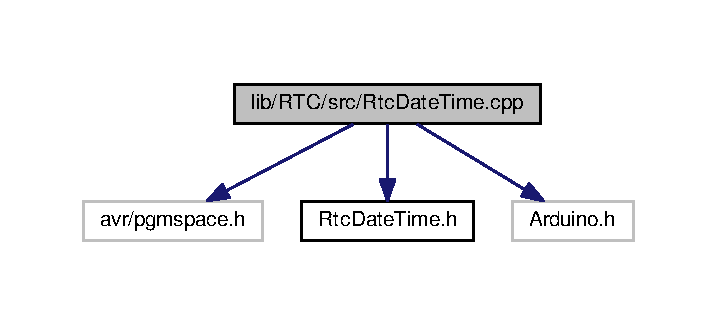
\includegraphics[width=344pt]{_rtc_date_time_8cpp__incl}
\end{center}
\end{figure}
\subsection*{Functions}
\begin{DoxyCompactItemize}
\item 
uint8\+\_\+t \hyperlink{_rtc_date_time_8cpp_a4738b15838d7feb86017668e19d1aa8a}{String\+To\+Uint8} (const char $\ast$p\+String)
\item 
{\footnotesize template$<$typename T $>$ }\\T \hyperlink{_rtc_date_time_8cpp_a854bc39e38fefbf81e0a24409eea91c1}{Days\+Since\+First\+Of\+Year2000} (uint16\+\_\+t year, uint8\+\_\+t month, uint8\+\_\+t day\+Of\+Month)
\item 
{\footnotesize template$<$typename T $>$ }\\T \hyperlink{_rtc_date_time_8cpp_ab1bb7e5421b7179e7509c1df2a34ed5d}{Seconds\+In} (T days, uint8\+\_\+t hours, uint8\+\_\+t minutes, uint8\+\_\+t seconds)
\end{DoxyCompactItemize}
\subsection*{Variables}
\begin{DoxyCompactItemize}
\item 
const uint8\+\_\+t c\+\_\+days\+In\+Month\mbox{[}$\,$\mbox{]} \hyperlink{_rtc_date_time_8cpp_ac0acbe713345b6ba392f37a8f4c8dfb2}{P\+R\+O\+G\+M\+EM} = \{ 31,28,31,30,31,30,31,31,30,31,30,31 \}
\end{DoxyCompactItemize}


\subsection{Function Documentation}
\index{Rtc\+Date\+Time.\+cpp@{Rtc\+Date\+Time.\+cpp}!Days\+Since\+First\+Of\+Year2000@{Days\+Since\+First\+Of\+Year2000}}
\index{Days\+Since\+First\+Of\+Year2000@{Days\+Since\+First\+Of\+Year2000}!Rtc\+Date\+Time.\+cpp@{Rtc\+Date\+Time.\+cpp}}
\subsubsection[{\texorpdfstring{Days\+Since\+First\+Of\+Year2000(uint16\+\_\+t year, uint8\+\_\+t month, uint8\+\_\+t day\+Of\+Month)}{DaysSinceFirstOfYear2000(uint16_t year, uint8_t month, uint8_t dayOfMonth)}}]{\setlength{\rightskip}{0pt plus 5cm}template$<$typename T $>$ T Days\+Since\+First\+Of\+Year2000 (
\begin{DoxyParamCaption}
\item[{uint16\+\_\+t}]{year, }
\item[{uint8\+\_\+t}]{month, }
\item[{uint8\+\_\+t}]{day\+Of\+Month}
\end{DoxyParamCaption}
)}\hypertarget{_rtc_date_time_8cpp_a854bc39e38fefbf81e0a24409eea91c1}{}\label{_rtc_date_time_8cpp_a854bc39e38fefbf81e0a24409eea91c1}


Definition at line 83 of file Rtc\+Date\+Time.\+cpp.

\index{Rtc\+Date\+Time.\+cpp@{Rtc\+Date\+Time.\+cpp}!Seconds\+In@{Seconds\+In}}
\index{Seconds\+In@{Seconds\+In}!Rtc\+Date\+Time.\+cpp@{Rtc\+Date\+Time.\+cpp}}
\subsubsection[{\texorpdfstring{Seconds\+In(\+T days, uint8\+\_\+t hours, uint8\+\_\+t minutes, uint8\+\_\+t seconds)}{SecondsIn(T days, uint8_t hours, uint8_t minutes, uint8_t seconds)}}]{\setlength{\rightskip}{0pt plus 5cm}template$<$typename T $>$ T Seconds\+In (
\begin{DoxyParamCaption}
\item[{T}]{days, }
\item[{uint8\+\_\+t}]{hours, }
\item[{uint8\+\_\+t}]{minutes, }
\item[{uint8\+\_\+t}]{seconds}
\end{DoxyParamCaption}
)}\hypertarget{_rtc_date_time_8cpp_ab1bb7e5421b7179e7509c1df2a34ed5d}{}\label{_rtc_date_time_8cpp_ab1bb7e5421b7179e7509c1df2a34ed5d}


Definition at line 97 of file Rtc\+Date\+Time.\+cpp.

\index{Rtc\+Date\+Time.\+cpp@{Rtc\+Date\+Time.\+cpp}!String\+To\+Uint8@{String\+To\+Uint8}}
\index{String\+To\+Uint8@{String\+To\+Uint8}!Rtc\+Date\+Time.\+cpp@{Rtc\+Date\+Time.\+cpp}}
\subsubsection[{\texorpdfstring{String\+To\+Uint8(const char $\ast$p\+String)}{StringToUint8(const char *pString)}}]{\setlength{\rightskip}{0pt plus 5cm}uint8\+\_\+t String\+To\+Uint8 (
\begin{DoxyParamCaption}
\item[{const char $\ast$}]{p\+String}
\end{DoxyParamCaption}
)}\hypertarget{_rtc_date_time_8cpp_a4738b15838d7feb86017668e19d1aa8a}{}\label{_rtc_date_time_8cpp_a4738b15838d7feb86017668e19d1aa8a}


Definition at line 20 of file Rtc\+Date\+Time.\+cpp.



\subsection{Variable Documentation}
\index{Rtc\+Date\+Time.\+cpp@{Rtc\+Date\+Time.\+cpp}!P\+R\+O\+G\+M\+EM@{P\+R\+O\+G\+M\+EM}}
\index{P\+R\+O\+G\+M\+EM@{P\+R\+O\+G\+M\+EM}!Rtc\+Date\+Time.\+cpp@{Rtc\+Date\+Time.\+cpp}}
\subsubsection[{\texorpdfstring{P\+R\+O\+G\+M\+EM}{PROGMEM}}]{\setlength{\rightskip}{0pt plus 5cm}const uint8\+\_\+t c\+\_\+days\+In\+Month \mbox{[}$\,$\mbox{]} P\+R\+O\+G\+M\+EM = \{ 31,28,31,30,31,30,31,31,30,31,30,31 \}}\hypertarget{_rtc_date_time_8cpp_ac0acbe713345b6ba392f37a8f4c8dfb2}{}\label{_rtc_date_time_8cpp_ac0acbe713345b6ba392f37a8f4c8dfb2}


Definition at line 12 of file Rtc\+Date\+Time.\+cpp.


\hypertarget{_rtc_date_time_8h}{}\section{lib/\+R\+T\+C/src/\+Rtc\+Date\+Time.h File Reference}
\label{_rtc_date_time_8h}\index{lib/\+R\+T\+C/src/\+Rtc\+Date\+Time.\+h@{lib/\+R\+T\+C/src/\+Rtc\+Date\+Time.\+h}}
This graph shows which files directly or indirectly include this file\+:\nopagebreak
\begin{figure}[H]
\begin{center}
\leavevmode
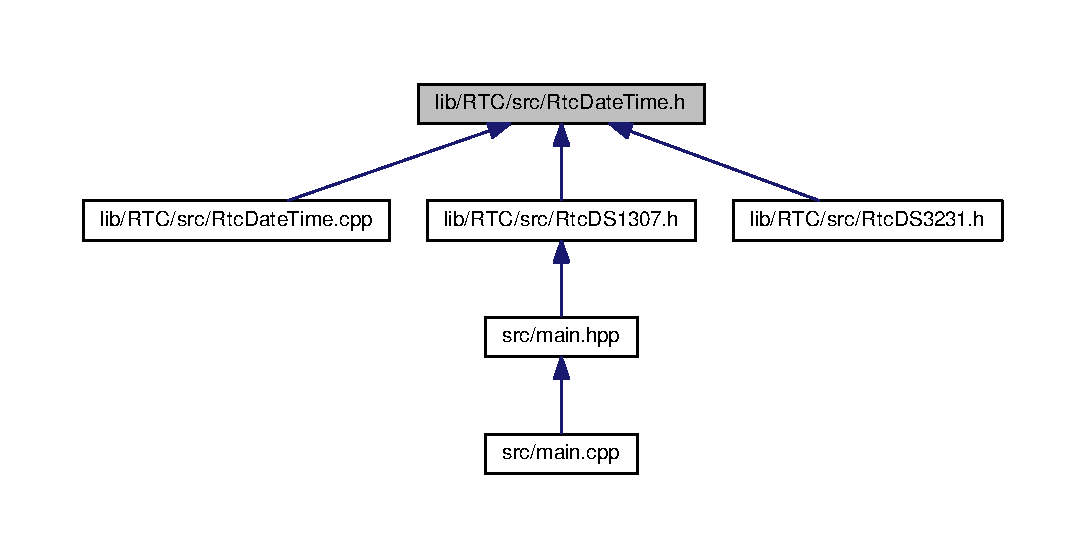
\includegraphics[width=350pt]{_rtc_date_time_8h__dep__incl}
\end{center}
\end{figure}
\subsection*{Classes}
\begin{DoxyCompactItemize}
\item 
class \hyperlink{class_rtc_date_time}{Rtc\+Date\+Time}
\end{DoxyCompactItemize}
\subsection*{Variables}
\begin{DoxyCompactItemize}
\item 
const uint16\+\_\+t \hyperlink{_rtc_date_time_8h_aaf12c47741a61c7d52930cec79b219d9}{c\+\_\+\+Origin\+Year} = 2000
\item 
const uint32\+\_\+t \hyperlink{_rtc_date_time_8h_a18feef96ef5441d842da1cc5bb54462c}{c\+\_\+\+Epoch32\+Of\+Origin\+Year} = 946684800
\item 
const uint8\+\_\+t c\+\_\+days\+In\+Month\mbox{[}$\,$\mbox{]} \hyperlink{_rtc_date_time_8h_ac0acbe713345b6ba392f37a8f4c8dfb2}{P\+R\+O\+G\+M\+EM}
\end{DoxyCompactItemize}


\subsection{Variable Documentation}
\index{Rtc\+Date\+Time.\+h@{Rtc\+Date\+Time.\+h}!c\+\_\+\+Epoch32\+Of\+Origin\+Year@{c\+\_\+\+Epoch32\+Of\+Origin\+Year}}
\index{c\+\_\+\+Epoch32\+Of\+Origin\+Year@{c\+\_\+\+Epoch32\+Of\+Origin\+Year}!Rtc\+Date\+Time.\+h@{Rtc\+Date\+Time.\+h}}
\subsubsection[{\texorpdfstring{c\+\_\+\+Epoch32\+Of\+Origin\+Year}{c_Epoch32OfOriginYear}}]{\setlength{\rightskip}{0pt plus 5cm}const uint32\+\_\+t c\+\_\+\+Epoch32\+Of\+Origin\+Year = 946684800}\hypertarget{_rtc_date_time_8h_a18feef96ef5441d842da1cc5bb54462c}{}\label{_rtc_date_time_8h_a18feef96ef5441d842da1cc5bb54462c}


Definition at line 7 of file Rtc\+Date\+Time.\+h.

\index{Rtc\+Date\+Time.\+h@{Rtc\+Date\+Time.\+h}!c\+\_\+\+Origin\+Year@{c\+\_\+\+Origin\+Year}}
\index{c\+\_\+\+Origin\+Year@{c\+\_\+\+Origin\+Year}!Rtc\+Date\+Time.\+h@{Rtc\+Date\+Time.\+h}}
\subsubsection[{\texorpdfstring{c\+\_\+\+Origin\+Year}{c_OriginYear}}]{\setlength{\rightskip}{0pt plus 5cm}const uint16\+\_\+t c\+\_\+\+Origin\+Year = 2000}\hypertarget{_rtc_date_time_8h_aaf12c47741a61c7d52930cec79b219d9}{}\label{_rtc_date_time_8h_aaf12c47741a61c7d52930cec79b219d9}


Definition at line 6 of file Rtc\+Date\+Time.\+h.

\index{Rtc\+Date\+Time.\+h@{Rtc\+Date\+Time.\+h}!P\+R\+O\+G\+M\+EM@{P\+R\+O\+G\+M\+EM}}
\index{P\+R\+O\+G\+M\+EM@{P\+R\+O\+G\+M\+EM}!Rtc\+Date\+Time.\+h@{Rtc\+Date\+Time.\+h}}
\subsubsection[{\texorpdfstring{P\+R\+O\+G\+M\+EM}{PROGMEM}}]{\setlength{\rightskip}{0pt plus 5cm}const uint8\+\_\+t c\+\_\+days\+In\+Month \mbox{[}$\,$\mbox{]} P\+R\+O\+G\+M\+EM}\hypertarget{_rtc_date_time_8h_ac0acbe713345b6ba392f37a8f4c8dfb2}{}\label{_rtc_date_time_8h_ac0acbe713345b6ba392f37a8f4c8dfb2}


Definition at line 12 of file Rtc\+Date\+Time.\+cpp.


\hypertarget{_rtc_d_s1307_8h}{}\section{lib/\+R\+T\+C/src/\+Rtc\+D\+S1307.h File Reference}
\label{_rtc_d_s1307_8h}\index{lib/\+R\+T\+C/src/\+Rtc\+D\+S1307.\+h@{lib/\+R\+T\+C/src/\+Rtc\+D\+S1307.\+h}}
{\ttfamily \#include $<$Arduino.\+h$>$}\\*
{\ttfamily \#include $<$Rtc\+Date\+Time.\+h$>$}\\*
{\ttfamily \#include \char`\"{}Rtc\+Utility.\+h\char`\"{}}\\*
Include dependency graph for Rtc\+D\+S1307.\+h\+:\nopagebreak
\begin{figure}[H]
\begin{center}
\leavevmode
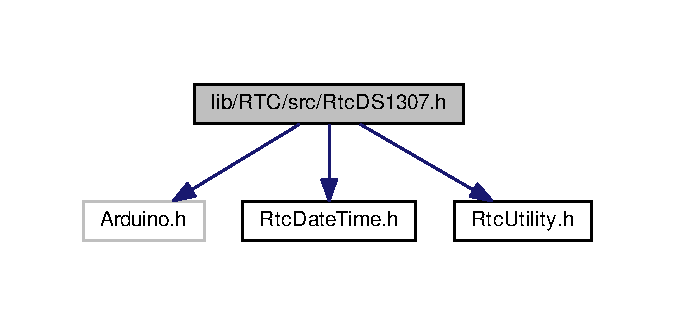
\includegraphics[width=324pt]{_rtc_d_s1307_8h__incl}
\end{center}
\end{figure}
This graph shows which files directly or indirectly include this file\+:\nopagebreak
\begin{figure}[H]
\begin{center}
\leavevmode
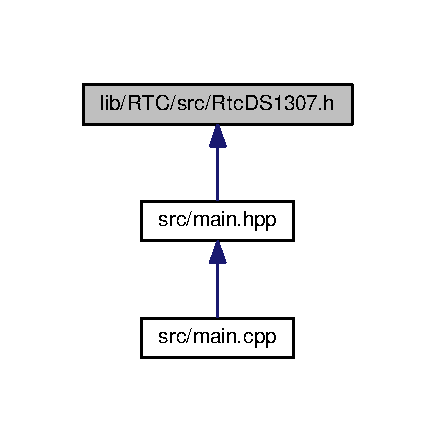
\includegraphics[width=209pt]{_rtc_d_s1307_8h__dep__incl}
\end{center}
\end{figure}
\subsection*{Classes}
\begin{DoxyCompactItemize}
\item 
class \hyperlink{class_rtc_d_s1307}{Rtc\+D\+S1307$<$ T\+\_\+\+W\+I\+R\+E\+\_\+\+M\+E\+T\+H\+O\+D $>$}
\end{DoxyCompactItemize}
\subsection*{Enumerations}
\begin{DoxyCompactItemize}
\item 
enum \hyperlink{_rtc_d_s1307_8h_a85910be6fed3842f050e1e3e3c03f229}{D\+S1307\+Square\+Wave\+Out} \{ \\*
\hyperlink{_rtc_d_s1307_8h_a85910be6fed3842f050e1e3e3c03f229af0e58bf3703c39c0786c4a6cb3d3b47d}{D\+S1307\+Square\+Wave\+Out\+\_\+1\+Hz} = 0b00010000, 
\hyperlink{_rtc_d_s1307_8h_a85910be6fed3842f050e1e3e3c03f229acc32b1350cf51a76f7f1d55977ee84e0}{D\+S1307\+Square\+Wave\+Out\+\_\+4k\+Hz} = 0b00010001, 
\hyperlink{_rtc_d_s1307_8h_a85910be6fed3842f050e1e3e3c03f229ae79b3ba265c8ed7d326620aacaaf719d}{D\+S1307\+Square\+Wave\+Out\+\_\+8k\+Hz} = 0b00010010, 
\hyperlink{_rtc_d_s1307_8h_a85910be6fed3842f050e1e3e3c03f229a68aecd02fa77fe51d090425485f83359}{D\+S1307\+Square\+Wave\+Out\+\_\+32k\+Hz} = 0b00010011, 
\\*
\hyperlink{_rtc_d_s1307_8h_a85910be6fed3842f050e1e3e3c03f229a906bb03aebf2667c8db8d55cae850d4e}{D\+S1307\+Square\+Wave\+Out\+\_\+\+High} = 0b10000000, 
\hyperlink{_rtc_d_s1307_8h_a85910be6fed3842f050e1e3e3c03f229adb48767edb56cde82e1375eeeed93dd0}{D\+S1307\+Square\+Wave\+Out\+\_\+\+Low} = 0b00000000
 \}
\end{DoxyCompactItemize}
\subsection*{Variables}
\begin{DoxyCompactItemize}
\item 
const uint8\+\_\+t \hyperlink{_rtc_d_s1307_8h_af2c547a2efa8e3c09d8eca2ad1eba7fb}{D\+S1307\+\_\+\+A\+D\+D\+R\+E\+SS} = 0x68
\item 
const uint8\+\_\+t \hyperlink{_rtc_d_s1307_8h_a9916cb27639f2ac147e7567fae6fc2d6}{D\+S1307\+\_\+\+R\+E\+G\+\_\+\+T\+I\+M\+E\+D\+A\+TE} = 0x00
\item 
const uint8\+\_\+t \hyperlink{_rtc_d_s1307_8h_aa5fa515847c7cf48fc32085b3c52f5b2}{D\+S1307\+\_\+\+R\+E\+G\+\_\+\+S\+T\+A\+T\+US} = 0x00
\item 
const uint8\+\_\+t \hyperlink{_rtc_d_s1307_8h_a56374477c784fc831fc5b3012e5ce974}{D\+S1307\+\_\+\+R\+E\+G\+\_\+\+C\+O\+N\+T\+R\+OL} = 0x07
\item 
const uint8\+\_\+t \hyperlink{_rtc_d_s1307_8h_a5722fbbb40faed3fa6026c3496756c74}{D\+S1307\+\_\+\+R\+E\+G\+\_\+\+R\+A\+M\+S\+T\+A\+RT} = 0x08
\item 
const uint8\+\_\+t \hyperlink{_rtc_d_s1307_8h_a005ab13e399c5369cfb5bfc1e466ea6f}{D\+S1307\+\_\+\+R\+E\+G\+\_\+\+R\+A\+M\+E\+ND} = 0x3f
\item 
const uint8\+\_\+t \hyperlink{_rtc_d_s1307_8h_afbc088ffc39b051bcb17cef8063f92f2}{D\+S1307\+\_\+\+R\+E\+G\+\_\+\+R\+A\+M\+S\+I\+ZE} = \hyperlink{_rtc_d_s1307_8h_a005ab13e399c5369cfb5bfc1e466ea6f}{D\+S1307\+\_\+\+R\+E\+G\+\_\+\+R\+A\+M\+E\+ND} -\/ \hyperlink{_rtc_d_s1307_8h_a5722fbbb40faed3fa6026c3496756c74}{D\+S1307\+\_\+\+R\+E\+G\+\_\+\+R\+A\+M\+S\+T\+A\+RT}
\item 
const uint8\+\_\+t \hyperlink{_rtc_d_s1307_8h_a5b8cb614123fc430bb2e33f60b07ee4f}{D\+S1307\+\_\+\+R\+E\+G\+\_\+\+T\+I\+M\+E\+D\+A\+T\+E\+\_\+\+S\+I\+ZE} = 7
\item 
const uint8\+\_\+t \hyperlink{_rtc_d_s1307_8h_a9c2106d1de67e1c3f0c6da157b747b8d}{D\+S1307\+\_\+\+R\+S0} = 0
\item 
const uint8\+\_\+t \hyperlink{_rtc_d_s1307_8h_ad6a2a38a19cb0d93569bb73d348416a4}{D\+S1307\+\_\+\+R\+S1} = 1
\item 
const uint8\+\_\+t \hyperlink{_rtc_d_s1307_8h_a2e35028ae919bb33c5036cffe02e210f}{D\+S1307\+\_\+\+S\+Q\+WE} = 4
\item 
const uint8\+\_\+t \hyperlink{_rtc_d_s1307_8h_a335feee443ff3180194fbaf19cf34364}{D\+S1307\+\_\+\+O\+UT} = 7
\item 
const uint8\+\_\+t \hyperlink{_rtc_d_s1307_8h_a057f35cec5e217c7ac7a9aadfaf473ff}{D\+S1307\+\_\+\+CH} = 7
\end{DoxyCompactItemize}


\subsection{Enumeration Type Documentation}
\index{Rtc\+D\+S1307.\+h@{Rtc\+D\+S1307.\+h}!D\+S1307\+Square\+Wave\+Out@{D\+S1307\+Square\+Wave\+Out}}
\index{D\+S1307\+Square\+Wave\+Out@{D\+S1307\+Square\+Wave\+Out}!Rtc\+D\+S1307.\+h@{Rtc\+D\+S1307.\+h}}
\subsubsection[{\texorpdfstring{D\+S1307\+Square\+Wave\+Out}{DS1307SquareWaveOut}}]{\setlength{\rightskip}{0pt plus 5cm}enum {\bf D\+S1307\+Square\+Wave\+Out}}\hypertarget{_rtc_d_s1307_8h_a85910be6fed3842f050e1e3e3c03f229}{}\label{_rtc_d_s1307_8h_a85910be6fed3842f050e1e3e3c03f229}
\begin{Desc}
\item[Enumerator]\par
\begin{description}
\index{D\+S1307\+Square\+Wave\+Out\+\_\+1\+Hz@{D\+S1307\+Square\+Wave\+Out\+\_\+1\+Hz}!Rtc\+D\+S1307.\+h@{Rtc\+D\+S1307.\+h}}\index{Rtc\+D\+S1307.\+h@{Rtc\+D\+S1307.\+h}!D\+S1307\+Square\+Wave\+Out\+\_\+1\+Hz@{D\+S1307\+Square\+Wave\+Out\+\_\+1\+Hz}}\item[{\em 
D\+S1307\+Square\+Wave\+Out\+\_\+1\+Hz\hypertarget{_rtc_d_s1307_8h_a85910be6fed3842f050e1e3e3c03f229af0e58bf3703c39c0786c4a6cb3d3b47d}{}\label{_rtc_d_s1307_8h_a85910be6fed3842f050e1e3e3c03f229af0e58bf3703c39c0786c4a6cb3d3b47d}
}]\index{D\+S1307\+Square\+Wave\+Out\+\_\+4k\+Hz@{D\+S1307\+Square\+Wave\+Out\+\_\+4k\+Hz}!Rtc\+D\+S1307.\+h@{Rtc\+D\+S1307.\+h}}\index{Rtc\+D\+S1307.\+h@{Rtc\+D\+S1307.\+h}!D\+S1307\+Square\+Wave\+Out\+\_\+4k\+Hz@{D\+S1307\+Square\+Wave\+Out\+\_\+4k\+Hz}}\item[{\em 
D\+S1307\+Square\+Wave\+Out\+\_\+4k\+Hz\hypertarget{_rtc_d_s1307_8h_a85910be6fed3842f050e1e3e3c03f229acc32b1350cf51a76f7f1d55977ee84e0}{}\label{_rtc_d_s1307_8h_a85910be6fed3842f050e1e3e3c03f229acc32b1350cf51a76f7f1d55977ee84e0}
}]\index{D\+S1307\+Square\+Wave\+Out\+\_\+8k\+Hz@{D\+S1307\+Square\+Wave\+Out\+\_\+8k\+Hz}!Rtc\+D\+S1307.\+h@{Rtc\+D\+S1307.\+h}}\index{Rtc\+D\+S1307.\+h@{Rtc\+D\+S1307.\+h}!D\+S1307\+Square\+Wave\+Out\+\_\+8k\+Hz@{D\+S1307\+Square\+Wave\+Out\+\_\+8k\+Hz}}\item[{\em 
D\+S1307\+Square\+Wave\+Out\+\_\+8k\+Hz\hypertarget{_rtc_d_s1307_8h_a85910be6fed3842f050e1e3e3c03f229ae79b3ba265c8ed7d326620aacaaf719d}{}\label{_rtc_d_s1307_8h_a85910be6fed3842f050e1e3e3c03f229ae79b3ba265c8ed7d326620aacaaf719d}
}]\index{D\+S1307\+Square\+Wave\+Out\+\_\+32k\+Hz@{D\+S1307\+Square\+Wave\+Out\+\_\+32k\+Hz}!Rtc\+D\+S1307.\+h@{Rtc\+D\+S1307.\+h}}\index{Rtc\+D\+S1307.\+h@{Rtc\+D\+S1307.\+h}!D\+S1307\+Square\+Wave\+Out\+\_\+32k\+Hz@{D\+S1307\+Square\+Wave\+Out\+\_\+32k\+Hz}}\item[{\em 
D\+S1307\+Square\+Wave\+Out\+\_\+32k\+Hz\hypertarget{_rtc_d_s1307_8h_a85910be6fed3842f050e1e3e3c03f229a68aecd02fa77fe51d090425485f83359}{}\label{_rtc_d_s1307_8h_a85910be6fed3842f050e1e3e3c03f229a68aecd02fa77fe51d090425485f83359}
}]\index{D\+S1307\+Square\+Wave\+Out\+\_\+\+High@{D\+S1307\+Square\+Wave\+Out\+\_\+\+High}!Rtc\+D\+S1307.\+h@{Rtc\+D\+S1307.\+h}}\index{Rtc\+D\+S1307.\+h@{Rtc\+D\+S1307.\+h}!D\+S1307\+Square\+Wave\+Out\+\_\+\+High@{D\+S1307\+Square\+Wave\+Out\+\_\+\+High}}\item[{\em 
D\+S1307\+Square\+Wave\+Out\+\_\+\+High\hypertarget{_rtc_d_s1307_8h_a85910be6fed3842f050e1e3e3c03f229a906bb03aebf2667c8db8d55cae850d4e}{}\label{_rtc_d_s1307_8h_a85910be6fed3842f050e1e3e3c03f229a906bb03aebf2667c8db8d55cae850d4e}
}]\index{D\+S1307\+Square\+Wave\+Out\+\_\+\+Low@{D\+S1307\+Square\+Wave\+Out\+\_\+\+Low}!Rtc\+D\+S1307.\+h@{Rtc\+D\+S1307.\+h}}\index{Rtc\+D\+S1307.\+h@{Rtc\+D\+S1307.\+h}!D\+S1307\+Square\+Wave\+Out\+\_\+\+Low@{D\+S1307\+Square\+Wave\+Out\+\_\+\+Low}}\item[{\em 
D\+S1307\+Square\+Wave\+Out\+\_\+\+Low\hypertarget{_rtc_d_s1307_8h_a85910be6fed3842f050e1e3e3c03f229adb48767edb56cde82e1375eeeed93dd0}{}\label{_rtc_d_s1307_8h_a85910be6fed3842f050e1e3e3c03f229adb48767edb56cde82e1375eeeed93dd0}
}]\end{description}
\end{Desc}


Definition at line 33 of file Rtc\+D\+S1307.\+h.



\subsection{Variable Documentation}
\index{Rtc\+D\+S1307.\+h@{Rtc\+D\+S1307.\+h}!D\+S1307\+\_\+\+A\+D\+D\+R\+E\+SS@{D\+S1307\+\_\+\+A\+D\+D\+R\+E\+SS}}
\index{D\+S1307\+\_\+\+A\+D\+D\+R\+E\+SS@{D\+S1307\+\_\+\+A\+D\+D\+R\+E\+SS}!Rtc\+D\+S1307.\+h@{Rtc\+D\+S1307.\+h}}
\subsubsection[{\texorpdfstring{D\+S1307\+\_\+\+A\+D\+D\+R\+E\+SS}{DS1307_ADDRESS}}]{\setlength{\rightskip}{0pt plus 5cm}const uint8\+\_\+t D\+S1307\+\_\+\+A\+D\+D\+R\+E\+SS = 0x68}\hypertarget{_rtc_d_s1307_8h_af2c547a2efa8e3c09d8eca2ad1eba7fb}{}\label{_rtc_d_s1307_8h_af2c547a2efa8e3c09d8eca2ad1eba7fb}


Definition at line 11 of file Rtc\+D\+S1307.\+h.

\index{Rtc\+D\+S1307.\+h@{Rtc\+D\+S1307.\+h}!D\+S1307\+\_\+\+CH@{D\+S1307\+\_\+\+CH}}
\index{D\+S1307\+\_\+\+CH@{D\+S1307\+\_\+\+CH}!Rtc\+D\+S1307.\+h@{Rtc\+D\+S1307.\+h}}
\subsubsection[{\texorpdfstring{D\+S1307\+\_\+\+CH}{DS1307_CH}}]{\setlength{\rightskip}{0pt plus 5cm}const uint8\+\_\+t D\+S1307\+\_\+\+CH = 7}\hypertarget{_rtc_d_s1307_8h_a057f35cec5e217c7ac7a9aadfaf473ff}{}\label{_rtc_d_s1307_8h_a057f35cec5e217c7ac7a9aadfaf473ff}


Definition at line 31 of file Rtc\+D\+S1307.\+h.

\index{Rtc\+D\+S1307.\+h@{Rtc\+D\+S1307.\+h}!D\+S1307\+\_\+\+O\+UT@{D\+S1307\+\_\+\+O\+UT}}
\index{D\+S1307\+\_\+\+O\+UT@{D\+S1307\+\_\+\+O\+UT}!Rtc\+D\+S1307.\+h@{Rtc\+D\+S1307.\+h}}
\subsubsection[{\texorpdfstring{D\+S1307\+\_\+\+O\+UT}{DS1307_OUT}}]{\setlength{\rightskip}{0pt plus 5cm}const uint8\+\_\+t D\+S1307\+\_\+\+O\+UT = 7}\hypertarget{_rtc_d_s1307_8h_a335feee443ff3180194fbaf19cf34364}{}\label{_rtc_d_s1307_8h_a335feee443ff3180194fbaf19cf34364}


Definition at line 28 of file Rtc\+D\+S1307.\+h.

\index{Rtc\+D\+S1307.\+h@{Rtc\+D\+S1307.\+h}!D\+S1307\+\_\+\+R\+E\+G\+\_\+\+C\+O\+N\+T\+R\+OL@{D\+S1307\+\_\+\+R\+E\+G\+\_\+\+C\+O\+N\+T\+R\+OL}}
\index{D\+S1307\+\_\+\+R\+E\+G\+\_\+\+C\+O\+N\+T\+R\+OL@{D\+S1307\+\_\+\+R\+E\+G\+\_\+\+C\+O\+N\+T\+R\+OL}!Rtc\+D\+S1307.\+h@{Rtc\+D\+S1307.\+h}}
\subsubsection[{\texorpdfstring{D\+S1307\+\_\+\+R\+E\+G\+\_\+\+C\+O\+N\+T\+R\+OL}{DS1307_REG_CONTROL}}]{\setlength{\rightskip}{0pt plus 5cm}const uint8\+\_\+t D\+S1307\+\_\+\+R\+E\+G\+\_\+\+C\+O\+N\+T\+R\+OL = 0x07}\hypertarget{_rtc_d_s1307_8h_a56374477c784fc831fc5b3012e5ce974}{}\label{_rtc_d_s1307_8h_a56374477c784fc831fc5b3012e5ce974}


Definition at line 16 of file Rtc\+D\+S1307.\+h.

\index{Rtc\+D\+S1307.\+h@{Rtc\+D\+S1307.\+h}!D\+S1307\+\_\+\+R\+E\+G\+\_\+\+R\+A\+M\+E\+ND@{D\+S1307\+\_\+\+R\+E\+G\+\_\+\+R\+A\+M\+E\+ND}}
\index{D\+S1307\+\_\+\+R\+E\+G\+\_\+\+R\+A\+M\+E\+ND@{D\+S1307\+\_\+\+R\+E\+G\+\_\+\+R\+A\+M\+E\+ND}!Rtc\+D\+S1307.\+h@{Rtc\+D\+S1307.\+h}}
\subsubsection[{\texorpdfstring{D\+S1307\+\_\+\+R\+E\+G\+\_\+\+R\+A\+M\+E\+ND}{DS1307_REG_RAMEND}}]{\setlength{\rightskip}{0pt plus 5cm}const uint8\+\_\+t D\+S1307\+\_\+\+R\+E\+G\+\_\+\+R\+A\+M\+E\+ND = 0x3f}\hypertarget{_rtc_d_s1307_8h_a005ab13e399c5369cfb5bfc1e466ea6f}{}\label{_rtc_d_s1307_8h_a005ab13e399c5369cfb5bfc1e466ea6f}


Definition at line 18 of file Rtc\+D\+S1307.\+h.

\index{Rtc\+D\+S1307.\+h@{Rtc\+D\+S1307.\+h}!D\+S1307\+\_\+\+R\+E\+G\+\_\+\+R\+A\+M\+S\+I\+ZE@{D\+S1307\+\_\+\+R\+E\+G\+\_\+\+R\+A\+M\+S\+I\+ZE}}
\index{D\+S1307\+\_\+\+R\+E\+G\+\_\+\+R\+A\+M\+S\+I\+ZE@{D\+S1307\+\_\+\+R\+E\+G\+\_\+\+R\+A\+M\+S\+I\+ZE}!Rtc\+D\+S1307.\+h@{Rtc\+D\+S1307.\+h}}
\subsubsection[{\texorpdfstring{D\+S1307\+\_\+\+R\+E\+G\+\_\+\+R\+A\+M\+S\+I\+ZE}{DS1307_REG_RAMSIZE}}]{\setlength{\rightskip}{0pt plus 5cm}const uint8\+\_\+t D\+S1307\+\_\+\+R\+E\+G\+\_\+\+R\+A\+M\+S\+I\+ZE = {\bf D\+S1307\+\_\+\+R\+E\+G\+\_\+\+R\+A\+M\+E\+ND} -\/ {\bf D\+S1307\+\_\+\+R\+E\+G\+\_\+\+R\+A\+M\+S\+T\+A\+RT}}\hypertarget{_rtc_d_s1307_8h_afbc088ffc39b051bcb17cef8063f92f2}{}\label{_rtc_d_s1307_8h_afbc088ffc39b051bcb17cef8063f92f2}


Definition at line 19 of file Rtc\+D\+S1307.\+h.

\index{Rtc\+D\+S1307.\+h@{Rtc\+D\+S1307.\+h}!D\+S1307\+\_\+\+R\+E\+G\+\_\+\+R\+A\+M\+S\+T\+A\+RT@{D\+S1307\+\_\+\+R\+E\+G\+\_\+\+R\+A\+M\+S\+T\+A\+RT}}
\index{D\+S1307\+\_\+\+R\+E\+G\+\_\+\+R\+A\+M\+S\+T\+A\+RT@{D\+S1307\+\_\+\+R\+E\+G\+\_\+\+R\+A\+M\+S\+T\+A\+RT}!Rtc\+D\+S1307.\+h@{Rtc\+D\+S1307.\+h}}
\subsubsection[{\texorpdfstring{D\+S1307\+\_\+\+R\+E\+G\+\_\+\+R\+A\+M\+S\+T\+A\+RT}{DS1307_REG_RAMSTART}}]{\setlength{\rightskip}{0pt plus 5cm}const uint8\+\_\+t D\+S1307\+\_\+\+R\+E\+G\+\_\+\+R\+A\+M\+S\+T\+A\+RT = 0x08}\hypertarget{_rtc_d_s1307_8h_a5722fbbb40faed3fa6026c3496756c74}{}\label{_rtc_d_s1307_8h_a5722fbbb40faed3fa6026c3496756c74}


Definition at line 17 of file Rtc\+D\+S1307.\+h.

\index{Rtc\+D\+S1307.\+h@{Rtc\+D\+S1307.\+h}!D\+S1307\+\_\+\+R\+E\+G\+\_\+\+S\+T\+A\+T\+US@{D\+S1307\+\_\+\+R\+E\+G\+\_\+\+S\+T\+A\+T\+US}}
\index{D\+S1307\+\_\+\+R\+E\+G\+\_\+\+S\+T\+A\+T\+US@{D\+S1307\+\_\+\+R\+E\+G\+\_\+\+S\+T\+A\+T\+US}!Rtc\+D\+S1307.\+h@{Rtc\+D\+S1307.\+h}}
\subsubsection[{\texorpdfstring{D\+S1307\+\_\+\+R\+E\+G\+\_\+\+S\+T\+A\+T\+US}{DS1307_REG_STATUS}}]{\setlength{\rightskip}{0pt plus 5cm}const uint8\+\_\+t D\+S1307\+\_\+\+R\+E\+G\+\_\+\+S\+T\+A\+T\+US = 0x00}\hypertarget{_rtc_d_s1307_8h_aa5fa515847c7cf48fc32085b3c52f5b2}{}\label{_rtc_d_s1307_8h_aa5fa515847c7cf48fc32085b3c52f5b2}


Definition at line 15 of file Rtc\+D\+S1307.\+h.

\index{Rtc\+D\+S1307.\+h@{Rtc\+D\+S1307.\+h}!D\+S1307\+\_\+\+R\+E\+G\+\_\+\+T\+I\+M\+E\+D\+A\+TE@{D\+S1307\+\_\+\+R\+E\+G\+\_\+\+T\+I\+M\+E\+D\+A\+TE}}
\index{D\+S1307\+\_\+\+R\+E\+G\+\_\+\+T\+I\+M\+E\+D\+A\+TE@{D\+S1307\+\_\+\+R\+E\+G\+\_\+\+T\+I\+M\+E\+D\+A\+TE}!Rtc\+D\+S1307.\+h@{Rtc\+D\+S1307.\+h}}
\subsubsection[{\texorpdfstring{D\+S1307\+\_\+\+R\+E\+G\+\_\+\+T\+I\+M\+E\+D\+A\+TE}{DS1307_REG_TIMEDATE}}]{\setlength{\rightskip}{0pt plus 5cm}const uint8\+\_\+t D\+S1307\+\_\+\+R\+E\+G\+\_\+\+T\+I\+M\+E\+D\+A\+TE = 0x00}\hypertarget{_rtc_d_s1307_8h_a9916cb27639f2ac147e7567fae6fc2d6}{}\label{_rtc_d_s1307_8h_a9916cb27639f2ac147e7567fae6fc2d6}


Definition at line 14 of file Rtc\+D\+S1307.\+h.

\index{Rtc\+D\+S1307.\+h@{Rtc\+D\+S1307.\+h}!D\+S1307\+\_\+\+R\+E\+G\+\_\+\+T\+I\+M\+E\+D\+A\+T\+E\+\_\+\+S\+I\+ZE@{D\+S1307\+\_\+\+R\+E\+G\+\_\+\+T\+I\+M\+E\+D\+A\+T\+E\+\_\+\+S\+I\+ZE}}
\index{D\+S1307\+\_\+\+R\+E\+G\+\_\+\+T\+I\+M\+E\+D\+A\+T\+E\+\_\+\+S\+I\+ZE@{D\+S1307\+\_\+\+R\+E\+G\+\_\+\+T\+I\+M\+E\+D\+A\+T\+E\+\_\+\+S\+I\+ZE}!Rtc\+D\+S1307.\+h@{Rtc\+D\+S1307.\+h}}
\subsubsection[{\texorpdfstring{D\+S1307\+\_\+\+R\+E\+G\+\_\+\+T\+I\+M\+E\+D\+A\+T\+E\+\_\+\+S\+I\+ZE}{DS1307_REG_TIMEDATE_SIZE}}]{\setlength{\rightskip}{0pt plus 5cm}const uint8\+\_\+t D\+S1307\+\_\+\+R\+E\+G\+\_\+\+T\+I\+M\+E\+D\+A\+T\+E\+\_\+\+S\+I\+ZE = 7}\hypertarget{_rtc_d_s1307_8h_a5b8cb614123fc430bb2e33f60b07ee4f}{}\label{_rtc_d_s1307_8h_a5b8cb614123fc430bb2e33f60b07ee4f}


Definition at line 22 of file Rtc\+D\+S1307.\+h.

\index{Rtc\+D\+S1307.\+h@{Rtc\+D\+S1307.\+h}!D\+S1307\+\_\+\+R\+S0@{D\+S1307\+\_\+\+R\+S0}}
\index{D\+S1307\+\_\+\+R\+S0@{D\+S1307\+\_\+\+R\+S0}!Rtc\+D\+S1307.\+h@{Rtc\+D\+S1307.\+h}}
\subsubsection[{\texorpdfstring{D\+S1307\+\_\+\+R\+S0}{DS1307_RS0}}]{\setlength{\rightskip}{0pt plus 5cm}const uint8\+\_\+t D\+S1307\+\_\+\+R\+S0 = 0}\hypertarget{_rtc_d_s1307_8h_a9c2106d1de67e1c3f0c6da157b747b8d}{}\label{_rtc_d_s1307_8h_a9c2106d1de67e1c3f0c6da157b747b8d}


Definition at line 25 of file Rtc\+D\+S1307.\+h.

\index{Rtc\+D\+S1307.\+h@{Rtc\+D\+S1307.\+h}!D\+S1307\+\_\+\+R\+S1@{D\+S1307\+\_\+\+R\+S1}}
\index{D\+S1307\+\_\+\+R\+S1@{D\+S1307\+\_\+\+R\+S1}!Rtc\+D\+S1307.\+h@{Rtc\+D\+S1307.\+h}}
\subsubsection[{\texorpdfstring{D\+S1307\+\_\+\+R\+S1}{DS1307_RS1}}]{\setlength{\rightskip}{0pt plus 5cm}const uint8\+\_\+t D\+S1307\+\_\+\+R\+S1 = 1}\hypertarget{_rtc_d_s1307_8h_ad6a2a38a19cb0d93569bb73d348416a4}{}\label{_rtc_d_s1307_8h_ad6a2a38a19cb0d93569bb73d348416a4}


Definition at line 26 of file Rtc\+D\+S1307.\+h.

\index{Rtc\+D\+S1307.\+h@{Rtc\+D\+S1307.\+h}!D\+S1307\+\_\+\+S\+Q\+WE@{D\+S1307\+\_\+\+S\+Q\+WE}}
\index{D\+S1307\+\_\+\+S\+Q\+WE@{D\+S1307\+\_\+\+S\+Q\+WE}!Rtc\+D\+S1307.\+h@{Rtc\+D\+S1307.\+h}}
\subsubsection[{\texorpdfstring{D\+S1307\+\_\+\+S\+Q\+WE}{DS1307_SQWE}}]{\setlength{\rightskip}{0pt plus 5cm}const uint8\+\_\+t D\+S1307\+\_\+\+S\+Q\+WE = 4}\hypertarget{_rtc_d_s1307_8h_a2e35028ae919bb33c5036cffe02e210f}{}\label{_rtc_d_s1307_8h_a2e35028ae919bb33c5036cffe02e210f}


Definition at line 27 of file Rtc\+D\+S1307.\+h.


\hypertarget{_rtc_d_s3231_8h}{}\section{lib/\+R\+T\+C/src/\+Rtc\+D\+S3231.h File Reference}
\label{_rtc_d_s3231_8h}\index{lib/\+R\+T\+C/src/\+Rtc\+D\+S3231.\+h@{lib/\+R\+T\+C/src/\+Rtc\+D\+S3231.\+h}}
{\ttfamily \#include $<$Arduino.\+h$>$}\\*
{\ttfamily \#include $<$Rtc\+Date\+Time.\+h$>$}\\*
{\ttfamily \#include $<$Rtc\+Temperature.\+h$>$}\\*
{\ttfamily \#include \char`\"{}Rtc\+Utility.\+h\char`\"{}}\\*
Include dependency graph for Rtc\+D\+S3231.\+h\+:\nopagebreak
\begin{figure}[H]
\begin{center}
\leavevmode
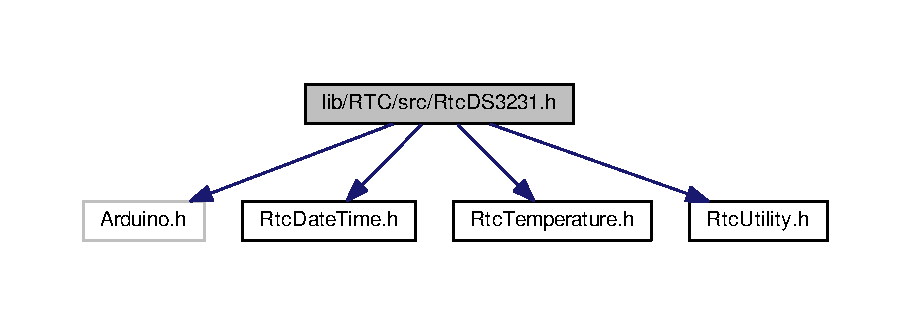
\includegraphics[width=350pt]{_rtc_d_s3231_8h__incl}
\end{center}
\end{figure}
\subsection*{Classes}
\begin{DoxyCompactItemize}
\item 
class \hyperlink{class_d_s3231_alarm_one}{D\+S3231\+Alarm\+One}
\item 
class \hyperlink{class_d_s3231_alarm_two}{D\+S3231\+Alarm\+Two}
\item 
class \hyperlink{class_rtc_d_s3231}{Rtc\+D\+S3231$<$ T\+\_\+\+W\+I\+R\+E\+\_\+\+M\+E\+T\+H\+O\+D $>$}
\end{DoxyCompactItemize}
\subsection*{Enumerations}
\begin{DoxyCompactItemize}
\item 
enum \hyperlink{_rtc_d_s3231_8h_aee303344b910c99a596a83018642f2a7}{D\+S3231\+Alarm\+One\+Control} \{ \\*
\hyperlink{_rtc_d_s3231_8h_aee303344b910c99a596a83018642f2a7a64bc953a8218ce9b030f0270512dbaa2}{D\+S3231\+Alarm\+One\+Control\+\_\+\+Hours\+Minutes\+Seconds\+Day\+Of\+Month\+Match} = 0x00, 
\hyperlink{_rtc_d_s3231_8h_aee303344b910c99a596a83018642f2a7a9ab9f73b2657f0acddb2052ca635f071}{D\+S3231\+Alarm\+One\+Control\+\_\+\+Once\+Per\+Second} = 0x17, 
\hyperlink{_rtc_d_s3231_8h_aee303344b910c99a596a83018642f2a7ad2ba9b378411bdd13d217e626fa35dcf}{D\+S3231\+Alarm\+One\+Control\+\_\+\+Seconds\+Match} = 0x16, 
\hyperlink{_rtc_d_s3231_8h_aee303344b910c99a596a83018642f2a7aa3d896284536561a11c535c608006acf}{D\+S3231\+Alarm\+One\+Control\+\_\+\+Minutes\+Seconds\+Match} = 0x14, 
\\*
\hyperlink{_rtc_d_s3231_8h_aee303344b910c99a596a83018642f2a7a04c375ddcdcca38eb56a8b8812057340}{D\+S3231\+Alarm\+One\+Control\+\_\+\+Hours\+Minutes\+Seconds\+Match} = 0x10, 
\hyperlink{_rtc_d_s3231_8h_aee303344b910c99a596a83018642f2a7a55560520bf190342d1d17c4999b2b7c2}{D\+S3231\+Alarm\+One\+Control\+\_\+\+Hours\+Minutes\+Seconds\+Day\+Of\+Week\+Match} = 0x08
 \}
\item 
enum \hyperlink{_rtc_d_s3231_8h_a453a5caa2fec7d65bbc41f1b3e93a8ea}{D\+S3231\+Alarm\+Two\+Control} \{ \\*
\hyperlink{_rtc_d_s3231_8h_a453a5caa2fec7d65bbc41f1b3e93a8eaaad1ae7dacbfa21b7db1efd733fa7d7f9}{D\+S3231\+Alarm\+Two\+Control\+\_\+\+Hours\+Minutes\+Day\+Of\+Month\+Match} = 0x00, 
\hyperlink{_rtc_d_s3231_8h_a453a5caa2fec7d65bbc41f1b3e93a8eaa36d1e29b20c62e50ff17ae6c09e33800}{D\+S3231\+Alarm\+Two\+Control\+\_\+\+Once\+Per\+Minute} = 0x0b, 
\hyperlink{_rtc_d_s3231_8h_a453a5caa2fec7d65bbc41f1b3e93a8eaa561296f9e86ddb3beeb6d08ab38892a2}{D\+S3231\+Alarm\+Two\+Control\+\_\+\+Minutes\+Match} = 0x0a, 
\hyperlink{_rtc_d_s3231_8h_a453a5caa2fec7d65bbc41f1b3e93a8eaa601c781f8fab7225f18ec9119292d53e}{D\+S3231\+Alarm\+Two\+Control\+\_\+\+Hours\+Minutes\+Match} = 0x08, 
\\*
\hyperlink{_rtc_d_s3231_8h_a453a5caa2fec7d65bbc41f1b3e93a8eaaf927d08d0c948c857555fcf112bb9a1f}{D\+S3231\+Alarm\+Two\+Control\+\_\+\+Hours\+Minutes\+Day\+Of\+Week\+Match} = 0x04
 \}
\item 
enum \hyperlink{_rtc_d_s3231_8h_a5d785d7ce9800d856044079fed07aa35}{D\+S3231\+Square\+Wave\+Clock} \{ \hyperlink{_rtc_d_s3231_8h_a5d785d7ce9800d856044079fed07aa35a707be34aac4a543bcf1fe265c233121c}{D\+S3231\+Square\+Wave\+Clock\+\_\+1\+Hz} = 0b00000000, 
\hyperlink{_rtc_d_s3231_8h_a5d785d7ce9800d856044079fed07aa35aff8ab8561bd471041344b84baffba3d2}{D\+S3231\+Square\+Wave\+Clock\+\_\+1k\+Hz} = 0b00001000, 
\hyperlink{_rtc_d_s3231_8h_a5d785d7ce9800d856044079fed07aa35a34f0d7cf1058081cae7c97061b80134e}{D\+S3231\+Square\+Wave\+Clock\+\_\+4k\+Hz} = 0b00010000, 
\hyperlink{_rtc_d_s3231_8h_a5d785d7ce9800d856044079fed07aa35ac50cb39ce827afcd776d8f56951cafff}{D\+S3231\+Square\+Wave\+Clock\+\_\+8k\+Hz} = 0b00011000
 \}
\item 
enum \hyperlink{_rtc_d_s3231_8h_a4203fa3e3c40492217bc8de3cc077eee}{D\+S3231\+Square\+Wave\+Pin\+Mode} \{ \\*
\hyperlink{_rtc_d_s3231_8h_a4203fa3e3c40492217bc8de3cc077eeeaef16ed4cb61575166bed5acb3aed90a2}{D\+S3231\+Square\+Wave\+Pin\+\_\+\+Mode\+None}, 
\hyperlink{_rtc_d_s3231_8h_a4203fa3e3c40492217bc8de3cc077eeea7423926f1adcdce4c24de47b939ab9cf}{D\+S3231\+Square\+Wave\+Pin\+\_\+\+Mode\+Battery\+Backup}, 
\hyperlink{_rtc_d_s3231_8h_a4203fa3e3c40492217bc8de3cc077eeea82d6dd2b50e8df97bc5781a10fcc3458}{D\+S3231\+Square\+Wave\+Pin\+\_\+\+Mode\+Clock}, 
\hyperlink{_rtc_d_s3231_8h_a4203fa3e3c40492217bc8de3cc077eeea094aa81704b577b4fb6000b07d7e087d}{D\+S3231\+Square\+Wave\+Pin\+\_\+\+Mode\+Alarm\+One}, 
\\*
\hyperlink{_rtc_d_s3231_8h_a4203fa3e3c40492217bc8de3cc077eeeaa3dd6e07719ac45e8ad285f8dd2425a3}{D\+S3231\+Square\+Wave\+Pin\+\_\+\+Mode\+Alarm\+Two}, 
\hyperlink{_rtc_d_s3231_8h_a4203fa3e3c40492217bc8de3cc077eeea4ee2d93a03a299af5c292b8ff2aea353}{D\+S3231\+Square\+Wave\+Pin\+\_\+\+Mode\+Alarm\+Both}
 \}
\item 
enum \hyperlink{_rtc_d_s3231_8h_a14ff88e820f55bcdd9763e4c8a18cfec}{D\+S3231\+Alarm\+Flag} \{ \hyperlink{_rtc_d_s3231_8h_a14ff88e820f55bcdd9763e4c8a18cfeca749425a8f752dfe2b819844a02080e28}{D\+S3231\+Alarm\+Flag\+\_\+\+Alarm1} = 0x01, 
\hyperlink{_rtc_d_s3231_8h_a14ff88e820f55bcdd9763e4c8a18cfeca458eb7f99f792d73063800bcd6cc747c}{D\+S3231\+Alarm\+Flag\+\_\+\+Alarm2} = 0x02, 
\hyperlink{_rtc_d_s3231_8h_a14ff88e820f55bcdd9763e4c8a18cfeca90b902358ec6751acf73df5d4abdf9a9}{D\+S3231\+Alarm\+Flag\+\_\+\+Alarm\+Both} = 0x03
 \}
\end{DoxyCompactItemize}
\subsection*{Variables}
\begin{DoxyCompactItemize}
\item 
const uint8\+\_\+t \hyperlink{_rtc_d_s3231_8h_aed1bc016c0bcd03a9395f83eb5112293}{D\+S3231\+\_\+\+A\+D\+D\+R\+E\+SS} = 0x68
\item 
const uint8\+\_\+t \hyperlink{_rtc_d_s3231_8h_a3471e80a32003ea22409276bde01b74b}{D\+S3231\+\_\+\+R\+E\+G\+\_\+\+T\+I\+M\+E\+D\+A\+TE} = 0x00
\item 
const uint8\+\_\+t \hyperlink{_rtc_d_s3231_8h_ab6cc2f8e591c0ae59ee4dc9509841bec}{D\+S3231\+\_\+\+R\+E\+G\+\_\+\+A\+L\+A\+R\+M\+O\+NE} = 0x07
\item 
const uint8\+\_\+t \hyperlink{_rtc_d_s3231_8h_a76728d738f31ea9b3170ef4288a8431a}{D\+S3231\+\_\+\+R\+E\+G\+\_\+\+A\+L\+A\+R\+M\+T\+WO} = 0x0B
\item 
const uint8\+\_\+t \hyperlink{_rtc_d_s3231_8h_aff6c9dbe33cfa8fc1e8428d40d6f3ff5}{D\+S3231\+\_\+\+R\+E\+G\+\_\+\+C\+O\+N\+T\+R\+OL} = 0x0E
\item 
const uint8\+\_\+t \hyperlink{_rtc_d_s3231_8h_ad70d97617489e126d7739e1dc2a8189b}{D\+S3231\+\_\+\+R\+E\+G\+\_\+\+S\+T\+A\+T\+US} = 0x0F
\item 
const uint8\+\_\+t \hyperlink{_rtc_d_s3231_8h_ac0d903b2c58be3074a0e0bff92d423fb}{D\+S3231\+\_\+\+R\+E\+G\+\_\+\+A\+G\+I\+NG} = 0x10
\item 
const uint8\+\_\+t \hyperlink{_rtc_d_s3231_8h_a534576d54f95f4aabd3afe2b2c3f760e}{D\+S3231\+\_\+\+R\+E\+G\+\_\+\+T\+E\+MP} = 0x11
\item 
const uint8\+\_\+t \hyperlink{_rtc_d_s3231_8h_afe4b53357021d858e1450f2c0641bda8}{D\+S3231\+\_\+\+R\+E\+G\+\_\+\+T\+I\+M\+E\+D\+A\+T\+E\+\_\+\+S\+I\+ZE} = 7
\item 
const uint8\+\_\+t \hyperlink{_rtc_d_s3231_8h_a1d11a234ebc099f96922b5744c4a31e2}{D\+S3231\+\_\+\+R\+E\+G\+\_\+\+A\+L\+A\+R\+M\+O\+N\+E\+\_\+\+S\+I\+ZE} = 4
\item 
const uint8\+\_\+t \hyperlink{_rtc_d_s3231_8h_af9fd547157477412b93ebadbfb22cb0c}{D\+S3231\+\_\+\+R\+E\+G\+\_\+\+A\+L\+A\+R\+M\+T\+W\+O\+\_\+\+S\+I\+ZE} = 3
\item 
const uint8\+\_\+t \hyperlink{_rtc_d_s3231_8h_a7f5a0ce7649a8f1034c919ee871e6adc}{D\+S3231\+\_\+\+R\+E\+G\+\_\+\+T\+E\+M\+P\+\_\+\+S\+I\+ZE} = 2
\item 
const uint8\+\_\+t \hyperlink{_rtc_d_s3231_8h_a342f28398cb56c8308a9227ee6aeb3fd}{D\+S3231\+\_\+\+A1\+IE} = 0
\item 
const uint8\+\_\+t \hyperlink{_rtc_d_s3231_8h_a2ad3ab64a7aef35eac704150ca830177}{D\+S3231\+\_\+\+A2\+IE} = 1
\item 
const uint8\+\_\+t \hyperlink{_rtc_d_s3231_8h_aefae4a9bb00240aac8e97dfdaeb4814e}{D\+S3231\+\_\+\+I\+N\+T\+CN} = 2
\item 
const uint8\+\_\+t \hyperlink{_rtc_d_s3231_8h_a30e1490ae723996c26421f1b6e3771ae}{D\+S3231\+\_\+\+R\+S1} = 3
\item 
const uint8\+\_\+t \hyperlink{_rtc_d_s3231_8h_a75ee20ef0bec5c31f09b8a88237701a6}{D\+S3231\+\_\+\+R\+S2} = 4
\item 
const uint8\+\_\+t \hyperlink{_rtc_d_s3231_8h_a33e2cb2c4a671b849636d28aa7e746b5}{D\+S3231\+\_\+\+C\+O\+NV} = 5
\item 
const uint8\+\_\+t \hyperlink{_rtc_d_s3231_8h_ab47e532a6062d78fffd8e5a5c7661570}{D\+S3231\+\_\+\+B\+B\+S\+QW} = 6
\item 
const uint8\+\_\+t \hyperlink{_rtc_d_s3231_8h_a1e07afd1133a886d0c704ac1addedd4a}{D\+S3231\+\_\+\+E\+O\+SC} = 7
\item 
const uint8\+\_\+t \hyperlink{_rtc_d_s3231_8h_a93c6ec3fad5ecde53d7ddfa8e75defda}{D\+S3231\+\_\+\+A\+I\+E\+M\+A\+SK} = (\hyperlink{_rtc_utility_8h_a7d425596273d3668a700af992b2c1965}{\+\_\+\+BV}(\hyperlink{_rtc_d_s3231_8h_a342f28398cb56c8308a9227ee6aeb3fd}{D\+S3231\+\_\+\+A1\+IE}) $\vert$ \hyperlink{_rtc_utility_8h_a7d425596273d3668a700af992b2c1965}{\+\_\+\+BV}(\hyperlink{_rtc_d_s3231_8h_a2ad3ab64a7aef35eac704150ca830177}{D\+S3231\+\_\+\+A2\+IE}))
\item 
const uint8\+\_\+t \hyperlink{_rtc_d_s3231_8h_a3319cdf3eaaa501b900f3d79994b74cf}{D\+S3231\+\_\+\+R\+S\+M\+A\+SK} = (\hyperlink{_rtc_utility_8h_a7d425596273d3668a700af992b2c1965}{\+\_\+\+BV}(\hyperlink{_rtc_d_s3231_8h_a30e1490ae723996c26421f1b6e3771ae}{D\+S3231\+\_\+\+R\+S1}) $\vert$ \hyperlink{_rtc_utility_8h_a7d425596273d3668a700af992b2c1965}{\+\_\+\+BV}(\hyperlink{_rtc_d_s3231_8h_a75ee20ef0bec5c31f09b8a88237701a6}{D\+S3231\+\_\+\+R\+S2}))
\item 
const uint8\+\_\+t \hyperlink{_rtc_d_s3231_8h_af178865671685bb019b1a21898e6e7fc}{D\+S3231\+\_\+\+A1F} = 0
\item 
const uint8\+\_\+t \hyperlink{_rtc_d_s3231_8h_a3a09ebcc73ed8502cbab83ce26ec1407}{D\+S3231\+\_\+\+A2F} = 1
\item 
const uint8\+\_\+t \hyperlink{_rtc_d_s3231_8h_a15db93505c415445ee24a5dbaf150998}{D\+S3231\+\_\+\+B\+SY} = 2
\item 
const uint8\+\_\+t \hyperlink{_rtc_d_s3231_8h_a35353248999f9faf0a27b734977b2da5}{D\+S3231\+\_\+\+E\+N32\+K\+HZ} = 3
\item 
const uint8\+\_\+t \hyperlink{_rtc_d_s3231_8h_a7f3db3ce64f1a95b073d3228a4f10c8a}{D\+S3231\+\_\+\+O\+SF} = 7
\item 
const uint8\+\_\+t \hyperlink{_rtc_d_s3231_8h_a04621ec3406968e2d52063b924db9cf7}{D\+S3231\+\_\+\+A\+I\+F\+M\+A\+SK} = (\hyperlink{_rtc_utility_8h_a7d425596273d3668a700af992b2c1965}{\+\_\+\+BV}(\hyperlink{_rtc_d_s3231_8h_af178865671685bb019b1a21898e6e7fc}{D\+S3231\+\_\+\+A1F}) $\vert$ \hyperlink{_rtc_utility_8h_a7d425596273d3668a700af992b2c1965}{\+\_\+\+BV}(\hyperlink{_rtc_d_s3231_8h_a3a09ebcc73ed8502cbab83ce26ec1407}{D\+S3231\+\_\+\+A2F}))
\end{DoxyCompactItemize}


\subsection{Enumeration Type Documentation}
\index{Rtc\+D\+S3231.\+h@{Rtc\+D\+S3231.\+h}!D\+S3231\+Alarm\+Flag@{D\+S3231\+Alarm\+Flag}}
\index{D\+S3231\+Alarm\+Flag@{D\+S3231\+Alarm\+Flag}!Rtc\+D\+S3231.\+h@{Rtc\+D\+S3231.\+h}}
\subsubsection[{\texorpdfstring{D\+S3231\+Alarm\+Flag}{DS3231AlarmFlag}}]{\setlength{\rightskip}{0pt plus 5cm}enum {\bf D\+S3231\+Alarm\+Flag}}\hypertarget{_rtc_d_s3231_8h_a14ff88e820f55bcdd9763e4c8a18cfec}{}\label{_rtc_d_s3231_8h_a14ff88e820f55bcdd9763e4c8a18cfec}
\begin{Desc}
\item[Enumerator]\par
\begin{description}
\index{D\+S3231\+Alarm\+Flag\+\_\+\+Alarm1@{D\+S3231\+Alarm\+Flag\+\_\+\+Alarm1}!Rtc\+D\+S3231.\+h@{Rtc\+D\+S3231.\+h}}\index{Rtc\+D\+S3231.\+h@{Rtc\+D\+S3231.\+h}!D\+S3231\+Alarm\+Flag\+\_\+\+Alarm1@{D\+S3231\+Alarm\+Flag\+\_\+\+Alarm1}}\item[{\em 
D\+S3231\+Alarm\+Flag\+\_\+\+Alarm1\hypertarget{_rtc_d_s3231_8h_a14ff88e820f55bcdd9763e4c8a18cfeca749425a8f752dfe2b819844a02080e28}{}\label{_rtc_d_s3231_8h_a14ff88e820f55bcdd9763e4c8a18cfeca749425a8f752dfe2b819844a02080e28}
}]\index{D\+S3231\+Alarm\+Flag\+\_\+\+Alarm2@{D\+S3231\+Alarm\+Flag\+\_\+\+Alarm2}!Rtc\+D\+S3231.\+h@{Rtc\+D\+S3231.\+h}}\index{Rtc\+D\+S3231.\+h@{Rtc\+D\+S3231.\+h}!D\+S3231\+Alarm\+Flag\+\_\+\+Alarm2@{D\+S3231\+Alarm\+Flag\+\_\+\+Alarm2}}\item[{\em 
D\+S3231\+Alarm\+Flag\+\_\+\+Alarm2\hypertarget{_rtc_d_s3231_8h_a14ff88e820f55bcdd9763e4c8a18cfeca458eb7f99f792d73063800bcd6cc747c}{}\label{_rtc_d_s3231_8h_a14ff88e820f55bcdd9763e4c8a18cfeca458eb7f99f792d73063800bcd6cc747c}
}]\index{D\+S3231\+Alarm\+Flag\+\_\+\+Alarm\+Both@{D\+S3231\+Alarm\+Flag\+\_\+\+Alarm\+Both}!Rtc\+D\+S3231.\+h@{Rtc\+D\+S3231.\+h}}\index{Rtc\+D\+S3231.\+h@{Rtc\+D\+S3231.\+h}!D\+S3231\+Alarm\+Flag\+\_\+\+Alarm\+Both@{D\+S3231\+Alarm\+Flag\+\_\+\+Alarm\+Both}}\item[{\em 
D\+S3231\+Alarm\+Flag\+\_\+\+Alarm\+Both\hypertarget{_rtc_d_s3231_8h_a14ff88e820f55bcdd9763e4c8a18cfeca90b902358ec6751acf73df5d4abdf9a9}{}\label{_rtc_d_s3231_8h_a14ff88e820f55bcdd9763e4c8a18cfeca90b902358ec6751acf73df5d4abdf9a9}
}]\end{description}
\end{Desc}


Definition at line 216 of file Rtc\+D\+S3231.\+h.

\index{Rtc\+D\+S3231.\+h@{Rtc\+D\+S3231.\+h}!D\+S3231\+Alarm\+One\+Control@{D\+S3231\+Alarm\+One\+Control}}
\index{D\+S3231\+Alarm\+One\+Control@{D\+S3231\+Alarm\+One\+Control}!Rtc\+D\+S3231.\+h@{Rtc\+D\+S3231.\+h}}
\subsubsection[{\texorpdfstring{D\+S3231\+Alarm\+One\+Control}{DS3231AlarmOneControl}}]{\setlength{\rightskip}{0pt plus 5cm}enum {\bf D\+S3231\+Alarm\+One\+Control}}\hypertarget{_rtc_d_s3231_8h_aee303344b910c99a596a83018642f2a7}{}\label{_rtc_d_s3231_8h_aee303344b910c99a596a83018642f2a7}
\begin{Desc}
\item[Enumerator]\par
\begin{description}
\index{D\+S3231\+Alarm\+One\+Control\+\_\+\+Hours\+Minutes\+Seconds\+Day\+Of\+Month\+Match@{D\+S3231\+Alarm\+One\+Control\+\_\+\+Hours\+Minutes\+Seconds\+Day\+Of\+Month\+Match}!Rtc\+D\+S3231.\+h@{Rtc\+D\+S3231.\+h}}\index{Rtc\+D\+S3231.\+h@{Rtc\+D\+S3231.\+h}!D\+S3231\+Alarm\+One\+Control\+\_\+\+Hours\+Minutes\+Seconds\+Day\+Of\+Month\+Match@{D\+S3231\+Alarm\+One\+Control\+\_\+\+Hours\+Minutes\+Seconds\+Day\+Of\+Month\+Match}}\item[{\em 
D\+S3231\+Alarm\+One\+Control\+\_\+\+Hours\+Minutes\+Seconds\+Day\+Of\+Month\+Match\hypertarget{_rtc_d_s3231_8h_aee303344b910c99a596a83018642f2a7a64bc953a8218ce9b030f0270512dbaa2}{}\label{_rtc_d_s3231_8h_aee303344b910c99a596a83018642f2a7a64bc953a8218ce9b030f0270512dbaa2}
}]\index{D\+S3231\+Alarm\+One\+Control\+\_\+\+Once\+Per\+Second@{D\+S3231\+Alarm\+One\+Control\+\_\+\+Once\+Per\+Second}!Rtc\+D\+S3231.\+h@{Rtc\+D\+S3231.\+h}}\index{Rtc\+D\+S3231.\+h@{Rtc\+D\+S3231.\+h}!D\+S3231\+Alarm\+One\+Control\+\_\+\+Once\+Per\+Second@{D\+S3231\+Alarm\+One\+Control\+\_\+\+Once\+Per\+Second}}\item[{\em 
D\+S3231\+Alarm\+One\+Control\+\_\+\+Once\+Per\+Second\hypertarget{_rtc_d_s3231_8h_aee303344b910c99a596a83018642f2a7a9ab9f73b2657f0acddb2052ca635f071}{}\label{_rtc_d_s3231_8h_aee303344b910c99a596a83018642f2a7a9ab9f73b2657f0acddb2052ca635f071}
}]\index{D\+S3231\+Alarm\+One\+Control\+\_\+\+Seconds\+Match@{D\+S3231\+Alarm\+One\+Control\+\_\+\+Seconds\+Match}!Rtc\+D\+S3231.\+h@{Rtc\+D\+S3231.\+h}}\index{Rtc\+D\+S3231.\+h@{Rtc\+D\+S3231.\+h}!D\+S3231\+Alarm\+One\+Control\+\_\+\+Seconds\+Match@{D\+S3231\+Alarm\+One\+Control\+\_\+\+Seconds\+Match}}\item[{\em 
D\+S3231\+Alarm\+One\+Control\+\_\+\+Seconds\+Match\hypertarget{_rtc_d_s3231_8h_aee303344b910c99a596a83018642f2a7ad2ba9b378411bdd13d217e626fa35dcf}{}\label{_rtc_d_s3231_8h_aee303344b910c99a596a83018642f2a7ad2ba9b378411bdd13d217e626fa35dcf}
}]\index{D\+S3231\+Alarm\+One\+Control\+\_\+\+Minutes\+Seconds\+Match@{D\+S3231\+Alarm\+One\+Control\+\_\+\+Minutes\+Seconds\+Match}!Rtc\+D\+S3231.\+h@{Rtc\+D\+S3231.\+h}}\index{Rtc\+D\+S3231.\+h@{Rtc\+D\+S3231.\+h}!D\+S3231\+Alarm\+One\+Control\+\_\+\+Minutes\+Seconds\+Match@{D\+S3231\+Alarm\+One\+Control\+\_\+\+Minutes\+Seconds\+Match}}\item[{\em 
D\+S3231\+Alarm\+One\+Control\+\_\+\+Minutes\+Seconds\+Match\hypertarget{_rtc_d_s3231_8h_aee303344b910c99a596a83018642f2a7aa3d896284536561a11c535c608006acf}{}\label{_rtc_d_s3231_8h_aee303344b910c99a596a83018642f2a7aa3d896284536561a11c535c608006acf}
}]\index{D\+S3231\+Alarm\+One\+Control\+\_\+\+Hours\+Minutes\+Seconds\+Match@{D\+S3231\+Alarm\+One\+Control\+\_\+\+Hours\+Minutes\+Seconds\+Match}!Rtc\+D\+S3231.\+h@{Rtc\+D\+S3231.\+h}}\index{Rtc\+D\+S3231.\+h@{Rtc\+D\+S3231.\+h}!D\+S3231\+Alarm\+One\+Control\+\_\+\+Hours\+Minutes\+Seconds\+Match@{D\+S3231\+Alarm\+One\+Control\+\_\+\+Hours\+Minutes\+Seconds\+Match}}\item[{\em 
D\+S3231\+Alarm\+One\+Control\+\_\+\+Hours\+Minutes\+Seconds\+Match\hypertarget{_rtc_d_s3231_8h_aee303344b910c99a596a83018642f2a7a04c375ddcdcca38eb56a8b8812057340}{}\label{_rtc_d_s3231_8h_aee303344b910c99a596a83018642f2a7a04c375ddcdcca38eb56a8b8812057340}
}]\index{D\+S3231\+Alarm\+One\+Control\+\_\+\+Hours\+Minutes\+Seconds\+Day\+Of\+Week\+Match@{D\+S3231\+Alarm\+One\+Control\+\_\+\+Hours\+Minutes\+Seconds\+Day\+Of\+Week\+Match}!Rtc\+D\+S3231.\+h@{Rtc\+D\+S3231.\+h}}\index{Rtc\+D\+S3231.\+h@{Rtc\+D\+S3231.\+h}!D\+S3231\+Alarm\+One\+Control\+\_\+\+Hours\+Minutes\+Seconds\+Day\+Of\+Week\+Match@{D\+S3231\+Alarm\+One\+Control\+\_\+\+Hours\+Minutes\+Seconds\+Day\+Of\+Week\+Match}}\item[{\em 
D\+S3231\+Alarm\+One\+Control\+\_\+\+Hours\+Minutes\+Seconds\+Day\+Of\+Week\+Match\hypertarget{_rtc_d_s3231_8h_aee303344b910c99a596a83018642f2a7a55560520bf190342d1d17c4999b2b7c2}{}\label{_rtc_d_s3231_8h_aee303344b910c99a596a83018642f2a7a55560520bf190342d1d17c4999b2b7c2}
}]\end{description}
\end{Desc}


Definition at line 56 of file Rtc\+D\+S3231.\+h.

\index{Rtc\+D\+S3231.\+h@{Rtc\+D\+S3231.\+h}!D\+S3231\+Alarm\+Two\+Control@{D\+S3231\+Alarm\+Two\+Control}}
\index{D\+S3231\+Alarm\+Two\+Control@{D\+S3231\+Alarm\+Two\+Control}!Rtc\+D\+S3231.\+h@{Rtc\+D\+S3231.\+h}}
\subsubsection[{\texorpdfstring{D\+S3231\+Alarm\+Two\+Control}{DS3231AlarmTwoControl}}]{\setlength{\rightskip}{0pt plus 5cm}enum {\bf D\+S3231\+Alarm\+Two\+Control}}\hypertarget{_rtc_d_s3231_8h_a453a5caa2fec7d65bbc41f1b3e93a8ea}{}\label{_rtc_d_s3231_8h_a453a5caa2fec7d65bbc41f1b3e93a8ea}
\begin{Desc}
\item[Enumerator]\par
\begin{description}
\index{D\+S3231\+Alarm\+Two\+Control\+\_\+\+Hours\+Minutes\+Day\+Of\+Month\+Match@{D\+S3231\+Alarm\+Two\+Control\+\_\+\+Hours\+Minutes\+Day\+Of\+Month\+Match}!Rtc\+D\+S3231.\+h@{Rtc\+D\+S3231.\+h}}\index{Rtc\+D\+S3231.\+h@{Rtc\+D\+S3231.\+h}!D\+S3231\+Alarm\+Two\+Control\+\_\+\+Hours\+Minutes\+Day\+Of\+Month\+Match@{D\+S3231\+Alarm\+Two\+Control\+\_\+\+Hours\+Minutes\+Day\+Of\+Month\+Match}}\item[{\em 
D\+S3231\+Alarm\+Two\+Control\+\_\+\+Hours\+Minutes\+Day\+Of\+Month\+Match\hypertarget{_rtc_d_s3231_8h_a453a5caa2fec7d65bbc41f1b3e93a8eaaad1ae7dacbfa21b7db1efd733fa7d7f9}{}\label{_rtc_d_s3231_8h_a453a5caa2fec7d65bbc41f1b3e93a8eaaad1ae7dacbfa21b7db1efd733fa7d7f9}
}]\index{D\+S3231\+Alarm\+Two\+Control\+\_\+\+Once\+Per\+Minute@{D\+S3231\+Alarm\+Two\+Control\+\_\+\+Once\+Per\+Minute}!Rtc\+D\+S3231.\+h@{Rtc\+D\+S3231.\+h}}\index{Rtc\+D\+S3231.\+h@{Rtc\+D\+S3231.\+h}!D\+S3231\+Alarm\+Two\+Control\+\_\+\+Once\+Per\+Minute@{D\+S3231\+Alarm\+Two\+Control\+\_\+\+Once\+Per\+Minute}}\item[{\em 
D\+S3231\+Alarm\+Two\+Control\+\_\+\+Once\+Per\+Minute\hypertarget{_rtc_d_s3231_8h_a453a5caa2fec7d65bbc41f1b3e93a8eaa36d1e29b20c62e50ff17ae6c09e33800}{}\label{_rtc_d_s3231_8h_a453a5caa2fec7d65bbc41f1b3e93a8eaa36d1e29b20c62e50ff17ae6c09e33800}
}]\index{D\+S3231\+Alarm\+Two\+Control\+\_\+\+Minutes\+Match@{D\+S3231\+Alarm\+Two\+Control\+\_\+\+Minutes\+Match}!Rtc\+D\+S3231.\+h@{Rtc\+D\+S3231.\+h}}\index{Rtc\+D\+S3231.\+h@{Rtc\+D\+S3231.\+h}!D\+S3231\+Alarm\+Two\+Control\+\_\+\+Minutes\+Match@{D\+S3231\+Alarm\+Two\+Control\+\_\+\+Minutes\+Match}}\item[{\em 
D\+S3231\+Alarm\+Two\+Control\+\_\+\+Minutes\+Match\hypertarget{_rtc_d_s3231_8h_a453a5caa2fec7d65bbc41f1b3e93a8eaa561296f9e86ddb3beeb6d08ab38892a2}{}\label{_rtc_d_s3231_8h_a453a5caa2fec7d65bbc41f1b3e93a8eaa561296f9e86ddb3beeb6d08ab38892a2}
}]\index{D\+S3231\+Alarm\+Two\+Control\+\_\+\+Hours\+Minutes\+Match@{D\+S3231\+Alarm\+Two\+Control\+\_\+\+Hours\+Minutes\+Match}!Rtc\+D\+S3231.\+h@{Rtc\+D\+S3231.\+h}}\index{Rtc\+D\+S3231.\+h@{Rtc\+D\+S3231.\+h}!D\+S3231\+Alarm\+Two\+Control\+\_\+\+Hours\+Minutes\+Match@{D\+S3231\+Alarm\+Two\+Control\+\_\+\+Hours\+Minutes\+Match}}\item[{\em 
D\+S3231\+Alarm\+Two\+Control\+\_\+\+Hours\+Minutes\+Match\hypertarget{_rtc_d_s3231_8h_a453a5caa2fec7d65bbc41f1b3e93a8eaa601c781f8fab7225f18ec9119292d53e}{}\label{_rtc_d_s3231_8h_a453a5caa2fec7d65bbc41f1b3e93a8eaa601c781f8fab7225f18ec9119292d53e}
}]\index{D\+S3231\+Alarm\+Two\+Control\+\_\+\+Hours\+Minutes\+Day\+Of\+Week\+Match@{D\+S3231\+Alarm\+Two\+Control\+\_\+\+Hours\+Minutes\+Day\+Of\+Week\+Match}!Rtc\+D\+S3231.\+h@{Rtc\+D\+S3231.\+h}}\index{Rtc\+D\+S3231.\+h@{Rtc\+D\+S3231.\+h}!D\+S3231\+Alarm\+Two\+Control\+\_\+\+Hours\+Minutes\+Day\+Of\+Week\+Match@{D\+S3231\+Alarm\+Two\+Control\+\_\+\+Hours\+Minutes\+Day\+Of\+Week\+Match}}\item[{\em 
D\+S3231\+Alarm\+Two\+Control\+\_\+\+Hours\+Minutes\+Day\+Of\+Week\+Match\hypertarget{_rtc_d_s3231_8h_a453a5caa2fec7d65bbc41f1b3e93a8eaaf927d08d0c948c857555fcf112bb9a1f}{}\label{_rtc_d_s3231_8h_a453a5caa2fec7d65bbc41f1b3e93a8eaaf927d08d0c948c857555fcf112bb9a1f}
}]\end{description}
\end{Desc}


Definition at line 132 of file Rtc\+D\+S3231.\+h.

\index{Rtc\+D\+S3231.\+h@{Rtc\+D\+S3231.\+h}!D\+S3231\+Square\+Wave\+Clock@{D\+S3231\+Square\+Wave\+Clock}}
\index{D\+S3231\+Square\+Wave\+Clock@{D\+S3231\+Square\+Wave\+Clock}!Rtc\+D\+S3231.\+h@{Rtc\+D\+S3231.\+h}}
\subsubsection[{\texorpdfstring{D\+S3231\+Square\+Wave\+Clock}{DS3231SquareWaveClock}}]{\setlength{\rightskip}{0pt plus 5cm}enum {\bf D\+S3231\+Square\+Wave\+Clock}}\hypertarget{_rtc_d_s3231_8h_a5d785d7ce9800d856044079fed07aa35}{}\label{_rtc_d_s3231_8h_a5d785d7ce9800d856044079fed07aa35}
\begin{Desc}
\item[Enumerator]\par
\begin{description}
\index{D\+S3231\+Square\+Wave\+Clock\+\_\+1\+Hz@{D\+S3231\+Square\+Wave\+Clock\+\_\+1\+Hz}!Rtc\+D\+S3231.\+h@{Rtc\+D\+S3231.\+h}}\index{Rtc\+D\+S3231.\+h@{Rtc\+D\+S3231.\+h}!D\+S3231\+Square\+Wave\+Clock\+\_\+1\+Hz@{D\+S3231\+Square\+Wave\+Clock\+\_\+1\+Hz}}\item[{\em 
D\+S3231\+Square\+Wave\+Clock\+\_\+1\+Hz\hypertarget{_rtc_d_s3231_8h_a5d785d7ce9800d856044079fed07aa35a707be34aac4a543bcf1fe265c233121c}{}\label{_rtc_d_s3231_8h_a5d785d7ce9800d856044079fed07aa35a707be34aac4a543bcf1fe265c233121c}
}]\index{D\+S3231\+Square\+Wave\+Clock\+\_\+1k\+Hz@{D\+S3231\+Square\+Wave\+Clock\+\_\+1k\+Hz}!Rtc\+D\+S3231.\+h@{Rtc\+D\+S3231.\+h}}\index{Rtc\+D\+S3231.\+h@{Rtc\+D\+S3231.\+h}!D\+S3231\+Square\+Wave\+Clock\+\_\+1k\+Hz@{D\+S3231\+Square\+Wave\+Clock\+\_\+1k\+Hz}}\item[{\em 
D\+S3231\+Square\+Wave\+Clock\+\_\+1k\+Hz\hypertarget{_rtc_d_s3231_8h_a5d785d7ce9800d856044079fed07aa35aff8ab8561bd471041344b84baffba3d2}{}\label{_rtc_d_s3231_8h_a5d785d7ce9800d856044079fed07aa35aff8ab8561bd471041344b84baffba3d2}
}]\index{D\+S3231\+Square\+Wave\+Clock\+\_\+4k\+Hz@{D\+S3231\+Square\+Wave\+Clock\+\_\+4k\+Hz}!Rtc\+D\+S3231.\+h@{Rtc\+D\+S3231.\+h}}\index{Rtc\+D\+S3231.\+h@{Rtc\+D\+S3231.\+h}!D\+S3231\+Square\+Wave\+Clock\+\_\+4k\+Hz@{D\+S3231\+Square\+Wave\+Clock\+\_\+4k\+Hz}}\item[{\em 
D\+S3231\+Square\+Wave\+Clock\+\_\+4k\+Hz\hypertarget{_rtc_d_s3231_8h_a5d785d7ce9800d856044079fed07aa35a34f0d7cf1058081cae7c97061b80134e}{}\label{_rtc_d_s3231_8h_a5d785d7ce9800d856044079fed07aa35a34f0d7cf1058081cae7c97061b80134e}
}]\index{D\+S3231\+Square\+Wave\+Clock\+\_\+8k\+Hz@{D\+S3231\+Square\+Wave\+Clock\+\_\+8k\+Hz}!Rtc\+D\+S3231.\+h@{Rtc\+D\+S3231.\+h}}\index{Rtc\+D\+S3231.\+h@{Rtc\+D\+S3231.\+h}!D\+S3231\+Square\+Wave\+Clock\+\_\+8k\+Hz@{D\+S3231\+Square\+Wave\+Clock\+\_\+8k\+Hz}}\item[{\em 
D\+S3231\+Square\+Wave\+Clock\+\_\+8k\+Hz\hypertarget{_rtc_d_s3231_8h_a5d785d7ce9800d856044079fed07aa35ac50cb39ce827afcd776d8f56951cafff}{}\label{_rtc_d_s3231_8h_a5d785d7ce9800d856044079fed07aa35ac50cb39ce827afcd776d8f56951cafff}
}]\end{description}
\end{Desc}


Definition at line 198 of file Rtc\+D\+S3231.\+h.

\index{Rtc\+D\+S3231.\+h@{Rtc\+D\+S3231.\+h}!D\+S3231\+Square\+Wave\+Pin\+Mode@{D\+S3231\+Square\+Wave\+Pin\+Mode}}
\index{D\+S3231\+Square\+Wave\+Pin\+Mode@{D\+S3231\+Square\+Wave\+Pin\+Mode}!Rtc\+D\+S3231.\+h@{Rtc\+D\+S3231.\+h}}
\subsubsection[{\texorpdfstring{D\+S3231\+Square\+Wave\+Pin\+Mode}{DS3231SquareWavePinMode}}]{\setlength{\rightskip}{0pt plus 5cm}enum {\bf D\+S3231\+Square\+Wave\+Pin\+Mode}}\hypertarget{_rtc_d_s3231_8h_a4203fa3e3c40492217bc8de3cc077eee}{}\label{_rtc_d_s3231_8h_a4203fa3e3c40492217bc8de3cc077eee}
\begin{Desc}
\item[Enumerator]\par
\begin{description}
\index{D\+S3231\+Square\+Wave\+Pin\+\_\+\+Mode\+None@{D\+S3231\+Square\+Wave\+Pin\+\_\+\+Mode\+None}!Rtc\+D\+S3231.\+h@{Rtc\+D\+S3231.\+h}}\index{Rtc\+D\+S3231.\+h@{Rtc\+D\+S3231.\+h}!D\+S3231\+Square\+Wave\+Pin\+\_\+\+Mode\+None@{D\+S3231\+Square\+Wave\+Pin\+\_\+\+Mode\+None}}\item[{\em 
D\+S3231\+Square\+Wave\+Pin\+\_\+\+Mode\+None\hypertarget{_rtc_d_s3231_8h_a4203fa3e3c40492217bc8de3cc077eeeaef16ed4cb61575166bed5acb3aed90a2}{}\label{_rtc_d_s3231_8h_a4203fa3e3c40492217bc8de3cc077eeeaef16ed4cb61575166bed5acb3aed90a2}
}]\index{D\+S3231\+Square\+Wave\+Pin\+\_\+\+Mode\+Battery\+Backup@{D\+S3231\+Square\+Wave\+Pin\+\_\+\+Mode\+Battery\+Backup}!Rtc\+D\+S3231.\+h@{Rtc\+D\+S3231.\+h}}\index{Rtc\+D\+S3231.\+h@{Rtc\+D\+S3231.\+h}!D\+S3231\+Square\+Wave\+Pin\+\_\+\+Mode\+Battery\+Backup@{D\+S3231\+Square\+Wave\+Pin\+\_\+\+Mode\+Battery\+Backup}}\item[{\em 
D\+S3231\+Square\+Wave\+Pin\+\_\+\+Mode\+Battery\+Backup\hypertarget{_rtc_d_s3231_8h_a4203fa3e3c40492217bc8de3cc077eeea7423926f1adcdce4c24de47b939ab9cf}{}\label{_rtc_d_s3231_8h_a4203fa3e3c40492217bc8de3cc077eeea7423926f1adcdce4c24de47b939ab9cf}
}]\index{D\+S3231\+Square\+Wave\+Pin\+\_\+\+Mode\+Clock@{D\+S3231\+Square\+Wave\+Pin\+\_\+\+Mode\+Clock}!Rtc\+D\+S3231.\+h@{Rtc\+D\+S3231.\+h}}\index{Rtc\+D\+S3231.\+h@{Rtc\+D\+S3231.\+h}!D\+S3231\+Square\+Wave\+Pin\+\_\+\+Mode\+Clock@{D\+S3231\+Square\+Wave\+Pin\+\_\+\+Mode\+Clock}}\item[{\em 
D\+S3231\+Square\+Wave\+Pin\+\_\+\+Mode\+Clock\hypertarget{_rtc_d_s3231_8h_a4203fa3e3c40492217bc8de3cc077eeea82d6dd2b50e8df97bc5781a10fcc3458}{}\label{_rtc_d_s3231_8h_a4203fa3e3c40492217bc8de3cc077eeea82d6dd2b50e8df97bc5781a10fcc3458}
}]\index{D\+S3231\+Square\+Wave\+Pin\+\_\+\+Mode\+Alarm\+One@{D\+S3231\+Square\+Wave\+Pin\+\_\+\+Mode\+Alarm\+One}!Rtc\+D\+S3231.\+h@{Rtc\+D\+S3231.\+h}}\index{Rtc\+D\+S3231.\+h@{Rtc\+D\+S3231.\+h}!D\+S3231\+Square\+Wave\+Pin\+\_\+\+Mode\+Alarm\+One@{D\+S3231\+Square\+Wave\+Pin\+\_\+\+Mode\+Alarm\+One}}\item[{\em 
D\+S3231\+Square\+Wave\+Pin\+\_\+\+Mode\+Alarm\+One\hypertarget{_rtc_d_s3231_8h_a4203fa3e3c40492217bc8de3cc077eeea094aa81704b577b4fb6000b07d7e087d}{}\label{_rtc_d_s3231_8h_a4203fa3e3c40492217bc8de3cc077eeea094aa81704b577b4fb6000b07d7e087d}
}]\index{D\+S3231\+Square\+Wave\+Pin\+\_\+\+Mode\+Alarm\+Two@{D\+S3231\+Square\+Wave\+Pin\+\_\+\+Mode\+Alarm\+Two}!Rtc\+D\+S3231.\+h@{Rtc\+D\+S3231.\+h}}\index{Rtc\+D\+S3231.\+h@{Rtc\+D\+S3231.\+h}!D\+S3231\+Square\+Wave\+Pin\+\_\+\+Mode\+Alarm\+Two@{D\+S3231\+Square\+Wave\+Pin\+\_\+\+Mode\+Alarm\+Two}}\item[{\em 
D\+S3231\+Square\+Wave\+Pin\+\_\+\+Mode\+Alarm\+Two\hypertarget{_rtc_d_s3231_8h_a4203fa3e3c40492217bc8de3cc077eeeaa3dd6e07719ac45e8ad285f8dd2425a3}{}\label{_rtc_d_s3231_8h_a4203fa3e3c40492217bc8de3cc077eeeaa3dd6e07719ac45e8ad285f8dd2425a3}
}]\index{D\+S3231\+Square\+Wave\+Pin\+\_\+\+Mode\+Alarm\+Both@{D\+S3231\+Square\+Wave\+Pin\+\_\+\+Mode\+Alarm\+Both}!Rtc\+D\+S3231.\+h@{Rtc\+D\+S3231.\+h}}\index{Rtc\+D\+S3231.\+h@{Rtc\+D\+S3231.\+h}!D\+S3231\+Square\+Wave\+Pin\+\_\+\+Mode\+Alarm\+Both@{D\+S3231\+Square\+Wave\+Pin\+\_\+\+Mode\+Alarm\+Both}}\item[{\em 
D\+S3231\+Square\+Wave\+Pin\+\_\+\+Mode\+Alarm\+Both\hypertarget{_rtc_d_s3231_8h_a4203fa3e3c40492217bc8de3cc077eeea4ee2d93a03a299af5c292b8ff2aea353}{}\label{_rtc_d_s3231_8h_a4203fa3e3c40492217bc8de3cc077eeea4ee2d93a03a299af5c292b8ff2aea353}
}]\end{description}
\end{Desc}


Definition at line 206 of file Rtc\+D\+S3231.\+h.



\subsection{Variable Documentation}
\index{Rtc\+D\+S3231.\+h@{Rtc\+D\+S3231.\+h}!D\+S3231\+\_\+\+A1F@{D\+S3231\+\_\+\+A1F}}
\index{D\+S3231\+\_\+\+A1F@{D\+S3231\+\_\+\+A1F}!Rtc\+D\+S3231.\+h@{Rtc\+D\+S3231.\+h}}
\subsubsection[{\texorpdfstring{D\+S3231\+\_\+\+A1F}{DS3231_A1F}}]{\setlength{\rightskip}{0pt plus 5cm}const uint8\+\_\+t D\+S3231\+\_\+\+A1F = 0}\hypertarget{_rtc_d_s3231_8h_af178865671685bb019b1a21898e6e7fc}{}\label{_rtc_d_s3231_8h_af178865671685bb019b1a21898e6e7fc}


Definition at line 47 of file Rtc\+D\+S3231.\+h.

\index{Rtc\+D\+S3231.\+h@{Rtc\+D\+S3231.\+h}!D\+S3231\+\_\+\+A1\+IE@{D\+S3231\+\_\+\+A1\+IE}}
\index{D\+S3231\+\_\+\+A1\+IE@{D\+S3231\+\_\+\+A1\+IE}!Rtc\+D\+S3231.\+h@{Rtc\+D\+S3231.\+h}}
\subsubsection[{\texorpdfstring{D\+S3231\+\_\+\+A1\+IE}{DS3231_A1IE}}]{\setlength{\rightskip}{0pt plus 5cm}const uint8\+\_\+t D\+S3231\+\_\+\+A1\+IE = 0}\hypertarget{_rtc_d_s3231_8h_a342f28398cb56c8308a9227ee6aeb3fd}{}\label{_rtc_d_s3231_8h_a342f28398cb56c8308a9227ee6aeb3fd}


Definition at line 35 of file Rtc\+D\+S3231.\+h.

\index{Rtc\+D\+S3231.\+h@{Rtc\+D\+S3231.\+h}!D\+S3231\+\_\+\+A2F@{D\+S3231\+\_\+\+A2F}}
\index{D\+S3231\+\_\+\+A2F@{D\+S3231\+\_\+\+A2F}!Rtc\+D\+S3231.\+h@{Rtc\+D\+S3231.\+h}}
\subsubsection[{\texorpdfstring{D\+S3231\+\_\+\+A2F}{DS3231_A2F}}]{\setlength{\rightskip}{0pt plus 5cm}const uint8\+\_\+t D\+S3231\+\_\+\+A2F = 1}\hypertarget{_rtc_d_s3231_8h_a3a09ebcc73ed8502cbab83ce26ec1407}{}\label{_rtc_d_s3231_8h_a3a09ebcc73ed8502cbab83ce26ec1407}


Definition at line 48 of file Rtc\+D\+S3231.\+h.

\index{Rtc\+D\+S3231.\+h@{Rtc\+D\+S3231.\+h}!D\+S3231\+\_\+\+A2\+IE@{D\+S3231\+\_\+\+A2\+IE}}
\index{D\+S3231\+\_\+\+A2\+IE@{D\+S3231\+\_\+\+A2\+IE}!Rtc\+D\+S3231.\+h@{Rtc\+D\+S3231.\+h}}
\subsubsection[{\texorpdfstring{D\+S3231\+\_\+\+A2\+IE}{DS3231_A2IE}}]{\setlength{\rightskip}{0pt plus 5cm}const uint8\+\_\+t D\+S3231\+\_\+\+A2\+IE = 1}\hypertarget{_rtc_d_s3231_8h_a2ad3ab64a7aef35eac704150ca830177}{}\label{_rtc_d_s3231_8h_a2ad3ab64a7aef35eac704150ca830177}


Definition at line 36 of file Rtc\+D\+S3231.\+h.

\index{Rtc\+D\+S3231.\+h@{Rtc\+D\+S3231.\+h}!D\+S3231\+\_\+\+A\+D\+D\+R\+E\+SS@{D\+S3231\+\_\+\+A\+D\+D\+R\+E\+SS}}
\index{D\+S3231\+\_\+\+A\+D\+D\+R\+E\+SS@{D\+S3231\+\_\+\+A\+D\+D\+R\+E\+SS}!Rtc\+D\+S3231.\+h@{Rtc\+D\+S3231.\+h}}
\subsubsection[{\texorpdfstring{D\+S3231\+\_\+\+A\+D\+D\+R\+E\+SS}{DS3231_ADDRESS}}]{\setlength{\rightskip}{0pt plus 5cm}const uint8\+\_\+t D\+S3231\+\_\+\+A\+D\+D\+R\+E\+SS = 0x68}\hypertarget{_rtc_d_s3231_8h_aed1bc016c0bcd03a9395f83eb5112293}{}\label{_rtc_d_s3231_8h_aed1bc016c0bcd03a9395f83eb5112293}


Definition at line 14 of file Rtc\+D\+S3231.\+h.

\index{Rtc\+D\+S3231.\+h@{Rtc\+D\+S3231.\+h}!D\+S3231\+\_\+\+A\+I\+E\+M\+A\+SK@{D\+S3231\+\_\+\+A\+I\+E\+M\+A\+SK}}
\index{D\+S3231\+\_\+\+A\+I\+E\+M\+A\+SK@{D\+S3231\+\_\+\+A\+I\+E\+M\+A\+SK}!Rtc\+D\+S3231.\+h@{Rtc\+D\+S3231.\+h}}
\subsubsection[{\texorpdfstring{D\+S3231\+\_\+\+A\+I\+E\+M\+A\+SK}{DS3231_AIEMASK}}]{\setlength{\rightskip}{0pt plus 5cm}const uint8\+\_\+t D\+S3231\+\_\+\+A\+I\+E\+M\+A\+SK = ({\bf \+\_\+\+BV}({\bf D\+S3231\+\_\+\+A1\+IE}) $\vert$ {\bf \+\_\+\+BV}({\bf D\+S3231\+\_\+\+A2\+IE}))}\hypertarget{_rtc_d_s3231_8h_a93c6ec3fad5ecde53d7ddfa8e75defda}{}\label{_rtc_d_s3231_8h_a93c6ec3fad5ecde53d7ddfa8e75defda}


Definition at line 43 of file Rtc\+D\+S3231.\+h.

\index{Rtc\+D\+S3231.\+h@{Rtc\+D\+S3231.\+h}!D\+S3231\+\_\+\+A\+I\+F\+M\+A\+SK@{D\+S3231\+\_\+\+A\+I\+F\+M\+A\+SK}}
\index{D\+S3231\+\_\+\+A\+I\+F\+M\+A\+SK@{D\+S3231\+\_\+\+A\+I\+F\+M\+A\+SK}!Rtc\+D\+S3231.\+h@{Rtc\+D\+S3231.\+h}}
\subsubsection[{\texorpdfstring{D\+S3231\+\_\+\+A\+I\+F\+M\+A\+SK}{DS3231_AIFMASK}}]{\setlength{\rightskip}{0pt plus 5cm}const uint8\+\_\+t D\+S3231\+\_\+\+A\+I\+F\+M\+A\+SK = ({\bf \+\_\+\+BV}({\bf D\+S3231\+\_\+\+A1F}) $\vert$ {\bf \+\_\+\+BV}({\bf D\+S3231\+\_\+\+A2F}))}\hypertarget{_rtc_d_s3231_8h_a04621ec3406968e2d52063b924db9cf7}{}\label{_rtc_d_s3231_8h_a04621ec3406968e2d52063b924db9cf7}


Definition at line 52 of file Rtc\+D\+S3231.\+h.

\index{Rtc\+D\+S3231.\+h@{Rtc\+D\+S3231.\+h}!D\+S3231\+\_\+\+B\+B\+S\+QW@{D\+S3231\+\_\+\+B\+B\+S\+QW}}
\index{D\+S3231\+\_\+\+B\+B\+S\+QW@{D\+S3231\+\_\+\+B\+B\+S\+QW}!Rtc\+D\+S3231.\+h@{Rtc\+D\+S3231.\+h}}
\subsubsection[{\texorpdfstring{D\+S3231\+\_\+\+B\+B\+S\+QW}{DS3231_BBSQW}}]{\setlength{\rightskip}{0pt plus 5cm}const uint8\+\_\+t D\+S3231\+\_\+\+B\+B\+S\+QW = 6}\hypertarget{_rtc_d_s3231_8h_ab47e532a6062d78fffd8e5a5c7661570}{}\label{_rtc_d_s3231_8h_ab47e532a6062d78fffd8e5a5c7661570}


Definition at line 41 of file Rtc\+D\+S3231.\+h.

\index{Rtc\+D\+S3231.\+h@{Rtc\+D\+S3231.\+h}!D\+S3231\+\_\+\+B\+SY@{D\+S3231\+\_\+\+B\+SY}}
\index{D\+S3231\+\_\+\+B\+SY@{D\+S3231\+\_\+\+B\+SY}!Rtc\+D\+S3231.\+h@{Rtc\+D\+S3231.\+h}}
\subsubsection[{\texorpdfstring{D\+S3231\+\_\+\+B\+SY}{DS3231_BSY}}]{\setlength{\rightskip}{0pt plus 5cm}const uint8\+\_\+t D\+S3231\+\_\+\+B\+SY = 2}\hypertarget{_rtc_d_s3231_8h_a15db93505c415445ee24a5dbaf150998}{}\label{_rtc_d_s3231_8h_a15db93505c415445ee24a5dbaf150998}


Definition at line 49 of file Rtc\+D\+S3231.\+h.

\index{Rtc\+D\+S3231.\+h@{Rtc\+D\+S3231.\+h}!D\+S3231\+\_\+\+C\+O\+NV@{D\+S3231\+\_\+\+C\+O\+NV}}
\index{D\+S3231\+\_\+\+C\+O\+NV@{D\+S3231\+\_\+\+C\+O\+NV}!Rtc\+D\+S3231.\+h@{Rtc\+D\+S3231.\+h}}
\subsubsection[{\texorpdfstring{D\+S3231\+\_\+\+C\+O\+NV}{DS3231_CONV}}]{\setlength{\rightskip}{0pt plus 5cm}const uint8\+\_\+t D\+S3231\+\_\+\+C\+O\+NV = 5}\hypertarget{_rtc_d_s3231_8h_a33e2cb2c4a671b849636d28aa7e746b5}{}\label{_rtc_d_s3231_8h_a33e2cb2c4a671b849636d28aa7e746b5}


Definition at line 40 of file Rtc\+D\+S3231.\+h.

\index{Rtc\+D\+S3231.\+h@{Rtc\+D\+S3231.\+h}!D\+S3231\+\_\+\+E\+N32\+K\+HZ@{D\+S3231\+\_\+\+E\+N32\+K\+HZ}}
\index{D\+S3231\+\_\+\+E\+N32\+K\+HZ@{D\+S3231\+\_\+\+E\+N32\+K\+HZ}!Rtc\+D\+S3231.\+h@{Rtc\+D\+S3231.\+h}}
\subsubsection[{\texorpdfstring{D\+S3231\+\_\+\+E\+N32\+K\+HZ}{DS3231_EN32KHZ}}]{\setlength{\rightskip}{0pt plus 5cm}const uint8\+\_\+t D\+S3231\+\_\+\+E\+N32\+K\+HZ = 3}\hypertarget{_rtc_d_s3231_8h_a35353248999f9faf0a27b734977b2da5}{}\label{_rtc_d_s3231_8h_a35353248999f9faf0a27b734977b2da5}


Definition at line 50 of file Rtc\+D\+S3231.\+h.

\index{Rtc\+D\+S3231.\+h@{Rtc\+D\+S3231.\+h}!D\+S3231\+\_\+\+E\+O\+SC@{D\+S3231\+\_\+\+E\+O\+SC}}
\index{D\+S3231\+\_\+\+E\+O\+SC@{D\+S3231\+\_\+\+E\+O\+SC}!Rtc\+D\+S3231.\+h@{Rtc\+D\+S3231.\+h}}
\subsubsection[{\texorpdfstring{D\+S3231\+\_\+\+E\+O\+SC}{DS3231_EOSC}}]{\setlength{\rightskip}{0pt plus 5cm}const uint8\+\_\+t D\+S3231\+\_\+\+E\+O\+SC = 7}\hypertarget{_rtc_d_s3231_8h_a1e07afd1133a886d0c704ac1addedd4a}{}\label{_rtc_d_s3231_8h_a1e07afd1133a886d0c704ac1addedd4a}


Definition at line 42 of file Rtc\+D\+S3231.\+h.

\index{Rtc\+D\+S3231.\+h@{Rtc\+D\+S3231.\+h}!D\+S3231\+\_\+\+I\+N\+T\+CN@{D\+S3231\+\_\+\+I\+N\+T\+CN}}
\index{D\+S3231\+\_\+\+I\+N\+T\+CN@{D\+S3231\+\_\+\+I\+N\+T\+CN}!Rtc\+D\+S3231.\+h@{Rtc\+D\+S3231.\+h}}
\subsubsection[{\texorpdfstring{D\+S3231\+\_\+\+I\+N\+T\+CN}{DS3231_INTCN}}]{\setlength{\rightskip}{0pt plus 5cm}const uint8\+\_\+t D\+S3231\+\_\+\+I\+N\+T\+CN = 2}\hypertarget{_rtc_d_s3231_8h_aefae4a9bb00240aac8e97dfdaeb4814e}{}\label{_rtc_d_s3231_8h_aefae4a9bb00240aac8e97dfdaeb4814e}


Definition at line 37 of file Rtc\+D\+S3231.\+h.

\index{Rtc\+D\+S3231.\+h@{Rtc\+D\+S3231.\+h}!D\+S3231\+\_\+\+O\+SF@{D\+S3231\+\_\+\+O\+SF}}
\index{D\+S3231\+\_\+\+O\+SF@{D\+S3231\+\_\+\+O\+SF}!Rtc\+D\+S3231.\+h@{Rtc\+D\+S3231.\+h}}
\subsubsection[{\texorpdfstring{D\+S3231\+\_\+\+O\+SF}{DS3231_OSF}}]{\setlength{\rightskip}{0pt plus 5cm}const uint8\+\_\+t D\+S3231\+\_\+\+O\+SF = 7}\hypertarget{_rtc_d_s3231_8h_a7f3db3ce64f1a95b073d3228a4f10c8a}{}\label{_rtc_d_s3231_8h_a7f3db3ce64f1a95b073d3228a4f10c8a}


Definition at line 51 of file Rtc\+D\+S3231.\+h.

\index{Rtc\+D\+S3231.\+h@{Rtc\+D\+S3231.\+h}!D\+S3231\+\_\+\+R\+E\+G\+\_\+\+A\+G\+I\+NG@{D\+S3231\+\_\+\+R\+E\+G\+\_\+\+A\+G\+I\+NG}}
\index{D\+S3231\+\_\+\+R\+E\+G\+\_\+\+A\+G\+I\+NG@{D\+S3231\+\_\+\+R\+E\+G\+\_\+\+A\+G\+I\+NG}!Rtc\+D\+S3231.\+h@{Rtc\+D\+S3231.\+h}}
\subsubsection[{\texorpdfstring{D\+S3231\+\_\+\+R\+E\+G\+\_\+\+A\+G\+I\+NG}{DS3231_REG_AGING}}]{\setlength{\rightskip}{0pt plus 5cm}const uint8\+\_\+t D\+S3231\+\_\+\+R\+E\+G\+\_\+\+A\+G\+I\+NG = 0x10}\hypertarget{_rtc_d_s3231_8h_ac0d903b2c58be3074a0e0bff92d423fb}{}\label{_rtc_d_s3231_8h_ac0d903b2c58be3074a0e0bff92d423fb}


Definition at line 23 of file Rtc\+D\+S3231.\+h.

\index{Rtc\+D\+S3231.\+h@{Rtc\+D\+S3231.\+h}!D\+S3231\+\_\+\+R\+E\+G\+\_\+\+A\+L\+A\+R\+M\+O\+NE@{D\+S3231\+\_\+\+R\+E\+G\+\_\+\+A\+L\+A\+R\+M\+O\+NE}}
\index{D\+S3231\+\_\+\+R\+E\+G\+\_\+\+A\+L\+A\+R\+M\+O\+NE@{D\+S3231\+\_\+\+R\+E\+G\+\_\+\+A\+L\+A\+R\+M\+O\+NE}!Rtc\+D\+S3231.\+h@{Rtc\+D\+S3231.\+h}}
\subsubsection[{\texorpdfstring{D\+S3231\+\_\+\+R\+E\+G\+\_\+\+A\+L\+A\+R\+M\+O\+NE}{DS3231_REG_ALARMONE}}]{\setlength{\rightskip}{0pt plus 5cm}const uint8\+\_\+t D\+S3231\+\_\+\+R\+E\+G\+\_\+\+A\+L\+A\+R\+M\+O\+NE = 0x07}\hypertarget{_rtc_d_s3231_8h_ab6cc2f8e591c0ae59ee4dc9509841bec}{}\label{_rtc_d_s3231_8h_ab6cc2f8e591c0ae59ee4dc9509841bec}


Definition at line 18 of file Rtc\+D\+S3231.\+h.

\index{Rtc\+D\+S3231.\+h@{Rtc\+D\+S3231.\+h}!D\+S3231\+\_\+\+R\+E\+G\+\_\+\+A\+L\+A\+R\+M\+O\+N\+E\+\_\+\+S\+I\+ZE@{D\+S3231\+\_\+\+R\+E\+G\+\_\+\+A\+L\+A\+R\+M\+O\+N\+E\+\_\+\+S\+I\+ZE}}
\index{D\+S3231\+\_\+\+R\+E\+G\+\_\+\+A\+L\+A\+R\+M\+O\+N\+E\+\_\+\+S\+I\+ZE@{D\+S3231\+\_\+\+R\+E\+G\+\_\+\+A\+L\+A\+R\+M\+O\+N\+E\+\_\+\+S\+I\+ZE}!Rtc\+D\+S3231.\+h@{Rtc\+D\+S3231.\+h}}
\subsubsection[{\texorpdfstring{D\+S3231\+\_\+\+R\+E\+G\+\_\+\+A\+L\+A\+R\+M\+O\+N\+E\+\_\+\+S\+I\+ZE}{DS3231_REG_ALARMONE_SIZE}}]{\setlength{\rightskip}{0pt plus 5cm}const uint8\+\_\+t D\+S3231\+\_\+\+R\+E\+G\+\_\+\+A\+L\+A\+R\+M\+O\+N\+E\+\_\+\+S\+I\+ZE = 4}\hypertarget{_rtc_d_s3231_8h_a1d11a234ebc099f96922b5744c4a31e2}{}\label{_rtc_d_s3231_8h_a1d11a234ebc099f96922b5744c4a31e2}


Definition at line 29 of file Rtc\+D\+S3231.\+h.

\index{Rtc\+D\+S3231.\+h@{Rtc\+D\+S3231.\+h}!D\+S3231\+\_\+\+R\+E\+G\+\_\+\+A\+L\+A\+R\+M\+T\+WO@{D\+S3231\+\_\+\+R\+E\+G\+\_\+\+A\+L\+A\+R\+M\+T\+WO}}
\index{D\+S3231\+\_\+\+R\+E\+G\+\_\+\+A\+L\+A\+R\+M\+T\+WO@{D\+S3231\+\_\+\+R\+E\+G\+\_\+\+A\+L\+A\+R\+M\+T\+WO}!Rtc\+D\+S3231.\+h@{Rtc\+D\+S3231.\+h}}
\subsubsection[{\texorpdfstring{D\+S3231\+\_\+\+R\+E\+G\+\_\+\+A\+L\+A\+R\+M\+T\+WO}{DS3231_REG_ALARMTWO}}]{\setlength{\rightskip}{0pt plus 5cm}const uint8\+\_\+t D\+S3231\+\_\+\+R\+E\+G\+\_\+\+A\+L\+A\+R\+M\+T\+WO = 0x0B}\hypertarget{_rtc_d_s3231_8h_a76728d738f31ea9b3170ef4288a8431a}{}\label{_rtc_d_s3231_8h_a76728d738f31ea9b3170ef4288a8431a}


Definition at line 19 of file Rtc\+D\+S3231.\+h.

\index{Rtc\+D\+S3231.\+h@{Rtc\+D\+S3231.\+h}!D\+S3231\+\_\+\+R\+E\+G\+\_\+\+A\+L\+A\+R\+M\+T\+W\+O\+\_\+\+S\+I\+ZE@{D\+S3231\+\_\+\+R\+E\+G\+\_\+\+A\+L\+A\+R\+M\+T\+W\+O\+\_\+\+S\+I\+ZE}}
\index{D\+S3231\+\_\+\+R\+E\+G\+\_\+\+A\+L\+A\+R\+M\+T\+W\+O\+\_\+\+S\+I\+ZE@{D\+S3231\+\_\+\+R\+E\+G\+\_\+\+A\+L\+A\+R\+M\+T\+W\+O\+\_\+\+S\+I\+ZE}!Rtc\+D\+S3231.\+h@{Rtc\+D\+S3231.\+h}}
\subsubsection[{\texorpdfstring{D\+S3231\+\_\+\+R\+E\+G\+\_\+\+A\+L\+A\+R\+M\+T\+W\+O\+\_\+\+S\+I\+ZE}{DS3231_REG_ALARMTWO_SIZE}}]{\setlength{\rightskip}{0pt plus 5cm}const uint8\+\_\+t D\+S3231\+\_\+\+R\+E\+G\+\_\+\+A\+L\+A\+R\+M\+T\+W\+O\+\_\+\+S\+I\+ZE = 3}\hypertarget{_rtc_d_s3231_8h_af9fd547157477412b93ebadbfb22cb0c}{}\label{_rtc_d_s3231_8h_af9fd547157477412b93ebadbfb22cb0c}


Definition at line 30 of file Rtc\+D\+S3231.\+h.

\index{Rtc\+D\+S3231.\+h@{Rtc\+D\+S3231.\+h}!D\+S3231\+\_\+\+R\+E\+G\+\_\+\+C\+O\+N\+T\+R\+OL@{D\+S3231\+\_\+\+R\+E\+G\+\_\+\+C\+O\+N\+T\+R\+OL}}
\index{D\+S3231\+\_\+\+R\+E\+G\+\_\+\+C\+O\+N\+T\+R\+OL@{D\+S3231\+\_\+\+R\+E\+G\+\_\+\+C\+O\+N\+T\+R\+OL}!Rtc\+D\+S3231.\+h@{Rtc\+D\+S3231.\+h}}
\subsubsection[{\texorpdfstring{D\+S3231\+\_\+\+R\+E\+G\+\_\+\+C\+O\+N\+T\+R\+OL}{DS3231_REG_CONTROL}}]{\setlength{\rightskip}{0pt plus 5cm}const uint8\+\_\+t D\+S3231\+\_\+\+R\+E\+G\+\_\+\+C\+O\+N\+T\+R\+OL = 0x0E}\hypertarget{_rtc_d_s3231_8h_aff6c9dbe33cfa8fc1e8428d40d6f3ff5}{}\label{_rtc_d_s3231_8h_aff6c9dbe33cfa8fc1e8428d40d6f3ff5}


Definition at line 21 of file Rtc\+D\+S3231.\+h.

\index{Rtc\+D\+S3231.\+h@{Rtc\+D\+S3231.\+h}!D\+S3231\+\_\+\+R\+E\+G\+\_\+\+S\+T\+A\+T\+US@{D\+S3231\+\_\+\+R\+E\+G\+\_\+\+S\+T\+A\+T\+US}}
\index{D\+S3231\+\_\+\+R\+E\+G\+\_\+\+S\+T\+A\+T\+US@{D\+S3231\+\_\+\+R\+E\+G\+\_\+\+S\+T\+A\+T\+US}!Rtc\+D\+S3231.\+h@{Rtc\+D\+S3231.\+h}}
\subsubsection[{\texorpdfstring{D\+S3231\+\_\+\+R\+E\+G\+\_\+\+S\+T\+A\+T\+US}{DS3231_REG_STATUS}}]{\setlength{\rightskip}{0pt plus 5cm}const uint8\+\_\+t D\+S3231\+\_\+\+R\+E\+G\+\_\+\+S\+T\+A\+T\+US = 0x0F}\hypertarget{_rtc_d_s3231_8h_ad70d97617489e126d7739e1dc2a8189b}{}\label{_rtc_d_s3231_8h_ad70d97617489e126d7739e1dc2a8189b}


Definition at line 22 of file Rtc\+D\+S3231.\+h.

\index{Rtc\+D\+S3231.\+h@{Rtc\+D\+S3231.\+h}!D\+S3231\+\_\+\+R\+E\+G\+\_\+\+T\+E\+MP@{D\+S3231\+\_\+\+R\+E\+G\+\_\+\+T\+E\+MP}}
\index{D\+S3231\+\_\+\+R\+E\+G\+\_\+\+T\+E\+MP@{D\+S3231\+\_\+\+R\+E\+G\+\_\+\+T\+E\+MP}!Rtc\+D\+S3231.\+h@{Rtc\+D\+S3231.\+h}}
\subsubsection[{\texorpdfstring{D\+S3231\+\_\+\+R\+E\+G\+\_\+\+T\+E\+MP}{DS3231_REG_TEMP}}]{\setlength{\rightskip}{0pt plus 5cm}const uint8\+\_\+t D\+S3231\+\_\+\+R\+E\+G\+\_\+\+T\+E\+MP = 0x11}\hypertarget{_rtc_d_s3231_8h_a534576d54f95f4aabd3afe2b2c3f760e}{}\label{_rtc_d_s3231_8h_a534576d54f95f4aabd3afe2b2c3f760e}


Definition at line 25 of file Rtc\+D\+S3231.\+h.

\index{Rtc\+D\+S3231.\+h@{Rtc\+D\+S3231.\+h}!D\+S3231\+\_\+\+R\+E\+G\+\_\+\+T\+E\+M\+P\+\_\+\+S\+I\+ZE@{D\+S3231\+\_\+\+R\+E\+G\+\_\+\+T\+E\+M\+P\+\_\+\+S\+I\+ZE}}
\index{D\+S3231\+\_\+\+R\+E\+G\+\_\+\+T\+E\+M\+P\+\_\+\+S\+I\+ZE@{D\+S3231\+\_\+\+R\+E\+G\+\_\+\+T\+E\+M\+P\+\_\+\+S\+I\+ZE}!Rtc\+D\+S3231.\+h@{Rtc\+D\+S3231.\+h}}
\subsubsection[{\texorpdfstring{D\+S3231\+\_\+\+R\+E\+G\+\_\+\+T\+E\+M\+P\+\_\+\+S\+I\+ZE}{DS3231_REG_TEMP_SIZE}}]{\setlength{\rightskip}{0pt plus 5cm}const uint8\+\_\+t D\+S3231\+\_\+\+R\+E\+G\+\_\+\+T\+E\+M\+P\+\_\+\+S\+I\+ZE = 2}\hypertarget{_rtc_d_s3231_8h_a7f5a0ce7649a8f1034c919ee871e6adc}{}\label{_rtc_d_s3231_8h_a7f5a0ce7649a8f1034c919ee871e6adc}


Definition at line 32 of file Rtc\+D\+S3231.\+h.

\index{Rtc\+D\+S3231.\+h@{Rtc\+D\+S3231.\+h}!D\+S3231\+\_\+\+R\+E\+G\+\_\+\+T\+I\+M\+E\+D\+A\+TE@{D\+S3231\+\_\+\+R\+E\+G\+\_\+\+T\+I\+M\+E\+D\+A\+TE}}
\index{D\+S3231\+\_\+\+R\+E\+G\+\_\+\+T\+I\+M\+E\+D\+A\+TE@{D\+S3231\+\_\+\+R\+E\+G\+\_\+\+T\+I\+M\+E\+D\+A\+TE}!Rtc\+D\+S3231.\+h@{Rtc\+D\+S3231.\+h}}
\subsubsection[{\texorpdfstring{D\+S3231\+\_\+\+R\+E\+G\+\_\+\+T\+I\+M\+E\+D\+A\+TE}{DS3231_REG_TIMEDATE}}]{\setlength{\rightskip}{0pt plus 5cm}const uint8\+\_\+t D\+S3231\+\_\+\+R\+E\+G\+\_\+\+T\+I\+M\+E\+D\+A\+TE = 0x00}\hypertarget{_rtc_d_s3231_8h_a3471e80a32003ea22409276bde01b74b}{}\label{_rtc_d_s3231_8h_a3471e80a32003ea22409276bde01b74b}


Definition at line 17 of file Rtc\+D\+S3231.\+h.

\index{Rtc\+D\+S3231.\+h@{Rtc\+D\+S3231.\+h}!D\+S3231\+\_\+\+R\+E\+G\+\_\+\+T\+I\+M\+E\+D\+A\+T\+E\+\_\+\+S\+I\+ZE@{D\+S3231\+\_\+\+R\+E\+G\+\_\+\+T\+I\+M\+E\+D\+A\+T\+E\+\_\+\+S\+I\+ZE}}
\index{D\+S3231\+\_\+\+R\+E\+G\+\_\+\+T\+I\+M\+E\+D\+A\+T\+E\+\_\+\+S\+I\+ZE@{D\+S3231\+\_\+\+R\+E\+G\+\_\+\+T\+I\+M\+E\+D\+A\+T\+E\+\_\+\+S\+I\+ZE}!Rtc\+D\+S3231.\+h@{Rtc\+D\+S3231.\+h}}
\subsubsection[{\texorpdfstring{D\+S3231\+\_\+\+R\+E\+G\+\_\+\+T\+I\+M\+E\+D\+A\+T\+E\+\_\+\+S\+I\+ZE}{DS3231_REG_TIMEDATE_SIZE}}]{\setlength{\rightskip}{0pt plus 5cm}const uint8\+\_\+t D\+S3231\+\_\+\+R\+E\+G\+\_\+\+T\+I\+M\+E\+D\+A\+T\+E\+\_\+\+S\+I\+ZE = 7}\hypertarget{_rtc_d_s3231_8h_afe4b53357021d858e1450f2c0641bda8}{}\label{_rtc_d_s3231_8h_afe4b53357021d858e1450f2c0641bda8}


Definition at line 28 of file Rtc\+D\+S3231.\+h.

\index{Rtc\+D\+S3231.\+h@{Rtc\+D\+S3231.\+h}!D\+S3231\+\_\+\+R\+S1@{D\+S3231\+\_\+\+R\+S1}}
\index{D\+S3231\+\_\+\+R\+S1@{D\+S3231\+\_\+\+R\+S1}!Rtc\+D\+S3231.\+h@{Rtc\+D\+S3231.\+h}}
\subsubsection[{\texorpdfstring{D\+S3231\+\_\+\+R\+S1}{DS3231_RS1}}]{\setlength{\rightskip}{0pt plus 5cm}const uint8\+\_\+t D\+S3231\+\_\+\+R\+S1 = 3}\hypertarget{_rtc_d_s3231_8h_a30e1490ae723996c26421f1b6e3771ae}{}\label{_rtc_d_s3231_8h_a30e1490ae723996c26421f1b6e3771ae}


Definition at line 38 of file Rtc\+D\+S3231.\+h.

\index{Rtc\+D\+S3231.\+h@{Rtc\+D\+S3231.\+h}!D\+S3231\+\_\+\+R\+S2@{D\+S3231\+\_\+\+R\+S2}}
\index{D\+S3231\+\_\+\+R\+S2@{D\+S3231\+\_\+\+R\+S2}!Rtc\+D\+S3231.\+h@{Rtc\+D\+S3231.\+h}}
\subsubsection[{\texorpdfstring{D\+S3231\+\_\+\+R\+S2}{DS3231_RS2}}]{\setlength{\rightskip}{0pt plus 5cm}const uint8\+\_\+t D\+S3231\+\_\+\+R\+S2 = 4}\hypertarget{_rtc_d_s3231_8h_a75ee20ef0bec5c31f09b8a88237701a6}{}\label{_rtc_d_s3231_8h_a75ee20ef0bec5c31f09b8a88237701a6}


Definition at line 39 of file Rtc\+D\+S3231.\+h.

\index{Rtc\+D\+S3231.\+h@{Rtc\+D\+S3231.\+h}!D\+S3231\+\_\+\+R\+S\+M\+A\+SK@{D\+S3231\+\_\+\+R\+S\+M\+A\+SK}}
\index{D\+S3231\+\_\+\+R\+S\+M\+A\+SK@{D\+S3231\+\_\+\+R\+S\+M\+A\+SK}!Rtc\+D\+S3231.\+h@{Rtc\+D\+S3231.\+h}}
\subsubsection[{\texorpdfstring{D\+S3231\+\_\+\+R\+S\+M\+A\+SK}{DS3231_RSMASK}}]{\setlength{\rightskip}{0pt plus 5cm}const uint8\+\_\+t D\+S3231\+\_\+\+R\+S\+M\+A\+SK = ({\bf \+\_\+\+BV}({\bf D\+S3231\+\_\+\+R\+S1}) $\vert$ {\bf \+\_\+\+BV}({\bf D\+S3231\+\_\+\+R\+S2}))}\hypertarget{_rtc_d_s3231_8h_a3319cdf3eaaa501b900f3d79994b74cf}{}\label{_rtc_d_s3231_8h_a3319cdf3eaaa501b900f3d79994b74cf}


Definition at line 44 of file Rtc\+D\+S3231.\+h.


\hypertarget{_rtc_temperature_8h}{}\section{lib/\+R\+T\+C/src/\+Rtc\+Temperature.h File Reference}
\label{_rtc_temperature_8h}\index{lib/\+R\+T\+C/src/\+Rtc\+Temperature.\+h@{lib/\+R\+T\+C/src/\+Rtc\+Temperature.\+h}}
This graph shows which files directly or indirectly include this file\+:\nopagebreak
\begin{figure}[H]
\begin{center}
\leavevmode
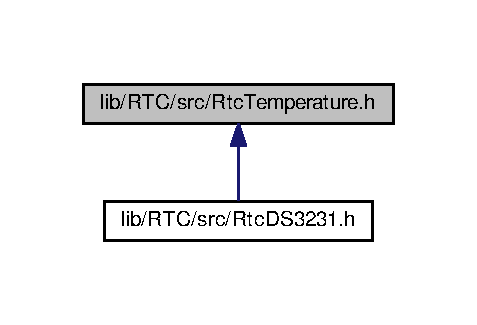
\includegraphics[width=229pt]{_rtc_temperature_8h__dep__incl}
\end{center}
\end{figure}
\subsection*{Classes}
\begin{DoxyCompactItemize}
\item 
class \hyperlink{class_rtc_temperature}{Rtc\+Temperature}
\end{DoxyCompactItemize}

\hypertarget{_rtc_utility_8cpp}{}\section{lib/\+R\+T\+C/src/\+Rtc\+Utility.cpp File Reference}
\label{_rtc_utility_8cpp}\index{lib/\+R\+T\+C/src/\+Rtc\+Utility.\+cpp@{lib/\+R\+T\+C/src/\+Rtc\+Utility.\+cpp}}
{\ttfamily \#include $<$Arduino.\+h$>$}\\*
{\ttfamily \#include $<$avr/pgmspace.\+h$>$}\\*
{\ttfamily \#include \char`\"{}Rtc\+Utility.\+h\char`\"{}}\\*
Include dependency graph for Rtc\+Utility.\+cpp\+:\nopagebreak
\begin{figure}[H]
\begin{center}
\leavevmode
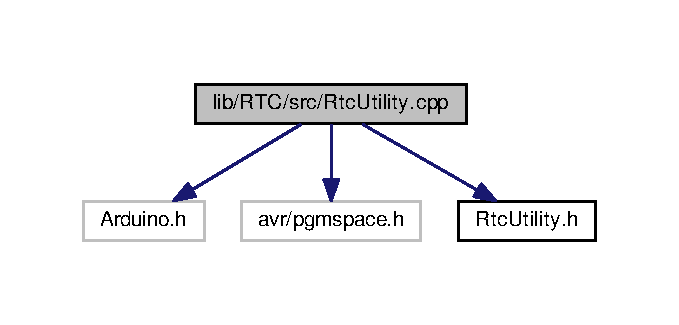
\includegraphics[width=326pt]{_rtc_utility_8cpp__incl}
\end{center}
\end{figure}
\subsection*{Functions}
\begin{DoxyCompactItemize}
\item 
uint8\+\_\+t \hyperlink{_rtc_utility_8cpp_a19597cd8048e5edad9e16a0ef50ccaad}{Bcd\+To\+Uint8} (uint8\+\_\+t val)
\item 
uint8\+\_\+t \hyperlink{_rtc_utility_8cpp_a82dafe67c162d761a8ebeaa5b40eeb50}{Uint8\+To\+Bcd} (uint8\+\_\+t val)
\item 
uint8\+\_\+t \hyperlink{_rtc_utility_8cpp_a6c80259aa408475f9dbd3c591a6d53cd}{Bcd\+To\+Bin24\+Hour} (uint8\+\_\+t bcd\+Hour)
\end{DoxyCompactItemize}


\subsection{Function Documentation}
\index{Rtc\+Utility.\+cpp@{Rtc\+Utility.\+cpp}!Bcd\+To\+Bin24\+Hour@{Bcd\+To\+Bin24\+Hour}}
\index{Bcd\+To\+Bin24\+Hour@{Bcd\+To\+Bin24\+Hour}!Rtc\+Utility.\+cpp@{Rtc\+Utility.\+cpp}}
\subsubsection[{\texorpdfstring{Bcd\+To\+Bin24\+Hour(uint8\+\_\+t bcd\+Hour)}{BcdToBin24Hour(uint8_t bcdHour)}}]{\setlength{\rightskip}{0pt plus 5cm}uint8\+\_\+t Bcd\+To\+Bin24\+Hour (
\begin{DoxyParamCaption}
\item[{uint8\+\_\+t}]{bcd\+Hour}
\end{DoxyParamCaption}
)}\hypertarget{_rtc_utility_8cpp_a6c80259aa408475f9dbd3c591a6d53cd}{}\label{_rtc_utility_8cpp_a6c80259aa408475f9dbd3c591a6d53cd}


Definition at line 21 of file Rtc\+Utility.\+cpp.

\index{Rtc\+Utility.\+cpp@{Rtc\+Utility.\+cpp}!Bcd\+To\+Uint8@{Bcd\+To\+Uint8}}
\index{Bcd\+To\+Uint8@{Bcd\+To\+Uint8}!Rtc\+Utility.\+cpp@{Rtc\+Utility.\+cpp}}
\subsubsection[{\texorpdfstring{Bcd\+To\+Uint8(uint8\+\_\+t val)}{BcdToUint8(uint8_t val)}}]{\setlength{\rightskip}{0pt plus 5cm}uint8\+\_\+t Bcd\+To\+Uint8 (
\begin{DoxyParamCaption}
\item[{uint8\+\_\+t}]{val}
\end{DoxyParamCaption}
)}\hypertarget{_rtc_utility_8cpp_a19597cd8048e5edad9e16a0ef50ccaad}{}\label{_rtc_utility_8cpp_a19597cd8048e5edad9e16a0ef50ccaad}


Definition at line 11 of file Rtc\+Utility.\+cpp.

\index{Rtc\+Utility.\+cpp@{Rtc\+Utility.\+cpp}!Uint8\+To\+Bcd@{Uint8\+To\+Bcd}}
\index{Uint8\+To\+Bcd@{Uint8\+To\+Bcd}!Rtc\+Utility.\+cpp@{Rtc\+Utility.\+cpp}}
\subsubsection[{\texorpdfstring{Uint8\+To\+Bcd(uint8\+\_\+t val)}{Uint8ToBcd(uint8_t val)}}]{\setlength{\rightskip}{0pt plus 5cm}uint8\+\_\+t Uint8\+To\+Bcd (
\begin{DoxyParamCaption}
\item[{uint8\+\_\+t}]{val}
\end{DoxyParamCaption}
)}\hypertarget{_rtc_utility_8cpp_a82dafe67c162d761a8ebeaa5b40eeb50}{}\label{_rtc_utility_8cpp_a82dafe67c162d761a8ebeaa5b40eeb50}


Definition at line 16 of file Rtc\+Utility.\+cpp.


\hypertarget{_rtc_utility_8h}{}\section{lib/\+R\+T\+C/src/\+Rtc\+Utility.h File Reference}
\label{_rtc_utility_8h}\index{lib/\+R\+T\+C/src/\+Rtc\+Utility.\+h@{lib/\+R\+T\+C/src/\+Rtc\+Utility.\+h}}
This graph shows which files directly or indirectly include this file\+:\nopagebreak
\begin{figure}[H]
\begin{center}
\leavevmode
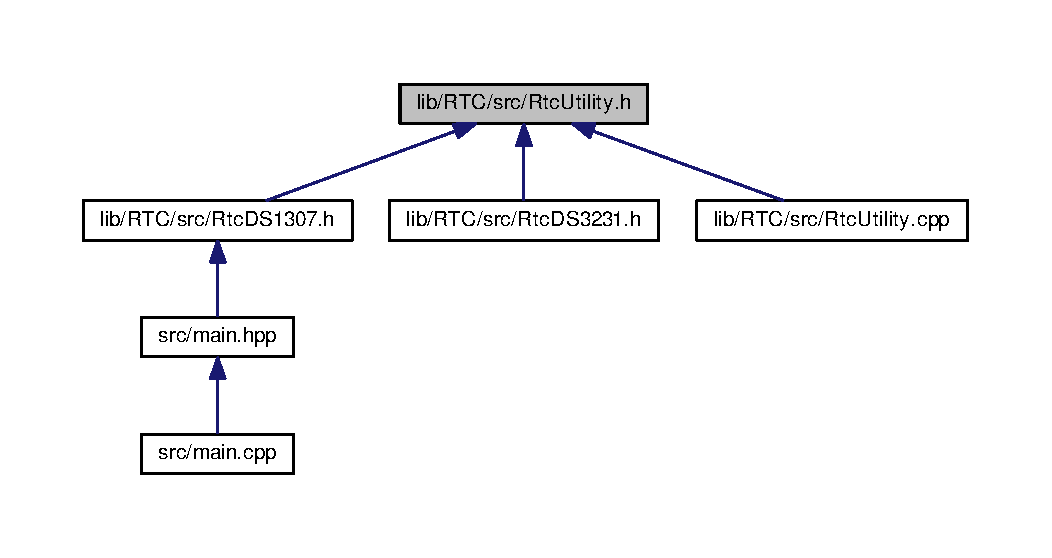
\includegraphics[width=350pt]{_rtc_utility_8h__dep__incl}
\end{center}
\end{figure}
\subsection*{Macros}
\begin{DoxyCompactItemize}
\item 
\#define \hyperlink{_rtc_utility_8h_a7d425596273d3668a700af992b2c1965}{\+\_\+\+BV}(b)~(1\+U\+L $<$$<$ (b))
\end{DoxyCompactItemize}
\subsection*{Functions}
\begin{DoxyCompactItemize}
\item 
uint8\+\_\+t \hyperlink{_rtc_utility_8h_a19597cd8048e5edad9e16a0ef50ccaad}{Bcd\+To\+Uint8} (uint8\+\_\+t val)
\item 
uint8\+\_\+t \hyperlink{_rtc_utility_8h_a82dafe67c162d761a8ebeaa5b40eeb50}{Uint8\+To\+Bcd} (uint8\+\_\+t val)
\item 
uint8\+\_\+t \hyperlink{_rtc_utility_8h_a6c80259aa408475f9dbd3c591a6d53cd}{Bcd\+To\+Bin24\+Hour} (uint8\+\_\+t bcd\+Hour)
\end{DoxyCompactItemize}


\subsection{Macro Definition Documentation}
\index{Rtc\+Utility.\+h@{Rtc\+Utility.\+h}!\+\_\+\+BV@{\+\_\+\+BV}}
\index{\+\_\+\+BV@{\+\_\+\+BV}!Rtc\+Utility.\+h@{Rtc\+Utility.\+h}}
\subsubsection[{\texorpdfstring{\+\_\+\+BV}{_BV}}]{\setlength{\rightskip}{0pt plus 5cm}\#define \+\_\+\+BV(
\begin{DoxyParamCaption}
\item[{}]{b}
\end{DoxyParamCaption}
)~(1\+U\+L $<$$<$ (b))}\hypertarget{_rtc_utility_8h_a7d425596273d3668a700af992b2c1965}{}\label{_rtc_utility_8h_a7d425596273d3668a700af992b2c1965}


Definition at line 7 of file Rtc\+Utility.\+h.



\subsection{Function Documentation}
\index{Rtc\+Utility.\+h@{Rtc\+Utility.\+h}!Bcd\+To\+Bin24\+Hour@{Bcd\+To\+Bin24\+Hour}}
\index{Bcd\+To\+Bin24\+Hour@{Bcd\+To\+Bin24\+Hour}!Rtc\+Utility.\+h@{Rtc\+Utility.\+h}}
\subsubsection[{\texorpdfstring{Bcd\+To\+Bin24\+Hour(uint8\+\_\+t bcd\+Hour)}{BcdToBin24Hour(uint8_t bcdHour)}}]{\setlength{\rightskip}{0pt plus 5cm}uint8\+\_\+t Bcd\+To\+Bin24\+Hour (
\begin{DoxyParamCaption}
\item[{uint8\+\_\+t}]{bcd\+Hour}
\end{DoxyParamCaption}
)}\hypertarget{_rtc_utility_8h_a6c80259aa408475f9dbd3c591a6d53cd}{}\label{_rtc_utility_8h_a6c80259aa408475f9dbd3c591a6d53cd}


Definition at line 21 of file Rtc\+Utility.\+cpp.

\index{Rtc\+Utility.\+h@{Rtc\+Utility.\+h}!Bcd\+To\+Uint8@{Bcd\+To\+Uint8}}
\index{Bcd\+To\+Uint8@{Bcd\+To\+Uint8}!Rtc\+Utility.\+h@{Rtc\+Utility.\+h}}
\subsubsection[{\texorpdfstring{Bcd\+To\+Uint8(uint8\+\_\+t val)}{BcdToUint8(uint8_t val)}}]{\setlength{\rightskip}{0pt plus 5cm}uint8\+\_\+t Bcd\+To\+Uint8 (
\begin{DoxyParamCaption}
\item[{uint8\+\_\+t}]{val}
\end{DoxyParamCaption}
)}\hypertarget{_rtc_utility_8h_a19597cd8048e5edad9e16a0ef50ccaad}{}\label{_rtc_utility_8h_a19597cd8048e5edad9e16a0ef50ccaad}


Definition at line 11 of file Rtc\+Utility.\+cpp.

\index{Rtc\+Utility.\+h@{Rtc\+Utility.\+h}!Uint8\+To\+Bcd@{Uint8\+To\+Bcd}}
\index{Uint8\+To\+Bcd@{Uint8\+To\+Bcd}!Rtc\+Utility.\+h@{Rtc\+Utility.\+h}}
\subsubsection[{\texorpdfstring{Uint8\+To\+Bcd(uint8\+\_\+t val)}{Uint8ToBcd(uint8_t val)}}]{\setlength{\rightskip}{0pt plus 5cm}uint8\+\_\+t Uint8\+To\+Bcd (
\begin{DoxyParamCaption}
\item[{uint8\+\_\+t}]{val}
\end{DoxyParamCaption}
)}\hypertarget{_rtc_utility_8h_a82dafe67c162d761a8ebeaa5b40eeb50}{}\label{_rtc_utility_8h_a82dafe67c162d761a8ebeaa5b40eeb50}


Definition at line 16 of file Rtc\+Utility.\+cpp.


\hypertarget{_tiny_g_p_s_09_09_8cpp}{}\section{lib/\+Tiny\+G\+P\+S\+Plus/\+Tiny\+G\+P\+S++.cpp File Reference}
\label{_tiny_g_p_s_09_09_8cpp}\index{lib/\+Tiny\+G\+P\+S\+Plus/\+Tiny\+G\+P\+S++.\+cpp@{lib/\+Tiny\+G\+P\+S\+Plus/\+Tiny\+G\+P\+S++.\+cpp}}
{\ttfamily \#include \char`\"{}Tiny\+G\+P\+S++.\+h\char`\"{}}\\*
{\ttfamily \#include $<$string.\+h$>$}\\*
{\ttfamily \#include $<$ctype.\+h$>$}\\*
{\ttfamily \#include $<$stdlib.\+h$>$}\\*
Include dependency graph for Tiny\+G\+P\+S++.cpp\+:\nopagebreak
\begin{figure}[H]
\begin{center}
\leavevmode
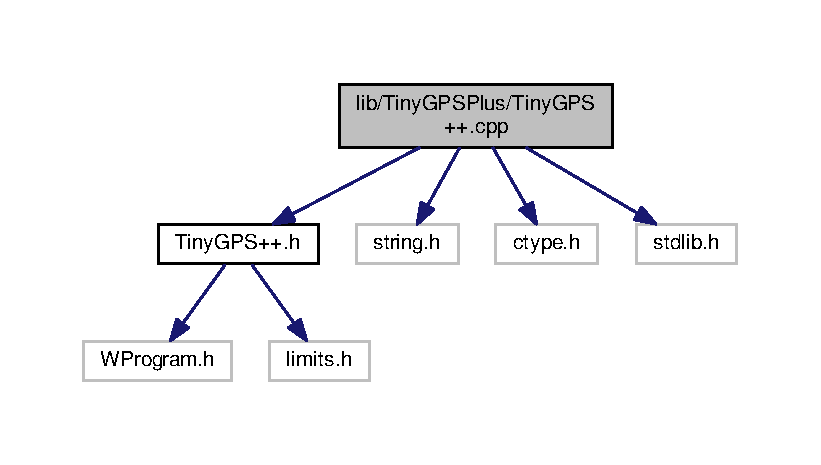
\includegraphics[width=350pt]{_tiny_g_p_s_09_09_8cpp__incl}
\end{center}
\end{figure}
\subsection*{Macros}
\begin{DoxyCompactItemize}
\item 
\#define \hyperlink{_tiny_g_p_s_09_09_8cpp_a6233d7d8f4845843775224f7521595bf}{\+\_\+\+G\+P\+R\+M\+Cterm}~\char`\"{}G\+P\+R\+MC\char`\"{}
\item 
\#define \hyperlink{_tiny_g_p_s_09_09_8cpp_a56d2fdf2ce63d8f36c1a6a82fcdcfe4e}{\+\_\+\+G\+N\+R\+M\+Cterm}~\char`\"{}G\+N\+R\+MC\char`\"{}
\item 
\#define \hyperlink{_tiny_g_p_s_09_09_8cpp_a7b0531ec5f337570bebda67aef146173}{\+\_\+\+G\+P\+G\+G\+Aterm}~\char`\"{}G\+P\+G\+GA\char`\"{}
\item 
\#define \hyperlink{_tiny_g_p_s_09_09_8cpp_ae28873e01fa28eec31295762b3f55337}{\+\_\+\+G\+N\+G\+G\+Aterm}~\char`\"{}G\+N\+G\+GA\char`\"{}
\item 
\#define \hyperlink{_tiny_g_p_s_09_09_8cpp_ae8b0c7d4f4c61109a44d953e5bd22e4f}{C\+O\+M\+B\+I\+NE}(sentence\+\_\+type,  term\+\_\+number)~(((unsigned)(sentence\+\_\+type) $<$$<$ 5) $\vert$ term\+\_\+number)
\end{DoxyCompactItemize}


\subsection{Macro Definition Documentation}
\index{Tiny\+G\+P\+S++.\+cpp@{Tiny\+G\+P\+S++.\+cpp}!\+\_\+\+G\+N\+G\+G\+Aterm@{\+\_\+\+G\+N\+G\+G\+Aterm}}
\index{\+\_\+\+G\+N\+G\+G\+Aterm@{\+\_\+\+G\+N\+G\+G\+Aterm}!Tiny\+G\+P\+S++.\+cpp@{Tiny\+G\+P\+S++.\+cpp}}
\subsubsection[{\texorpdfstring{\+\_\+\+G\+N\+G\+G\+Aterm}{_GNGGAterm}}]{\setlength{\rightskip}{0pt plus 5cm}\#define \+\_\+\+G\+N\+G\+G\+Aterm~\char`\"{}G\+N\+G\+GA\char`\"{}}\hypertarget{_tiny_g_p_s_09_09_8cpp_ae28873e01fa28eec31295762b3f55337}{}\label{_tiny_g_p_s_09_09_8cpp_ae28873e01fa28eec31295762b3f55337}


Definition at line 33 of file Tiny\+G\+P\+S++.\+cpp.

\index{Tiny\+G\+P\+S++.\+cpp@{Tiny\+G\+P\+S++.\+cpp}!\+\_\+\+G\+N\+R\+M\+Cterm@{\+\_\+\+G\+N\+R\+M\+Cterm}}
\index{\+\_\+\+G\+N\+R\+M\+Cterm@{\+\_\+\+G\+N\+R\+M\+Cterm}!Tiny\+G\+P\+S++.\+cpp@{Tiny\+G\+P\+S++.\+cpp}}
\subsubsection[{\texorpdfstring{\+\_\+\+G\+N\+R\+M\+Cterm}{_GNRMCterm}}]{\setlength{\rightskip}{0pt plus 5cm}\#define \+\_\+\+G\+N\+R\+M\+Cterm~\char`\"{}G\+N\+R\+MC\char`\"{}}\hypertarget{_tiny_g_p_s_09_09_8cpp_a56d2fdf2ce63d8f36c1a6a82fcdcfe4e}{}\label{_tiny_g_p_s_09_09_8cpp_a56d2fdf2ce63d8f36c1a6a82fcdcfe4e}


Definition at line 31 of file Tiny\+G\+P\+S++.\+cpp.

\index{Tiny\+G\+P\+S++.\+cpp@{Tiny\+G\+P\+S++.\+cpp}!\+\_\+\+G\+P\+G\+G\+Aterm@{\+\_\+\+G\+P\+G\+G\+Aterm}}
\index{\+\_\+\+G\+P\+G\+G\+Aterm@{\+\_\+\+G\+P\+G\+G\+Aterm}!Tiny\+G\+P\+S++.\+cpp@{Tiny\+G\+P\+S++.\+cpp}}
\subsubsection[{\texorpdfstring{\+\_\+\+G\+P\+G\+G\+Aterm}{_GPGGAterm}}]{\setlength{\rightskip}{0pt plus 5cm}\#define \+\_\+\+G\+P\+G\+G\+Aterm~\char`\"{}G\+P\+G\+GA\char`\"{}}\hypertarget{_tiny_g_p_s_09_09_8cpp_a7b0531ec5f337570bebda67aef146173}{}\label{_tiny_g_p_s_09_09_8cpp_a7b0531ec5f337570bebda67aef146173}


Definition at line 32 of file Tiny\+G\+P\+S++.\+cpp.

\index{Tiny\+G\+P\+S++.\+cpp@{Tiny\+G\+P\+S++.\+cpp}!\+\_\+\+G\+P\+R\+M\+Cterm@{\+\_\+\+G\+P\+R\+M\+Cterm}}
\index{\+\_\+\+G\+P\+R\+M\+Cterm@{\+\_\+\+G\+P\+R\+M\+Cterm}!Tiny\+G\+P\+S++.\+cpp@{Tiny\+G\+P\+S++.\+cpp}}
\subsubsection[{\texorpdfstring{\+\_\+\+G\+P\+R\+M\+Cterm}{_GPRMCterm}}]{\setlength{\rightskip}{0pt plus 5cm}\#define \+\_\+\+G\+P\+R\+M\+Cterm~\char`\"{}G\+P\+R\+MC\char`\"{}}\hypertarget{_tiny_g_p_s_09_09_8cpp_a6233d7d8f4845843775224f7521595bf}{}\label{_tiny_g_p_s_09_09_8cpp_a6233d7d8f4845843775224f7521595bf}


Definition at line 30 of file Tiny\+G\+P\+S++.\+cpp.

\index{Tiny\+G\+P\+S++.\+cpp@{Tiny\+G\+P\+S++.\+cpp}!C\+O\+M\+B\+I\+NE@{C\+O\+M\+B\+I\+NE}}
\index{C\+O\+M\+B\+I\+NE@{C\+O\+M\+B\+I\+NE}!Tiny\+G\+P\+S++.\+cpp@{Tiny\+G\+P\+S++.\+cpp}}
\subsubsection[{\texorpdfstring{C\+O\+M\+B\+I\+NE}{COMBINE}}]{\setlength{\rightskip}{0pt plus 5cm}\#define C\+O\+M\+B\+I\+NE(
\begin{DoxyParamCaption}
\item[{}]{sentence\+\_\+type, }
\item[{}]{term\+\_\+number}
\end{DoxyParamCaption}
)~(((unsigned)(sentence\+\_\+type) $<$$<$ 5) $\vert$ term\+\_\+number)}\hypertarget{_tiny_g_p_s_09_09_8cpp_ae8b0c7d4f4c61109a44d953e5bd22e4f}{}\label{_tiny_g_p_s_09_09_8cpp_ae8b0c7d4f4c61109a44d953e5bd22e4f}


Definition at line 155 of file Tiny\+G\+P\+S++.\+cpp.


\hypertarget{_tiny_g_p_s_09_09_8h}{}\section{lib/\+Tiny\+G\+P\+S\+Plus/\+Tiny\+G\+P\+S++.h File Reference}
\label{_tiny_g_p_s_09_09_8h}\index{lib/\+Tiny\+G\+P\+S\+Plus/\+Tiny\+G\+P\+S++.\+h@{lib/\+Tiny\+G\+P\+S\+Plus/\+Tiny\+G\+P\+S++.\+h}}
{\ttfamily \#include \char`\"{}W\+Program.\+h\char`\"{}}\\*
{\ttfamily \#include $<$limits.\+h$>$}\\*
Include dependency graph for Tiny\+G\+P\+S++.h\+:\nopagebreak
\begin{figure}[H]
\begin{center}
\leavevmode
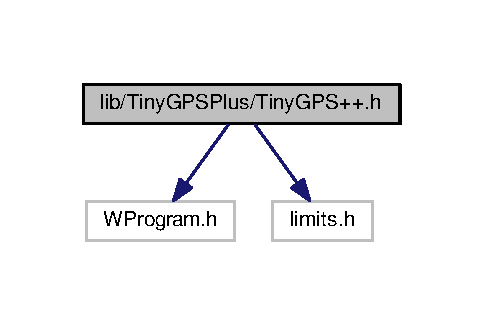
\includegraphics[width=232pt]{_tiny_g_p_s_09_09_8h__incl}
\end{center}
\end{figure}
This graph shows which files directly or indirectly include this file\+:\nopagebreak
\begin{figure}[H]
\begin{center}
\leavevmode
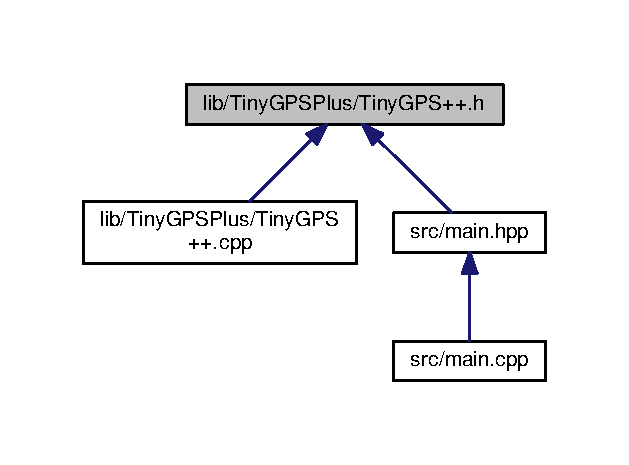
\includegraphics[width=302pt]{_tiny_g_p_s_09_09_8h__dep__incl}
\end{center}
\end{figure}
\subsection*{Classes}
\begin{DoxyCompactItemize}
\item 
struct \hyperlink{struct_raw_degrees}{Raw\+Degrees}
\item 
struct \hyperlink{struct_tiny_g_p_s_location}{Tiny\+G\+P\+S\+Location}
\item 
struct \hyperlink{struct_tiny_g_p_s_date}{Tiny\+G\+P\+S\+Date}
\item 
struct \hyperlink{struct_tiny_g_p_s_time}{Tiny\+G\+P\+S\+Time}
\item 
struct \hyperlink{struct_tiny_g_p_s_decimal}{Tiny\+G\+P\+S\+Decimal}
\item 
struct \hyperlink{struct_tiny_g_p_s_integer}{Tiny\+G\+P\+S\+Integer}
\item 
struct \hyperlink{struct_tiny_g_p_s_speed}{Tiny\+G\+P\+S\+Speed}
\item 
struct \hyperlink{struct_tiny_g_p_s_course}{Tiny\+G\+P\+S\+Course}
\item 
struct \hyperlink{struct_tiny_g_p_s_altitude}{Tiny\+G\+P\+S\+Altitude}
\item 
class \hyperlink{class_tiny_g_p_s_custom}{Tiny\+G\+P\+S\+Custom}
\item 
class \hyperlink{class_tiny_g_p_s_plus}{Tiny\+G\+P\+S\+Plus}
\end{DoxyCompactItemize}
\subsection*{Macros}
\begin{DoxyCompactItemize}
\item 
\#define \hyperlink{_tiny_g_p_s_09_09_8h_a210404d704c58b910ecee5bd7e97a7dc}{\+\_\+\+G\+P\+S\+\_\+\+V\+E\+R\+S\+I\+ON}~\char`\"{}0.\+95\char`\"{}
\item 
\#define \hyperlink{_tiny_g_p_s_09_09_8h_a15c78046c05b411cbcb3f93b7a452a97}{\+\_\+\+G\+P\+S\+\_\+\+M\+P\+H\+\_\+\+P\+E\+R\+\_\+\+K\+N\+OT}~1.\+15077945
\item 
\#define \hyperlink{_tiny_g_p_s_09_09_8h_a54cbb270522b52fe2c0f14eab76f032b}{\+\_\+\+G\+P\+S\+\_\+\+M\+P\+S\+\_\+\+P\+E\+R\+\_\+\+K\+N\+OT}~0.\+51444444
\item 
\#define \hyperlink{_tiny_g_p_s_09_09_8h_a757cab8e33085416dbafbc05cf71f6a9}{\+\_\+\+G\+P\+S\+\_\+\+K\+M\+P\+H\+\_\+\+P\+E\+R\+\_\+\+K\+N\+OT}~1.\+852
\item 
\#define \hyperlink{_tiny_g_p_s_09_09_8h_a51d2cc47a0dc5655cde4135c24fef480}{\+\_\+\+G\+P\+S\+\_\+\+M\+I\+L\+E\+S\+\_\+\+P\+E\+R\+\_\+\+M\+E\+T\+ER}~0.\+00062137112
\item 
\#define \hyperlink{_tiny_g_p_s_09_09_8h_a49b3ac6a23c4f78931942c51810e3439}{\+\_\+\+G\+P\+S\+\_\+\+K\+M\+\_\+\+P\+E\+R\+\_\+\+M\+E\+T\+ER}~0.\+001
\item 
\#define \hyperlink{_tiny_g_p_s_09_09_8h_af1a3b64121f34d416925518e994b454f}{\+\_\+\+G\+P\+S\+\_\+\+F\+E\+E\+T\+\_\+\+P\+E\+R\+\_\+\+M\+E\+T\+ER}~3.\+2808399
\item 
\#define \hyperlink{_tiny_g_p_s_09_09_8h_ad31ceaaeae16e1ff8e13640e3b012de3}{\+\_\+\+G\+P\+S\+\_\+\+M\+A\+X\+\_\+\+F\+I\+E\+L\+D\+\_\+\+S\+I\+ZE}~15
\end{DoxyCompactItemize}


\subsection{Macro Definition Documentation}
\index{Tiny\+G\+P\+S++.\+h@{Tiny\+G\+P\+S++.\+h}!\+\_\+\+G\+P\+S\+\_\+\+F\+E\+E\+T\+\_\+\+P\+E\+R\+\_\+\+M\+E\+T\+ER@{\+\_\+\+G\+P\+S\+\_\+\+F\+E\+E\+T\+\_\+\+P\+E\+R\+\_\+\+M\+E\+T\+ER}}
\index{\+\_\+\+G\+P\+S\+\_\+\+F\+E\+E\+T\+\_\+\+P\+E\+R\+\_\+\+M\+E\+T\+ER@{\+\_\+\+G\+P\+S\+\_\+\+F\+E\+E\+T\+\_\+\+P\+E\+R\+\_\+\+M\+E\+T\+ER}!Tiny\+G\+P\+S++.\+h@{Tiny\+G\+P\+S++.\+h}}
\subsubsection[{\texorpdfstring{\+\_\+\+G\+P\+S\+\_\+\+F\+E\+E\+T\+\_\+\+P\+E\+R\+\_\+\+M\+E\+T\+ER}{_GPS_FEET_PER_METER}}]{\setlength{\rightskip}{0pt plus 5cm}\#define \+\_\+\+G\+P\+S\+\_\+\+F\+E\+E\+T\+\_\+\+P\+E\+R\+\_\+\+M\+E\+T\+ER~3.\+2808399}\hypertarget{_tiny_g_p_s_09_09_8h_af1a3b64121f34d416925518e994b454f}{}\label{_tiny_g_p_s_09_09_8h_af1a3b64121f34d416925518e994b454f}


Definition at line 40 of file Tiny\+G\+P\+S++.\+h.

\index{Tiny\+G\+P\+S++.\+h@{Tiny\+G\+P\+S++.\+h}!\+\_\+\+G\+P\+S\+\_\+\+K\+M\+\_\+\+P\+E\+R\+\_\+\+M\+E\+T\+ER@{\+\_\+\+G\+P\+S\+\_\+\+K\+M\+\_\+\+P\+E\+R\+\_\+\+M\+E\+T\+ER}}
\index{\+\_\+\+G\+P\+S\+\_\+\+K\+M\+\_\+\+P\+E\+R\+\_\+\+M\+E\+T\+ER@{\+\_\+\+G\+P\+S\+\_\+\+K\+M\+\_\+\+P\+E\+R\+\_\+\+M\+E\+T\+ER}!Tiny\+G\+P\+S++.\+h@{Tiny\+G\+P\+S++.\+h}}
\subsubsection[{\texorpdfstring{\+\_\+\+G\+P\+S\+\_\+\+K\+M\+\_\+\+P\+E\+R\+\_\+\+M\+E\+T\+ER}{_GPS_KM_PER_METER}}]{\setlength{\rightskip}{0pt plus 5cm}\#define \+\_\+\+G\+P\+S\+\_\+\+K\+M\+\_\+\+P\+E\+R\+\_\+\+M\+E\+T\+ER~0.\+001}\hypertarget{_tiny_g_p_s_09_09_8h_a49b3ac6a23c4f78931942c51810e3439}{}\label{_tiny_g_p_s_09_09_8h_a49b3ac6a23c4f78931942c51810e3439}


Definition at line 39 of file Tiny\+G\+P\+S++.\+h.

\index{Tiny\+G\+P\+S++.\+h@{Tiny\+G\+P\+S++.\+h}!\+\_\+\+G\+P\+S\+\_\+\+K\+M\+P\+H\+\_\+\+P\+E\+R\+\_\+\+K\+N\+OT@{\+\_\+\+G\+P\+S\+\_\+\+K\+M\+P\+H\+\_\+\+P\+E\+R\+\_\+\+K\+N\+OT}}
\index{\+\_\+\+G\+P\+S\+\_\+\+K\+M\+P\+H\+\_\+\+P\+E\+R\+\_\+\+K\+N\+OT@{\+\_\+\+G\+P\+S\+\_\+\+K\+M\+P\+H\+\_\+\+P\+E\+R\+\_\+\+K\+N\+OT}!Tiny\+G\+P\+S++.\+h@{Tiny\+G\+P\+S++.\+h}}
\subsubsection[{\texorpdfstring{\+\_\+\+G\+P\+S\+\_\+\+K\+M\+P\+H\+\_\+\+P\+E\+R\+\_\+\+K\+N\+OT}{_GPS_KMPH_PER_KNOT}}]{\setlength{\rightskip}{0pt plus 5cm}\#define \+\_\+\+G\+P\+S\+\_\+\+K\+M\+P\+H\+\_\+\+P\+E\+R\+\_\+\+K\+N\+OT~1.\+852}\hypertarget{_tiny_g_p_s_09_09_8h_a757cab8e33085416dbafbc05cf71f6a9}{}\label{_tiny_g_p_s_09_09_8h_a757cab8e33085416dbafbc05cf71f6a9}


Definition at line 37 of file Tiny\+G\+P\+S++.\+h.

\index{Tiny\+G\+P\+S++.\+h@{Tiny\+G\+P\+S++.\+h}!\+\_\+\+G\+P\+S\+\_\+\+M\+A\+X\+\_\+\+F\+I\+E\+L\+D\+\_\+\+S\+I\+ZE@{\+\_\+\+G\+P\+S\+\_\+\+M\+A\+X\+\_\+\+F\+I\+E\+L\+D\+\_\+\+S\+I\+ZE}}
\index{\+\_\+\+G\+P\+S\+\_\+\+M\+A\+X\+\_\+\+F\+I\+E\+L\+D\+\_\+\+S\+I\+ZE@{\+\_\+\+G\+P\+S\+\_\+\+M\+A\+X\+\_\+\+F\+I\+E\+L\+D\+\_\+\+S\+I\+ZE}!Tiny\+G\+P\+S++.\+h@{Tiny\+G\+P\+S++.\+h}}
\subsubsection[{\texorpdfstring{\+\_\+\+G\+P\+S\+\_\+\+M\+A\+X\+\_\+\+F\+I\+E\+L\+D\+\_\+\+S\+I\+ZE}{_GPS_MAX_FIELD_SIZE}}]{\setlength{\rightskip}{0pt plus 5cm}\#define \+\_\+\+G\+P\+S\+\_\+\+M\+A\+X\+\_\+\+F\+I\+E\+L\+D\+\_\+\+S\+I\+ZE~15}\hypertarget{_tiny_g_p_s_09_09_8h_ad31ceaaeae16e1ff8e13640e3b012de3}{}\label{_tiny_g_p_s_09_09_8h_ad31ceaaeae16e1ff8e13640e3b012de3}


Definition at line 41 of file Tiny\+G\+P\+S++.\+h.

\index{Tiny\+G\+P\+S++.\+h@{Tiny\+G\+P\+S++.\+h}!\+\_\+\+G\+P\+S\+\_\+\+M\+I\+L\+E\+S\+\_\+\+P\+E\+R\+\_\+\+M\+E\+T\+ER@{\+\_\+\+G\+P\+S\+\_\+\+M\+I\+L\+E\+S\+\_\+\+P\+E\+R\+\_\+\+M\+E\+T\+ER}}
\index{\+\_\+\+G\+P\+S\+\_\+\+M\+I\+L\+E\+S\+\_\+\+P\+E\+R\+\_\+\+M\+E\+T\+ER@{\+\_\+\+G\+P\+S\+\_\+\+M\+I\+L\+E\+S\+\_\+\+P\+E\+R\+\_\+\+M\+E\+T\+ER}!Tiny\+G\+P\+S++.\+h@{Tiny\+G\+P\+S++.\+h}}
\subsubsection[{\texorpdfstring{\+\_\+\+G\+P\+S\+\_\+\+M\+I\+L\+E\+S\+\_\+\+P\+E\+R\+\_\+\+M\+E\+T\+ER}{_GPS_MILES_PER_METER}}]{\setlength{\rightskip}{0pt plus 5cm}\#define \+\_\+\+G\+P\+S\+\_\+\+M\+I\+L\+E\+S\+\_\+\+P\+E\+R\+\_\+\+M\+E\+T\+ER~0.\+00062137112}\hypertarget{_tiny_g_p_s_09_09_8h_a51d2cc47a0dc5655cde4135c24fef480}{}\label{_tiny_g_p_s_09_09_8h_a51d2cc47a0dc5655cde4135c24fef480}


Definition at line 38 of file Tiny\+G\+P\+S++.\+h.

\index{Tiny\+G\+P\+S++.\+h@{Tiny\+G\+P\+S++.\+h}!\+\_\+\+G\+P\+S\+\_\+\+M\+P\+H\+\_\+\+P\+E\+R\+\_\+\+K\+N\+OT@{\+\_\+\+G\+P\+S\+\_\+\+M\+P\+H\+\_\+\+P\+E\+R\+\_\+\+K\+N\+OT}}
\index{\+\_\+\+G\+P\+S\+\_\+\+M\+P\+H\+\_\+\+P\+E\+R\+\_\+\+K\+N\+OT@{\+\_\+\+G\+P\+S\+\_\+\+M\+P\+H\+\_\+\+P\+E\+R\+\_\+\+K\+N\+OT}!Tiny\+G\+P\+S++.\+h@{Tiny\+G\+P\+S++.\+h}}
\subsubsection[{\texorpdfstring{\+\_\+\+G\+P\+S\+\_\+\+M\+P\+H\+\_\+\+P\+E\+R\+\_\+\+K\+N\+OT}{_GPS_MPH_PER_KNOT}}]{\setlength{\rightskip}{0pt plus 5cm}\#define \+\_\+\+G\+P\+S\+\_\+\+M\+P\+H\+\_\+\+P\+E\+R\+\_\+\+K\+N\+OT~1.\+15077945}\hypertarget{_tiny_g_p_s_09_09_8h_a15c78046c05b411cbcb3f93b7a452a97}{}\label{_tiny_g_p_s_09_09_8h_a15c78046c05b411cbcb3f93b7a452a97}


Definition at line 35 of file Tiny\+G\+P\+S++.\+h.

\index{Tiny\+G\+P\+S++.\+h@{Tiny\+G\+P\+S++.\+h}!\+\_\+\+G\+P\+S\+\_\+\+M\+P\+S\+\_\+\+P\+E\+R\+\_\+\+K\+N\+OT@{\+\_\+\+G\+P\+S\+\_\+\+M\+P\+S\+\_\+\+P\+E\+R\+\_\+\+K\+N\+OT}}
\index{\+\_\+\+G\+P\+S\+\_\+\+M\+P\+S\+\_\+\+P\+E\+R\+\_\+\+K\+N\+OT@{\+\_\+\+G\+P\+S\+\_\+\+M\+P\+S\+\_\+\+P\+E\+R\+\_\+\+K\+N\+OT}!Tiny\+G\+P\+S++.\+h@{Tiny\+G\+P\+S++.\+h}}
\subsubsection[{\texorpdfstring{\+\_\+\+G\+P\+S\+\_\+\+M\+P\+S\+\_\+\+P\+E\+R\+\_\+\+K\+N\+OT}{_GPS_MPS_PER_KNOT}}]{\setlength{\rightskip}{0pt plus 5cm}\#define \+\_\+\+G\+P\+S\+\_\+\+M\+P\+S\+\_\+\+P\+E\+R\+\_\+\+K\+N\+OT~0.\+51444444}\hypertarget{_tiny_g_p_s_09_09_8h_a54cbb270522b52fe2c0f14eab76f032b}{}\label{_tiny_g_p_s_09_09_8h_a54cbb270522b52fe2c0f14eab76f032b}


Definition at line 36 of file Tiny\+G\+P\+S++.\+h.

\index{Tiny\+G\+P\+S++.\+h@{Tiny\+G\+P\+S++.\+h}!\+\_\+\+G\+P\+S\+\_\+\+V\+E\+R\+S\+I\+ON@{\+\_\+\+G\+P\+S\+\_\+\+V\+E\+R\+S\+I\+ON}}
\index{\+\_\+\+G\+P\+S\+\_\+\+V\+E\+R\+S\+I\+ON@{\+\_\+\+G\+P\+S\+\_\+\+V\+E\+R\+S\+I\+ON}!Tiny\+G\+P\+S++.\+h@{Tiny\+G\+P\+S++.\+h}}
\subsubsection[{\texorpdfstring{\+\_\+\+G\+P\+S\+\_\+\+V\+E\+R\+S\+I\+ON}{_GPS_VERSION}}]{\setlength{\rightskip}{0pt plus 5cm}\#define \+\_\+\+G\+P\+S\+\_\+\+V\+E\+R\+S\+I\+ON~\char`\"{}0.\+95\char`\"{}}\hypertarget{_tiny_g_p_s_09_09_8h_a210404d704c58b910ecee5bd7e97a7dc}{}\label{_tiny_g_p_s_09_09_8h_a210404d704c58b910ecee5bd7e97a7dc}


Definition at line 34 of file Tiny\+G\+P\+S++.\+h.


\hypertarget{_r_e_a_d_m_e___p_t_b_r_8md}{}\section{R\+E\+A\+D\+M\+E\+\_\+\+P\+T\+B\+R.\+md File Reference}
\label{_r_e_a_d_m_e___p_t_b_r_8md}\index{R\+E\+A\+D\+M\+E\+\_\+\+P\+T\+B\+R.\+md@{R\+E\+A\+D\+M\+E\+\_\+\+P\+T\+B\+R.\+md}}

\hypertarget{main_8cpp}{}\section{src/main.cpp File Reference}
\label{main_8cpp}\index{src/main.\+cpp@{src/main.\+cpp}}
{\ttfamily \#include \char`\"{}Arduino.\+h\char`\"{}}\\*
{\ttfamily \#include \char`\"{}main.\+hpp\char`\"{}}\\*
Include dependency graph for main.\+cpp\+:\nopagebreak
\begin{figure}[H]
\begin{center}
\leavevmode
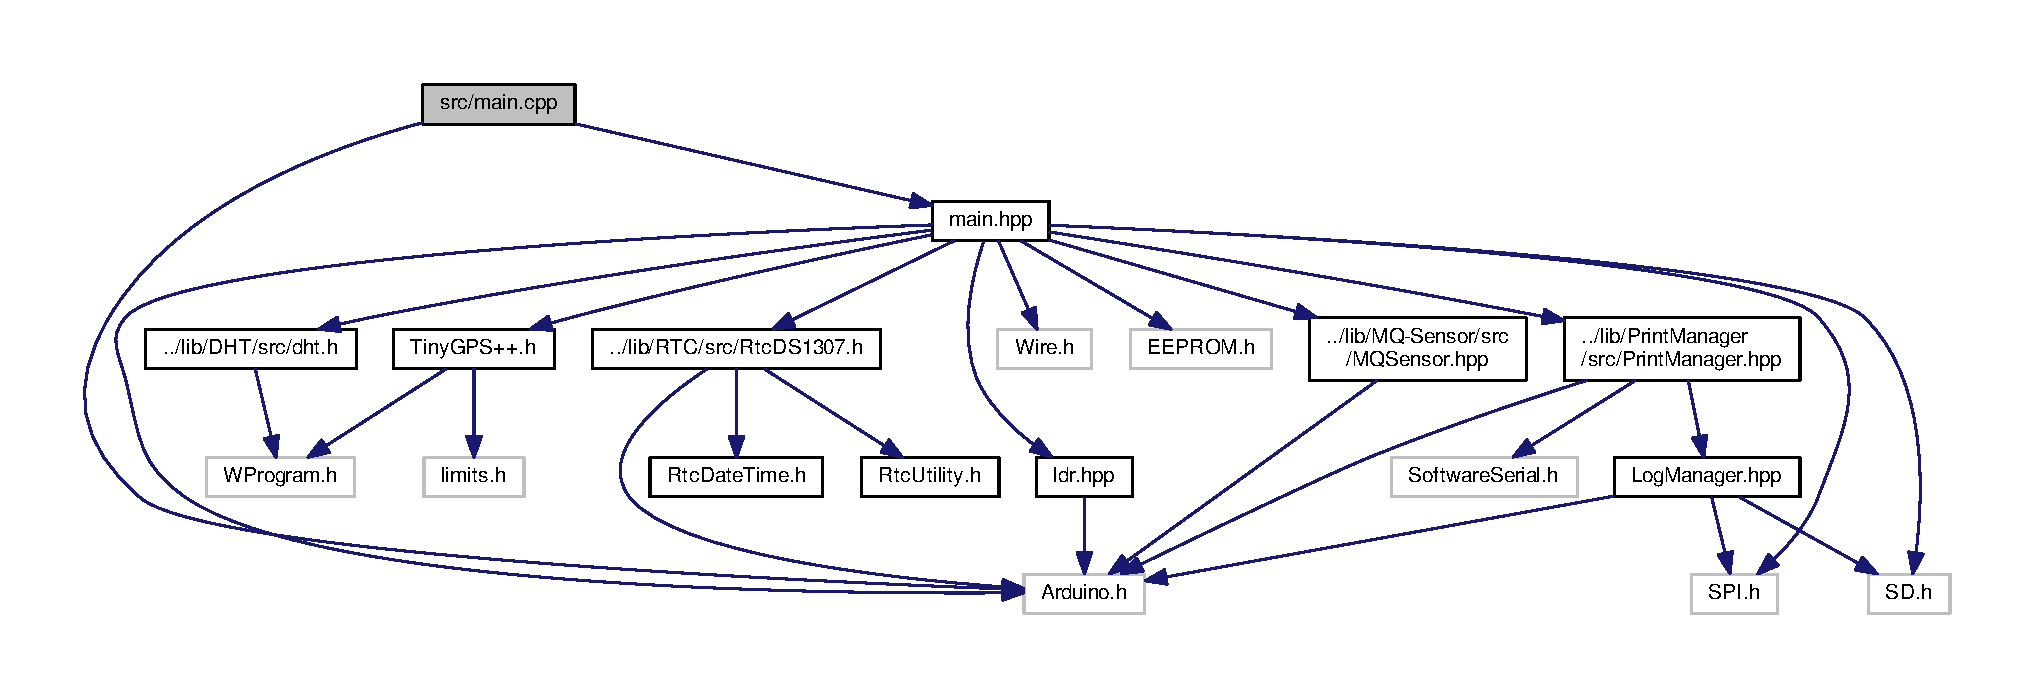
\includegraphics[width=350pt]{main_8cpp__incl}
\end{center}
\end{figure}
\subsection*{Functions}
\begin{DoxyCompactItemize}
\item 
void \hyperlink{main_8cpp_a4fc01d736fe50cf5b977f755b675f11d}{setup} ()
\item 
void \hyperlink{main_8cpp_afe461d27b9c48d5921c00d521181f12f}{loop} ()
\end{DoxyCompactItemize}


\subsection{Function Documentation}
\index{main.\+cpp@{main.\+cpp}!loop@{loop}}
\index{loop@{loop}!main.\+cpp@{main.\+cpp}}
\subsubsection[{\texorpdfstring{loop()}{loop()}}]{\setlength{\rightskip}{0pt plus 5cm}void loop (
\begin{DoxyParamCaption}
{}
\end{DoxyParamCaption}
)}\hypertarget{main_8cpp_afe461d27b9c48d5921c00d521181f12f}{}\label{main_8cpp_afe461d27b9c48d5921c00d521181f12f}


Definition at line 70 of file main.\+cpp.

\index{main.\+cpp@{main.\+cpp}!setup@{setup}}
\index{setup@{setup}!main.\+cpp@{main.\+cpp}}
\subsubsection[{\texorpdfstring{setup()}{setup()}}]{\setlength{\rightskip}{0pt plus 5cm}void setup (
\begin{DoxyParamCaption}
{}
\end{DoxyParamCaption}
)}\hypertarget{main_8cpp_a4fc01d736fe50cf5b977f755b675f11d}{}\label{main_8cpp_a4fc01d736fe50cf5b977f755b675f11d}


Definition at line 18 of file main.\+cpp.


\hypertarget{main_8hpp}{}\section{src/main.hpp File Reference}
\label{main_8hpp}\index{src/main.\+hpp@{src/main.\+hpp}}
{\ttfamily \#include \char`\"{}Arduino.\+h\char`\"{}}\\*
{\ttfamily \#include \char`\"{}dht.\+h\char`\"{}}\\*
Include dependency graph for main.\+hpp\+:
% FIG 0
This graph shows which files directly or indirectly include this file\+:
% FIG 1
\subsection*{Functions}
\begin{DoxyCompactItemize}
\item 
void \hyperlink{main_8hpp_a4a303c3b1de7cf54a8a5b31232355f74}{dht\+Debug} (\hyperlink{classdht}{dht} Sensor, uint8\+\_\+t \hyperlink{main_8cpp_a79111e78831efb8ac76fa8123357475e}{D\+H\+T11\+\_\+\+P\+IN})
\end{DoxyCompactItemize}


\subsection{Function Documentation}
\index{main.\+hpp@{main.\+hpp}!dht\+Debug@{dht\+Debug}}
\index{dht\+Debug@{dht\+Debug}!main.\+hpp@{main.\+hpp}}
\subsubsection[{\texorpdfstring{dht\+Debug(dht Sensor, uint8\+\_\+t D\+H\+T11\+\_\+\+P\+I\+N)}{dhtDebug(dht Sensor, uint8_t DHT11_PIN)}}]{\setlength{\rightskip}{0pt plus 5cm}void dht\+Debug (
\begin{DoxyParamCaption}
\item[{{\bf dht}}]{Sensor, }
\item[{uint8\+\_\+t}]{D\+H\+T11\+\_\+\+P\+IN}
\end{DoxyParamCaption}
)}\hypertarget{main_8hpp_a4a303c3b1de7cf54a8a5b31232355f74}{}\label{main_8hpp_a4a303c3b1de7cf54a8a5b31232355f74}


Definition at line 8 of file main.\+hpp.



Here is the call graph for this function\+:
% FIG 2




Here is the caller graph for this function\+:
% FIG 3



%--- End generated contents ---

% Index
\backmatter
\newpage
\phantomsection
\clearemptydoublepage
\addcontentsline{toc}{chapter}{Index}
\printindex

\end{document}
